% SWEVO_manuscript_full.tex -- single-file version of SWEVO_manuscript.tex, generated by analysis/flatten_swevo.py.
% All \input files and the generated tables and figures placed in the text are inlined. Needs: figures_mpce/,
% figures_final/ and (for references to the supplementary material, prefix S-) SWEVO_supplement.aux.
% Manuscript for Swarm and Evolutionary Computation (Elsevier), elsarticle preprint layout with line numbers.
% Same section files (optA/02_intro ... optA/10_limits_concl) and number macros as MPCE_PSO_VNS.tex; only the
% preamble, the front matter (optA/swevo_front.tex) and the back matter (optA/swevo_back.tex) are journal-specific.
% Build: sh analysis/build_swevo.sh (compiles SWEVO_supplement.tex and this file alternately; see optA/SWEVO.md).
\documentclass[preprint,12pt,number]{elsarticle}
% numbered references [1], [2], ... (natbib numbers; manual thebibliography in optA/swevo_back.tex);
% sort&compress gives [1-3] ranges as the cite package does in the MPCE version
\biboptions{sort&compress}
% A4 text block slightly larger than the elsarticle preprint default, so that the tallest generated table
% (analysis/mpce_tab_ablation.tex) fits on a page; \emergencystretch avoids overfull lines in the contribution list
\usepackage[a4paper,margin=2.5cm]{geometry}
\setlength{\emergencystretch}{1.5em}
% elsarticle 3.3 puts a stray space after the title-page footer box ("Preprint submitted to ..."), which gives an
% Overfull \hbox of about 2.6pt on page 1 in any document; absorb it (layout unchanged)
\makeatletter
\let\swevo@pprintTitle\ps@pprintTitle
\def\ps@pprintTitle{\swevo@pprintTitle\let\swevo@oddfoot\@oddfoot
  \def\@oddfoot{\hbox to\textwidth{\swevo@oddfoot\hss}}\let\@evenfoot\@oddfoot}
\makeatother
% continuous line numbers for review, starting after the title page (switched on right after \end{frontmatter};
% numbering the elsarticle title page itself pushes its footnotes into the footer)
\usepackage{lineno}
\usepackage{etoolbox}
\AfterEndEnvironment{frontmatter}{\linenumbers}
\usepackage{amsmath,amssymb,amsfonts}
\usepackage{algorithm}
\usepackage{algpseudocode}
\usepackage{booktabs}
\usepackage{graphicx}
\usepackage{textcomp}
\usepackage{multirow}
\usepackage{array}
\usepackage{xcolor}
\usepackage{url}
% References to the supplementary material (Tables S*, Figs. S*) are resolved from SWEVO_supplement.aux;
% build order: see analysis/build_swevo.sh (no hyperref: it would need xr-hyper and is not required by the journal)
\usepackage{xr}
\externaldocument[S-]{SWEVO_supplement}

\journal{Swarm and Evolutionary Computation}

% Visible placeholder for author information and for numbers whose runs are still pending
% (an empty argument, used in table cells, prints just [TBD])
\newcommand{\TBD}[1]{\textcolor{red}{[TBD\ifx\relax#1\relax\else: #1\fi]}}
% Every number quoted in the text: \N... macros generated by analysis/mpce_numbers.py from mpce_summary.json
% (a macro whose data are still missing expands to \TBD{pending: <experiments>}); same order as in MPCE_PSO_VNS.tex.
% Statements that depend on the outcome carry a comment "% CHECK-FINAL [Cnn]: <condition>";
% analysis/mpce_check_final.py evaluates these conditions (PASS / FAIL) after every run of mpce_results.py.
% >>>>> begin analysis/mpce_numbers.tex
% generated by mpce_numbers.py from mpce_summary.json (2026-09-29 01:27:40) -- do not edit by hand
% pending macros (expand to \TBD{pending: ...}): none
% data note: Horns Rev 16: all runs from mpce_hrfix (corrected direction binning, 970 runs); 1000 runs of the old model dropped
\newcommand{\NRunsMain}{16{,}320}
\newcommand{\NRunsBenchmark}{22{,}440}
\newcommand{\NFriedChi}{319.3}
\newcommand{\NFriedDf}{7}
\newcommand{\NFriedP}{\ensuremath{4.6\times10^{-65}}}
\newcommand{\NImanF}{136.5}
\newcommand{\NFriedVerb}{rejects}
\newcommand{\NRankPSOVNS}{1.82}
\newcommand{\NSoleBestPSOVNS}{29}
\newcommand{\NLossPSOVNS}{1.322}
\newcommand{\NFeasPSOVNS}{100.0}
\newcommand{\NRankPSO}{1.97}
\newcommand{\NSoleBestPSO}{25}
\newcommand{\NLossPSO}{1.341}
\newcommand{\NFeasPSO}{100.0}
\newcommand{\NRankSSAVNS}{3.45}
\newcommand{\NSoleBestSSAVNS}{0}
\newcommand{\NLossSSAVNS}{1.653}
\newcommand{\NFeasSSAVNS}{99.6}
\newcommand{\NRankSSA}{5.38}
\newcommand{\NSoleBestSSA}{0}
\newcommand{\NLossSSA}{1.805}
\newcommand{\NFeasSSA}{97.6}
\newcommand{\NRankLXSSA}{6.06}
\newcommand{\NSoleBestLXSSA}{0}
\newcommand{\NLossLXSSA}{1.959}
\newcommand{\NFeasLXSSA}{96.9}
\newcommand{\NRankDE}{7.04}
\newcommand{\NSoleBestDE}{0}
\newcommand{\NLossDE}{1.493}
\newcommand{\NFeasDE}{71.4}
\newcommand{\NRankVNS}{4.40}
\newcommand{\NSoleBestVNS}{3}
\newcommand{\NLossVNS}{1.788}
\newcommand{\NFeasVNS}{100.0}
\newcommand{\NRankSLSQP}{5.88}
\newcommand{\NSoleBestSLSQP}{1}
\newcommand{\NLossSLSQP}{1.758}
\newcommand{\NFeasSLSQP}{100.0}
\newcommand{\NRankFirst}{PSO-VNS}
\newcommand{\NRankOrderOthers}{PSO (1.97), SSA-VNS (3.45), VNS (4.40), SSA (5.38), MS-SLSQP (5.88), LX-SSA (6.06) and DE (7.04)}
\newcommand{\NPostHocSigList}{SSA-VNS, VNS, SSA, MS-SLSQP, LX-SSA and DE}
\newcommand{\NPostHocSigMaxP}{\ensuremath{2.1\times10^{-4}}}
\newcommand{\NPostHocNonSigList}{PSO}
\newcommand{\NPostHocNonSigP}{0.71}
\newcommand{\NWtlPSO}{14/50/4}
\newcommand{\NWtlPSOW}{14}
\newcommand{\NWtlPSOL}{4}
\newcommand{\NWtlPSOT}{50}
\newcommand{\NRrbPSO}{+0.08}
\newcommand{\NPWPSO}{0.30}
\newcommand{\NPWrawPSO}{0.30}
\newcommand{\NDLPSO}{\ensuremath{-}0.018}
\newcommand{\NDLabsPSO}{0.02}
\newcommand{\NLowerLossPSO}{34}
\newcommand{\NHigherLossPSO}{26}
\newcommand{\NWtlSSAVNS}{49/19/0}
\newcommand{\NWtlSSAVNSW}{49}
\newcommand{\NWtlSSAVNSL}{0}
\newcommand{\NWtlSSAVNST}{19}
\newcommand{\NRrbSSAVNS}{+0.72}
\newcommand{\NPWSSAVNS}{\ensuremath{5.7\times10^{-11}}}
\newcommand{\NPWrawSSAVNS}{\ensuremath{1.9\times10^{-11}}}
\newcommand{\NDLSSAVNS}{\ensuremath{-}0.330}
\newcommand{\NDLabsSSAVNS}{0.33}
\newcommand{\NLowerLossSSAVNS}{59}
\newcommand{\NHigherLossSSAVNS}{1}
\newcommand{\NWtlSSA}{59/9/0}
\newcommand{\NWtlSSAW}{59}
\newcommand{\NWtlSSAL}{0}
\newcommand{\NWtlSSAT}{9}
\newcommand{\NRrbSSA}{+0.98}
\newcommand{\NPWSSA}{\ensuremath{4.5\times10^{-11}}}
\newcommand{\NPWrawSSA}{\ensuremath{7.6\times10^{-12}}}
\newcommand{\NDLSSA}{\ensuremath{-}0.611}
\newcommand{\NDLabsSSA}{0.61}
\newcommand{\NLowerLossSSA}{60}
\newcommand{\NHigherLossSSA}{0}
\newcommand{\NWtlLXSSA}{60/8/0}
\newcommand{\NWtlLXSSAW}{60}
\newcommand{\NWtlLXSSAL}{0}
\newcommand{\NWtlLXSSAT}{8}
\newcommand{\NRrbLXSSA}{+0.97}
\newcommand{\NPWLXSSA}{\ensuremath{4.5\times10^{-11}}}
\newcommand{\NPWrawLXSSA}{\ensuremath{7.6\times10^{-12}}}
\newcommand{\NDLLXSSA}{\ensuremath{-}0.765}
\newcommand{\NDLabsLXSSA}{0.76}
\newcommand{\NLowerLossLXSSA}{60}
\newcommand{\NHigherLossLXSSA}{0}
\newcommand{\NWtlDE}{56/12/0}
\newcommand{\NWtlDEW}{56}
\newcommand{\NWtlDEL}{0}
\newcommand{\NWtlDET}{12}
\newcommand{\NRrbDE}{+1.00}
\newcommand{\NPWDE}{\ensuremath{5.6\times10^{-11}}}
\newcommand{\NPWrawDE}{\ensuremath{1.4\times10^{-11}}}
\newcommand{\NDLDE}{\ensuremath{-}0.887}
\newcommand{\NDLabsDE}{0.89}
\newcommand{\NLowerLossDE}{42}
\newcommand{\NHigherLossDE}{0}
\newcommand{\NWtlVNS}{51/16/1}
\newcommand{\NWtlVNSW}{51}
\newcommand{\NWtlVNSL}{1}
\newcommand{\NWtlVNST}{16}
\newcommand{\NRrbVNS}{+0.84}
\newcommand{\NPWVNS}{\ensuremath{1.3\times10^{-10}}}
\newcommand{\NPWrawVNS}{\ensuremath{6.3\times10^{-11}}}
\newcommand{\NDLVNS}{\ensuremath{-}0.465}
\newcommand{\NDLabsVNS}{0.47}
\newcommand{\NLowerLossVNS}{55}
\newcommand{\NHigherLossVNS}{4}
\newcommand{\NWtlSLSQP}{59/9/0}
\newcommand{\NWtlSLSQPW}{59}
\newcommand{\NWtlSLSQPL}{0}
\newcommand{\NWtlSLSQPT}{9}
\newcommand{\NRrbSLSQP}{+0.99}
\newcommand{\NPWSLSQP}{\ensuremath{4.2\times10^{-11}}}
\newcommand{\NPWrawSLSQP}{\ensuremath{6.0\times10^{-12}}}
\newcommand{\NDLSLSQP}{\ensuremath{-}0.435}
\newcommand{\NDLabsSLSQP}{0.44}
\newcommand{\NLowerLossSLSQP}{66}
\newcommand{\NHigherLossSLSQP}{2}
\newcommand{\NWtlPSOSig}{18}
\newcommand{\NNLarge}{20}
\newcommand{\NWtlPSOLargeW}{9}
\newcommand{\NWtlPSOLargeL}{2}
\newcommand{\NWtlPSOSmallW}{5}
\newcommand{\NWtlPSOSmallL}{2}
\newcommand{\NGainPSOLarge}{0.08}
\newcommand{\NAbsDiffPSOSmall}{0.03}
\newcommand{\NLossesPhrase}{it is never significantly worse than SSA-VNS, SSA, LX-SSA, DE and MS-SLSQP and significantly worse than VNS in one case}
\newcommand{\NLossMaxSmallN}{0.25}
\newcommand{\NLossBigIPSOVNS}{1.60}
\newcommand{\NLossBigIPSO}{1.62}
\newcommand{\NLossBigISSAVNS}{1.69}
\newcommand{\NLossBigISSA}{2.80}
\newcommand{\NBigGainMin}{\ensuremath{-}0.18}
\newcommand{\NBigGainMax}{+0.41}
\newcommand{\NBigGainPos}{four}
\newcommand{\NDenseSwitchFeas}{63.3}
\newcommand{\NDenseFinalFeas}{100.0}
\newcommand{\NDensePSOFinalFeas}{100.0}
\newcommand{\NPhTwoMean}{30.3}
\newcommand{\NPhTwoMedian}{22.6}
\newcommand{\NPhTwoMadeFeas}{26}
\newcommand{\NPsoContMean}{29.2}
\newcommand{\NPsoContMedian}{20.6}
\newcommand{\NPhTwoMeanPSOVNS}{30.3}
\newcommand{\NSwitchFeasPSOVNS}{98.7}
\newcommand{\NSwitchLossPSOVNS}{1.63}
\newcommand{\NPhTwoMeanSSAVNS}{36.7}
\newcommand{\NSwitchFeasSSAVNS}{95.7}
\newcommand{\NSwitchLossSSAVNS}{2.01}
\newcommand{\NPhTwoMeanLXSSAVNS}{39.0}
\newcommand{\NSwitchFeasLXSSAVNS}{94.1}
\newcommand{\NSwitchLossLXSSAVNS}{2.11}
\newcommand{\NPhTwoMeanRSVNS}{61.9}
\newcommand{\NSwitchFeasRSVNS}{64.2}
\newcommand{\NSwitchLossRSVNS}{1.32}
\newcommand{\NPhTwoMeanRSDVNS}{56.1}
\newcommand{\NSwitchFeasRSDVNS}{75.7}
\newcommand{\NSwitchLossRSDVNS}{1.53}
\newcommand{\NOldPSORank}{5.12}
\newcommand{\NOldPSOPos}{fifth}
\newcommand{\NPSOPos}{second}
\newcommand{\NOldPSOFeas}{86.0}
\newcommand{\NOldPSOWorse}{56}
\newcommand{\NOldPSOBetter}{no}
\newcommand{\NOldPSODL}{0.61}
\newcommand{\NOldPSOCases}{60}
\newcommand{\NOldPSOBelowHalf}{8}
\newcommand{\NBaseOldBest}{SSA-VNS}
\newcommand{\NBaseOldPSORank}{5.04}
\newcommand{\NBaseOldLXBVRank}{2.65}
\newcommand{\NBaseOldSSAVNSRank}{1.99}
\newcommand{\NBaseOldPSOPos}{5}
\newcommand{\NBaseOldLXBVvsPSO}{35/33/0}
\newcommand{\NBaseOldSSAVNSvsPSO}{41/27/0}
\newcommand{\NBaseNewBest}{PSO}
\newcommand{\NBaseNewPSORank}{1.53}
\newcommand{\NBaseNewLXBVRank}{3.41}
\newcommand{\NBaseNewSSAVNSRank}{2.77}
\newcommand{\NBaseNewPSOPos}{1}
\newcommand{\NBaseNewLXBVvsPSO}{0/21/47}
\newcommand{\NBaseNewSSAVNSvsPSO}{0/22/46}
\newcommand{\NAblChi}{374.3}
\newcommand{\NAblP}{\ensuremath{6.0\times10^{-76}}}
\newcommand{\NAblNVar}{nine}
\newcommand{\NAblOrder}{PSO-VNS (1.96), PSO (2.24), RSD-VNS (3.77), SSA-VNS (4.46), RS-VNS (5.29), LX-SSA-VNS (5.41), VNS (6.12), SSA (7.50) and LX-SSA (8.25)}
\newcommand{\NAblPSOVNSvsPSO}{8/58/2}
\newcommand{\NAblPSOVNSvsPSOW}{8}
\newcommand{\NAblPSOVNSvsPSOT}{58}
\newcommand{\NAblPSOVNSvsPSOL}{2}
\newcommand{\NAblPSOVNSvsPSODL}{\ensuremath{-}0.018}
\newcommand{\NAblPSOVNSvsVNS}{49/18/1}
\newcommand{\NAblPSOVNSvsVNSW}{49}
\newcommand{\NAblPSOVNSvsVNST}{18}
\newcommand{\NAblPSOVNSvsVNSL}{1}
\newcommand{\NAblPSOVNSvsVNSDL}{\ensuremath{-}0.465}
\newcommand{\NAblPSOVNSvsRSVNS}{47/21/0}
\newcommand{\NAblPSOVNSvsRSVNSW}{47}
\newcommand{\NAblPSOVNSvsRSVNST}{21}
\newcommand{\NAblPSOVNSvsRSVNSL}{0}
\newcommand{\NAblPSOVNSvsRSVNSDL}{\ensuremath{-}0.399}
\newcommand{\NAblPSOVNSvsSSAVNS}{44/24/0}
\newcommand{\NAblPSOVNSvsSSAVNSW}{44}
\newcommand{\NAblPSOVNSvsSSAVNST}{24}
\newcommand{\NAblPSOVNSvsSSAVNSL}{0}
\newcommand{\NAblPSOVNSvsSSAVNSDL}{\ensuremath{-}0.330}
\newcommand{\NAblPSOVNSvsLXSSAVNS}{47/21/0}
\newcommand{\NAblPSOVNSvsLXSSAVNSW}{47}
\newcommand{\NAblPSOVNSvsLXSSAVNST}{21}
\newcommand{\NAblPSOVNSvsLXSSAVNSL}{0}
\newcommand{\NAblPSOVNSvsLXSSAVNSDL}{\ensuremath{-}0.393}
\newcommand{\NAblSSAVNSvsRSVNS}{2/66/0}
\newcommand{\NAblSSAVNSvsRSVNSW}{2}
\newcommand{\NAblSSAVNSvsRSVNST}{66}
\newcommand{\NAblSSAVNSvsRSVNSL}{0}
\newcommand{\NAblSSAVNSvsRSVNSDL}{\ensuremath{-}0.068}
\newcommand{\NAblSSAVNSvsLXSSAVNS}{2/66/0}
\newcommand{\NAblSSAVNSvsLXSSAVNSW}{2}
\newcommand{\NAblSSAVNSvsLXSSAVNST}{66}
\newcommand{\NAblSSAVNSvsLXSSAVNSL}{0}
\newcommand{\NAblSSAVNSvsLXSSAVNSDL}{\ensuremath{-}0.063}
\newcommand{\NAblLXSSAvsSSA}{0/64/4}
\newcommand{\NAblLXSSAvsSSAW}{0}
\newcommand{\NAblLXSSAvsSSAT}{64}
\newcommand{\NAblLXSSAvsSSAL}{4}
\newcommand{\NAblLXSSAvsSSADL}{+0.166}
\newcommand{\NAblSSAVNSvsSSA}{39/29/0}
\newcommand{\NAblSSAVNSvsSSAW}{39}
\newcommand{\NAblSSAVNSvsSSAT}{29}
\newcommand{\NAblSSAVNSvsSSAL}{0}
\newcommand{\NAblSSAVNSvsSSADL}{\ensuremath{-}0.328}
\newcommand{\NAblLXSSAVNSvsLXSSA}{34/34/0}
\newcommand{\NAblLXSSAVNSvsLXSSAW}{34}
\newcommand{\NAblLXSSAVNSvsLXSSAT}{34}
\newcommand{\NAblLXSSAVNSvsLXSSAL}{0}
\newcommand{\NAblLXSSAVNSvsLXSSADL}{\ensuremath{-}0.431}
\newcommand{\NAblLXSSAVNSvsRSVNS}{1/67/0}
\newcommand{\NAblLXSSAVNSvsRSVNSW}{1}
\newcommand{\NAblLXSSAVNSvsRSVNST}{67}
\newcommand{\NAblLXSSAVNSvsRSVNSL}{0}
\newcommand{\NAblLXSSAVNSvsRSVNSDL}{\ensuremath{-}0.005}
\newcommand{\NAblPSOVNSvsRSDVNS}{45/23/0}
\newcommand{\NAblPSOVNSvsRSDVNSW}{45}
\newcommand{\NAblPSOVNSvsRSDVNST}{23}
\newcommand{\NAblPSOVNSvsRSDVNSL}{0}
\newcommand{\NAblPSOVNSvsRSDVNSDL}{\ensuremath{-}0.306}
\newcommand{\NAblSSAVNSvsRSDVNS}{0/66/2}
\newcommand{\NAblSSAVNSvsRSDVNSW}{0}
\newcommand{\NAblSSAVNSvsRSDVNST}{66}
\newcommand{\NAblSSAVNSvsRSDVNSL}{2}
\newcommand{\NAblSSAVNSvsRSDVNSDL}{+0.024}
\newcommand{\NAblLXSSAVNSvsRSDVNS}{1/62/5}
\newcommand{\NAblLXSSAVNSvsRSDVNSW}{1}
\newcommand{\NAblLXSSAVNSvsRSDVNST}{62}
\newcommand{\NAblLXSSAVNSvsRSDVNSL}{5}
\newcommand{\NAblLXSSAVNSvsRSDVNSDL}{+0.087}
\newcommand{\NAblRSDVNSvsRSVNS}{6/62/0}
\newcommand{\NAblRSDVNSvsRSVNSW}{6}
\newcommand{\NAblRSDVNSvsRSVNST}{62}
\newcommand{\NAblRSDVNSvsRSVNSL}{0}
\newcommand{\NAblRSDVNSvsRSVNSDL}{\ensuremath{-}0.093}
\newcommand{\NSplitCases}{twelve}
\newcommand{\NSplitLossTwentyFive}{2.796}
\newcommand{\NSplitRankTwentyFive}{4.75}
\newcommand{\NSplitBestTwentyFive}{no}
\newcommand{\NSplitLossFifty}{2.643}
\newcommand{\NSplitRankFifty}{3.25}
\newcommand{\NSplitBestFifty}{one}
\newcommand{\NSplitLossSeventyFive}{2.543}
\newcommand{\NSplitRankSeventyFive}{1.42}
\newcommand{\NSplitBestSeventyFive}{seven}
\newcommand{\NSplitSeventyFiveLower}{eleven}
\newcommand{\NSplitSeventyFiveSig}{four}
\newcommand{\NSplitFiftyBetterSeventyFive}{no}
\newcommand{\NSplitTwentyFiveSig}{five}
\newcommand{\NSplitTwentyFiveBetter}{no}
\newcommand{\NSplitGainSeventyFive}{0.10}
\newcommand{\NHRInstalled}{139.82}
\newcommand{\NHRInstalledLoss}{6.04}
\newcommand{\NHRIdeal}{148.81}
\newcommand{\NHRMeanPSOVNS}{138.29}
\newcommand{\NHRBestPSOVNS}{139.78}
\newcommand{\NHRFeasPSOVNS}{30/30}
\newcommand{\NHRAbovePSOVNS}{0}
\newcommand{\NHRMeanSSAVNS}{137.59}
\newcommand{\NHRBestSSAVNS}{139.56}
\newcommand{\NHRFeasSSAVNS}{30/30}
\newcommand{\NHRAboveSSAVNS}{0}
\newcommand{\NHRMeanLXSSAVNS}{137.41}
\newcommand{\NHRBestLXSSAVNS}{139.04}
\newcommand{\NHRFeasLXSSAVNS}{30/30}
\newcommand{\NHRAboveLXSSAVNS}{0}
\newcommand{\NHRMeanRSVNS}{137.58}
\newcommand{\NHRBestRSVNS}{138.73}
\newcommand{\NHRFeasRSVNS}{28/30}
\newcommand{\NHRAboveRSVNS}{0}
\newcommand{\NHRMeanVNS}{137.35}
\newcommand{\NHRBestVNS}{138.72}
\newcommand{\NHRFeasVNS}{30/30}
\newcommand{\NHRAboveVNS}{0}
\newcommand{\NHRMeanPSO}{137.79}
\newcommand{\NHRBestPSO}{139.08}
\newcommand{\NHRFeasPSO}{19/30}
\newcommand{\NHRAbovePSO}{0}
\newcommand{\NHRMeanSSA}{136.25}
\newcommand{\NHRBestSSA}{138.17}
\newcommand{\NHRFeasSSA}{30/30}
\newcommand{\NHRAboveSSA}{0}
\newcommand{\NHRMeanLXSSA}{136.00}
\newcommand{\NHRBestLXSSA}{137.50}
\newcommand{\NHRFeasLXSSA}{28/30}
\newcommand{\NHRAboveLXSSA}{0}
\newcommand{\NHRMeanDE}{--}
\newcommand{\NHRBestDE}{--}
\newcommand{\NHRFeasDE}{0/30}
\newcommand{\NHRAboveDE}{0}
\newcommand{\NHRMeanSLSQP}{136.31}
\newcommand{\NHRBestSLSQP}{137.70}
\newcommand{\NHRFeasSLSQP}{30/30}
\newcommand{\NHRAboveSLSQP}{0}
\newcommand{\NHRSDPSOVNS}{0.75}
\newcommand{\NHRLossSixKPSOVNS}{7.07}
\newcommand{\NHRAboveOthersPhrase}{no other method reaches it}
\newcommand{\NHRMaxP}{\ensuremath{2.6\times10^{-4}}}
\newcommand{\NHRAboveOthers}{no other method}
\newcommand{\NHRLossFeasInitPSOVNS}{6.97}
\newcommand{\NHRMeanFeasInitPSOVNS}{138.43}
\newcommand{\NHRAboveFeasInitPSOVNS}{0}
\newcommand{\NHRFeasFeasInitPSO}{30/30}
\newcommand{\NHRLossThirtyKPSOVNS}{6.52}
\newcommand{\NHRMeanThirtyKPSOVNS}{139.11}
\newcommand{\NHRAboveThirtyKPSOVNS}{3}
\newcommand{\NHRFeasThirtyKPSO}{28/30}
\newcommand{\NHRLossOneTwentyKPSOVNS}{6.40}
\newcommand{\NHRMeanOneTwentyKPSOVNS}{139.29}
\newcommand{\NHRAboveOneTwentyKPSOVNS}{2}
\newcommand{\NHRFeasOneTwentyKPSO}{10/10}
\newcommand{\NHRThirtyKMean}{139.11}
\newcommand{\NHRThirtyKAbove}{3 of 30}
\newcommand{\NFbRandFeasPSOVNS}{100.0}
\newcommand{\NFbRandLossPSOVNS}{4.08}
\newcommand{\NFbFeasFeasPSOVNS}{100.0}
\newcommand{\NFbFeasLossPSOVNS}{3.94}
\newcommand{\NFbRandFeasPSO}{100.0}
\newcommand{\NFbRandLossPSO}{4.18}
\newcommand{\NFbFeasFeasPSO}{100.0}
\newcommand{\NFbFeasLossPSO}{5.55}
\newcommand{\NFbRandFeasSSAVNS}{95.0}
\newcommand{\NFbRandLossSSAVNS}{4.68}
\newcommand{\NFbFeasFeasSSAVNS}{100.0}
\newcommand{\NFbFeasLossSSAVNS}{3.96}
\newcommand{\NFbRandFeasSSA}{80.0}
\newcommand{\NFbRandLossSSA}{4.83}
\newcommand{\NFbFeasFeasSSA}{100.0}
\newcommand{\NFbFeasLossSSA}{4.95}
\newcommand{\NFbRandFeasLXSSA}{77.8}
\newcommand{\NFbRandLossLXSSA}{5.38}
\newcommand{\NFbFeasFeasLXSSA}{100.0}
\newcommand{\NFbFeasLossLXSSA}{5.05}
\newcommand{\NFbRandFeasDE}{1.1}
\newcommand{\NFbRandLossDE}{--}
\newcommand{\NFbFeasFeasDE}{100.0}
\newcommand{\NFbFeasLossDE}{5.55}
\newcommand{\NFbRandFeasRSVNS}{93.3}
\newcommand{\NFbRandLossRSVNS}{4.83}
\newcommand{\NFbFeasFeasRSVNS}{n/r}
\newcommand{\NFbFeasLossRSVNS}{n/r}
\newcommand{\NFbFeasBestLoss}{VNS}
\newcommand{\NFbFeasBestRank}{VNS}
\newcommand{\NFbFeasRankPSOVNS}{2.83}
\newcommand{\NBudRankPSOVNSSixK}{1.50}
\newcommand{\NBudLossPSOVNSSixK}{4.08}
\newcommand{\NBudRankPSOSixK}{1.83}
\newcommand{\NBudLossPSOSixK}{4.18}
\newcommand{\NBudRankVNSSixK}{6.50}
\newcommand{\NBudLossVNSSixK}{4.95}
\newcommand{\NBudRankRSVNSSixK}{4.67}
\newcommand{\NBudLossRSVNSSixK}{4.83}
\newcommand{\NBudRankSLSQPSixK}{4.00}
\newcommand{\NBudLossSLSQPSixK}{4.52}
\newcommand{\NBudRankSSAVNSSixK}{4.33}
\newcommand{\NBudLossSSAVNSSixK}{4.68}
\newcommand{\NBudBestSixK}{PSO-VNS}
\newcommand{\NBudGainPSOSixK}{+0.10}
\newcommand{\NBudRankPSOVNSThirtyK}{1.17}
\newcommand{\NBudLossPSOVNSThirtyK}{3.34}
\newcommand{\NBudRankPSOThirtyK}{2.50}
\newcommand{\NBudLossPSOThirtyK}{3.51}
\newcommand{\NBudRankVNSThirtyK}{4.83}
\newcommand{\NBudLossVNSThirtyK}{3.74}
\newcommand{\NBudRankRSVNSThirtyK}{6.33}
\newcommand{\NBudLossRSVNSThirtyK}{3.86}
\newcommand{\NBudRankSLSQPThirtyK}{6.67}
\newcommand{\NBudLossSLSQPThirtyK}{3.94}
\newcommand{\NBudRankSSAVNSThirtyK}{4.17}
\newcommand{\NBudLossSSAVNSThirtyK}{3.71}
\newcommand{\NBudBestThirtyK}{PSO-VNS}
\newcommand{\NBudGainPSOThirtyK}{+0.18}
\newcommand{\NBudRankPSOVNSOneTwentyK}{2.17}
\newcommand{\NBudLossPSOVNSOneTwentyK}{3.14}
\newcommand{\NBudRankPSOOneTwentyK}{5.83}
\newcommand{\NBudLossPSOOneTwentyK}{3.42}
\newcommand{\NBudRankVNSOneTwentyK}{3.17}
\newcommand{\NBudLossVNSOneTwentyK}{3.17}
\newcommand{\NBudRankRSVNSOneTwentyK}{4.67}
\newcommand{\NBudLossRSVNSOneTwentyK}{3.25}
\newcommand{\NBudRankSLSQPOneTwentyK}{7.00}
\newcommand{\NBudLossSLSQPOneTwentyK}{3.58}
\newcommand{\NBudRankSSAVNSOneTwentyK}{4.17}
\newcommand{\NBudLossSSAVNSOneTwentyK}{3.23}
\newcommand{\NBudBestOneTwentyK}{PSO-VNS}
\newcommand{\NBudGainPSOOneTwentyK}{+0.27}
\newcommand{\NBudgetPhrase}{PSO-VNS keeps the best average rank at all three budgets}
\newcommand{\NFeasInitPhrase}{the share of feasible runs rises for SSA-VNS (95.0\% to 100.0\%), SSA (80.0\% to 100.0\%), LX-SSA (77.8\% to 100.0\%) and DE (1.1\% to 100.0\%)}
\newcommand{\NIEAPubFeasSixteen}{9}
\newcommand{\NIEABestSixteenSixK}{402{,}782.4}
\newcommand{\NIEAGapSixteenSixK}{\ensuremath{-}3.85}
\newcommand{\NIEAMeanGapSixteenSixK}{\ensuremath{-}5.70}
\newcommand{\NIEARankSixteenSixK}{sixth}
\newcommand{\NIEAMeanRankSixteenSixK}{seventh}
\newcommand{\NIEABestOfSixteenSixK}{MS-SLSQP}
\newcommand{\NIEABestSixteenThirtyK}{413{,}331.9}
\newcommand{\NIEAGapSixteenThirtyK}{\ensuremath{-}1.33}
\newcommand{\NIEAMeanGapSixteenThirtyK}{\ensuremath{-}3.90}
\newcommand{\NIEARankSixteenThirtyK}{third}
\newcommand{\NIEAMeanRankSixteenThirtyK}{sixth}
\newcommand{\NIEABestOfSixteenThirtyK}{PSO-VNS}
\newcommand{\NIEAPubFeasThirtySix}{8}
\newcommand{\NIEABestThirtySixSixK}{787{,}708.9}
\newcommand{\NIEAGapThirtySixSixK}{\ensuremath{-}8.80}
\newcommand{\NIEAMeanGapThirtySixSixK}{\ensuremath{-}14.69}
\newcommand{\NIEARankThirtySixSixK}{eighth}
\newcommand{\NIEAMeanRankThirtySixSixK}{ninth}
\newcommand{\NIEABestOfThirtySixSixK}{PSO}
\newcommand{\NIEABestThirtySixThirtyK}{827{,}385.0}
\newcommand{\NIEAGapThirtySixThirtyK}{\ensuremath{-}4.20}
\newcommand{\NIEAMeanGapThirtySixThirtyK}{\ensuremath{-}6.51}
\newcommand{\NIEARankThirtySixThirtyK}{seventh}
\newcommand{\NIEAMeanRankThirtySixThirtyK}{eighth}
\newcommand{\NIEABestOfThirtySixThirtyK}{MS-SLSQP}
\newcommand{\NIEAPhrase}{reach 98.7\% (16 turbines) and 95.8\% (36 turbines) of the AEP of the best feasible published layouts}
\newcommand{\NMsPerCallMin}{0.24}
\newcommand{\NMsPerCallMax}{1.82}
\newcommand{\NSecPerRunMin}{1.5}
\newcommand{\NSecPerRunMax}{3.2}
\newcommand{\NCubicOverI}{17.7}
\newcommand{\NCubicOverII}{36.9}
\newcommand{\NTauCubic}{0.95}
\newcommand{\NSameCubic}{94}
\newcommand{\NRankCubicPSOVNS}{1.82}
\newcommand{\NRankCubicPSO}{1.90}
\newcommand{\NPosCubicPSOVNS}{first}
\newcommand{\NBestCubic}{PSO-VNS}
\newcommand{\NTauCutout}{0.95}
\newcommand{\NSameCutout}{93}
\newcommand{\NRankCutoutPSOVNS}{1.80}
\newcommand{\NRankCutoutPSO}{1.91}
\newcommand{\NPosCutoutPSOVNS}{first}
\newcommand{\NBestCutout}{PSO-VNS}
\newcommand{\NTauGauss}{0.66}
\newcommand{\NSameGauss}{54}
\newcommand{\NRankGaussPSOVNS}{1.97}
\newcommand{\NRankGaussPSO}{1.91}
\newcommand{\NPosGaussPSOVNS}{second}
\newcommand{\NBestGauss}{PSO}
\newcommand{\NGaussDeltaI}{\ensuremath{-}0.3}
\newcommand{\NSpFiveAll}{49}
\newcommand{\NSpSixAll}{36}
\newcommand{\NSpFiveLarge}{4.1}
\newcommand{\NSpSixLarge}{0.1}
\newcommand{\NCmSSAVNSvsRSVNSP}{\ensuremath{4.5\times10^{-4}}}
\newcommand{\NCmSSAVNSvsRSVNSPHolm}{0.0018}
\newcommand{\NCmSSAVNSvsRSVNSWins}{42}
\newcommand{\NCmSSAVNSvsRSVNSLosses}{18}
\newcommand{\NCmSSAVNSvsRSVNSDL}{\ensuremath{-}0.068}
\newcommand{\NCmSSAVNSvsRSVNSCI}{[\ensuremath{-}0.108, \ensuremath{-}0.034]}
\newcommand{\NCmLXSSAVNSvsRSVNSP}{0.72}
\newcommand{\NCmLXSSAVNSvsRSVNSPHolm}{0.72}
\newcommand{\NCmLXSSAVNSvsRSVNSWins}{27}
\newcommand{\NCmLXSSAVNSvsRSVNSLosses}{33}
\newcommand{\NCmLXSSAVNSvsRSVNSDL}{\ensuremath{-}0.005}
\newcommand{\NCmLXSSAVNSvsRSVNSCI}{[\ensuremath{-}0.041, 0.026]}
\newcommand{\NCmPSOVNSvsRSVNSP}{\ensuremath{2.6\times10^{-11}}}
\newcommand{\NCmPSOVNSvsRSVNSPHolm}{\ensuremath{3.2\times10^{-10}}}
\newcommand{\NCmPSOVNSvsRSVNSWins}{58}
\newcommand{\NCmPSOVNSvsRSVNSLosses}{1}
\newcommand{\NCmPSOVNSvsRSVNSDL}{\ensuremath{-}0.399}
\newcommand{\NCmPSOVNSvsRSVNSCI}{[\ensuremath{-}0.495, \ensuremath{-}0.308]}
\newcommand{\NCmSSAVNSvsLXSSAVNSP}{\ensuremath{5.4\times10^{-6}}}
\newcommand{\NCmSSAVNSvsLXSSAVNSPHolm}{\ensuremath{2.7\times10^{-5}}}
\newcommand{\NCmSSAVNSvsLXSSAVNSWins}{47}
\newcommand{\NCmSSAVNSvsLXSSAVNSLosses}{13}
\newcommand{\NCmSSAVNSvsLXSSAVNSDL}{\ensuremath{-}0.063}
\newcommand{\NCmSSAVNSvsLXSSAVNSCI}{[\ensuremath{-}0.091, \ensuremath{-}0.038]}
\newcommand{\NCmLXSSAvsSSAP}{\ensuremath{1.9\times10^{-7}}}
\newcommand{\NCmLXSSAvsSSAPHolm}{\ensuremath{1.3\times10^{-6}}}
\newcommand{\NCmLXSSAvsSSAWins}{9}
\newcommand{\NCmLXSSAvsSSALosses}{51}
\newcommand{\NCmLXSSAvsSSADL}{+0.153}
\newcommand{\NCmLXSSAvsSSACI}{[0.096, 0.217]}
\newcommand{\NCmSSAVNSvsSSAP}{\ensuremath{5.7\times10^{-11}}}
\newcommand{\NCmSSAVNSvsSSAPHolm}{\ensuremath{5.7\times10^{-10}}}
\newcommand{\NCmSSAVNSvsSSAWins}{60}
\newcommand{\NCmSSAVNSvsSSALosses}{2}
\newcommand{\NCmSSAVNSvsSSADL}{\ensuremath{-}0.294}
\newcommand{\NCmSSAVNSvsSSACI}{[\ensuremath{-}0.383, \ensuremath{-}0.214]}
\newcommand{\NCmLXSSAVNSvsLXSSAP}{\ensuremath{7.6\times10^{-12}}}
\newcommand{\NCmLXSSAVNSvsLXSSAPHolm}{\ensuremath{1.1\times10^{-10}}}
\newcommand{\NCmLXSSAVNSvsLXSSAWins}{62}
\newcommand{\NCmLXSSAVNSvsLXSSALosses}{0}
\newcommand{\NCmLXSSAVNSvsLXSSADL}{\ensuremath{-}0.394}
\newcommand{\NCmLXSSAVNSvsLXSSACI}{[\ensuremath{-}0.528, \ensuremath{-}0.276]}
\newcommand{\NCmPSOVNSvsPSOP}{0.30}
\newcommand{\NCmPSOVNSvsPSOPHolm}{0.59}
\newcommand{\NCmPSOVNSvsPSOWins}{34}
\newcommand{\NCmPSOVNSvsPSOLosses}{26}
\newcommand{\NCmPSOVNSvsPSODL}{\ensuremath{-}0.018}
\newcommand{\NCmPSOVNSvsPSOCI}{[\ensuremath{-}0.045, 0.008]}
\newcommand{\NCmPSOVNSvsVNSP}{\ensuremath{6.3\times10^{-11}}}
\newcommand{\NCmPSOVNSvsVNSPHolm}{\ensuremath{5.7\times10^{-10}}}
\newcommand{\NCmPSOVNSvsVNSWins}{55}
\newcommand{\NCmPSOVNSvsVNSLosses}{4}
\newcommand{\NCmPSOVNSvsVNSDL}{\ensuremath{-}0.465}
\newcommand{\NCmPSOVNSvsVNSCI}{[\ensuremath{-}0.559, \ensuremath{-}0.371]}
\newcommand{\NCmSSAVNSvsRSDVNSP}{0.0046}
\newcommand{\NCmSSAVNSvsRSDVNSPHolm}{0.014}
\newcommand{\NCmSSAVNSvsRSDVNSWins}{18}
\newcommand{\NCmSSAVNSvsRSDVNSLosses}{41}
\newcommand{\NCmSSAVNSvsRSDVNSDL}{+0.024}
\newcommand{\NCmSSAVNSvsRSDVNSCI}{[\ensuremath{-}0.033, 0.068]}
\newcommand{\NCmLXSSAVNSvsRSDVNSP}{\ensuremath{1.4\times10^{-6}}}
\newcommand{\NCmLXSSAVNSvsRSDVNSPHolm}{\ensuremath{8.2\times10^{-6}}}
\newcommand{\NCmLXSSAVNSvsRSDVNSWins}{10}
\newcommand{\NCmLXSSAVNSvsRSDVNSLosses}{50}
\newcommand{\NCmLXSSAVNSvsRSDVNSDL}{+0.087}
\newcommand{\NCmLXSSAVNSvsRSDVNSCI}{[0.039, 0.133]}
\newcommand{\NCmPSOVNSvsRSDVNSP}{\ensuremath{3.6\times10^{-11}}}
\newcommand{\NCmPSOVNSvsRSDVNSPHolm}{\ensuremath{4.0\times10^{-10}}}
\newcommand{\NCmPSOVNSvsRSDVNSWins}{57}
\newcommand{\NCmPSOVNSvsRSDVNSLosses}{2}
\newcommand{\NCmPSOVNSvsRSDVNSDL}{\ensuremath{-}0.306}
\newcommand{\NCmPSOVNSvsRSDVNSCI}{[\ensuremath{-}0.396, \ensuremath{-}0.227]}
\newcommand{\NCmRSDVNSvsRSVNSP}{\ensuremath{5.3\times10^{-8}}}
\newcommand{\NCmRSDVNSvsRSVNSPHolm}{\ensuremath{4.2\times10^{-7}}}
\newcommand{\NCmRSDVNSvsRSVNSWins}{52}
\newcommand{\NCmRSDVNSvsRSVNSLosses}{7}
\newcommand{\NCmRSDVNSvsRSVNSDL}{\ensuremath{-}0.093}
\newcommand{\NCmRSDVNSvsRSVNSCI}{[\ensuremath{-}0.134, \ensuremath{-}0.049]}
\newcommand{\NAblFriedVerb}{rejects}
\newcommand{\NEqMargin}{0.05}
\newcommand{\NEqPSOVNSvsPSOCI}{[\ensuremath{-}0.041, 0.004]}
\newcommand{\NEqPSOVNSvsPSOP}{0.011}
\newcommand{\NEqPSOVNSvsPSOMin}{0.041}
\newcommand{\NEqPSOVNSvsPSOHolds}{yes}
\newcommand{\NBayPSOVNSvsPSOBetter}{\ensuremath{<0.01}}
\newcommand{\NBayPSOVNSvsPSORope}{\ensuremath{>0.99}}
\newcommand{\NBayPSOVNSvsPSOWorse}{\ensuremath{<0.01}}
\newcommand{\NEqSSAVNSvsRSVNSCI}{[\ensuremath{-}0.101, \ensuremath{-}0.039]}
\newcommand{\NEqSSAVNSvsRSVNSP}{0.84}
\newcommand{\NEqSSAVNSvsRSVNSMin}{0.102}
\newcommand{\NEqSSAVNSvsRSVNSHolds}{no}
\newcommand{\NBaySSAVNSvsRSVNSBetter}{0.30}
\newcommand{\NBaySSAVNSvsRSVNSRope}{0.70}
\newcommand{\NBaySSAVNSvsRSVNSWorse}{\ensuremath{<0.01}}
\newcommand{\NEqLXSSAVNSvsRSVNSCI}{[\ensuremath{-}0.034, 0.021]}
\newcommand{\NEqLXSSAVNSvsRSVNSP}{0.0077}
\newcommand{\NEqLXSSAVNSvsRSVNSMin}{0.035}
\newcommand{\NEqLXSSAVNSvsRSVNSHolds}{yes}
\newcommand{\NBayLXSSAVNSvsRSVNSBetter}{\ensuremath{<0.01}}
\newcommand{\NBayLXSSAVNSvsRSVNSRope}{\ensuremath{>0.99}}
\newcommand{\NBayLXSSAVNSvsRSVNSWorse}{\ensuremath{<0.01}}
\newcommand{\NEqPSOVNSvsRSVNSCI}{[\ensuremath{-}0.479, \ensuremath{-}0.324]}
\newcommand{\NEqPSOVNSvsRSVNSP}{1.0}
\newcommand{\NEqPSOVNSvsRSVNSMin}{0.479}
\newcommand{\NEqPSOVNSvsRSVNSHolds}{no}
\newcommand{\NBayPSOVNSvsRSVNSBetter}{\ensuremath{>0.99}}
\newcommand{\NBayPSOVNSvsRSVNSRope}{\ensuremath{<0.01}}
\newcommand{\NBayPSOVNSvsRSVNSWorse}{\ensuremath{<0.01}}
\newcommand{\NEqSSAVNSvsLXSSAVNSCI}{[\ensuremath{-}0.086, \ensuremath{-}0.042]}
\newcommand{\NEqSSAVNSvsLXSSAVNSP}{0.84}
\newcommand{\NEqSSAVNSvsLXSSAVNSMin}{0.087}
\newcommand{\NEqSSAVNSvsLXSSAVNSHolds}{no}
\newcommand{\NBaySSAVNSvsLXSSAVNSBetter}{0.53}
\newcommand{\NBaySSAVNSvsLXSSAVNSRope}{0.47}
\newcommand{\NBaySSAVNSvsLXSSAVNSWorse}{\ensuremath{<0.01}}
\newcommand{\NEqSSAVNSvsRSDVNSCI}{[\ensuremath{-}0.022, 0.062]}
\newcommand{\NEqSSAVNSvsRSDVNSP}{0.14}
\newcommand{\NEqSSAVNSvsRSDVNSMin}{0.062}
\newcommand{\NEqSSAVNSvsRSDVNSHolds}{no}
\newcommand{\NBaySSAVNSvsRSDVNSBetter}{\ensuremath{<0.01}}
\newcommand{\NBaySSAVNSvsRSDVNSRope}{0.77}
\newcommand{\NBaySSAVNSvsRSDVNSWorse}{0.23}
\newcommand{\NEqLXSSAVNSvsRSDVNSCI}{[0.047, 0.126]}
\newcommand{\NEqLXSSAVNSvsRSDVNSP}{0.94}
\newcommand{\NEqLXSSAVNSvsRSDVNSMin}{0.126}
\newcommand{\NEqLXSSAVNSvsRSDVNSHolds}{no}
\newcommand{\NBayLXSSAVNSvsRSDVNSBetter}{\ensuremath{<0.01}}
\newcommand{\NBayLXSSAVNSvsRSDVNSRope}{0.10}
\newcommand{\NBayLXSSAVNSvsRSDVNSWorse}{0.90}
\newcommand{\NEqPSOVNSvsRSDVNSCI}{[\ensuremath{-}0.380, \ensuremath{-}0.239]}
\newcommand{\NEqPSOVNSvsRSDVNSP}{1.0}
\newcommand{\NEqPSOVNSvsRSDVNSMin}{0.381}
\newcommand{\NEqPSOVNSvsRSDVNSHolds}{no}
\newcommand{\NBayPSOVNSvsRSDVNSBetter}{\ensuremath{>0.99}}
\newcommand{\NBayPSOVNSvsRSDVNSRope}{\ensuremath{<0.01}}
\newcommand{\NBayPSOVNSvsRSDVNSWorse}{\ensuremath{<0.01}}
\newcommand{\NEqRSDVNSvsRSVNSCI}{[\ensuremath{-}0.127, \ensuremath{-}0.055]}
\newcommand{\NEqRSDVNSvsRSVNSP}{0.97}
\newcommand{\NEqRSDVNSvsRSVNSMin}{0.128}
\newcommand{\NEqRSDVNSvsRSVNSHolds}{no}
\newcommand{\NBayRSDVNSvsRSVNSBetter}{0.95}
\newcommand{\NBayRSDVNSvsRSVNSRope}{0.05}
\newcommand{\NBayRSDVNSvsRSVNSWorse}{\ensuremath{<0.01}}
\newcommand{\NSdPSOVNS}{0.230}
\newcommand{\NSdPSO}{0.229}
\newcommand{\NSdWinsPSOVNS}{33}
\newcommand{\NSdLossesPSOVNS}{27}
\newcommand{\NSdP}{0.55}
\newcommand{\NWorstWinsPSOVNS}{36}
\newcommand{\NWorstLossesPSOVNS}{24}
\newcommand{\NWorstP}{0.80}
\newcommand{\NCmPSOVNSvsPSOLargeP}{0.048}
\newcommand{\NCmPSOVNSvsPSOLargeWins}{14}
\newcommand{\NCmPSOVNSvsPSOLargeLosses}{6}
\newcommand{\NCmPSOVNSvsPSOLargeN}{20}
\newcommand{\NCmPSOVNSvsPSOLargeDL}{\ensuremath{-}0.079}
\newcommand{\NCmPSOVNSvsPSOdsILargeP}{0.32}
\newcommand{\NCmPSOVNSvsPSOdsILargeWins}{4}
\newcommand{\NCmPSOVNSvsPSOdsILargeLosses}{6}
\newcommand{\NCmPSOVNSvsPSOdsILargeN}{10}
\newcommand{\NCmPSOVNSvsPSOdsILargeDL}{+0.052}
\newcommand{\NCmPSOVNSvsPSOdsIILargeP}{0.002}
\newcommand{\NCmPSOVNSvsPSOdsIILargeWins}{10}
\newcommand{\NCmPSOVNSvsPSOdsIILargeLosses}{0}
\newcommand{\NCmPSOVNSvsPSOdsIILargeN}{10}
\newcommand{\NCmPSOVNSvsPSOdsIILargeDL}{\ensuremath{-}0.210}
\newcommand{\NWtlPSOdsILargeW}{1}
\newcommand{\NWtlPSOdsILargeL}{2}
\newcommand{\NWtlPSOdsIILargeW}{8}
\newcommand{\NWtlPSOdsIILargeL}{0}
\newcommand{\NImanP}{\ensuremath{6.7\times10^{-109}}}
\newcommand{\NCmImputed}{22}
\newcommand{\NCmDropped}{0}
\newcommand{\NCmImputedPhrase}{2 for SSA, 2 for LX-SSA and 18 for DE}
\newcommand{\NMsEvalMin}{0.23}
\newcommand{\NMsEvalMax}{0.45}
\newcommand{\NMsEvalSLSQP}{0.53}
\newcommand{\NMsEvalPSO}{0.23}
\newcommand{\NSLSQPSlowdown}{2.3}
\newcommand{\NSplitRankHundred}{3.75}
\newcommand{\NSplitLossHundred}{2.693}
\newcommand{\NSplitHundredVsSeventyFive}{9/3/0}
\newcommand{\NSplitCmP}{0.0015}
\newcommand{\NSplitCmHundredP}{\ensuremath{4.9\times10^{-4}}}
\newcommand{\NSplitCmHundredWins}{12}
\newcommand{\NBudFirstPSOVNSSixK}{4}
\newcommand{\NBudFirstPSOVNSThirtyK}{5}
\newcommand{\NBudFirstPSOVNSOneTwentyK}{3}
\newcommand{\NBudCloseGapOneTwentyK}{0.17}
\newcommand{\NBudCloseListOneTwentyK}{VNS, SSA-VNS, RS-VNS, LX-SSA-VNS and DE}
\newcommand{\NHRPyWakeDiff}{0.81}
\newcommand{\NHRPyWakeOurs}{666.7}
\newcommand{\NHRPyWakeRef}{661.4}
\newcommand{\NHRPyWakeLossDiff}{0.72}
\newcommand{\NHRLowerOneTwentyK}{RS-VNS, VNS and DE}
\newcommand{\NHRBestHundredTwentyK}{DE}
\newcommand{\NHRBestThirtyK}{PSO-VNS}
\newcommand{\NHRBestSixK}{PSO-VNS}
\newcommand{\NHRBestFeasInit}{VNS}
\newcommand{\NBoundCases}{six}
\newcommand{\NBoundHigher}{six}
\newcommand{\NBoundMaxP}{0.0036}
\newcommand{\NBoundDiffMin}{19}
\newcommand{\NBoundDiffMax}{631}
\newcommand{\NSplitLossNinety}{2.553}
\newcommand{\NSplitRankNinety}{1.83}
\newcommand{\NSplitBestNinety}{four}
\newcommand{\NSplitNinetyVsSeventyFive}{0/12/0}
\newcommand{\NSplitSeventyFiveVsNinety}{0/12/0}
\newcommand{\NSplitFiftyVsNinety}{0/8/4}
\newcommand{\NSplitNinetyLowerThanSeventyFive}{four}
\newcommand{\NSplitCmNinetyP}{0.15}
\newcommand{\NSplitBestSetting}{\ensuremath{\omega=0.75}}
\newcommand{\NSplitNSettings}{five}
\newcommand{\NSplitNComparisons}{six}
\newcommand{\NAblNContrasts}{fifteen}
\newcommand{\NAblDf}{8}
\newcommand{\NAblRankPSOVNS}{1.96}
\newcommand{\NAblRankSSAVNS}{4.46}
\newcommand{\NAblRankLXSSAVNS}{5.41}
\newcommand{\NAblRankRSVNS}{5.29}
\newcommand{\NAblRankRSDVNS}{3.77}
\newcommand{\NAblRankVNS}{6.12}
\newcommand{\NAblRankPSO}{2.24}
\newcommand{\NAblRankSSA}{7.50}
\newcommand{\NAblRankLXSSA}{8.25}
\newcommand{\NRankRSDVNS}{3.77}
\newcommand{\NFeasRSDVNS}{99.8}
\newcommand{\NFeasRSVNS}{99.4}
\newcommand{\NRSDRunsNoFeasSample}{494}
\newcommand{\NRSRunsNoFeasSample}{730}
\newcommand{\NRSDPctFeasSamples}{19.3}
\newcommand{\NRSPctFeasSamples}{9.1}
\newcommand{\NRsSquareExplains}{242}
\newcommand{\NRsSpacingDominates}{488}
\newcommand{\NRsSquareOnly}{6}
\newcommand{\NRsNoFeasInside}{730}
\newcommand{\NRsNoInside}{0}
% <<<<< end analysis/mpce_numbers.tex
% >>>>> begin analysis/mpce_numbers_extra.tex
% generated by mpce_inference_extra.py from the per-run data (2026-09-29 01:28:30) -- do not edit by hand
% Phase 6, W2 (inference robustness): qualification threshold, cluster-level / leave-one-cluster-out / cluster
% bootstrap, one Holm (and BH) family over all main-text case-mean tests, the post hoc N >= 10 subgroup, and
% effect sizes in benchmark energy. Supplementary tables: mpce_supp_inference.tex (tab:X-...);
% checks: mpce_check_extra.py (X01...). Signs: pair macros 'AvsB' use first minus second (pp of wake loss,
% negative = first better) except the \NXEn... macros, which give the GAIN of the first method (positive = more
% energy). p values: 'PMax' / 'MaxSig' bounds are rounded up, 'PMin' bounds rounded down.
% reproduction of mpce_summary.json at the 15-run threshold: ok
\newcommand{\NXThrList}{1, 10, 15, 20, 25 and 30}   % qualification thresholds (feasible runs of 30)
\newcommand{\NXThrMin}{1}
\newcommand{\NXThrMax}{30}
\newcommand{\NXThrBest}{PSO-VNS}   % best-ranked method(s) over all thresholds
\newcommand{\NXThrRankPSOVNSMin}{1.82}
\newcommand{\NXThrRankPSOVNSMax}{1.82}
\newcommand{\NXThrRankPSOMin}{1.97}
\newcommand{\NXThrRankPSOMax}{1.97}
\newcommand{\NXThrOrderSame}{yes}   % same 8-method rank order at every threshold
\newcommand{\NXThrPSOPMin}{0.29}   % PSO-VNS vs PSO case-mean p, smallest over thresholds (rounded down)
\newcommand{\NXThrPSOPMax}{0.30}
\newcommand{\NXThrSSAVNSvsRSVNSPMax}{0.0013}   % SSABV-RSVNS: largest p over thresholds (rounded up)
\newcommand{\NXThrLXSSAVNSvsRSVNSPMin}{0.63}   % LXBV-RSVNS: smallest p over thresholds (rounded down)
\newcommand{\NXThrSSAVNSvsLXSSAVNSPMax}{\ensuremath{1.6\times10^{-5}}}   % SSABV-LXBV: largest p over thresholds (rounded up)
\newcommand{\NXThrPSOVNSvsRSVNSPMax}{\ensuremath{2.7\times10^{-11}}}   % PSOBV-RSVNS: largest p over thresholds (rounded up)
\newcommand{\NXThrSSAVNSvsRSDVNSPMin}{0.0013}   % SSABV-RSDVNS: smallest p over thresholds (rounded down)
\newcommand{\NXThrSSAVNSvsRSDVNSPMax}{0.0047}   % SSABV-RSDVNS: largest p over thresholds (rounded up)
\newcommand{\NXThrLXSSAVNSvsRSDVNSPMin}{\ensuremath{3.7\times10^{-7}}}   % LXBV-RSDVNS: smallest p over thresholds (rounded down)
\newcommand{\NXThrLXSSAVNSvsRSDVNSPMax}{\ensuremath{1.4\times10^{-6}}}   % LXBV-RSDVNS: largest p over thresholds (rounded up)
\newcommand{\NXThrPSOVNSvsRSDVNSPMin}{\ensuremath{3.6\times10^{-11}}}   % PSOBV-RSDVNS: smallest p over thresholds (rounded down)
\newcommand{\NXThrPSOVNSvsRSDVNSPMax}{\ensuremath{3.7\times10^{-11}}}   % PSOBV-RSDVNS: largest p over thresholds (rounded up)
\newcommand{\NXThrRSDVNSvsRSVNSPMin}{\ensuremath{3.9\times10^{-9}}}   % RSDVNS-RSVNS: smallest p over thresholds (rounded down)
\newcommand{\NXThrRSDVNSvsRSVNSPMax}{\ensuremath{5.3\times10^{-8}}}   % RSDVNS-RSVNS: largest p over thresholds (rounded up)
\newcommand{\NXThrSplitFiftyVsTwentyFivePMin}{0.0014}   % split PSOBV-PSOBV25: smallest p over thresholds (rounded down)
\newcommand{\NXThrSplitFiftyVsTwentyFivePMax}{0.0015}   % split PSOBV-PSOBV25: largest p over thresholds (rounded up)
\newcommand{\NXThrSplitFiftyVsSeventyFivePMin}{0.0014}   % split PSOBV-PSOBV75: smallest p over thresholds (rounded down)
\newcommand{\NXThrSplitFiftyVsSeventyFivePMax}{0.0015}   % split PSOBV-PSOBV75: largest p over thresholds (rounded up)
\newcommand{\NXThrSplitFiftyVsHundredPMin}{0.42}   % split PSOBV-PSOC: smallest p over thresholds (rounded down)
\newcommand{\NXThrSplitFiftyVsHundredPMax}{0.43}   % split PSOBV-PSOC: largest p over thresholds (rounded up)
\newcommand{\NXThrSplitSeventyFiveVsHundredPMin}{\ensuremath{4.8\times10^{-4}}}   % split PSOBV75-PSOC: smallest p over thresholds (rounded down)
\newcommand{\NXThrSplitSeventyFiveVsHundredPMax}{\ensuremath{4.9\times10^{-4}}}   % split PSOBV75-PSOC: largest p over thresholds (rounded up)
\newcommand{\NXThrSplitFiftyVsNinetyPMin}{0.026}   % split PSOBV-PSOBV90: smallest p over thresholds (rounded down)
\newcommand{\NXThrSplitFiftyVsNinetyPMax}{0.027}   % split PSOBV-PSOBV90: largest p over thresholds (rounded up)
\newcommand{\NXThrSplitNinetyVsSeventyFivePMin}{0.15}   % split PSOBV90-PSOBV75: smallest p over thresholds (rounded down)
\newcommand{\NXThrSplitNinetyVsSeventyFivePMax}{0.16}   % split PSOBV90-PSOBV75: largest p over thresholds (rounded up)
\newcommand{\NXThrNConcl}{seventeen}
\newcommand{\NXThrNUnchanged}{seventeen}
\newcommand{\NXThrChanged}{none}
\newcommand{\NXThrChangedAt}{none}   % thresholds at which at least one conclusion changes
\newcommand{\NXThrImputedMin}{8}
\newcommand{\NXThrImputedMax}{47}
\newcommand{\NXClusters}{six}   % number of (data set, radius) clusters
\newcommand{\NXClustersNum}{6}
\newcommand{\NXClMinP}{0.031}   % smallest attainable two-sided exact p over the clusters
\newcommand{\NXBootN}{10{,}000}
\newcommand{\NXClPSOVNSvsPSOFav}{4}   % clusters in which PSOBV has the lower mean loss
\newcommand{\NXClPSOVNSvsPSOOpp}{2}
\newcommand{\NXClPSOVNSvsPSOSignP}{0.69}
\newcommand{\NXClPSOVNSvsPSOWilP}{0.69}
\newcommand{\NXClPSOVNSvsPSOFlipP}{0.56}
\newcommand{\NXClPSOVNSvsPSOCRP}{0.49}
\newcommand{\NXClPSOVNSvsPSOCI}{[\ensuremath{-}0.058, 0.025]}   % cluster-bootstrap 95% CI of the mean case difference (pp)
\newcommand{\NXClPSOVNSvsPSOCRCI}{[\ensuremath{-}0.080, 0.044]}   % cluster-robust t 95% CI (pp)
\newcommand{\NXLocoPSOVNSvsPSOPMin}{0.091}
\newcommand{\NXLocoPSOVNSvsPSOPMax}{0.66}
\newcommand{\NXLocoPSOVNSvsPSOChanges}{0}   % LOCO runs (of 6) in which the significance verdict changes
\newcommand{\NXLocoPSOVNSvsPSOFlips}{1}   % LOCO runs in which the sign of the mean difference flips
\newcommand{\NXClPSOVNSvsSSAVNSFav}{6}   % clusters in which PSOBV has the lower mean loss
\newcommand{\NXClPSOVNSvsSSAVNSOpp}{0}
\newcommand{\NXClPSOVNSvsSSAVNSSignP}{0.031}
\newcommand{\NXClPSOVNSvsSSAVNSWilP}{0.031}
\newcommand{\NXClPSOVNSvsSSAVNSFlipP}{0.031}
\newcommand{\NXClPSOVNSvsSSAVNSCRP}{0.0013}
\newcommand{\NXClPSOVNSvsSSAVNSCI}{[\ensuremath{-}0.419, \ensuremath{-}0.242]}   % cluster-bootstrap 95% CI of the mean case difference (pp)
\newcommand{\NXClPSOVNSvsSSAVNSCRCI}{[\ensuremath{-}0.461, \ensuremath{-}0.200]}   % cluster-robust t 95% CI (pp)
\newcommand{\NXLocoPSOVNSvsSSAVNSPMin}{\ensuremath{1.7\times10^{-15}}}
\newcommand{\NXLocoPSOVNSvsSSAVNSPMax}{\ensuremath{4.2\times10^{-10}}}
\newcommand{\NXLocoPSOVNSvsSSAVNSChanges}{0}   % LOCO runs (of 6) in which the significance verdict changes
\newcommand{\NXLocoPSOVNSvsSSAVNSFlips}{0}   % LOCO runs in which the sign of the mean difference flips
\newcommand{\NXClPSOVNSvsSSAFav}{6}   % clusters in which PSOBV has the lower mean loss
\newcommand{\NXClPSOVNSvsSSAOpp}{0}
\newcommand{\NXClPSOVNSvsSSASignP}{0.031}
\newcommand{\NXClPSOVNSvsSSAWilP}{0.031}
\newcommand{\NXClPSOVNSvsSSAFlipP}{0.031}
\newcommand{\NXClPSOVNSvsSSACRP}{\ensuremath{5.2\times10^{-4}}}
\newcommand{\NXClPSOVNSvsSSACI}{[\ensuremath{-}0.742, \ensuremath{-}0.476]}   % cluster-bootstrap 95% CI of the mean case difference (pp)
\newcommand{\NXClPSOVNSvsSSACRCI}{[\ensuremath{-}0.810, \ensuremath{-}0.412]}   % cluster-robust t 95% CI (pp)
\newcommand{\NXLocoPSOVNSvsSSAPMin}{\ensuremath{1.6\times10^{-10}}}
\newcommand{\NXLocoPSOVNSvsSSAPMax}{\ensuremath{1.2\times10^{-9}}}
\newcommand{\NXLocoPSOVNSvsSSAChanges}{0}   % LOCO runs (of 6) in which the significance verdict changes
\newcommand{\NXLocoPSOVNSvsSSAFlips}{0}   % LOCO runs in which the sign of the mean difference flips
\newcommand{\NXClPSOVNSvsLXSSAFav}{6}   % clusters in which PSOBV has the lower mean loss
\newcommand{\NXClPSOVNSvsLXSSAOpp}{0}
\newcommand{\NXClPSOVNSvsLXSSASignP}{0.031}
\newcommand{\NXClPSOVNSvsLXSSAWilP}{0.031}
\newcommand{\NXClPSOVNSvsLXSSAFlipP}{0.031}
\newcommand{\NXClPSOVNSvsLXSSACRP}{\ensuremath{3.4\times10^{-4}}}
\newcommand{\NXClPSOVNSvsLXSSACI}{[\ensuremath{-}0.916, \ensuremath{-}0.608]}   % cluster-bootstrap 95% CI of the mean case difference (pp)
\newcommand{\NXClPSOVNSvsLXSSACRCI}{[\ensuremath{-}0.992, \ensuremath{-}0.537]}   % cluster-robust t 95% CI (pp)
\newcommand{\NXLocoPSOVNSvsLXSSAPMin}{\ensuremath{1.6\times10^{-10}}}
\newcommand{\NXLocoPSOVNSvsLXSSAPMax}{\ensuremath{1.2\times10^{-9}}}
\newcommand{\NXLocoPSOVNSvsLXSSAChanges}{0}   % LOCO runs (of 6) in which the significance verdict changes
\newcommand{\NXLocoPSOVNSvsLXSSAFlips}{0}   % LOCO runs in which the sign of the mean difference flips
\newcommand{\NXClPSOVNSvsDEFav}{6}   % clusters in which PSOBV has the lower mean loss
\newcommand{\NXClPSOVNSvsDEOpp}{0}
\newcommand{\NXClPSOVNSvsDESignP}{0.031}
\newcommand{\NXClPSOVNSvsDEWilP}{0.031}
\newcommand{\NXClPSOVNSvsDEFlipP}{0.031}
\newcommand{\NXClPSOVNSvsDECRP}{0.0014}
\newcommand{\NXClPSOVNSvsDECI}{[\ensuremath{-}1.135, \ensuremath{-}0.636]}   % cluster-bootstrap 95% CI of the mean case difference (pp)
\newcommand{\NXClPSOVNSvsDECRCI}{[\ensuremath{-}1.247, \ensuremath{-}0.527]}   % cluster-robust t 95% CI (pp)
\newcommand{\NXLocoPSOVNSvsDEPMin}{\ensuremath{3.1\times10^{-10}}}
\newcommand{\NXLocoPSOVNSvsDEPMax}{\ensuremath{1.5\times10^{-9}}}
\newcommand{\NXLocoPSOVNSvsDEChanges}{0}   % LOCO runs (of 6) in which the significance verdict changes
\newcommand{\NXLocoPSOVNSvsDEFlips}{0}   % LOCO runs in which the sign of the mean difference flips
\newcommand{\NXClPSOVNSvsVNSFav}{6}   % clusters in which PSOBV has the lower mean loss
\newcommand{\NXClPSOVNSvsVNSOpp}{0}
\newcommand{\NXClPSOVNSvsVNSSignP}{0.031}
\newcommand{\NXClPSOVNSvsVNSWilP}{0.031}
\newcommand{\NXClPSOVNSvsVNSFlipP}{0.031}
\newcommand{\NXClPSOVNSvsVNSCRP}{\ensuremath{6.7\times10^{-4}}}
\newcommand{\NXClPSOVNSvsVNSCI}{[\ensuremath{-}0.564, \ensuremath{-}0.353]}   % cluster-bootstrap 95% CI of the mean case difference (pp)
\newcommand{\NXClPSOVNSvsVNSCRCI}{[\ensuremath{-}0.625, \ensuremath{-}0.306]}   % cluster-robust t 95% CI (pp)
\newcommand{\NXLocoPSOVNSvsVNSPMin}{\ensuremath{1.9\times10^{-13}}}
\newcommand{\NXLocoPSOVNSvsVNSPMax}{\ensuremath{1.2\times10^{-9}}}
\newcommand{\NXLocoPSOVNSvsVNSChanges}{0}   % LOCO runs (of 6) in which the significance verdict changes
\newcommand{\NXLocoPSOVNSvsVNSFlips}{0}   % LOCO runs in which the sign of the mean difference flips
\newcommand{\NXClPSOVNSvsMSSLSQPFav}{6}   % clusters in which PSOBV has the lower mean loss
\newcommand{\NXClPSOVNSvsMSSLSQPOpp}{0}
\newcommand{\NXClPSOVNSvsMSSLSQPSignP}{0.031}
\newcommand{\NXClPSOVNSvsMSSLSQPWilP}{0.031}
\newcommand{\NXClPSOVNSvsMSSLSQPFlipP}{0.031}
\newcommand{\NXClPSOVNSvsMSSLSQPCRP}{0.0017}
\newcommand{\NXClPSOVNSvsMSSLSQPCI}{[\ensuremath{-}0.556, \ensuremath{-}0.305]}   % cluster-bootstrap 95% CI of the mean case difference (pp)
\newcommand{\NXClPSOVNSvsMSSLSQPCRCI}{[\ensuremath{-}0.618, \ensuremath{-}0.253]}   % cluster-robust t 95% CI (pp)
\newcommand{\NXLocoPSOVNSvsMSSLSQPPMin}{\ensuremath{2.3\times10^{-11}}}
\newcommand{\NXLocoPSOVNSvsMSSLSQPPMax}{\ensuremath{1.5\times10^{-9}}}
\newcommand{\NXLocoPSOVNSvsMSSLSQPChanges}{0}   % LOCO runs (of 6) in which the significance verdict changes
\newcommand{\NXLocoPSOVNSvsMSSLSQPFlips}{0}   % LOCO runs in which the sign of the mean difference flips
\newcommand{\NXClSSAVNSvsSSAFav}{6}   % clusters in which SSABV has the lower mean loss
\newcommand{\NXClSSAVNSvsSSAOpp}{0}
\newcommand{\NXClSSAVNSvsSSASignP}{0.031}
\newcommand{\NXClSSAVNSvsSSAWilP}{0.031}
\newcommand{\NXClSSAVNSvsSSAFlipP}{0.031}
\newcommand{\NXClSSAVNSvsSSACRP}{\ensuremath{5.6\times10^{-4}}}
\newcommand{\NXClSSAVNSvsSSACI}{[\ensuremath{-}0.361, \ensuremath{-}0.233]}   % cluster-bootstrap 95% CI of the mean case difference (pp)
\newcommand{\NXClSSAVNSvsSSACRCI}{[\ensuremath{-}0.391, \ensuremath{-}0.197]}   % cluster-robust t 95% CI (pp)
\newcommand{\NXLocoSSAVNSvsSSAPMin}{\ensuremath{1.6\times10^{-10}}}
\newcommand{\NXLocoSSAVNSvsSSAPMax}{\ensuremath{1.1\times10^{-8}}}
\newcommand{\NXLocoSSAVNSvsSSAChanges}{0}   % LOCO runs (of 6) in which the significance verdict changes
\newcommand{\NXLocoSSAVNSvsSSAFlips}{0}   % LOCO runs in which the sign of the mean difference flips
\newcommand{\NXClLXSSAVNSvsLXSSAFav}{6}   % clusters in which LXBV has the lower mean loss
\newcommand{\NXClLXSSAVNSvsLXSSAOpp}{0}
\newcommand{\NXClLXSSAVNSvsLXSSASignP}{0.031}
\newcommand{\NXClLXSSAVNSvsLXSSAWilP}{0.031}
\newcommand{\NXClLXSSAVNSvsLXSSAFlipP}{0.031}
\newcommand{\NXClLXSSAVNSvsLXSSACRP}{\ensuremath{1.1\times10^{-4}}}
\newcommand{\NXClLXSSAVNSvsLXSSACI}{[\ensuremath{-}0.460, \ensuremath{-}0.335]}   % cluster-bootstrap 95% CI of the mean case difference (pp)
\newcommand{\NXClLXSSAVNSvsLXSSACRCI}{[\ensuremath{-}0.487, \ensuremath{-}0.302]}   % cluster-robust t 95% CI (pp)
\newcommand{\NXLocoLXSSAVNSvsLXSSAPMin}{\ensuremath{1.6\times10^{-10}}}
\newcommand{\NXLocoLXSSAVNSvsLXSSAPMax}{\ensuremath{1.2\times10^{-9}}}
\newcommand{\NXLocoLXSSAVNSvsLXSSAChanges}{0}   % LOCO runs (of 6) in which the significance verdict changes
\newcommand{\NXLocoLXSSAVNSvsLXSSAFlips}{0}   % LOCO runs in which the sign of the mean difference flips
\newcommand{\NXClPSOVNSvsRSVNSFav}{6}   % clusters in which PSOBV has the lower mean loss
\newcommand{\NXClPSOVNSvsRSVNSOpp}{0}
\newcommand{\NXClPSOVNSvsRSVNSSignP}{0.031}
\newcommand{\NXClPSOVNSvsRSVNSWilP}{0.031}
\newcommand{\NXClPSOVNSvsRSVNSFlipP}{0.031}
\newcommand{\NXClPSOVNSvsRSVNSCRP}{0.0026}
\newcommand{\NXClPSOVNSvsRSVNSCI}{[\ensuremath{-}0.538, \ensuremath{-}0.281]}   % cluster-bootstrap 95% CI of the mean case difference (pp)
\newcommand{\NXClPSOVNSvsRSVNSCRCI}{[\ensuremath{-}0.583, \ensuremath{-}0.214]}   % cluster-robust t 95% CI (pp)
\newcommand{\NXLocoPSOVNSvsRSVNSPMin}{\ensuremath{5.3\times10^{-15}}}
\newcommand{\NXLocoPSOVNSvsRSVNSPMax}{\ensuremath{5.8\times10^{-10}}}
\newcommand{\NXLocoPSOVNSvsRSVNSChanges}{0}   % LOCO runs (of 6) in which the significance verdict changes
\newcommand{\NXLocoPSOVNSvsRSVNSFlips}{0}   % LOCO runs in which the sign of the mean difference flips
\newcommand{\NXClSSAVNSvsRSVNSFav}{6}   % clusters in which SSABV has the lower mean loss
\newcommand{\NXClSSAVNSvsRSVNSOpp}{0}
\newcommand{\NXClSSAVNSvsRSVNSSignP}{0.031}
\newcommand{\NXClSSAVNSvsRSVNSWilP}{0.031}
\newcommand{\NXClSSAVNSvsRSVNSFlipP}{0.031}
\newcommand{\NXClSSAVNSvsRSVNSCRP}{0.061}
\newcommand{\NXClSSAVNSvsRSVNSCI}{[\ensuremath{-}0.127, \ensuremath{-}0.026]}   % cluster-bootstrap 95% CI of the mean case difference (pp)
\newcommand{\NXClSSAVNSvsRSVNSCRCI}{[\ensuremath{-}0.142, 0.005]}   % cluster-robust t 95% CI (pp)
\newcommand{\NXLocoSSAVNSvsRSVNSPMin}{\ensuremath{1.4\times10^{-4}}}
\newcommand{\NXLocoSSAVNSvsRSVNSPMax}{0.0051}
\newcommand{\NXLocoSSAVNSvsRSVNSChanges}{0}   % LOCO runs (of 6) in which the significance verdict changes
\newcommand{\NXLocoSSAVNSvsRSVNSFlips}{0}   % LOCO runs in which the sign of the mean difference flips
\newcommand{\NXClLXSSAVNSvsRSVNSFav}{3}   % clusters in which LXBV has the lower mean loss
\newcommand{\NXClLXSSAVNSvsRSVNSOpp}{3}
\newcommand{\NXClLXSSAVNSvsRSVNSSignP}{1.0}
\newcommand{\NXClLXSSAVNSvsRSVNSWilP}{0.69}
\newcommand{\NXClLXSSAVNSvsRSVNSFlipP}{0.81}
\newcommand{\NXClLXSSAVNSvsRSVNSCRP}{0.85}
\newcommand{\NXClLXSSAVNSvsRSVNSCI}{[\ensuremath{-}0.061, 0.038]}   % cluster-bootstrap 95% CI of the mean case difference (pp)
\newcommand{\NXClLXSSAVNSvsRSVNSCRCI}{[\ensuremath{-}0.076, 0.066]}   % cluster-robust t 95% CI (pp)
\newcommand{\NXLocoLXSSAVNSvsRSVNSPMin}{0.31}
\newcommand{\NXLocoLXSSAVNSvsRSVNSPMax}{1.0}
\newcommand{\NXLocoLXSSAVNSvsRSVNSChanges}{0}   % LOCO runs (of 6) in which the significance verdict changes
\newcommand{\NXLocoLXSSAVNSvsRSVNSFlips}{2}   % LOCO runs in which the sign of the mean difference flips
\newcommand{\NXClPSOVNSvsLXSSAVNSFav}{6}   % clusters in which PSOBV has the lower mean loss
\newcommand{\NXClPSOVNSvsLXSSAVNSOpp}{0}
\newcommand{\NXClPSOVNSvsLXSSAVNSSignP}{0.031}
\newcommand{\NXClPSOVNSvsLXSSAVNSWilP}{0.031}
\newcommand{\NXClPSOVNSvsLXSSAVNSFlipP}{0.031}
\newcommand{\NXClPSOVNSvsLXSSAVNSCRP}{0.0013}
\newcommand{\NXClPSOVNSvsLXSSAVNSCI}{[\ensuremath{-}0.499, \ensuremath{-}0.288]}   % cluster-bootstrap 95% CI of the mean case difference (pp)
\newcommand{\NXClPSOVNSvsLXSSAVNSCRCI}{[\ensuremath{-}0.551, \ensuremath{-}0.236]}   % cluster-robust t 95% CI (pp)
\newcommand{\NXLocoPSOVNSvsLXSSAVNSPMin}{\ensuremath{1.7\times10^{-15}}}
\newcommand{\NXLocoPSOVNSvsLXSSAVNSPMax}{\ensuremath{3.6\times10^{-10}}}
\newcommand{\NXLocoPSOVNSvsLXSSAVNSChanges}{0}   % LOCO runs (of 6) in which the significance verdict changes
\newcommand{\NXLocoPSOVNSvsLXSSAVNSFlips}{0}   % LOCO runs in which the sign of the mean difference flips
\newcommand{\NXClSSAVNSvsLXSSAVNSFav}{6}   % clusters in which SSABV has the lower mean loss
\newcommand{\NXClSSAVNSvsLXSSAVNSOpp}{0}
\newcommand{\NXClSSAVNSvsLXSSAVNSSignP}{0.031}
\newcommand{\NXClSSAVNSvsLXSSAVNSWilP}{0.031}
\newcommand{\NXClSSAVNSvsLXSSAVNSFlipP}{0.031}
\newcommand{\NXClSSAVNSvsLXSSAVNSCRP}{0.0033}
\newcommand{\NXClSSAVNSvsLXSSAVNSCI}{[\ensuremath{-}0.084, \ensuremath{-}0.041]}   % cluster-bootstrap 95% CI of the mean case difference (pp)
\newcommand{\NXClSSAVNSvsLXSSAVNSCRCI}{[\ensuremath{-}0.094, \ensuremath{-}0.032]}   % cluster-robust t 95% CI (pp)
\newcommand{\NXLocoSSAVNSvsLXSSAVNSPMin}{\ensuremath{1.7\times10^{-6}}}
\newcommand{\NXLocoSSAVNSvsLXSSAVNSPMax}{\ensuremath{1.8\times10^{-4}}}
\newcommand{\NXLocoSSAVNSvsLXSSAVNSChanges}{0}   % LOCO runs (of 6) in which the significance verdict changes
\newcommand{\NXLocoSSAVNSvsLXSSAVNSFlips}{0}   % LOCO runs in which the sign of the mean difference flips
\newcommand{\NXClLXSSAvsSSAFav}{0}   % clusters in which LXSSA has the lower mean loss
\newcommand{\NXClLXSSAvsSSAOpp}{6}
\newcommand{\NXClLXSSAvsSSASignP}{0.031}
\newcommand{\NXClLXSSAvsSSAWilP}{0.031}
\newcommand{\NXClLXSSAvsSSAFlipP}{0.031}
\newcommand{\NXClLXSSAvsSSACRP}{\ensuremath{9.5\times10^{-4}}}
\newcommand{\NXClLXSSAvsSSACI}{[0.121, 0.202]}   % cluster-bootstrap 95% CI of the mean case difference (pp)
\newcommand{\NXClLXSSAvsSSACRCI}{[0.097, 0.210]}   % cluster-robust t 95% CI (pp)
\newcommand{\NXLocoLXSSAvsSSAPMin}{\ensuremath{8.4\times10^{-8}}}
\newcommand{\NXLocoLXSSAvsSSAPMax}{\ensuremath{1.4\times10^{-6}}}
\newcommand{\NXLocoLXSSAvsSSAChanges}{0}   % LOCO runs (of 6) in which the significance verdict changes
\newcommand{\NXLocoLXSSAvsSSAFlips}{0}   % LOCO runs in which the sign of the mean difference flips
\newcommand{\NXClSSAVNSvsRSDVNSFav}{2}   % clusters in which SSABV has the lower mean loss
\newcommand{\NXClSSAVNSvsRSDVNSOpp}{4}
\newcommand{\NXClSSAVNSvsRSDVNSSignP}{0.69}
\newcommand{\NXClSSAVNSvsRSDVNSWilP}{0.56}
\newcommand{\NXClSSAVNSvsRSDVNSFlipP}{0.56}
\newcommand{\NXClSSAVNSvsRSDVNSCRP}{0.55}
\newcommand{\NXClSSAVNSvsRSDVNSCI}{[\ensuremath{-}0.053, 0.084]}   % cluster-bootstrap 95% CI of the mean case difference (pp)
\newcommand{\NXClSSAVNSvsRSDVNSCRCI}{[\ensuremath{-}0.072, 0.120]}   % cluster-robust t 95% CI (pp)
\newcommand{\NXLocoSSAVNSvsRSDVNSPMin}{0.0010}
\newcommand{\NXLocoSSAVNSvsRSDVNSPMax}{0.080}
\newcommand{\NXLocoSSAVNSvsRSDVNSChanges}{1}   % LOCO runs (of 6) in which the significance verdict changes
\newcommand{\NXLocoSSAVNSvsRSDVNSFlips}{1}   % LOCO runs in which the sign of the mean difference flips
\newcommand{\NXClLXSSAVNSvsRSDVNSFav}{1}   % clusters in which LXBV has the lower mean loss
\newcommand{\NXClLXSSAVNSvsRSDVNSOpp}{5}
\newcommand{\NXClLXSSAVNSvsRSDVNSSignP}{0.22}
\newcommand{\NXClLXSSAVNSvsRSDVNSWilP}{0.22}
\newcommand{\NXClLXSSAVNSvsRSDVNSFlipP}{0.12}
\newcommand{\NXClLXSSAVNSvsRSDVNSCRP}{0.087}
\newcommand{\NXClLXSSAVNSvsRSDVNSCI}{[0.014, 0.158]}   % cluster-bootstrap 95% CI of the mean case difference (pp)
\newcommand{\NXClLXSSAVNSvsRSDVNSCRCI}{[\ensuremath{-}0.018, 0.193]}   % cluster-robust t 95% CI (pp)
\newcommand{\NXLocoLXSSAVNSvsRSDVNSPMin}{\ensuremath{4.7\times10^{-7}}}
\newcommand{\NXLocoLXSSAVNSvsRSDVNSPMax}{\ensuremath{7.1\times10^{-5}}}
\newcommand{\NXLocoLXSSAVNSvsRSDVNSChanges}{0}   % LOCO runs (of 6) in which the significance verdict changes
\newcommand{\NXLocoLXSSAVNSvsRSDVNSFlips}{0}   % LOCO runs in which the sign of the mean difference flips
\newcommand{\NXClPSOVNSvsRSDVNSFav}{6}   % clusters in which PSOBV has the lower mean loss
\newcommand{\NXClPSOVNSvsRSDVNSOpp}{0}
\newcommand{\NXClPSOVNSvsRSDVNSSignP}{0.031}
\newcommand{\NXClPSOVNSvsRSDVNSWilP}{0.031}
\newcommand{\NXClPSOVNSvsRSDVNSFlipP}{0.031}
\newcommand{\NXClPSOVNSvsRSDVNSCRP}{0.0061}
\newcommand{\NXClPSOVNSvsRSDVNSCI}{[\ensuremath{-}0.453, \ensuremath{-}0.204]}   % cluster-bootstrap 95% CI of the mean case difference (pp)
\newcommand{\NXClPSOVNSvsRSDVNSCRCI}{[\ensuremath{-}0.479, \ensuremath{-}0.133]}   % cluster-robust t 95% CI (pp)
\newcommand{\NXLocoPSOVNSvsRSDVNSPMin}{\ensuremath{2.4\times10^{-14}}}
\newcommand{\NXLocoPSOVNSvsRSDVNSPMax}{\ensuremath{7.8\times10^{-10}}}
\newcommand{\NXLocoPSOVNSvsRSDVNSChanges}{0}   % LOCO runs (of 6) in which the significance verdict changes
\newcommand{\NXLocoPSOVNSvsRSDVNSFlips}{0}   % LOCO runs in which the sign of the mean difference flips
\newcommand{\NXClRSDVNSvsRSVNSFav}{6}   % clusters in which RSDVNS has the lower mean loss
\newcommand{\NXClRSDVNSvsRSVNSOpp}{0}
\newcommand{\NXClRSDVNSvsRSVNSSignP}{0.031}
\newcommand{\NXClRSDVNSvsRSVNSWilP}{0.031}
\newcommand{\NXClRSDVNSvsRSVNSFlipP}{0.031}
\newcommand{\NXClRSDVNSvsRSVNSCRP}{0.0043}
\newcommand{\NXClRSDVNSvsRSVNSCI}{[\ensuremath{-}0.124, \ensuremath{-}0.060]}   % cluster-bootstrap 95% CI of the mean case difference (pp)
\newcommand{\NXClRSDVNSvsRSVNSCRCI}{[\ensuremath{-}0.141, \ensuremath{-}0.044]}   % cluster-robust t 95% CI (pp)
\newcommand{\NXLocoRSDVNSvsRSVNSPMin}{\ensuremath{1.3\times10^{-8}}}
\newcommand{\NXLocoRSDVNSvsRSVNSPMax}{\ensuremath{4.5\times10^{-7}}}
\newcommand{\NXLocoRSDVNSvsRSVNSChanges}{0}   % LOCO runs (of 6) in which the significance verdict changes
\newcommand{\NXLocoRSDVNSvsRSVNSFlips}{0}   % LOCO runs in which the sign of the mean difference flips
\newcommand{\NXClSplitFiftyVsTwentyFiveFav}{6}   % clusters in which PSOBV has the lower mean loss
\newcommand{\NXClSplitFiftyVsTwentyFiveOpp}{0}
\newcommand{\NXClSplitFiftyVsTwentyFiveSignP}{0.031}
\newcommand{\NXClSplitFiftyVsTwentyFiveWilP}{0.031}
\newcommand{\NXClSplitFiftyVsTwentyFiveFlipP}{0.031}
\newcommand{\NXClSplitFiftyVsTwentyFiveCRP}{0.012}
\newcommand{\NXClSplitFiftyVsTwentyFiveCI}{[\ensuremath{-}0.224, \ensuremath{-}0.083]}   % cluster-bootstrap 95% CI of the mean case difference (pp)
\newcommand{\NXClSplitFiftyVsTwentyFiveCRCI}{[\ensuremath{-}0.256, \ensuremath{-}0.051]}   % cluster-robust t 95% CI (pp)
\newcommand{\NXLocoSplitFiftyVsTwentyFivePMin}{0.0019}
\newcommand{\NXLocoSplitFiftyVsTwentyFivePMax}{0.0059}
\newcommand{\NXLocoSplitFiftyVsTwentyFiveChanges}{0}   % LOCO runs (of 6) in which the significance verdict changes
\newcommand{\NXLocoSplitFiftyVsTwentyFiveFlips}{0}   % LOCO runs in which the sign of the mean difference flips
\newcommand{\NXClSplitFiftyVsSeventyFiveFav}{0}   % clusters in which PSOBV has the lower mean loss
\newcommand{\NXClSplitFiftyVsSeventyFiveOpp}{6}
\newcommand{\NXClSplitFiftyVsSeventyFiveSignP}{0.031}
\newcommand{\NXClSplitFiftyVsSeventyFiveWilP}{0.031}
\newcommand{\NXClSplitFiftyVsSeventyFiveFlipP}{0.031}
\newcommand{\NXClSplitFiftyVsSeventyFiveCRP}{0.0031}
\newcommand{\NXClSplitFiftyVsSeventyFiveCI}{[0.066, 0.134]}   % cluster-bootstrap 95% CI of the mean case difference (pp)
\newcommand{\NXClSplitFiftyVsSeventyFiveCRCI}{[0.052, 0.148]}   % cluster-robust t 95% CI (pp)
\newcommand{\NXLocoSplitFiftyVsSeventyFivePMin}{0.0019}
\newcommand{\NXLocoSplitFiftyVsSeventyFivePMax}{0.0059}
\newcommand{\NXLocoSplitFiftyVsSeventyFiveChanges}{0}   % LOCO runs (of 6) in which the significance verdict changes
\newcommand{\NXLocoSplitFiftyVsSeventyFiveFlips}{0}   % LOCO runs in which the sign of the mean difference flips
\newcommand{\NXClSplitFiftyVsHundredFav}{4}   % clusters in which PSOBV has the lower mean loss
\newcommand{\NXClSplitFiftyVsHundredOpp}{2}
\newcommand{\NXClSplitFiftyVsHundredSignP}{0.69}
\newcommand{\NXClSplitFiftyVsHundredWilP}{0.56}
\newcommand{\NXClSplitFiftyVsHundredFlipP}{0.41}
\newcommand{\NXClSplitFiftyVsHundredCRP}{0.39}
\newcommand{\NXClSplitFiftyVsHundredCI}{[\ensuremath{-}0.146, 0.042]}   % cluster-bootstrap 95% CI of the mean case difference (pp)
\newcommand{\NXClSplitFiftyVsHundredCRCI}{[\ensuremath{-}0.184, 0.085]}   % cluster-robust t 95% CI (pp)
\newcommand{\NXLocoSplitFiftyVsHundredPMin}{0.16}
\newcommand{\NXLocoSplitFiftyVsHundredPMax}{0.77}
\newcommand{\NXLocoSplitFiftyVsHundredChanges}{0}   % LOCO runs (of 6) in which the significance verdict changes
\newcommand{\NXLocoSplitFiftyVsHundredFlips}{0}   % LOCO runs in which the sign of the mean difference flips
\newcommand{\NXClSplitSeventyFiveVsHundredFav}{6}   % clusters in which PSOBV75 has the lower mean loss
\newcommand{\NXClSplitSeventyFiveVsHundredOpp}{0}
\newcommand{\NXClSplitSeventyFiveVsHundredSignP}{0.031}
\newcommand{\NXClSplitSeventyFiveVsHundredWilP}{0.031}
\newcommand{\NXClSplitSeventyFiveVsHundredFlipP}{0.031}
\newcommand{\NXClSplitSeventyFiveVsHundredCRP}{0.015}
\newcommand{\NXClSplitSeventyFiveVsHundredCI}{[\ensuremath{-}0.218, \ensuremath{-}0.076]}   % cluster-bootstrap 95% CI of the mean case difference (pp)
\newcommand{\NXClSplitSeventyFiveVsHundredCRCI}{[\ensuremath{-}0.255, \ensuremath{-}0.044]}   % cluster-robust t 95% CI (pp)
\newcommand{\NXLocoSplitSeventyFiveVsHundredPMin}{0.0019}
\newcommand{\NXLocoSplitSeventyFiveVsHundredPMax}{0.0020}
\newcommand{\NXLocoSplitSeventyFiveVsHundredChanges}{0}   % LOCO runs (of 6) in which the significance verdict changes
\newcommand{\NXLocoSplitSeventyFiveVsHundredFlips}{0}   % LOCO runs in which the sign of the mean difference flips
\newcommand{\NXClSplitFiftyVsNinetyFav}{0}   % clusters in which PSOBV has the lower mean loss
\newcommand{\NXClSplitFiftyVsNinetyOpp}{6}
\newcommand{\NXClSplitFiftyVsNinetySignP}{0.031}
\newcommand{\NXClSplitFiftyVsNinetyWilP}{0.031}
\newcommand{\NXClSplitFiftyVsNinetyFlipP}{0.031}
\newcommand{\NXClSplitFiftyVsNinetyCRP}{0.032}
\newcommand{\NXClSplitFiftyVsNinetyCI}{[0.037, 0.144]}   % cluster-bootstrap 95% CI of the mean case difference (pp)
\newcommand{\NXClSplitFiftyVsNinetyCRCI}{[0.011, 0.168]}   % cluster-robust t 95% CI (pp)
\newcommand{\NXLocoSplitFiftyVsNinetyPMin}{0.013}
\newcommand{\NXLocoSplitFiftyVsNinetyPMax}{0.084}
\newcommand{\NXLocoSplitFiftyVsNinetyChanges}{4}   % LOCO runs (of 6) in which the significance verdict changes
\newcommand{\NXLocoSplitFiftyVsNinetyFlips}{0}   % LOCO runs in which the sign of the mean difference flips
\newcommand{\NXClSplitNinetyVsSeventyFiveFav}{1}   % clusters in which PSOBV90 has the lower mean loss
\newcommand{\NXClSplitNinetyVsSeventyFiveOpp}{5}
\newcommand{\NXClSplitNinetyVsSeventyFiveSignP}{0.22}
\newcommand{\NXClSplitNinetyVsSeventyFiveWilP}{0.44}
\newcommand{\NXClSplitNinetyVsSeventyFiveFlipP}{0.69}
\newcommand{\NXClSplitNinetyVsSeventyFiveCRP}{0.67}
\newcommand{\NXClSplitNinetyVsSeventyFiveCI}{[\ensuremath{-}0.037, 0.043]}   % cluster-bootstrap 95% CI of the mean case difference (pp)
\newcommand{\NXClSplitNinetyVsSeventyFiveCRCI}{[\ensuremath{-}0.049, 0.070]}   % cluster-robust t 95% CI (pp)
\newcommand{\NXLocoSplitNinetyVsSeventyFivePMin}{0.019}
\newcommand{\NXLocoSplitNinetyVsSeventyFivePMax}{0.38}
\newcommand{\NXLocoSplitNinetyVsSeventyFiveChanges}{1}   % LOCO runs (of 6) in which the significance verdict changes
\newcommand{\NXLocoSplitNinetyVsSeventyFiveFlips}{0}   % LOCO runs in which the sign of the mean difference flips
\newcommand{\NXLocoBestAlways}{yes}
\newcommand{\NXLocoNChanged}{one}   % pairs whose verdict changes in at least one LOCO run
\newcommand{\NXLocoChanged}{SSA-VNS vs.\ RSD-VNS}
\newcommand{\NXLocoNPairs}{nineteen}
\newcommand{\NXLocoFlipped}{PSO-VNS vs.\ PSO, LX-SSA-VNS vs.\ RS-VNS and SSA-VNS vs.\ RSD-VNS}
\newcommand{\NXClNCaseSig}{17}   % 68-case pairs significant on the case means (unadjusted)
\newcommand{\NXClNCaseSigUnanimous}{15}   % of these: pairs in which all clusters favour the same method
\newcommand{\NXClCaseSigNotUnanimous}{SSA-VNS vs.\ RSD-VNS and LX-SSA-VNS vs.\ RSD-VNS}
\newcommand{\NXClNSigWil}{15}   % pairs significant at the cluster level (exact Wilcoxon over clusters)
\newcommand{\NXClNUnanimous}{15}   % pairs in which every cluster favours the same method
\newcommand{\NXClNBootExcl}{16}   % pairs whose cluster-bootstrap CI excludes 0
\newcommand{\NXClNCRSig}{14}   % pairs significant with the cluster-robust t test
\newcommand{\NXMultN}{28}
\newcommand{\NXMultSigRaw}{23}
\newcommand{\NXMultSigHolm}{21}
\newcommand{\NXMultSigBH}{22}
\newcommand{\NXMultNMain}{7}   % tests of kind 'main' in the all-family Holm
\newcommand{\NXMultNAbl}{12}   % tests of kind 'abl' in the all-family Holm
\newcommand{\NXMultNSub}{3}   % tests of kind 'sub' in the all-family Holm
\newcommand{\NXMultNSplit}{6}   % tests of kind 'split' in the all-family Holm
\newcommand{\NXMultNWord}{twenty-eight}
\newcommand{\NXMultLostHolm}{PSO-VNS vs.\ PSO, $N\ge10$, both data sets and PSO-VNS ($\omega=0.5$) vs.\ PSO-VNS ($\omega=0.9$)}
\newcommand{\NXMultLostBH}{PSO-VNS vs.\ PSO, $N\ge10$, both data sets}
\newcommand{\NXMultMaxSigHolmP}{0.038}   % largest all-family Holm p among the tests still significant (rounded up)
\newcommand{\NXHolmSSAVNSvsRSVNSP}{0.0058}   % all-family Holm p (rounded up when significant)
\newcommand{\NXBHSSAVNSvsRSVNSQ}{\ensuremath{7.8\times10^{-4}}}
\newcommand{\NXHolmSSAVNSvsLXSSAVNSP}{\ensuremath{7.6\times10^{-5}}}   % all-family Holm p (rounded up when significant)
\newcommand{\NXBHSSAVNSvsLXSSAVNSQ}{\ensuremath{1.1\times10^{-5}}}
\newcommand{\NXHolmLXSSAVNSvsRSVNSP}{1.0}   % all-family Holm p (rounded up when significant)
\newcommand{\NXBHLXSSAVNSvsRSVNSQ}{0.72}
\newcommand{\NXHolmPSOVNSvsRSVNSP}{\ensuremath{5.6\times10^{-10}}}   % all-family Holm p (rounded up when significant)
\newcommand{\NXBHPSOVNSvsRSVNSQ}{\ensuremath{9.3\times10^{-11}}}
\newcommand{\NXHolmPSOVNSvsPSOP}{1.0}   % all-family Holm p (rounded up when significant)
\newcommand{\NXBHPSOVNSvsPSOQ}{0.33}
\newcommand{\NXHolmPSOVNSvsPSOdsIILargeP}{0.018}   % all-family Holm p (rounded up when significant)
\newcommand{\NXBHPSOVNSvsPSOdsIILargeQ}{0.0028}
\newcommand{\NXHolmPSOVNSvsPSOLargeP}{0.29}   % all-family Holm p (rounded up when significant)
\newcommand{\NXBHPSOVNSvsPSOLargeQ}{0.059}
\newcommand{\NXHolmPSOVNSvsPSOdsILargeP}{1.0}   % all-family Holm p (rounded up when significant)
\newcommand{\NXBHPSOVNSvsPSOdsILargeQ}{0.35}
\newcommand{\NXHolmSplitFiftyVsSeventyFiveP}{0.017}   % all-family Holm p (rounded up when significant)
\newcommand{\NXBHSplitFiftyVsSeventyFiveQ}{0.0022}
\newcommand{\NXHolmSplitFiftyVsTwentyFiveP}{0.017}   % all-family Holm p (rounded up when significant)
\newcommand{\NXBHSplitFiftyVsTwentyFiveQ}{0.0022}
\newcommand{\NXHolmSplitSeventyFiveVsHundredP}{0.0059}   % all-family Holm p (rounded up when significant)
\newcommand{\NXBHSplitSeventyFiveVsHundredQ}{\ensuremath{8.1\times10^{-4}}}
\newcommand{\NXHolmSplitFiftyVsHundredP}{1.0}   % all-family Holm p (rounded up when significant)
\newcommand{\NXBHSplitFiftyVsHundredQ}{0.44}
\newcommand{\NXHolmSSAVNSvsRSDVNSP}{0.038}   % all-family Holm p (rounded up when significant)
\newcommand{\NXBHSSAVNSvsRSDVNSQ}{0.0062}
\newcommand{\NXHolmLXSSAVNSvsRSDVNSP}{\ensuremath{2.1\times10^{-5}}}   % all-family Holm p (rounded up when significant)
\newcommand{\NXBHLXSSAVNSvsRSDVNSQ}{\ensuremath{2.8\times10^{-6}}}
\newcommand{\NXHolmPSOVNSvsRSDVNSP}{\ensuremath{7.3\times10^{-10}}}   % all-family Holm p (rounded up when significant)
\newcommand{\NXBHPSOVNSvsRSDVNSQ}{\ensuremath{1.2\times10^{-10}}}
\newcommand{\NXHolmRSDVNSvsRSVNSP}{\ensuremath{9.0\times10^{-7}}}   % all-family Holm p (rounded up when significant)
\newcommand{\NXBHRSDVNSvsRSVNSQ}{\ensuremath{1.3\times10^{-7}}}
\newcommand{\NXHolmSplitFiftyVsNinetyP}{0.19}   % all-family Holm p (rounded up when significant)
\newcommand{\NXBHSplitFiftyVsNinetyQ}{0.035}
\newcommand{\NXHolmSplitNinetyVsSeventyFiveP}{0.76}   % all-family Holm p (rounded up when significant)
\newcommand{\NXBHSplitNinetyVsSeventyFiveQ}{0.18}
\newcommand{\NXPermN}{20{,}000}
\newcommand{\NXIntDiff}{\ensuremath{-}0.086}   % mean PSO-VNS - PSO (pp) for N>=10 minus that for N<10 (68 cases)
\newcommand{\NXIntP}{0.0022}   % permutation p, labels permuted within clusters
\newcommand{\NXIntPUnstr}{0.0028}
\newcommand{\NXIntDsIIDiff}{\ensuremath{-}0.207}
\newcommand{\NXIntDsIIP}{\ensuremath{1.0\times10^{-4}}}
\newcommand{\NXIntDsIIPUnstr}{\ensuremath{5.0\times10^{-5}}}
\newcommand{\NXIntDsIDiff}{0.035}
\newcommand{\NXIntDsIP}{0.29}
\newcommand{\NXIntDsIPUnstr}{0.24}
\newcommand{\NXSpearAll}{\ensuremath{-}0.25}
\newcommand{\NXSpearAllP}{0.038}
\newcommand{\NXSpearAllStrat}{\ensuremath{-}0.16}   % mean within-cluster Spearman rho(N, PSO-VNS - PSO)
\newcommand{\NXSpearAllStratP}{0.23}   % within-cluster permutation p
\newcommand{\NXSpearDsI}{0.09}
\newcommand{\NXSpearDsIP}{0.63}
\newcommand{\NXSpearDsIStrat}{0.34}   % mean within-cluster Spearman rho(N, PSO-VNS - PSO)
\newcommand{\NXSpearDsIStratP}{0.065}   % within-cluster permutation p
\newcommand{\NXSpearDsII}{\ensuremath{-}0.62}
\newcommand{\NXSpearDsIIP}{\ensuremath{1.0\times10^{-4}}}
\newcommand{\NXSpearDsIIStrat}{\ensuremath{-}0.66}   % mean within-cluster Spearman rho(N, PSO-VNS - PSO)
\newcommand{\NXSpearDsIIStratP}{\ensuremath{3.0\times10^{-4}}}   % within-cluster permutation p
\newcommand{\NXDsPairLargeN}{10}
\newcommand{\NXDsPairLargeMean}{\ensuremath{-}0.262}
\newcommand{\NXDsPairLargeP}{0.0039}
\newcommand{\NXDsPairLargeIIWins}{9}   % (r,N) pairs in which the PSO-VNS advantage is larger in Data Set II
\newcommand{\NXDsPairAllN}{34}
\newcommand{\NXDsPairAllMean}{\ensuremath{-}0.092}
\newcommand{\NXDsPairAllP}{0.10}
\newcommand{\NXDsPairAllIIWins}{17}   % (r,N) pairs in which the PSO-VNS advantage is larger in Data Set II
\newcommand{\NXDsPairSmallN}{24}
\newcommand{\NXDsPairSmallMean}{\ensuremath{-}0.020}
\newcommand{\NXDsPairSmallP}{0.29}
\newcommand{\NXDsPairSmallIIWins}{8}   % (r,N) pairs in which the PSO-VNS advantage is larger in Data Set II
\newcommand{\NXSubgroupSurvives}{yes}
\newcommand{\NXEnPSOVNSvsPSOPct}{0.020}   % mean gain of the first method, % of the second's benchmark AEP
\newcommand{\NXEnPSOVNSvsPSOPctCI}{[\ensuremath{-}0.008, 0.047]}
\newcommand{\NXEnPSOVNSvsPSOPctMax}{0.45}
\newcommand{\NXEnPSOVNSvsPSOPctMin}{\ensuremath{-}0.28}
\newcommand{\NXEnPSOVNSvsPSOMWh}{6}   % mean gain, MWh/yr of benchmark (model) energy per case
\newcommand{\NXEnPSOVNSvsPSOMWhCI}{[\ensuremath{-}11, 22]}
\newcommand{\NXEnPSOVNSvsPSOMWhTurb}{0.2}   % mean gain per turbine, MWh/yr
\newcommand{\NXEnPSOVNSvsPSOMWhLargest}{135}   % mean gain at N = 15
\newcommand{\NXEnPSOVNSvsPSOPctLargest}{0.211}
\newcommand{\NXEnSSAVNSvsRSVNSPct}{0.071}   % mean gain of the first method, % of the second's benchmark AEP
\newcommand{\NXEnSSAVNSvsRSVNSPctCI}{[0.035, 0.113]}
\newcommand{\NXEnSSAVNSvsRSVNSPctMax}{0.73}
\newcommand{\NXEnSSAVNSvsRSVNSPctMin}{\ensuremath{-}0.19}
\newcommand{\NXEnSSAVNSvsRSVNSMWh}{38}   % mean gain, MWh/yr of benchmark (model) energy per case
\newcommand{\NXEnSSAVNSvsRSVNSMWhCI}{[15, 66]}
\newcommand{\NXEnSSAVNSvsRSVNSMWhTurb}{4.5}   % mean gain per turbine, MWh/yr
\newcommand{\NXEnSSAVNSvsRSVNSMWhLargest}{162}   % mean gain at N = 15
\newcommand{\NXEnSSAVNSvsRSVNSPctLargest}{0.139}
\newcommand{\NXEnPSOVNSvsRSVNSPct}{0.413}   % mean gain of the first method, % of the second's benchmark AEP
\newcommand{\NXEnPSOVNSvsRSVNSPctCI}{[0.318, 0.513]}
\newcommand{\NXEnPSOVNSvsRSVNSPctMax}{1.69}
\newcommand{\NXEnPSOVNSvsRSVNSPctMin}{\ensuremath{-}0.01}
\newcommand{\NXEnPSOVNSvsRSVNSMWh}{225}   % mean gain, MWh/yr of benchmark (model) energy per case
\newcommand{\NXEnPSOVNSvsRSVNSMWhCI}{[168, 287]}
\newcommand{\NXEnPSOVNSvsRSVNSMWhTurb}{23.9}   % mean gain per turbine, MWh/yr
\newcommand{\NXEnPSOVNSvsRSVNSMWhLargest}{439}   % mean gain at N = 15
\newcommand{\NXEnPSOVNSvsRSVNSPctLargest}{0.550}
\newcommand{\NXEnPSOVNSvsPSOdsIILargePct}{0.221}   % mean gain of the first method, % of the second's benchmark AEP
\newcommand{\NXEnPSOVNSvsPSOdsIILargePctCI}{[0.141, 0.304]}
\newcommand{\NXEnPSOVNSvsPSOdsIILargePctMax}{0.45}
\newcommand{\NXEnPSOVNSvsPSOdsIILargePctMin}{0.01}
\newcommand{\NXEnPSOVNSvsPSOdsIILargeMWh}{111}   % mean gain, MWh/yr of benchmark (model) energy per case
\newcommand{\NXEnPSOVNSvsPSOdsIILargeMWhCI}{[68, 156]}
\newcommand{\NXEnPSOVNSvsPSOdsIILargeMWhTurb}{9.0}   % mean gain per turbine, MWh/yr
\newcommand{\NXEnPSOVNSvsPSOdsIILargeMWhLargest}{245}   % mean gain at N = 15
\newcommand{\NXEnPSOVNSvsPSOdsIILargePctLargest}{0.402}
\newcommand{\NXEnFactor}{8.76/15}   % MWh/yr per unit of benchmark objective
\newcommand{\NXModelShiftMean}{0.38}   % mean |L_Gauss - L_Jensen| of the same feasible final layouts (pp)
\newcommand{\NXModelShiftMedian}{0.27}   % median |L_Gauss - L_Jensen| (pp)
\newcommand{\NXModelShiftPTen}{0.03}
\newcommand{\NXModelShiftPNinety}{0.86}
\newcommand{\NXModelShiftSigned}{+0.34}   % mean L_Gauss - L_Jensen (pp)
\newcommand{\NXModelShiftDsI}{0.30}
\newcommand{\NXModelShiftDsII}{0.46}
\newcommand{\NXModelShiftNLayouts}{15{,}614}   % feasible final layouts re-evaluated (8 main methods)
\newcommand{\NXModelShiftRatio}{7.6}   % mean model shift / equivalence margin
\newcommand{\NXModelShiftMedianRatio}{5.5}   % median model shift / equivalence margin
\newcommand{\NXModelShiftAboveMarginPct}{86}   % % of layouts whose shift exceeds the margin
\newcommand{\NXModelShiftPairMean}{0.031}   % mean |change| of the per-case PSO-VNS - PSO difference, Gauss vs Jensen (pp)
\newcommand{\NXModelShiftPairMax}{0.146}
\newcommand{\NXModelShiftPairChangeOfMean}{0.009}   % |mean_Gauss - mean_Jensen| of PSO-VNS - PSO (pp)
\newcommand{\NXModelShiftPairJensen}{\ensuremath{-}0.018}   % mean PSO-VNS - PSO (pp), Jensen, re-evaluated coordinates
\newcommand{\NXModelShiftPairGauss}{\ensuremath{-}0.009}   % mean PSO-VNS - PSO (pp), Gaussian wake
\newcommand{\NXModelShiftPairSignChanges}{18}   % cases in which the sign of PSO-VNS - PSO differs between the models
\newcommand{\NXModelShiftPairN}{68}
\newcommand{\NXEqMarginSource}{mpce\_summary.json}   % where EQ_MARGIN was read
\newcommand{\NXEqMeanSSAVNSvsRSVNS}{\ensuremath{-}0.068}   % SSABV-RSVNS: mean case difference (pp), n = 68
\newcommand{\NXEqSeedSSAVNSvsRSVNSCI}{[\ensuremath{-}0.092, \ensuremath{-}0.044]}   % seed level (fixed benchmark): 90% CI, runs resampled within cases
\newcommand{\NXEqSeedSSAVNSvsRSVNSCINinetyFive}{[\ensuremath{-}0.098, \ensuremath{-}0.039]}
\newcommand{\NXEqSeedSSAVNSvsRSVNSMin}{0.093}   % minimal equivalence margin (pp, rounded up)
\newcommand{\NXEqSeedSSAVNSvsRSVNSP}{0.89}   % bootstrap TOST p at the margin
\newcommand{\NXEqSeedSSAVNSvsRSVNSHolds}{no}
\newcommand{\NXEqCaseSSAVNSvsRSVNSCI}{[\ensuremath{-}0.101, \ensuremath{-}0.039]}   % case level (bootstrap over cases, = pipeline): 90% CI
\newcommand{\NXEqCaseSSAVNSvsRSVNSCINinetyFive}{[\ensuremath{-}0.108, \ensuremath{-}0.034]}
\newcommand{\NXEqCaseSSAVNSvsRSVNSMin}{0.102}
\newcommand{\NXEqCaseSSAVNSvsRSVNSP}{0.84}
\newcommand{\NXEqCaseSSAVNSvsRSVNSHolds}{no}
\newcommand{\NXEqClustSSAVNSvsRSVNSCI}{[\ensuremath{-}0.126, \ensuremath{-}0.011]}   % cluster level: CR2 90% CI, t with 5 d.f.
\newcommand{\NXEqClustSSAVNSvsRSVNSCINinetyFive}{[\ensuremath{-}0.141, 0.005]}
\newcommand{\NXEqClustSSAVNSvsRSVNSMin}{0.126}   % minimal margin, CR2 t(5)
\newcommand{\NXEqClustSSAVNSvsRSVNSPCR}{0.73}   % CR2 t(5) TOST p
\newcommand{\NXEqClustSSAVNSvsRSVNSP}{0.72}   % wild-cluster bootstrap-t TOST p (Webb, all draws)
\newcommand{\NXEqClustSSAVNSvsRSVNSCIWild}{[\ensuremath{-}0.129, \ensuremath{-}0.021]}   % wild-cluster 90% CI (test inversion)
\newcommand{\NXEqClustSSAVNSvsRSVNSMinWild}{0.130}
\newcommand{\NXEqClustSSAVNSvsRSVNSHolds}{no}   % CR2 CI inside +-m AND wild TOST p <= 0.05
\newcommand{\NXBayMeanSSAVNSvsRSVNSLeft}{0.42}   % posterior mean of theta (Left = first better)
\newcommand{\NXBayMeanSSAVNSvsRSVNSRope}{0.49}   % posterior mean of theta (Left = first better)
\newcommand{\NXBayMeanSSAVNSvsRSVNSRight}{0.08}   % posterior mean of theta (Left = first better)
\newcommand{\NXEqMeanLXSSAVNSvsRSVNS}{\ensuremath{-}0.005}   % LXBV-RSVNS: mean case difference (pp), n = 68
\newcommand{\NXEqSeedLXSSAVNSvsRSVNSCI}{[\ensuremath{-}0.030, 0.020]}   % seed level (fixed benchmark): 90% CI, runs resampled within cases
\newcommand{\NXEqSeedLXSSAVNSvsRSVNSCINinetyFive}{[\ensuremath{-}0.035, 0.024]}
\newcommand{\NXEqSeedLXSSAVNSvsRSVNSMin}{0.031}   % minimal equivalence margin (pp, rounded up)
\newcommand{\NXEqSeedLXSSAVNSvsRSVNSP}{0.0016}   % bootstrap TOST p at the margin
\newcommand{\NXEqSeedLXSSAVNSvsRSVNSHolds}{yes}
\newcommand{\NXEqCaseLXSSAVNSvsRSVNSCI}{[\ensuremath{-}0.034, 0.021]}   % case level (bootstrap over cases, = pipeline): 90% CI
\newcommand{\NXEqCaseLXSSAVNSvsRSVNSCINinetyFive}{[\ensuremath{-}0.041, 0.026]}
\newcommand{\NXEqCaseLXSSAVNSvsRSVNSMin}{0.035}
\newcommand{\NXEqCaseLXSSAVNSvsRSVNSP}{0.0077}
\newcommand{\NXEqCaseLXSSAVNSvsRSVNSHolds}{yes}
\newcommand{\NXEqClustLXSSAVNSvsRSVNSCI}{[\ensuremath{-}0.061, 0.051]}   % cluster level: CR2 90% CI, t with 5 d.f.
\newcommand{\NXEqClustLXSSAVNSvsRSVNSCINinetyFive}{[\ensuremath{-}0.077, 0.066]}
\newcommand{\NXEqClustLXSSAVNSvsRSVNSMin}{0.062}   % minimal margin, CR2 t(5)
\newcommand{\NXEqClustLXSSAVNSvsRSVNSPCR}{0.084}   % CR2 t(5) TOST p
\newcommand{\NXEqClustLXSSAVNSvsRSVNSP}{0.082}   % wild-cluster bootstrap-t TOST p (Webb, all draws)
\newcommand{\NXEqClustLXSSAVNSvsRSVNSCIWild}{[\ensuremath{-}0.068, 0.044]}   % wild-cluster 90% CI (test inversion)
\newcommand{\NXEqClustLXSSAVNSvsRSVNSMinWild}{0.068}
\newcommand{\NXEqClustLXSSAVNSvsRSVNSHolds}{no}   % CR2 CI inside +-m AND wild TOST p <= 0.05
\newcommand{\NXBayMeanLXSSAVNSvsRSVNSLeft}{0.23}   % posterior mean of theta (Left = first better)
\newcommand{\NXBayMeanLXSSAVNSvsRSVNSRope}{0.55}   % posterior mean of theta (Left = first better)
\newcommand{\NXBayMeanLXSSAVNSvsRSVNSRight}{0.22}   % posterior mean of theta (Left = first better)
\newcommand{\NXEqMeanPSOVNSvsRSVNS}{\ensuremath{-}0.399}   % PSOBV-RSVNS: mean case difference (pp), n = 68
\newcommand{\NXEqSeedPSOVNSvsRSVNSCI}{[\ensuremath{-}0.420, \ensuremath{-}0.378]}   % seed level (fixed benchmark): 90% CI, runs resampled within cases
\newcommand{\NXEqSeedPSOVNSvsRSVNSCINinetyFive}{[\ensuremath{-}0.424, \ensuremath{-}0.373]}
\newcommand{\NXEqSeedPSOVNSvsRSVNSMin}{0.421}   % minimal equivalence margin (pp, rounded up)
\newcommand{\NXEqSeedPSOVNSvsRSVNSP}{1.0}   % bootstrap TOST p at the margin
\newcommand{\NXEqSeedPSOVNSvsRSVNSHolds}{no}
\newcommand{\NXEqCasePSOVNSvsRSVNSCI}{[\ensuremath{-}0.479, \ensuremath{-}0.324]}   % case level (bootstrap over cases, = pipeline): 90% CI
\newcommand{\NXEqCasePSOVNSvsRSVNSCINinetyFive}{[\ensuremath{-}0.495, \ensuremath{-}0.308]}
\newcommand{\NXEqCasePSOVNSvsRSVNSMin}{0.479}
\newcommand{\NXEqCasePSOVNSvsRSVNSP}{1.0}
\newcommand{\NXEqCasePSOVNSvsRSVNSHolds}{no}
\newcommand{\NXEqClustPSOVNSvsRSVNSCI}{[\ensuremath{-}0.544, \ensuremath{-}0.254]}   % cluster level: CR2 90% CI, t with 5 d.f.
\newcommand{\NXEqClustPSOVNSvsRSVNSCINinetyFive}{[\ensuremath{-}0.584, \ensuremath{-}0.214]}
\newcommand{\NXEqClustPSOVNSvsRSVNSMin}{0.544}   % minimal margin, CR2 t(5)
\newcommand{\NXEqClustPSOVNSvsRSVNSPCR}{1.0}   % CR2 t(5) TOST p
\newcommand{\NXEqClustPSOVNSvsRSVNSP}{1.0}   % wild-cluster bootstrap-t TOST p (Webb, all draws)
\newcommand{\NXEqClustPSOVNSvsRSVNSCIWild}{[\ensuremath{-}0.557, \ensuremath{-}0.274]}   % wild-cluster 90% CI (test inversion)
\newcommand{\NXEqClustPSOVNSvsRSVNSMinWild}{0.557}
\newcommand{\NXEqClustPSOVNSvsRSVNSHolds}{no}   % CR2 CI inside +-m AND wild TOST p <= 0.05
\newcommand{\NXBayMeanPSOVNSvsRSVNSLeft}{0.88}   % posterior mean of theta (Left = first better)
\newcommand{\NXBayMeanPSOVNSvsRSVNSRope}{0.12}   % posterior mean of theta (Left = first better)
\newcommand{\NXBayMeanPSOVNSvsRSVNSRight}{0.00}   % posterior mean of theta (Left = first better)
\newcommand{\NXEqMeanSSAVNSvsLXSSAVNS}{\ensuremath{-}0.063}   % SSABV-LXBV: mean case difference (pp), n = 68
\newcommand{\NXEqSeedSSAVNSvsLXSSAVNSCI}{[\ensuremath{-}0.086, \ensuremath{-}0.040]}   % seed level (fixed benchmark): 90% CI, runs resampled within cases
\newcommand{\NXEqSeedSSAVNSvsLXSSAVNSCINinetyFive}{[\ensuremath{-}0.090, \ensuremath{-}0.036]}
\newcommand{\NXEqSeedSSAVNSvsLXSSAVNSMin}{0.086}   % minimal equivalence margin (pp, rounded up)
\newcommand{\NXEqSeedSSAVNSvsLXSSAVNSP}{0.83}   % bootstrap TOST p at the margin
\newcommand{\NXEqSeedSSAVNSvsLXSSAVNSHolds}{no}
\newcommand{\NXEqCaseSSAVNSvsLXSSAVNSCI}{[\ensuremath{-}0.086, \ensuremath{-}0.042]}   % case level (bootstrap over cases, = pipeline): 90% CI
\newcommand{\NXEqCaseSSAVNSvsLXSSAVNSCINinetyFive}{[\ensuremath{-}0.091, \ensuremath{-}0.038]}
\newcommand{\NXEqCaseSSAVNSvsLXSSAVNSMin}{0.087}
\newcommand{\NXEqCaseSSAVNSvsLXSSAVNSP}{0.84}
\newcommand{\NXEqCaseSSAVNSvsLXSSAVNSHolds}{no}
\newcommand{\NXEqClustSSAVNSvsLXSSAVNSCI}{[\ensuremath{-}0.087, \ensuremath{-}0.039]}   % cluster level: CR2 90% CI, t with 5 d.f.
\newcommand{\NXEqClustSSAVNSvsLXSSAVNSCINinetyFive}{[\ensuremath{-}0.094, \ensuremath{-}0.032]}
\newcommand{\NXEqClustSSAVNSvsLXSSAVNSMin}{0.088}   % minimal margin, CR2 t(5)
\newcommand{\NXEqClustSSAVNSvsLXSSAVNSPCR}{0.84}   % CR2 t(5) TOST p
\newcommand{\NXEqClustSSAVNSvsLXSSAVNSP}{0.84}   % wild-cluster bootstrap-t TOST p (Webb, all draws)
\newcommand{\NXEqClustSSAVNSvsLXSSAVNSCIWild}{[\ensuremath{-}0.086, \ensuremath{-}0.037]}   % wild-cluster 90% CI (test inversion)
\newcommand{\NXEqClustSSAVNSvsLXSSAVNSMinWild}{0.087}
\newcommand{\NXEqClustSSAVNSvsLXSSAVNSHolds}{no}   % CR2 CI inside +-m AND wild TOST p <= 0.05
\newcommand{\NXBayMeanSSAVNSvsLXSSAVNSLeft}{0.49}   % posterior mean of theta (Left = first better)
\newcommand{\NXBayMeanSSAVNSvsLXSSAVNSRope}{0.48}   % posterior mean of theta (Left = first better)
\newcommand{\NXBayMeanSSAVNSvsLXSSAVNSRight}{0.03}   % posterior mean of theta (Left = first better)
\newcommand{\NXEqMeanLXSSAvsSSA}{0.153}   % LXSSA-SSA: mean case difference (pp), n = 66
\newcommand{\NXEqSeedLXSSAvsSSACI}{[0.123, 0.185]}   % seed level (fixed benchmark): 90% CI, runs resampled within cases
\newcommand{\NXEqSeedLXSSAvsSSACINinetyFive}{[0.117, 0.191]}
\newcommand{\NXEqSeedLXSSAvsSSAMin}{0.185}   % minimal equivalence margin (pp, rounded up)
\newcommand{\NXEqSeedLXSSAvsSSAP}{1.0}   % bootstrap TOST p at the margin
\newcommand{\NXEqSeedLXSSAvsSSAHolds}{no}
\newcommand{\NXEqCaseLXSSAvsSSACI}{[0.104, 0.206]}   % case level (bootstrap over cases, = pipeline): 90% CI
\newcommand{\NXEqCaseLXSSAvsSSACINinetyFive}{[0.096, 0.217]}
\newcommand{\NXEqCaseLXSSAvsSSAMin}{0.207}
\newcommand{\NXEqCaseLXSSAvsSSAP}{1.0}
\newcommand{\NXEqCaseLXSSAvsSSAHolds}{no}
\newcommand{\NXEqClustLXSSAvsSSACI}{[0.109, 0.198]}   % cluster level: CR2 90% CI, t with 5 d.f.
\newcommand{\NXEqClustLXSSAvsSSACINinetyFive}{[0.097, 0.210]}
\newcommand{\NXEqClustLXSSAvsSSAMin}{0.198}   % minimal margin, CR2 t(5)
\newcommand{\NXEqClustLXSSAvsSSAPCR}{1.0}   % CR2 t(5) TOST p
\newcommand{\NXEqClustLXSSAvsSSAP}{0.99}   % wild-cluster bootstrap-t TOST p (Webb, all draws)
\newcommand{\NXEqClustLXSSAvsSSACIWild}{[0.113, 0.212]}   % wild-cluster 90% CI (test inversion)
\newcommand{\NXEqClustLXSSAvsSSAMinWild}{0.213}
\newcommand{\NXEqClustLXSSAvsSSAHolds}{no}   % CR2 CI inside +-m AND wild TOST p <= 0.05
\newcommand{\NXBayMeanLXSSAvsSSALeft}{0.02}   % posterior mean of theta (Left = first better)
\newcommand{\NXBayMeanLXSSAvsSSARope}{0.40}   % posterior mean of theta (Left = first better)
\newcommand{\NXBayMeanLXSSAvsSSARight}{0.57}   % posterior mean of theta (Left = first better)
\newcommand{\NXEqMeanSSAVNSvsSSA}{\ensuremath{-}0.294}   % SSABV-SSA: mean case difference (pp), n = 66
\newcommand{\NXEqSeedSSAVNSvsSSACI}{[\ensuremath{-}0.319, \ensuremath{-}0.269]}   % seed level (fixed benchmark): 90% CI, runs resampled within cases
\newcommand{\NXEqSeedSSAVNSvsSSACINinetyFive}{[\ensuremath{-}0.323, \ensuremath{-}0.263]}
\newcommand{\NXEqSeedSSAVNSvsSSAMin}{0.319}   % minimal equivalence margin (pp, rounded up)
\newcommand{\NXEqSeedSSAVNSvsSSAP}{1.0}   % bootstrap TOST p at the margin
\newcommand{\NXEqSeedSSAVNSvsSSAHolds}{no}
\newcommand{\NXEqCaseSSAVNSvsSSACI}{[\ensuremath{-}0.368, \ensuremath{-}0.226]}   % case level (bootstrap over cases, = pipeline): 90% CI
\newcommand{\NXEqCaseSSAVNSvsSSACINinetyFive}{[\ensuremath{-}0.383, \ensuremath{-}0.214]}
\newcommand{\NXEqCaseSSAVNSvsSSAMin}{0.368}
\newcommand{\NXEqCaseSSAVNSvsSSAP}{1.0}
\newcommand{\NXEqCaseSSAVNSvsSSAHolds}{no}
\newcommand{\NXEqClustSSAVNSvsSSACI}{[\ensuremath{-}0.371, \ensuremath{-}0.216]}   % cluster level: CR2 90% CI, t with 5 d.f.
\newcommand{\NXEqClustSSAVNSvsSSACINinetyFive}{[\ensuremath{-}0.392, \ensuremath{-}0.195]}
\newcommand{\NXEqClustSSAVNSvsSSAMin}{0.372}   % minimal margin, CR2 t(5)
\newcommand{\NXEqClustSSAVNSvsSSAPCR}{1.0}   % CR2 t(5) TOST p
\newcommand{\NXEqClustSSAVNSvsSSAP}{0.99}   % wild-cluster bootstrap-t TOST p (Webb, all draws)
\newcommand{\NXEqClustSSAVNSvsSSACIWild}{[\ensuremath{-}0.375, \ensuremath{-}0.216]}   % wild-cluster 90% CI (test inversion)
\newcommand{\NXEqClustSSAVNSvsSSAMinWild}{0.376}
\newcommand{\NXEqClustSSAVNSvsSSAHolds}{no}   % CR2 CI inside +-m AND wild TOST p <= 0.05
\newcommand{\NXBayMeanSSAVNSvsSSALeft}{0.83}   % posterior mean of theta (Left = first better)
\newcommand{\NXBayMeanSSAVNSvsSSARope}{0.16}   % posterior mean of theta (Left = first better)
\newcommand{\NXBayMeanSSAVNSvsSSARight}{0.01}   % posterior mean of theta (Left = first better)
\newcommand{\NXEqMeanLXSSAVNSvsLXSSA}{\ensuremath{-}0.394}   % LXBV-LXSSA: mean case difference (pp), n = 66
\newcommand{\NXEqSeedLXSSAVNSvsLXSSACI}{[\ensuremath{-}0.422, \ensuremath{-}0.367]}   % seed level (fixed benchmark): 90% CI, runs resampled within cases
\newcommand{\NXEqSeedLXSSAVNSvsLXSSACINinetyFive}{[\ensuremath{-}0.428, \ensuremath{-}0.361]}
\newcommand{\NXEqSeedLXSSAVNSvsLXSSAMin}{0.423}   % minimal equivalence margin (pp, rounded up)
\newcommand{\NXEqSeedLXSSAVNSvsLXSSAP}{1.0}   % bootstrap TOST p at the margin
\newcommand{\NXEqSeedLXSSAVNSvsLXSSAHolds}{no}
\newcommand{\NXEqCaseLXSSAVNSvsLXSSACI}{[\ensuremath{-}0.505, \ensuremath{-}0.293]}   % case level (bootstrap over cases, = pipeline): 90% CI
\newcommand{\NXEqCaseLXSSAVNSvsLXSSACINinetyFive}{[\ensuremath{-}0.528, \ensuremath{-}0.276]}
\newcommand{\NXEqCaseLXSSAVNSvsLXSSAMin}{0.506}
\newcommand{\NXEqCaseLXSSAVNSvsLXSSAP}{1.0}
\newcommand{\NXEqCaseLXSSAVNSvsLXSSAHolds}{no}
\newcommand{\NXEqClustLXSSAVNSvsLXSSACI}{[\ensuremath{-}0.467, \ensuremath{-}0.321]}   % cluster level: CR2 90% CI, t with 5 d.f.
\newcommand{\NXEqClustLXSSAVNSvsLXSSACINinetyFive}{[\ensuremath{-}0.487, \ensuremath{-}0.301]}
\newcommand{\NXEqClustLXSSAVNSvsLXSSAMin}{0.468}   % minimal margin, CR2 t(5)
\newcommand{\NXEqClustLXSSAVNSvsLXSSAPCR}{1.0}   % CR2 t(5) TOST p
\newcommand{\NXEqClustLXSSAVNSvsLXSSAP}{1.0}   % wild-cluster bootstrap-t TOST p (Webb, all draws)
\newcommand{\NXEqClustLXSSAVNSvsLXSSACIWild}{[\ensuremath{-}0.467, \ensuremath{-}0.324]}   % wild-cluster 90% CI (test inversion)
\newcommand{\NXEqClustLXSSAVNSvsLXSSAMinWild}{0.467}
\newcommand{\NXEqClustLXSSAVNSvsLXSSAHolds}{no}   % CR2 CI inside +-m AND wild TOST p <= 0.05
\newcommand{\NXBayMeanLXSSAVNSvsLXSSALeft}{0.83}   % posterior mean of theta (Left = first better)
\newcommand{\NXBayMeanLXSSAVNSvsLXSSARope}{0.17}   % posterior mean of theta (Left = first better)
\newcommand{\NXBayMeanLXSSAVNSvsLXSSARight}{0.00}   % posterior mean of theta (Left = first better)
\newcommand{\NXEqMeanPSOVNSvsPSO}{\ensuremath{-}0.018}   % PSOBV-PSOC: mean case difference (pp), n = 68
\newcommand{\NXEqSeedPSOVNSvsPSOCI}{[\ensuremath{-}0.026, \ensuremath{-}0.010]}   % seed level (fixed benchmark): 90% CI, runs resampled within cases
\newcommand{\NXEqSeedPSOVNSvsPSOCINinetyFive}{[\ensuremath{-}0.027, \ensuremath{-}0.009]}
\newcommand{\NXEqSeedPSOVNSvsPSOMin}{0.026}   % minimal equivalence margin (pp, rounded up)
\newcommand{\NXEqSeedPSOVNSvsPSOP}{\ensuremath{\le}\ensuremath{1.0\times10^{-4}}}   % bootstrap TOST p at the margin
\newcommand{\NXEqSeedPSOVNSvsPSOHolds}{yes}
\newcommand{\NXEqCasePSOVNSvsPSOCI}{[\ensuremath{-}0.041, 0.004]}   % case level (bootstrap over cases, = pipeline): 90% CI
\newcommand{\NXEqCasePSOVNSvsPSOCINinetyFive}{[\ensuremath{-}0.045, 0.008]}
\newcommand{\NXEqCasePSOVNSvsPSOMin}{0.041}
\newcommand{\NXEqCasePSOVNSvsPSOP}{0.011}
\newcommand{\NXEqCasePSOVNSvsPSOHolds}{yes}
\newcommand{\NXEqClustPSOVNSvsPSOCI}{[\ensuremath{-}0.067, 0.031]}   % cluster level: CR2 90% CI, t with 5 d.f.
\newcommand{\NXEqClustPSOVNSvsPSOCINinetyFive}{[\ensuremath{-}0.080, 0.044]}
\newcommand{\NXEqClustPSOVNSvsPSOMin}{0.067}   % minimal margin, CR2 t(5)
\newcommand{\NXEqClustPSOVNSvsPSOPCR}{0.12}   % CR2 t(5) TOST p
\newcommand{\NXEqClustPSOVNSvsPSOP}{0.10}   % wild-cluster bootstrap-t TOST p (Webb, all draws)
\newcommand{\NXEqClustPSOVNSvsPSOCIWild}{[\ensuremath{-}0.066, 0.034]}   % wild-cluster 90% CI (test inversion)
\newcommand{\NXEqClustPSOVNSvsPSOMinWild}{0.067}
\newcommand{\NXEqClustPSOVNSvsPSOHolds}{no}   % CR2 CI inside +-m AND wild TOST p <= 0.05
\newcommand{\NXBayMeanPSOVNSvsPSOLeft}{0.25}   % posterior mean of theta (Left = first better)
\newcommand{\NXBayMeanPSOVNSvsPSORope}{0.62}   % posterior mean of theta (Left = first better)
\newcommand{\NXBayMeanPSOVNSvsPSORight}{0.12}   % posterior mean of theta (Left = first better)
\newcommand{\NXEqMeanPSOVNSvsVNS}{\ensuremath{-}0.465}   % PSOBV-BVNS: mean case difference (pp), n = 68
\newcommand{\NXEqSeedPSOVNSvsVNSCI}{[\ensuremath{-}0.489, \ensuremath{-}0.442]}   % seed level (fixed benchmark): 90% CI, runs resampled within cases
\newcommand{\NXEqSeedPSOVNSvsVNSCINinetyFive}{[\ensuremath{-}0.493, \ensuremath{-}0.438]}
\newcommand{\NXEqSeedPSOVNSvsVNSMin}{0.489}   % minimal equivalence margin (pp, rounded up)
\newcommand{\NXEqSeedPSOVNSvsVNSP}{1.0}   % bootstrap TOST p at the margin
\newcommand{\NXEqSeedPSOVNSvsVNSHolds}{no}
\newcommand{\NXEqCasePSOVNSvsVNSCI}{[\ensuremath{-}0.545, \ensuremath{-}0.386]}   % case level (bootstrap over cases, = pipeline): 90% CI
\newcommand{\NXEqCasePSOVNSvsVNSCINinetyFive}{[\ensuremath{-}0.559, \ensuremath{-}0.371]}
\newcommand{\NXEqCasePSOVNSvsVNSMin}{0.546}
\newcommand{\NXEqCasePSOVNSvsVNSP}{1.0}
\newcommand{\NXEqCasePSOVNSvsVNSHolds}{no}
\newcommand{\NXEqClustPSOVNSvsVNSCI}{[\ensuremath{-}0.593, \ensuremath{-}0.338]}   % cluster level: CR2 90% CI, t with 5 d.f.
\newcommand{\NXEqClustPSOVNSvsVNSCINinetyFive}{[\ensuremath{-}0.628, \ensuremath{-}0.303]}
\newcommand{\NXEqClustPSOVNSvsVNSMin}{0.593}   % minimal margin, CR2 t(5)
\newcommand{\NXEqClustPSOVNSvsVNSPCR}{1.0}   % CR2 t(5) TOST p
\newcommand{\NXEqClustPSOVNSvsVNSP}{1.0}   % wild-cluster bootstrap-t TOST p (Webb, all draws)
\newcommand{\NXEqClustPSOVNSvsVNSCIWild}{[\ensuremath{-}0.574, \ensuremath{-}0.341]}   % wild-cluster 90% CI (test inversion)
\newcommand{\NXEqClustPSOVNSvsVNSMinWild}{0.575}
\newcommand{\NXEqClustPSOVNSvsVNSHolds}{no}   % CR2 CI inside +-m AND wild TOST p <= 0.05
\newcommand{\NXBayMeanPSOVNSvsVNSLeft}{0.90}   % posterior mean of theta (Left = first better)
\newcommand{\NXBayMeanPSOVNSvsVNSRope}{0.10}   % posterior mean of theta (Left = first better)
\newcommand{\NXBayMeanPSOVNSvsVNSRight}{0.01}   % posterior mean of theta (Left = first better)
\newcommand{\NXEqMeanSSAVNSvsRSDVNS}{0.024}   % SSABV-RSDVNS: mean case difference (pp), n = 68
\newcommand{\NXEqSeedSSAVNSvsRSDVNSCI}{[0.002, 0.046]}   % seed level (fixed benchmark): 90% CI, runs resampled within cases
\newcommand{\NXEqSeedSSAVNSvsRSDVNSCINinetyFive}{[\ensuremath{-}0.002, 0.050]}
\newcommand{\NXEqSeedSSAVNSvsRSDVNSMin}{0.047}   % minimal equivalence margin (pp, rounded up)
\newcommand{\NXEqSeedSSAVNSvsRSDVNSP}{0.027}   % bootstrap TOST p at the margin
\newcommand{\NXEqSeedSSAVNSvsRSDVNSHolds}{yes}
\newcommand{\NXEqCaseSSAVNSvsRSDVNSCI}{[\ensuremath{-}0.022, 0.062]}   % case level (bootstrap over cases, = pipeline): 90% CI
\newcommand{\NXEqCaseSSAVNSvsRSDVNSCINinetyFive}{[\ensuremath{-}0.033, 0.068]}
\newcommand{\NXEqCaseSSAVNSvsRSDVNSMin}{0.062}
\newcommand{\NXEqCaseSSAVNSvsRSDVNSP}{0.14}
\newcommand{\NXEqCaseSSAVNSvsRSDVNSHolds}{no}
\newcommand{\NXEqClustSSAVNSvsRSDVNSCI}{[\ensuremath{-}0.051, 0.099]}   % cluster level: CR2 90% CI, t with 5 d.f.
\newcommand{\NXEqClustSSAVNSvsRSDVNSCINinetyFive}{[\ensuremath{-}0.072, 0.120]}
\newcommand{\NXEqClustSSAVNSvsRSDVNSMin}{0.100}   % minimal margin, CR2 t(5)
\newcommand{\NXEqClustSSAVNSvsRSDVNSPCR}{0.26}   % CR2 t(5) TOST p
\newcommand{\NXEqClustSSAVNSvsRSDVNSP}{0.26}   % wild-cluster bootstrap-t TOST p (Webb, all draws)
\newcommand{\NXEqClustSSAVNSvsRSDVNSCIWild}{[\ensuremath{-}0.051, 0.089]}   % wild-cluster 90% CI (test inversion)
\newcommand{\NXEqClustSSAVNSvsRSDVNSMinWild}{0.089}
\newcommand{\NXEqClustSSAVNSvsRSDVNSHolds}{no}   % CR2 CI inside +-m AND wild TOST p <= 0.05
\newcommand{\NXBayMeanSSAVNSvsRSDVNSLeft}{0.13}   % posterior mean of theta (Left = first better)
\newcommand{\NXBayMeanSSAVNSvsRSDVNSRope}{0.48}   % posterior mean of theta (Left = first better)
\newcommand{\NXBayMeanSSAVNSvsRSDVNSRight}{0.39}   % posterior mean of theta (Left = first better)
\newcommand{\NXEqMeanLXSSAVNSvsRSDVNS}{0.087}   % LXBV-RSDVNS: mean case difference (pp), n = 68
\newcommand{\NXEqSeedLXSSAVNSvsRSDVNSCI}{[0.065, 0.110]}   % seed level (fixed benchmark): 90% CI, runs resampled within cases
\newcommand{\NXEqSeedLXSSAVNSvsRSDVNSCINinetyFive}{[0.060, 0.114]}
\newcommand{\NXEqSeedLXSSAVNSvsRSDVNSMin}{0.111}   % minimal equivalence margin (pp, rounded up)
\newcommand{\NXEqSeedLXSSAVNSvsRSDVNSP}{1.0}   % bootstrap TOST p at the margin
\newcommand{\NXEqSeedLXSSAVNSvsRSDVNSHolds}{no}
\newcommand{\NXEqCaseLXSSAVNSvsRSDVNSCI}{[0.047, 0.126]}   % case level (bootstrap over cases, = pipeline): 90% CI
\newcommand{\NXEqCaseLXSSAVNSvsRSDVNSCINinetyFive}{[0.039, 0.133]}
\newcommand{\NXEqCaseLXSSAVNSvsRSDVNSMin}{0.126}
\newcommand{\NXEqCaseLXSSAVNSvsRSDVNSP}{0.94}
\newcommand{\NXEqCaseLXSSAVNSvsRSDVNSHolds}{no}
\newcommand{\NXEqClustLXSSAVNSvsRSDVNSCI}{[0.004, 0.170]}   % cluster level: CR2 90% CI, t with 5 d.f.
\newcommand{\NXEqClustLXSSAVNSvsRSDVNSCINinetyFive}{[\ensuremath{-}0.019, 0.193]}
\newcommand{\NXEqClustLXSSAVNSvsRSDVNSMin}{0.171}   % minimal margin, CR2 t(5)
\newcommand{\NXEqClustLXSSAVNSvsRSDVNSPCR}{0.80}   % CR2 t(5) TOST p
\newcommand{\NXEqClustLXSSAVNSvsRSDVNSP}{0.79}   % wild-cluster bootstrap-t TOST p (Webb, all draws)
\newcommand{\NXEqClustLXSSAVNSvsRSDVNSCIWild}{[0.005, 0.164]}   % wild-cluster 90% CI (test inversion)
\newcommand{\NXEqClustLXSSAVNSvsRSDVNSMinWild}{0.165}
\newcommand{\NXEqClustLXSSAVNSvsRSDVNSHolds}{no}   % CR2 CI inside +-m AND wild TOST p <= 0.05
\newcommand{\NXBayMeanLXSSAVNSvsRSDVNSLeft}{0.05}   % posterior mean of theta (Left = first better)
\newcommand{\NXBayMeanLXSSAVNSvsRSDVNSRope}{0.39}   % posterior mean of theta (Left = first better)
\newcommand{\NXBayMeanLXSSAVNSvsRSDVNSRight}{0.56}   % posterior mean of theta (Left = first better)
\newcommand{\NXEqMeanPSOVNSvsRSDVNS}{\ensuremath{-}0.306}   % PSOBV-RSDVNS: mean case difference (pp), n = 68
\newcommand{\NXEqSeedPSOVNSvsRSDVNSCI}{[\ensuremath{-}0.325, \ensuremath{-}0.287]}   % seed level (fixed benchmark): 90% CI, runs resampled within cases
\newcommand{\NXEqSeedPSOVNSvsRSDVNSCINinetyFive}{[\ensuremath{-}0.329, \ensuremath{-}0.284]}
\newcommand{\NXEqSeedPSOVNSvsRSDVNSMin}{0.326}   % minimal equivalence margin (pp, rounded up)
\newcommand{\NXEqSeedPSOVNSvsRSDVNSP}{1.0}   % bootstrap TOST p at the margin
\newcommand{\NXEqSeedPSOVNSvsRSDVNSHolds}{no}
\newcommand{\NXEqCasePSOVNSvsRSDVNSCI}{[\ensuremath{-}0.380, \ensuremath{-}0.239]}   % case level (bootstrap over cases, = pipeline): 90% CI
\newcommand{\NXEqCasePSOVNSvsRSDVNSCINinetyFive}{[\ensuremath{-}0.396, \ensuremath{-}0.227]}
\newcommand{\NXEqCasePSOVNSvsRSDVNSMin}{0.381}
\newcommand{\NXEqCasePSOVNSvsRSDVNSP}{1.0}
\newcommand{\NXEqCasePSOVNSvsRSDVNSHolds}{no}
\newcommand{\NXEqClustPSOVNSvsRSDVNSCI}{[\ensuremath{-}0.442, \ensuremath{-}0.171]}   % cluster level: CR2 90% CI, t with 5 d.f.
\newcommand{\NXEqClustPSOVNSvsRSDVNSCINinetyFive}{[\ensuremath{-}0.479, \ensuremath{-}0.133]}
\newcommand{\NXEqClustPSOVNSvsRSDVNSMin}{0.442}   % minimal margin, CR2 t(5)
\newcommand{\NXEqClustPSOVNSvsRSDVNSPCR}{0.99}   % CR2 t(5) TOST p
\newcommand{\NXEqClustPSOVNSvsRSDVNSP}{0.99}   % wild-cluster bootstrap-t TOST p (Webb, all draws)
\newcommand{\NXEqClustPSOVNSvsRSDVNSCIWild}{[\ensuremath{-}0.454, \ensuremath{-}0.189]}   % wild-cluster 90% CI (test inversion)
\newcommand{\NXEqClustPSOVNSvsRSDVNSMinWild}{0.454}
\newcommand{\NXEqClustPSOVNSvsRSDVNSHolds}{no}   % CR2 CI inside +-m AND wild TOST p <= 0.05
\newcommand{\NXBayMeanPSOVNSvsRSDVNSLeft}{0.86}   % posterior mean of theta (Left = first better)
\newcommand{\NXBayMeanPSOVNSvsRSDVNSRope}{0.14}   % posterior mean of theta (Left = first better)
\newcommand{\NXBayMeanPSOVNSvsRSDVNSRight}{0.00}   % posterior mean of theta (Left = first better)
\newcommand{\NXEqMeanRSDVNSvsRSVNS}{\ensuremath{-}0.093}   % RSDVNS-RSVNS: mean case difference (pp), n = 68
\newcommand{\NXEqSeedRSDVNSvsRSVNSCI}{[\ensuremath{-}0.115, \ensuremath{-}0.070]}   % seed level (fixed benchmark): 90% CI, runs resampled within cases
\newcommand{\NXEqSeedRSDVNSvsRSVNSCINinetyFive}{[\ensuremath{-}0.119, \ensuremath{-}0.065]}
\newcommand{\NXEqSeedRSDVNSvsRSVNSMin}{0.115}   % minimal equivalence margin (pp, rounded up)
\newcommand{\NXEqSeedRSDVNSvsRSVNSP}{1.0}   % bootstrap TOST p at the margin
\newcommand{\NXEqSeedRSDVNSvsRSVNSHolds}{no}
\newcommand{\NXEqCaseRSDVNSvsRSVNSCI}{[\ensuremath{-}0.127, \ensuremath{-}0.055]}   % case level (bootstrap over cases, = pipeline): 90% CI
\newcommand{\NXEqCaseRSDVNSvsRSVNSCINinetyFive}{[\ensuremath{-}0.134, \ensuremath{-}0.049]}
\newcommand{\NXEqCaseRSDVNSvsRSVNSMin}{0.128}
\newcommand{\NXEqCaseRSDVNSvsRSVNSP}{0.97}
\newcommand{\NXEqCaseRSDVNSvsRSVNSHolds}{no}
\newcommand{\NXEqClustRSDVNSvsRSVNSCI}{[\ensuremath{-}0.131, \ensuremath{-}0.054]}   % cluster level: CR2 90% CI, t with 5 d.f.
\newcommand{\NXEqClustRSDVNSvsRSVNSCINinetyFive}{[\ensuremath{-}0.141, \ensuremath{-}0.044]}
\newcommand{\NXEqClustRSDVNSvsRSVNSMin}{0.131}   % minimal margin, CR2 t(5)
\newcommand{\NXEqClustRSDVNSvsRSVNSPCR}{0.96}   % CR2 t(5) TOST p
\newcommand{\NXEqClustRSDVNSvsRSVNSP}{0.97}   % wild-cluster bootstrap-t TOST p (Webb, all draws)
\newcommand{\NXEqClustRSDVNSvsRSVNSCIWild}{[\ensuremath{-}0.131, \ensuremath{-}0.054]}   % wild-cluster 90% CI (test inversion)
\newcommand{\NXEqClustRSDVNSvsRSVNSMinWild}{0.132}
\newcommand{\NXEqClustRSDVNSvsRSVNSHolds}{no}   % CR2 CI inside +-m AND wild TOST p <= 0.05
\newcommand{\NXBayMeanRSDVNSvsRSVNSLeft}{0.60}   % posterior mean of theta (Left = first better)
\newcommand{\NXBayMeanRSDVNSvsRSVNSRope}{0.37}   % posterior mean of theta (Left = first better)
\newcommand{\NXBayMeanRSDVNSvsRSVNSRight}{0.03}   % posterior mean of theta (Left = first better)
\newcommand{\NXEqMeanPSOVNSvsSSAVNS}{\ensuremath{-}0.330}   % PSOBV-SSABV: mean case difference (pp), n = 68
\newcommand{\NXEqSeedPSOVNSvsSSAVNSCI}{[\ensuremath{-}0.350, \ensuremath{-}0.310]}   % seed level (fixed benchmark): 90% CI, runs resampled within cases
\newcommand{\NXEqSeedPSOVNSvsSSAVNSCINinetyFive}{[\ensuremath{-}0.354, \ensuremath{-}0.306]}
\newcommand{\NXEqSeedPSOVNSvsSSAVNSMin}{0.351}   % minimal equivalence margin (pp, rounded up)
\newcommand{\NXEqSeedPSOVNSvsSSAVNSP}{1.0}   % bootstrap TOST p at the margin
\newcommand{\NXEqSeedPSOVNSvsSSAVNSHolds}{no}
\newcommand{\NXEqCasePSOVNSvsSSAVNSCI}{[\ensuremath{-}0.397, \ensuremath{-}0.266]}   % case level (bootstrap over cases, = pipeline): 90% CI
\newcommand{\NXEqCasePSOVNSvsSSAVNSCINinetyFive}{[\ensuremath{-}0.409, \ensuremath{-}0.255]}
\newcommand{\NXEqCasePSOVNSvsSSAVNSMin}{0.397}
\newcommand{\NXEqCasePSOVNSvsSSAVNSP}{1.0}
\newcommand{\NXEqCasePSOVNSvsSSAVNSHolds}{no}
\newcommand{\NXEqClustPSOVNSvsSSAVNSCI}{[\ensuremath{-}0.434, \ensuremath{-}0.227]}   % cluster level: CR2 90% CI, t with 5 d.f.
\newcommand{\NXEqClustPSOVNSvsSSAVNSCINinetyFive}{[\ensuremath{-}0.462, \ensuremath{-}0.199]}
\newcommand{\NXEqClustPSOVNSvsSSAVNSMin}{0.434}   % minimal margin, CR2 t(5)
\newcommand{\NXEqClustPSOVNSvsSSAVNSPCR}{1.0}   % CR2 t(5) TOST p
\newcommand{\NXEqClustPSOVNSvsSSAVNSP}{1.0}   % wild-cluster bootstrap-t TOST p (Webb, all draws)
\newcommand{\NXEqClustPSOVNSvsSSAVNSCIWild}{[\ensuremath{-}0.430, \ensuremath{-}0.238]}   % wild-cluster 90% CI (test inversion)
\newcommand{\NXEqClustPSOVNSvsSSAVNSMinWild}{0.430}
\newcommand{\NXEqClustPSOVNSvsSSAVNSHolds}{no}   % CR2 CI inside +-m AND wild TOST p <= 0.05
\newcommand{\NXBayMeanPSOVNSvsSSAVNSLeft}{0.87}   % posterior mean of theta (Left = first better)
\newcommand{\NXBayMeanPSOVNSvsSSAVNSRope}{0.13}   % posterior mean of theta (Left = first better)
\newcommand{\NXBayMeanPSOVNSvsSSAVNSRight}{0.00}   % posterior mean of theta (Left = first better)
\newcommand{\NXEqMeanPSOVNSvsSSA}{\ensuremath{-}0.611}   % PSOBV-SSA: mean case difference (pp), n = 66
\newcommand{\NXEqSeedPSOVNSvsSSACI}{[\ensuremath{-}0.633, \ensuremath{-}0.589]}   % seed level (fixed benchmark): 90% CI, runs resampled within cases
\newcommand{\NXEqSeedPSOVNSvsSSACINinetyFive}{[\ensuremath{-}0.637, \ensuremath{-}0.586]}
\newcommand{\NXEqSeedPSOVNSvsSSAMin}{0.633}   % minimal equivalence margin (pp, rounded up)
\newcommand{\NXEqSeedPSOVNSvsSSAP}{1.0}   % bootstrap TOST p at the margin
\newcommand{\NXEqSeedPSOVNSvsSSAHolds}{no}
\newcommand{\NXEqCasePSOVNSvsSSACI}{[\ensuremath{-}0.735, \ensuremath{-}0.493]}   % case level (bootstrap over cases, = pipeline): 90% CI
\newcommand{\NXEqCasePSOVNSvsSSACINinetyFive}{[\ensuremath{-}0.762, \ensuremath{-}0.471]}
\newcommand{\NXEqCasePSOVNSvsSSAMin}{0.735}
\newcommand{\NXEqCasePSOVNSvsSSAP}{1.0}
\newcommand{\NXEqCasePSOVNSvsSSAHolds}{no}
\newcommand{\NXEqClustPSOVNSvsSSACI}{[\ensuremath{-}0.770, \ensuremath{-}0.452]}   % cluster level: CR2 90% CI, t with 5 d.f.
\newcommand{\NXEqClustPSOVNSvsSSACINinetyFive}{[\ensuremath{-}0.814, \ensuremath{-}0.408]}
\newcommand{\NXEqClustPSOVNSvsSSAMin}{0.771}   % minimal margin, CR2 t(5)
\newcommand{\NXEqClustPSOVNSvsSSAPCR}{1.0}   % CR2 t(5) TOST p
\newcommand{\NXEqClustPSOVNSvsSSAP}{1.0}   % wild-cluster bootstrap-t TOST p (Webb, all draws)
\newcommand{\NXEqClustPSOVNSvsSSACIWild}{[\ensuremath{-}0.752, \ensuremath{-}0.457]}   % wild-cluster 90% CI (test inversion)
\newcommand{\NXEqClustPSOVNSvsSSAMinWild}{0.753}
\newcommand{\NXEqClustPSOVNSvsSSAHolds}{no}   % CR2 CI inside +-m AND wild TOST p <= 0.05
\newcommand{\NXBayMeanPSOVNSvsSSALeft}{0.91}   % posterior mean of theta (Left = first better)
\newcommand{\NXBayMeanPSOVNSvsSSARope}{0.09}   % posterior mean of theta (Left = first better)
\newcommand{\NXBayMeanPSOVNSvsSSARight}{0.00}   % posterior mean of theta (Left = first better)
\newcommand{\NXEqMeanPSOVNSvsLXSSA}{\ensuremath{-}0.765}   % PSOBV-LXSSA: mean case difference (pp), n = 66
\newcommand{\NXEqSeedPSOVNSvsLXSSACI}{[\ensuremath{-}0.791, \ensuremath{-}0.739]}   % seed level (fixed benchmark): 90% CI, runs resampled within cases
\newcommand{\NXEqSeedPSOVNSvsLXSSACINinetyFive}{[\ensuremath{-}0.796, \ensuremath{-}0.734]}
\newcommand{\NXEqSeedPSOVNSvsLXSSAMin}{0.792}   % minimal equivalence margin (pp, rounded up)
\newcommand{\NXEqSeedPSOVNSvsLXSSAP}{1.0}   % bootstrap TOST p at the margin
\newcommand{\NXEqSeedPSOVNSvsLXSSAHolds}{no}
\newcommand{\NXEqCasePSOVNSvsLXSSACI}{[\ensuremath{-}0.930, \ensuremath{-}0.606]}   % case level (bootstrap over cases, = pipeline): 90% CI
\newcommand{\NXEqCasePSOVNSvsLXSSACINinetyFive}{[\ensuremath{-}0.964, \ensuremath{-}0.580]}
\newcommand{\NXEqCasePSOVNSvsLXSSAMin}{0.930}
\newcommand{\NXEqCasePSOVNSvsLXSSAP}{1.0}
\newcommand{\NXEqCasePSOVNSvsLXSSAHolds}{no}
\newcommand{\NXEqClustPSOVNSvsLXSSACI}{[\ensuremath{-}0.946, \ensuremath{-}0.583]}   % cluster level: CR2 90% CI, t with 5 d.f.
\newcommand{\NXEqClustPSOVNSvsLXSSACINinetyFive}{[\ensuremath{-}0.996, \ensuremath{-}0.533]}
\newcommand{\NXEqClustPSOVNSvsLXSSAMin}{0.946}   % minimal margin, CR2 t(5)
\newcommand{\NXEqClustPSOVNSvsLXSSAPCR}{1.0}   % CR2 t(5) TOST p
\newcommand{\NXEqClustPSOVNSvsLXSSAP}{1.0}   % wild-cluster bootstrap-t TOST p (Webb, all draws)
\newcommand{\NXEqClustPSOVNSvsLXSSACIWild}{[\ensuremath{-}0.921, \ensuremath{-}0.592]}   % wild-cluster 90% CI (test inversion)
\newcommand{\NXEqClustPSOVNSvsLXSSAMinWild}{0.921}
\newcommand{\NXEqClustPSOVNSvsLXSSAHolds}{no}   % CR2 CI inside +-m AND wild TOST p <= 0.05
\newcommand{\NXBayMeanPSOVNSvsLXSSALeft}{0.92}   % posterior mean of theta (Left = first better)
\newcommand{\NXBayMeanPSOVNSvsLXSSARope}{0.08}   % posterior mean of theta (Left = first better)
\newcommand{\NXBayMeanPSOVNSvsLXSSARight}{0.00}   % posterior mean of theta (Left = first better)
\newcommand{\NXEqMeanPSOVNSvsDE}{\ensuremath{-}0.887}   % PSOBV-DE: mean case difference (pp), n = 50
\newcommand{\NXEqSeedPSOVNSvsDECI}{[\ensuremath{-}0.916, \ensuremath{-}0.858]}   % seed level (fixed benchmark): 90% CI, runs resampled within cases
\newcommand{\NXEqSeedPSOVNSvsDECINinetyFive}{[\ensuremath{-}0.922, \ensuremath{-}0.852]}
\newcommand{\NXEqSeedPSOVNSvsDEMin}{0.917}   % minimal equivalence margin (pp, rounded up)
\newcommand{\NXEqSeedPSOVNSvsDEP}{1.0}   % bootstrap TOST p at the margin
\newcommand{\NXEqSeedPSOVNSvsDEHolds}{no}
\newcommand{\NXEqCasePSOVNSvsDECI}{[\ensuremath{-}1.137, \ensuremath{-}0.648]}   % case level (bootstrap over cases, = pipeline): 90% CI
\newcommand{\NXEqCasePSOVNSvsDECINinetyFive}{[\ensuremath{-}1.191, \ensuremath{-}0.604]}
\newcommand{\NXEqCasePSOVNSvsDEMin}{1.137}
\newcommand{\NXEqCasePSOVNSvsDEP}{1.0}
\newcommand{\NXEqCasePSOVNSvsDEHolds}{no}
\newcommand{\NXEqClustPSOVNSvsDECI}{[\ensuremath{-}1.173, \ensuremath{-}0.600]}   % cluster level: CR2 90% CI, t with 5 d.f.
\newcommand{\NXEqClustPSOVNSvsDECINinetyFive}{[\ensuremath{-}1.252, \ensuremath{-}0.521]}
\newcommand{\NXEqClustPSOVNSvsDEMin}{1.174}   % minimal margin, CR2 t(5)
\newcommand{\NXEqClustPSOVNSvsDEPCR}{1.0}   % CR2 t(5) TOST p
\newcommand{\NXEqClustPSOVNSvsDEP}{0.99}   % wild-cluster bootstrap-t TOST p (Webb, all draws)
\newcommand{\NXEqClustPSOVNSvsDECIWild}{[\ensuremath{-}1.168, \ensuremath{-}0.613]}   % wild-cluster 90% CI (test inversion)
\newcommand{\NXEqClustPSOVNSvsDEMinWild}{1.169}
\newcommand{\NXEqClustPSOVNSvsDEHolds}{no}   % CR2 CI inside +-m AND wild TOST p <= 0.05
\newcommand{\NXBayMeanPSOVNSvsDELeft}{0.89}   % posterior mean of theta (Left = first better)
\newcommand{\NXBayMeanPSOVNSvsDERope}{0.11}   % posterior mean of theta (Left = first better)
\newcommand{\NXBayMeanPSOVNSvsDERight}{0.00}   % posterior mean of theta (Left = first better)
\newcommand{\NXEqMeanPSOVNSvsMSSLSQP}{\ensuremath{-}0.435}   % PSOBV-SLSQP: mean case difference (pp), n = 68
\newcommand{\NXEqSeedPSOVNSvsMSSLSQPCI}{[\ensuremath{-}0.452, \ensuremath{-}0.419]}   % seed level (fixed benchmark): 90% CI, runs resampled within cases
\newcommand{\NXEqSeedPSOVNSvsMSSLSQPCINinetyFive}{[\ensuremath{-}0.455, \ensuremath{-}0.415]}
\newcommand{\NXEqSeedPSOVNSvsMSSLSQPMin}{0.452}   % minimal equivalence margin (pp, rounded up)
\newcommand{\NXEqSeedPSOVNSvsMSSLSQPP}{1.0}   % bootstrap TOST p at the margin
\newcommand{\NXEqSeedPSOVNSvsMSSLSQPHolds}{no}
\newcommand{\NXEqCasePSOVNSvsMSSLSQPCI}{[\ensuremath{-}0.505, \ensuremath{-}0.366]}   % case level (bootstrap over cases, = pipeline): 90% CI
\newcommand{\NXEqCasePSOVNSvsMSSLSQPCINinetyFive}{[\ensuremath{-}0.519, \ensuremath{-}0.353]}
\newcommand{\NXEqCasePSOVNSvsMSSLSQPMin}{0.505}
\newcommand{\NXEqCasePSOVNSvsMSSLSQPP}{1.0}
\newcommand{\NXEqCasePSOVNSvsMSSLSQPHolds}{no}
\newcommand{\NXEqClustPSOVNSvsMSSLSQPCI}{[\ensuremath{-}0.579, \ensuremath{-}0.291]}   % cluster level: CR2 90% CI, t with 5 d.f.
\newcommand{\NXEqClustPSOVNSvsMSSLSQPCINinetyFive}{[\ensuremath{-}0.619, \ensuremath{-}0.252]}
\newcommand{\NXEqClustPSOVNSvsMSSLSQPMin}{0.580}   % minimal margin, CR2 t(5)
\newcommand{\NXEqClustPSOVNSvsMSSLSQPPCR}{1.0}   % CR2 t(5) TOST p
\newcommand{\NXEqClustPSOVNSvsMSSLSQPP}{0.99}   % wild-cluster bootstrap-t TOST p (Webb, all draws)
\newcommand{\NXEqClustPSOVNSvsMSSLSQPCIWild}{[\ensuremath{-}0.579, \ensuremath{-}0.297]}   % wild-cluster 90% CI (test inversion)
\newcommand{\NXEqClustPSOVNSvsMSSLSQPMinWild}{0.580}
\newcommand{\NXEqClustPSOVNSvsMSSLSQPHolds}{no}   % CR2 CI inside +-m AND wild TOST p <= 0.05
\newcommand{\NXBayMeanPSOVNSvsMSSLSQPLeft}{0.93}   % posterior mean of theta (Left = first better)
\newcommand{\NXBayMeanPSOVNSvsMSSLSQPRope}{0.06}   % posterior mean of theta (Left = first better)
\newcommand{\NXBayMeanPSOVNSvsMSSLSQPRight}{0.01}   % posterior mean of theta (Left = first better)
\newcommand{\NXEqSeedJointPSOVNSvsPSOCI}{[\ensuremath{-}0.027, \ensuremath{-}0.010]}   % benchmark-average difference per seed (30 seeds), t(29) 90% CI (the reviewer's version)
\newcommand{\NXEqSeedStratJointPSOVNSvsPSOCI}{[\ensuremath{-}0.026, \ensuremath{-}0.010]}   % seed bootstrap with one seed resample for all cases
\newcommand{\NXEqClustCROnePSOVNSvsPSOCI}{[\ensuremath{-}0.066, 0.030]}   % CR1 t(5) 90% CI
\newcommand{\NXEqClustDfBM}{4.8}   % Bell-McCaffrey d.f. of the CR2 variance (PSO-VNS - PSO)
\newcommand{\NXEqClustBMPSOVNSvsPSOCI}{[\ensuremath{-}0.067, 0.031]}   % CR2 90% CI with Bell-McCaffrey d.f.
\newcommand{\NXEqClustDf}{5}
\newcommand{\NXEqWildDraws}{46{,}656}   % Webb draws enumerated (6^6)
\newcommand{\NXBayPSOVNSvsPSOCIRope}{[0.49, 0.75]}   % 95% credible interval of theta_rope
\newcommand{\NXBayPSOVNSvsPSOCILeft}{[0.14, 0.39]}
\newcommand{\NXEqSeedNHolds}{3}   % tab:equivalence pairs equivalent at the seed level
\newcommand{\NXEqCaseNHolds}{2}   % tab:equivalence pairs equivalent at the case level
\newcommand{\NXEqClustNHolds}{0}   % tab:equivalence pairs equivalent at the cluster level
\newcommand{\NXHetN}{68}
\newcommand{\NXHetBeyondPSOVNS}{11}   % cases with PSO-VNS - PSO < -margin (PSO-VNS better by more than m)
\newcommand{\NXHetBeyondPSO}{8}   % cases with PSO-VNS - PSO > +margin
\newcommand{\NXHetBeyond}{19}
\newcommand{\NXHetMaxPSOVNS}{0.41}   % largest advantage of PSO-VNS in one case (pp)
\newcommand{\NXHetMaxPSO}{0.27}   % largest advantage of PSO in one case (pp)
\newcommand{\NXHetTies}{8}   % cases with identical case means
\newcommand{\NXHetNearTies}{19}   % |d| < 0.005 pp
\newcommand{\NXEqSmallN}{48}   % PSO-VNS vs PSO, stratum small
\newcommand{\NXEqSmallMean}{0.007}
\newcommand{\NXEqSmallCI}{[\ensuremath{-}0.005, 0.021]}   % 90% case-bootstrap CI
\newcommand{\NXEqSmallMin}{0.022}
\newcommand{\NXEqSmallP}{\ensuremath{\le}\ensuremath{1.0\times10^{-4}}}
\newcommand{\NXEqSmallHolds}{yes}
\newcommand{\NXEqSmallMeanAbs}{0.027}
\newcommand{\NXEqSmallBeyondPSOVNS}{2}
\newcommand{\NXEqSmallBeyondPSO}{4}
\newcommand{\NXEqSmallBayLeft}{\ensuremath{<}0.01}   % P(region most probable); Left = PSO-VNS better
\newcommand{\NXEqSmallBayMeanLeft}{0.06}   % posterior mean of theta
\newcommand{\NXEqSmallBayRope}{\ensuremath{>}0.99}   % P(region most probable); Left = PSO-VNS better
\newcommand{\NXEqSmallBayMeanRope}{0.85}   % posterior mean of theta
\newcommand{\NXEqSmallBayRight}{\ensuremath{<}0.01}   % P(region most probable); Left = PSO-VNS better
\newcommand{\NXEqSmallBayMeanRight}{0.08}   % posterior mean of theta
\newcommand{\NXEqLargeN}{20}   % PSO-VNS vs PSO, stratum large
\newcommand{\NXEqLargeMean}{\ensuremath{-}0.079}
\newcommand{\NXEqLargeCI}{[\ensuremath{-}0.142, \ensuremath{-}0.017]}   % 90% case-bootstrap CI
\newcommand{\NXEqLargeMin}{0.142}
\newcommand{\NXEqLargeP}{0.77}
\newcommand{\NXEqLargeHolds}{no}
\newcommand{\NXEqLargeMeanAbs}{0.139}
\newcommand{\NXEqLargeBeyondPSOVNS}{9}
\newcommand{\NXEqLargeBeyondPSO}{4}
\newcommand{\NXEqLargeBayLeft}{0.93}   % P(region most probable); Left = PSO-VNS better
\newcommand{\NXEqLargeBayMeanLeft}{0.57}   % posterior mean of theta
\newcommand{\NXEqLargeBayRope}{0.05}   % P(region most probable); Left = PSO-VNS better
\newcommand{\NXEqLargeBayMeanRope}{0.28}   % posterior mean of theta
\newcommand{\NXEqLargeBayRight}{0.02}   % P(region most probable); Left = PSO-VNS better
\newcommand{\NXEqLargeBayMeanRight}{0.15}   % posterior mean of theta
\newcommand{\NXEqTrivialN}{24}   % PSO-VNS vs PSO, stratum trivial
\newcommand{\NXEqTrivialMean}{\ensuremath{-}0.004}
\newcommand{\NXEqTrivialCI}{[\ensuremath{-}0.007, \ensuremath{-}0.002]}   % 90% case-bootstrap CI
\newcommand{\NXEqTrivialMin}{0.007}
\newcommand{\NXEqTrivialP}{\ensuremath{\le}\ensuremath{1.0\times10^{-4}}}
\newcommand{\NXEqTrivialHolds}{yes}
\newcommand{\NXEqTrivialMeanAbs}{0.006}
\newcommand{\NXEqTrivialBeyondPSOVNS}{0}
\newcommand{\NXEqTrivialBeyondPSO}{0}
\newcommand{\NXEqTrivialBayLeft}{\ensuremath{<}0.01}   % P(region most probable); Left = PSO-VNS better
\newcommand{\NXEqTrivialBayMeanLeft}{0.00}   % posterior mean of theta
\newcommand{\NXEqTrivialBayRope}{\ensuremath{>}0.99}   % P(region most probable); Left = PSO-VNS better
\newcommand{\NXEqTrivialBayMeanRope}{1.00}   % posterior mean of theta
\newcommand{\NXEqTrivialBayRight}{\ensuremath{<}0.01}   % P(region most probable); Left = PSO-VNS better
\newcommand{\NXEqTrivialBayMeanRight}{0.00}   % posterior mean of theta
\newcommand{\NXEqNontrivialN}{44}   % PSO-VNS vs PSO, stratum nontrivial
\newcommand{\NXEqNontrivialMean}{\ensuremath{-}0.026}
\newcommand{\NXEqNontrivialCI}{[\ensuremath{-}0.060, 0.008]}   % 90% case-bootstrap CI
\newcommand{\NXEqNontrivialMin}{0.060}
\newcommand{\NXEqNontrivialP}{0.12}
\newcommand{\NXEqNontrivialHolds}{no}
\newcommand{\NXEqNontrivialMeanAbs}{0.089}
\newcommand{\NXEqNontrivialBeyondPSOVNS}{11}
\newcommand{\NXEqNontrivialBeyondPSO}{8}
\newcommand{\NXEqNontrivialBayLeft}{0.14}   % P(region most probable); Left = PSO-VNS better
\newcommand{\NXEqNontrivialBayMeanLeft}{0.34}   % posterior mean of theta
\newcommand{\NXEqNontrivialBayRope}{0.85}   % P(region most probable); Left = PSO-VNS better
\newcommand{\NXEqNontrivialBayMeanRope}{0.49}   % posterior mean of theta
\newcommand{\NXEqNontrivialBayRight}{\ensuremath{<}0.01}   % P(region most probable); Left = PSO-VNS better
\newcommand{\NXEqNontrivialBayMeanRight}{0.17}   % posterior mean of theta
\newcommand{\NXTrivialLoss}{0.2}   % trivial case: case-mean wake loss of PSO-VNS below this (pp)
\newcommand{\NXHetClDsIFive}{0.064}   % cluster 1-500: mean PSO-VNS - PSO (pp)
\newcommand{\NXHetClDsISevenFifty}{0.043}   % cluster 1-750: mean PSO-VNS - PSO (pp)
\newcommand{\NXHetClDsIThousand}{\ensuremath{-}0.008}   % cluster 1-1000: mean PSO-VNS - PSO (pp)
\newcommand{\NXHetClDsIIFive}{\ensuremath{-}0.063}   % cluster 2-500: mean PSO-VNS - PSO (pp)
\newcommand{\NXHetClDsIISevenFifty}{\ensuremath{-}0.031}   % cluster 2-750: mean PSO-VNS - PSO (pp)
\newcommand{\NXHetClDsIIThousand}{\ensuremath{-}0.090}   % cluster 2-1000: mean PSO-VNS - PSO (pp)
\newcommand{\NXHetClBeyond}{3}   % cluster means beyond +-margin
\newcommand{\NXHetClBeyondPSOVNS}{2}
\newcommand{\NXHetClBeyondPSO}{1}
\newcommand{\NXHetDsIPSOList}{500~m: $N=8$ ($+0.16$), $N=9$ ($+0.27$), $N=10$ ($+0.17$); 750~m: $N=9$ ($+0.07$), $N=10$ ($+0.06$), $N=11$ ($+0.18$), $N=12$ ($+0.18$)}   % cases beyond +margin (PSO better)
\newcommand{\NXHetDsIPSOVNSList}{none}   % cases beyond -margin (PSO-VNS better)
\newcommand{\NXHetDsINPSO}{7}
\newcommand{\NXHetDsINPSOVNS}{0}
\newcommand{\NXHetDsIIPSOList}{500~m: $N=4$ ($+0.06$)}   % cases beyond +margin (PSO better)
\newcommand{\NXHetDsIIPSOVNSList}{500~m: $N=8$ ($-0.10$), $N=9$ ($-0.17$), $N=10$ ($-0.41$); 750~m: $N=10$ ($-0.10$), $N=11$ ($-0.13$), $N=12$ ($-0.11$); 1000~m: $N=11$ ($-0.19$), $N=12$ ($-0.21$), $N=13$ ($-0.23$), $N=14$ ($-0.33$), $N=15$ ($-0.38$)}   % cases beyond -margin (PSO-VNS better)
\newcommand{\NXHetDsIINPSO}{1}
\newcommand{\NXHetDsIINPSOVNS}{11}
\newcommand{\NXDensDef}{\ensuremath{N\,(\ell_{\min}/2r)^2}}   % density: nominal share of the farm disc covered by exclusion discs
\newcommand{\NXDensLmin}{308}
\newcommand{\NXDensPhiMin}{0.05}
\newcommand{\NXDensPhiMax}{0.95}
\newcommand{\NXDensNPairs}{34}
\newcommand{\NXDensInterSlope}{\ensuremath{-}0.50}   % slope of d_II - d_I on phi (pp per unit phi)
\newcommand{\NXDensInterP}{0.01}   % studentized sign-flip permutation p (two-sided)
\newcommand{\NXDensPerm}{20{,}000}
\newcommand{\NXDensSlopeDsI}{+0.29}   % slope of PSO-VNS - PSO on phi, radius FE (pp per unit phi)
\newcommand{\NXDensPDsI}{0.0012}   % studentized within-radius permutation p
\newcommand{\NXDensTopMeanDsI}{+0.113}   % mean d over the densest quarter of the cases
\newcommand{\NXDensSlopeDsII}{\ensuremath{-}0.52}   % slope of PSO-VNS - PSO on phi, radius FE (pp per unit phi)
\newcommand{\NXDensPDsII}{\ensuremath{1.0\times10^{-4}}}   % studentized within-radius permutation p
\newcommand{\NXDensTopMeanDsII}{\ensuremath{-}0.106}   % mean d over the densest quarter of the cases
\newcommand{\NXMarginMWhTurbDsI}{4.1}   % margin as MWh/yr per turbine (benchmark energy)
\newcommand{\NXWakeFreeMWhTurbDsI}{8{,}203}   % wake-free benchmark AEP per turbine, MWh/yr
\newcommand{\NXMarginMWhTurbDsII}{2.1}   % margin as MWh/yr per turbine (benchmark energy)
\newcommand{\NXWakeFreeMWhTurbDsII}{4{,}272}   % wake-free benchmark AEP per turbine, MWh/yr
\newcommand{\NXHLPSOVNSvsPSO}{\ensuremath{-}0.003}   % Hodges-Lehmann estimate (median of Walsh averages, pp)
\newcommand{\NXHLPSOVNSvsPSOCI}{[\ensuremath{-}0.011, 0.003]}   % 95% CI, exact inversion of the Wilcoxon signed-rank test
\newcommand{\NXHLSSAVNSvsRSDVNS}{+0.025}   % Hodges-Lehmann estimate (median of Walsh averages, pp)
\newcommand{\NXHLSSAVNSvsRSDVNSCI}{[0.007, 0.058]}   % 95% CI, exact inversion of the Wilcoxon signed-rank test
\newcommand{\NXHLLXSSAVNSvsRSDVNS}{+0.065}   % Hodges-Lehmann estimate (median of Walsh averages, pp)
\newcommand{\NXHLLXSSAVNSvsRSDVNSCI}{[0.037, 0.105]}   % 95% CI, exact inversion of the Wilcoxon signed-rank test
\newcommand{\NXHLPSOVNSvsRSDVNS}{\ensuremath{-}0.255}   % Hodges-Lehmann estimate (median of Walsh averages, pp)
\newcommand{\NXHLPSOVNSvsRSDVNSCI}{[\ensuremath{-}0.332, \ensuremath{-}0.181]}   % 95% CI, exact inversion of the Wilcoxon signed-rank test
\newcommand{\NXHLSSAVNSvsRSVNS}{\ensuremath{-}0.033}   % Hodges-Lehmann estimate (median of Walsh averages, pp)
\newcommand{\NXHLSSAVNSvsRSVNSCI}{[\ensuremath{-}0.066, \ensuremath{-}0.010]}   % 95% CI, exact inversion of the Wilcoxon signed-rank test
\newcommand{\NXHLSSAVNSvsLXSSAVNS}{\ensuremath{-}0.049}   % Hodges-Lehmann estimate (median of Walsh averages, pp)
\newcommand{\NXHLSSAVNSvsLXSSAVNSCI}{[\ensuremath{-}0.076, \ensuremath{-}0.021]}   % 95% CI, exact inversion of the Wilcoxon signed-rank test
\newcommand{\NXHRMcNemarP}{\ensuremath{9.8\times10^{-4}}}   % exact McNemar p, Horns Rev feasibility PSO-VNS vs PSO (6,030, random starts)
\newcommand{\NXHRMcNemarOnlyPSOVNS}{11}
\newcommand{\NXHRMcNemarOnlyPSO}{0}
\newcommand{\NXHRMcNemarBoth}{19}
\newcommand{\NXHRMcNemarNeither}{0}
\newcommand{\NXHRMcNemarN}{30}
% <<<<< end analysis/mpce_numbers_extra.tex
% >>>>> begin analysis/mpce_numbers_diag.tex
% generated by mpce_diagnostics.py from mpce_summary_diag.json -- do not edit by hand
\newcommand{\NDDynCases}{6}
\newcommand{\NDDynSeeds}{10}
\newcommand{\NDDynRuns}{60}
\newcommand{\NDSpreadOld}{319.3}
\newcommand{\NDVelOld}{187.3}
\newcommand{\NDClipOld}{8.7}
\newcommand{\NDClipLateOld}{7.5}
\newcommand{\NDFeasPartOld}{2.6}
\newcommand{\NDBViolPartOld}{88.9}
\newcommand{\NDSViolPartOld}{90.2}
\newcommand{\NDGbestFeasOld}{37}
\newcommand{\NDSpreadNew}{40.7}
\newcommand{\NDVelNew}{15.2}
\newcommand{\NDClipNew}{1.6}
\newcommand{\NDClipLateNew}{0.6}
\newcommand{\NDFeasPartNew}{48.4}
\newcommand{\NDBViolPartNew}{32.3}
\newcommand{\NDSViolPartNew}{35.2}
\newcommand{\NDGbestFeasNew}{60}
\newcommand{\NDSpreadRatio}{8.9}
\newcommand{\NDVelRatio}{13}
\newcommand{\NDStoredInfeasOld}{286}
\newcommand{\NDStoredRunsOld}{2040}
\newcommand{\NDStoredBoundOnlyOld}{10}
\newcommand{\NDStoredSpacingOnlyOld}{224}
\newcommand{\NDStoredBothOld}{52}
\newcommand{\NDStoredOnBoxOld}{68}
\newcommand{\NDStoredInfeasOnBoxOld}{60}
\newcommand{\NDStoredFeasOld}{1{,}754}
\newcommand{\NDStoredFeasPctOld}{86.0}
\newcommand{\NDStoredAnyBoundOld}{62}
\newcommand{\NDStoredTangentOld}{60}
\newcommand{\NDStoredTangentBothOld}{50}
\newcommand{\NDStoredTangentBoundOnlyOld}{10}
\newcommand{\NDStoredResolvedOld}{46}
\newcommand{\NDStoredInfeasOneMmOld}{282}
\newcommand{\NDStoredSpacingOnlyOneMmOld}{246}
\newcommand{\NDStoredInfeasNew}{0}
\newcommand{\NDStoredRunsNew}{2040}
\newcommand{\NDStoredBoundOnlyNew}{0}
\newcommand{\NDStoredSpacingOnlyNew}{0}
\newcommand{\NDStoredBothNew}{0}
\newcommand{\NDStoredOnBoxNew}{2}
\newcommand{\NDStoredInfeasOnBoxNew}{0}
\newcommand{\NDStoredFeasNew}{2{,}040}
\newcommand{\NDStoredFeasPctNew}{100.0}
\newcommand{\NDStoredAnyBoundNew}{0}
\newcommand{\NDStoredTangentNew}{0}
\newcommand{\NDStoredTangentBothNew}{0}
\newcommand{\NDStoredTangentBoundOnlyNew}{0}
\newcommand{\NDStoredResolvedNew}{0}
\newcommand{\NDStoredInfeasOneMmNew}{0}
\newcommand{\NDStoredSpacingOnlyOneMmNew}{0}
\newcommand{\NDVnsCases}{12}
\newcommand{\NDVnsSeeds}{10}
\newcommand{\NDShakesPSOVNS}{1}
\newcommand{\NDShakesMinPSOVNS}{0}
\newcommand{\NDShakesMaxPSOVNS}{3}
\newcommand{\NDDescentEvalsPSOVNS}{2{,}860}
\newcommand{\NDDescentEvalsPctPSOVNS}{78.5}
\newcommand{\NDDescentEvalsPctMedianPSOVNS}{95.3}
\newcommand{\NDCycleEvalsPctPSOVNS}{21.5}
\newcommand{\NDCycleEvalsPctMedianPSOVNS}{4.7}
\newcommand{\NDCycleEvalsPctImpPSOVNS}{22.3}
\newcommand{\NDCycleAllSharePSOVNS}{2.5}
\newcommand{\NDLSEvalsPctPSOVNS}{99.98}
\newcommand{\NDShakeEvalsPctPSOVNS}{0.02}
\newcommand{\NDAcceptedPSOVNS}{0.1}
\newcommand{\NDAcceptRatePSOVNS}{22.2}
\newcommand{\NDAccKOnePSOVNS}{100.0}
\newcommand{\NDNoAcceptedPSOVNS}{114}
\newcommand{\NDDescentSharePSOVNS}{97.5}
\newcommand{\NDCycleSharePSOVNS}{0.5}
\newcommand{\NDShakeBetterPSOVNS}{0.0}
\newcommand{\NDSwitchInfeasPSOVNS}{4}
\newcommand{\NDMadeFeasPSOVNS}{1}
\newcommand{\NDMadeFeasDescentPSOVNS}{1}
\newcommand{\NDLostFeasPSOVNS}{0}
\newcommand{\NDStartNotBestFeasPSOVNS}{0}
\newcommand{\NDVnsRunsPSOVNS}{120}
\newcommand{\NDShakesNSixPSOVNS}{2}
\newcommand{\NDShakesNFifteenPSOVNS}{0}
\newcommand{\NDDescentUnfinishedLargePSOVNS}{39}
\newcommand{\NDRunsLargePSOVNS}{40}
\newcommand{\NDShakesSSAVNS}{1}
\newcommand{\NDShakesMinSSAVNS}{0}
\newcommand{\NDShakesMaxSSAVNS}{3}
\newcommand{\NDDescentEvalsSSAVNS}{2{,}920}
\newcommand{\NDDescentEvalsPctSSAVNS}{75.9}
\newcommand{\NDDescentEvalsPctMedianSSAVNS}{97.3}
\newcommand{\NDCycleEvalsPctSSAVNS}{24.1}
\newcommand{\NDCycleEvalsPctMedianSSAVNS}{2.7}
\newcommand{\NDCycleEvalsPctImpSSAVNS}{25.8}
\newcommand{\NDCycleAllShareSSAVNS}{9.7}
\newcommand{\NDLSEvalsPctSSAVNS}{99.97}
\newcommand{\NDShakeEvalsPctSSAVNS}{0.03}
\newcommand{\NDAcceptedSSAVNS}{0.1}
\newcommand{\NDAcceptRateSSAVNS}{25.8}
\newcommand{\NDAccKOneSSAVNS}{100.0}
\newcommand{\NDNoAcceptedSSAVNS}{112}
\newcommand{\NDDescentShareSSAVNS}{90.3}
\newcommand{\NDCycleShareSSAVNS}{3.4}
\newcommand{\NDShakeBetterSSAVNS}{0.0}
\newcommand{\NDSwitchInfeasSSAVNS}{20}
\newcommand{\NDMadeFeasSSAVNS}{6}
\newcommand{\NDMadeFeasDescentSSAVNS}{6}
\newcommand{\NDLostFeasSSAVNS}{0}
\newcommand{\NDStartNotBestFeasSSAVNS}{0}
\newcommand{\NDVnsRunsSSAVNS}{120}
\newcommand{\NDShakesNSixSSAVNS}{2}
\newcommand{\NDShakesNFifteenSSAVNS}{0}
\newcommand{\NDDescentUnfinishedLargeSSAVNS}{38}
\newcommand{\NDRunsLargeSSAVNS}{40}
\newcommand{\NDShakesRSVNS}{0}
\newcommand{\NDShakesMinRSVNS}{0}
\newcommand{\NDShakesMaxRSVNS}{3}
\newcommand{\NDDescentEvalsRSVNS}{3{,}015}
\newcommand{\NDDescentEvalsPctRSVNS}{84.8}
\newcommand{\NDDescentEvalsPctMedianRSVNS}{100.0}
\newcommand{\NDCycleEvalsPctRSVNS}{15.2}
\newcommand{\NDCycleEvalsPctMedianRSVNS}{0.0}
\newcommand{\NDCycleEvalsPctImpRSVNS}{28.1}
\newcommand{\NDCycleAllShareRSVNS}{11.4}
\newcommand{\NDLSEvalsPctRSVNS}{99.98}
\newcommand{\NDShakeEvalsPctRSVNS}{0.02}
\newcommand{\NDAcceptedRSVNS}{0.1}
\newcommand{\NDAcceptRateRSVNS}{80.0}
\newcommand{\NDAccKOneRSVNS}{100.0}
\newcommand{\NDNoAcceptedRSVNS}{104}
\newcommand{\NDDescentShareRSVNS}{88.6}
\newcommand{\NDCycleShareRSVNS}{3.5}
\newcommand{\NDShakeBetterRSVNS}{0.0}
\newcommand{\NDSwitchInfeasRSVNS}{72}
\newcommand{\NDMadeFeasRSVNS}{11}
\newcommand{\NDMadeFeasDescentRSVNS}{11}
\newcommand{\NDLostFeasRSVNS}{0}
\newcommand{\NDStartNotBestFeasRSVNS}{0}
\newcommand{\NDVnsRunsRSVNS}{120}
\newcommand{\NDShakesNSixRSVNS}{2}
\newcommand{\NDShakesNFifteenRSVNS}{0}
\newcommand{\NDDescentUnfinishedLargeRSVNS}{40}
\newcommand{\NDRunsLargeRSVNS}{40}
\newcommand{\NDFsCases}{7}
\newcommand{\NDFsSeeds}{3}
\newcommand{\NDFsRunsPSO}{21}
\newcommand{\NDFsImprovedPSO}{0}
\newcommand{\NDFsCandPSO}{126{,}000}
\newcommand{\NDFsFeasCandPSO}{3.33}
\newcommand{\NDFsFirstFeasPSO}{3.3}
\newcommand{\NDFsFirstMinSpPSO}{95}
\newcommand{\NDFsInfBoundOnlyPSO}{0.0}
\newcommand{\NDFsInfSpacingOnlyPSO}{3.6}
\newcommand{\NDFsInfBothPSO}{96.4}
\newcommand{\NDFsStoredRunsPSO}{210}
\newcommand{\NDFsStoredMovedPSO}{0}
\newcommand{\NDFsRunsDE}{21}
\newcommand{\NDFsImprovedDE}{0}
\newcommand{\NDFsCandDE}{126{,}000}
\newcommand{\NDFsFeasCandDE}{0.00}
\newcommand{\NDFsFirstFeasDE}{0.0}
\newcommand{\NDFsFirstMinSpDE}{84}
\newcommand{\NDFsInfBoundOnlyDE}{0.0}
\newcommand{\NDFsInfSpacingOnlyDE}{0.6}
\newcommand{\NDFsInfBothDE}{99.4}
\newcommand{\NDFsStoredRunsDE}{210}
\newcommand{\NDFsStoredMovedDE}{0}
\newcommand{\NDFsAcceptedDE}{0}
\newcommand{\NDFsFeasCandCountDE}{0}
\newcommand{\NDFsMixRaw}{0.0}
\newcommand{\NDFsMixOutRaw}{93.1}
\newcommand{\NDFsMixMinSpRaw}{91}
\newcommand{\NDFsMixMatched}{0.1}
\newcommand{\NDFsMixOutMatched}{80.3}
\newcommand{\NDFsMixMinSpMatched}{189}
\newcommand{\NDFsMixConvex}{0.8}
\newcommand{\NDFsMixOutConvex}{39.4}
\newcommand{\NDFsMixMinSpConvex}{222}
\newcommand{\NDFsMixScalar}{16.6}
\newcommand{\NDFsMixOutScalar}{0.0}
\newcommand{\NDFsMixMinSpScalar}{286}
\newcommand{\NDFsOneFeasIter}{4{,}200}
\newcommand{\NDFsIter}{4{,}200}
\newcommand{\NDFsNotG}{0}
\newcommand{\NDFsPbestUpd}{0}
\newcommand{\NDFsInitRms}{291}
\newcommand{\NDFsInitRmsMin}{111}
\newcommand{\NDFsFrozen}{21}
\newcommand{\NDFsFeasBetterG}{0}
\newcommand{\NDFsFeasBetterP}{0}
\newcommand{\NDFsDispLate}{518.2}
\newcommand{\NDInfBoundOnlyOld}{5.8}
\newcommand{\NDInfSpacingOnlyOld}{7.9}
\newcommand{\NDInfBothOld}{86.3}
\newcommand{\NDInfEvalsOld}{98.3}
\newcommand{\NDInfBoundOnlyNew}{18.4}
\newcommand{\NDInfSpacingOnlyNew}{34.3}
\newcommand{\NDInfBothNew}{47.3}
\newcommand{\NDInfEvalsNew}{68.4}
\newcommand{\NDRsInsideNFifteen}{2.64}
\newcommand{\NDRsInsideTheoryNFifteen}{2.67}
\newcommand{\NDRsFeasNFifteen}{0}
\newcommand{\NDRsSamples}{90{,}450}
\newcommand{\NDRsDiscFeasNFifteen}{0.001}
\newcommand{\NDRsGeomNoFeas}{7}
\newcommand{\NDRsGeom}{34}
\newcommand{\NDRsCasesNoFeasSample}{14}
\newcommand{\NDRsRunsNoFeasSample}{730}
\newcommand{\NDRsReplayChecked}{120}
\newcommand{\NDRsReplayAgree}{120}
\newcommand{\NDSmin}{308}
\newcommand{\NDFirstFeasCallsPSOVNS}{180}
\newcommand{\NDFirstFeasBySwitchPSOVNS}{98.7}
\newcommand{\NDFirstFeasAtInitPSOVNS}{38.8}
\newcommand{\NDFirstFeasCallsSSAVNS}{240}
\newcommand{\NDFirstFeasBySwitchSSAVNS}{95.7}
\newcommand{\NDFirstFeasAtInitSSAVNS}{38.8}
\newcommand{\NDFirstFeasCallsRSVNS}{180}
\newcommand{\NDFirstFeasBySwitchRSVNS}{64.2}
\newcommand{\NDFirstFeasAtInitRSVNS}{38.8}
\newcommand{\NDOmegaNinetyRuns}{360}
\newcommand{\NDOmegaNinetyCPUh}{0.26}
\newcommand{\NDRsDiscRuns}{2{,}040}
\newcommand{\NDRsDiscCPUh}{1.00}
\newcommand{\NDVerRuns}{522}
\newcommand{\NDVerStoredMatch}{522}
\newcommand{\NDVerBitRuns}{62}
\newcommand{\NDVerBitMatch}{62}
% <<<<< end analysis/mpce_numbers_diag.tex
% >>>>> begin analysis/mpce_numbers_dir.tex
% generated by mpce_direction.py (2026-09-29 01:28:59) -- do not edit by hand
% Direction-resolution robustness (Phase 6, D16; R4 issues 1-3, 5). Benchmark: every 15-deg bin split into 15
% 1-deg sub-bins with the same Weibull (psi_j, k_j) and frequency w_j/15 (re-evaluation, not re-optimization).
% Horns Rev: 1-deg bins centred at 0.5, 1.5, ... (sector frequency /30, same sector Weibull). Pair macros: PSO-VNS
% minus PSO (negative = PSO-VNS lower wake loss) for the benchmark; PSO-VNS minus PSO AEP (positive = PSO-VNS
% higher AEP) for Horns Rev. Checks: mpce_check_dir.py (F01...).
\newcommand{\NFSubBins}{15}   % 1-deg sub-bins per 15-deg benchmark bin
\newcommand{\NFNLayouts}{21{,}716}   % feasible final layouts re-evaluated (68 cases, 11 methods)
\newcommand{\NFNCases}{68}
\newcommand{\NFLossPSOVNSFifteen}{1.322}   % mean wake loss (%), 15-deg bins (recorded)
\newcommand{\NFLossPSOVNSFive}{2.126}
\newcommand{\NFLossPSOVNSOne}{2.335}   % mean wake loss (%), 1-deg sub-bins
\newcommand{\NFRankPSOVNSFifteen}{1.82}
\newcommand{\NFRankPSOVNSOne}{2.09}
\newcommand{\NFLossPSOFifteen}{1.341}   % mean wake loss (%), 15-deg bins (recorded)
\newcommand{\NFLossPSOFive}{2.179}
\newcommand{\NFLossPSOOne}{2.378}   % mean wake loss (%), 1-deg sub-bins
\newcommand{\NFRankPSOFifteen}{1.97}
\newcommand{\NFRankPSOOne}{2.37}
\newcommand{\NFLossSSAVNSFifteen}{1.653}   % mean wake loss (%), 15-deg bins (recorded)
\newcommand{\NFLossSSAVNSFive}{2.436}
\newcommand{\NFLossSSAVNSOne}{2.646}   % mean wake loss (%), 1-deg sub-bins
\newcommand{\NFRankSSAVNSFifteen}{3.45}
\newcommand{\NFRankSSAVNSOne}{4.24}
\newcommand{\NFLossSSAFifteen}{1.805}   % mean wake loss (%), 15-deg bins (recorded)
\newcommand{\NFLossSSAFive}{2.489}
\newcommand{\NFLossSSAOne}{2.650}   % mean wake loss (%), 1-deg sub-bins
\newcommand{\NFRankSSAFifteen}{5.38}
\newcommand{\NFRankSSAOne}{5.31}
\newcommand{\NFLossLXSSAFifteen}{1.959}   % mean wake loss (%), 15-deg bins (recorded)
\newcommand{\NFLossLXSSAFive}{2.628}
\newcommand{\NFLossLXSSAOne}{2.784}   % mean wake loss (%), 1-deg sub-bins
\newcommand{\NFRankLXSSAFifteen}{6.06}
\newcommand{\NFRankLXSSAOne}{5.81}
\newcommand{\NFLossDEFifteen}{1.493}   % mean wake loss (%), 15-deg bins (recorded)
\newcommand{\NFLossDEFive}{1.815}
\newcommand{\NFLossDEOne}{1.888}   % mean wake loss (%), 1-deg sub-bins
\newcommand{\NFRankDEFifteen}{7.04}
\newcommand{\NFRankDEOne}{6.51}
\newcommand{\NFLossVNSFifteen}{1.788}   % mean wake loss (%), 15-deg bins (recorded)
\newcommand{\NFLossVNSFive}{2.589}
\newcommand{\NFLossVNSOne}{2.803}   % mean wake loss (%), 1-deg sub-bins
\newcommand{\NFRankVNSFifteen}{4.40}
\newcommand{\NFRankVNSOne}{5.65}
\newcommand{\NFLossMSSLSQPFifteen}{1.758}   % mean wake loss (%), 15-deg bins (recorded)
\newcommand{\NFLossMSSLSQPFive}{2.330}
\newcommand{\NFLossMSSLSQPOne}{2.470}   % mean wake loss (%), 1-deg sub-bins
\newcommand{\NFRankMSSLSQPFifteen}{5.88}
\newcommand{\NFRankMSSLSQPOne}{4.03}
\newcommand{\NFLossPSOVNSDSIFifteen}{0.63}
\newcommand{\NFLossPSOVNSDSIOne}{1.50}
\newcommand{\NFLossPSOVNSDSIIFifteen}{2.01}
\newcommand{\NFLossPSOVNSDSIIOne}{3.17}
\newcommand{\NFLossRiseMin}{0.40}   % pp, smallest increase of the mean wake loss over the 8 methods
\newcommand{\NFLossRiseMax}{1.04}
\newcommand{\NFLossRiseMinBy}{DE}
\newcommand{\NFLossRiseMaxBy}{PSO}
\newcommand{\NFLossRiseRelMin}{26}   % % of the 15-deg wake loss
\newcommand{\NFLossRiseRelMax}{77}
\newcommand{\NFLossRisePSOVNS}{1.01}
\newcommand{\NFLossRiseRelPSOVNS}{77}
\newcommand{\NFLossRiseMarginRatio}{20}   % increase of PSO-VNS / 0.05 pp margin
\newcommand{\NFNLayoutsLossDecreases}{233}   % layouts whose wake loss is LOWER at 1 deg
\newcommand{\NFBestOne}{PSO-VNS}
\newcommand{\NFBestFive}{PSO-VNS}
\newcommand{\NFSecondOne}{PSO}
\newcommand{\NFRankOrderOne}{PSO-VNS (2.09), PSO (2.37), MS-SLSQP (4.03), SSA-VNS (4.24), SSA (5.31), VNS (5.65), LX-SSA (5.81) and DE (6.51)}
\newcommand{\NFPostHocNotSigOne}{PSO}   % methods whose avg rank is not significantly different from PSO-VNS (Holm)
\newcommand{\NFTauOne}{0.52}   % mean within-case Kendall tau, 1 deg vs benchmark
\newcommand{\NFSameBestOne}{37}   % % cases with unchanged best method
\newcommand{\NFTauRankOrderOne}{0.71}   % Kendall tau of the 8 average ranks
\newcommand{\NFDeltaDSIOne}{\ensuremath{-}0.8}   % mean relative change of the objective (%)
\newcommand{\NFDeltaDSIIOne}{\ensuremath{-}1.1}
\newcommand{\NFRobustRowOne}{Direction bins 1$^\circ$ & $-$0.8 & $-$1.1 & 2.09 & PSO-VNS & 0.52 & 37 \\}   % row for tab:robust-final (Model & DS I & DS II & Rank & Best & tau & Same)
\newcommand{\NFGaussOneBest}{PSO-VNS}   % best-ranked method, Gaussian wake with 1-deg bins
\newcommand{\NFGaussOneRankPSOVNS}{2.22}
\newcommand{\NFGaussOneRankPSO}{2.35}
\newcommand{\NFGaussFifteenRankPSOVNS}{1.97}
\newcommand{\NFGaussFifteenRankPSO}{1.91}
\newcommand{\NFGaussOneRowOne}{Gaussian, 1$^\circ$ bins & $-$0.6 & $-$0.7 & 2.22 & PSO-VNS & 0.50 & 37 \\}
\newcommand{\NFPairMeanFifteen}{\ensuremath{-}0.018}   % PSO-VNS - PSO case-mean wake loss (pp), Fifteen
\newcommand{\NFPairCIFifteen}{[\ensuremath{-}0.041, 0.004]}   % 90% case-bootstrap CI (pp)
\newcommand{\NFPairEqFifteen}{yes}   % equivalent at +-0.05 pp (90% CI inside)
\newcommand{\NFPairMinMarginFifteen}{0.041}
\newcommand{\NFPairPFifteen}{0.30}   % case-mean Wilcoxon p
\newcommand{\NFPairPTostFifteen}{0.011}
\newcommand{\NFPairWinsFifteen}{34}   % cases with lower PSO-VNS mean loss
\newcommand{\NFPairLossesFifteen}{26}
\newcommand{\NFPairTiesFifteen}{8}
\newcommand{\NFPairAbsGtMarginFifteen}{19}   % cases with |difference| > 0.05 pp
\newcommand{\NFPairMaxPSOVNSBetterFifteen}{0.41}
\newcommand{\NFPairMaxPSOBetterFifteen}{0.27}
\newcommand{\NFNonTrivMeanFifteen}{\ensuremath{-}0.026}   % non-trivial cases (PSO-VNS loss >= 0.2 %)
\newcommand{\NFNonTrivCIFifteen}{[\ensuremath{-}0.060, 0.008]}
\newcommand{\NFNonTrivEqFifteen}{no}
\newcommand{\NFNonTrivPFifteen}{0.62}
\newcommand{\NFDSIINTenMeanFifteen}{\ensuremath{-}0.210}   % Data Set II, N >= 10: PSO-VNS - PSO (pp)
\newcommand{\NFDSIINTenWinsFifteen}{10}
\newcommand{\NFDSIINTenLossesFifteen}{0}
\newcommand{\NFDSIINTenPFifteen}{0.002}
\newcommand{\NFSLSQPGapFifteen}{0.435}   % MS-SLSQP - PSO-VNS case-mean wake loss (pp)
\newcommand{\NFSLSQPGapPFifteen}{\ensuremath{4.2\times10^{-11}}}
\newcommand{\NFPairMeanFive}{\ensuremath{-}0.054}   % PSO-VNS - PSO case-mean wake loss (pp), Five
\newcommand{\NFPairCIFive}{[\ensuremath{-}0.074, \ensuremath{-}0.035]}   % 90% case-bootstrap CI (pp)
\newcommand{\NFPairEqFive}{no}   % equivalent at +-0.05 pp (90% CI inside)
\newcommand{\NFPairMinMarginFive}{0.074}
\newcommand{\NFPairPFive}{\ensuremath{2.0\times10^{-5}}}   % case-mean Wilcoxon p
\newcommand{\NFPairPTostFive}{0.61}
\newcommand{\NFPairWinsFive}{44}   % cases with lower PSO-VNS mean loss
\newcommand{\NFPairLossesFive}{16}
\newcommand{\NFPairTiesFive}{8}
\newcommand{\NFPairAbsGtMarginFive}{26}   % cases with |difference| > 0.05 pp
\newcommand{\NFPairMaxPSOVNSBetterFive}{0.41}
\newcommand{\NFPairMaxPSOBetterFive}{0.09}
\newcommand{\NFNonTrivMeanFive}{\ensuremath{-}0.087}   % non-trivial cases (PSO-VNS loss >= 0.2 %)
\newcommand{\NFNonTrivCIFive}{[\ensuremath{-}0.114, \ensuremath{-}0.062]}
\newcommand{\NFNonTrivEqFive}{no}
\newcommand{\NFNonTrivPFive}{\ensuremath{5.0\times10^{-8}}}
\newcommand{\NFDSIINTenMeanFive}{\ensuremath{-}0.189}   % Data Set II, N >= 10: PSO-VNS - PSO (pp)
\newcommand{\NFDSIINTenWinsFive}{10}
\newcommand{\NFDSIINTenLossesFive}{0}
\newcommand{\NFDSIINTenPFive}{0.002}
\newcommand{\NFSLSQPGapFive}{0.204}   % MS-SLSQP - PSO-VNS case-mean wake loss (pp)
\newcommand{\NFSLSQPGapPFive}{\ensuremath{3.0\times10^{-9}}}
\newcommand{\NFPairMeanOne}{\ensuremath{-}0.043}   % PSO-VNS - PSO case-mean wake loss (pp), One
\newcommand{\NFPairCIOne}{[\ensuremath{-}0.062, \ensuremath{-}0.025]}   % 90% case-bootstrap CI (pp)
\newcommand{\NFPairEqOne}{no}   % equivalent at +-0.05 pp (90% CI inside)
\newcommand{\NFPairMinMarginOne}{0.062}
\newcommand{\NFPairPOne}{\ensuremath{2.5\times10^{-4}}}   % case-mean Wilcoxon p
\newcommand{\NFPairPTostOne}{0.26}
\newcommand{\NFPairWinsOne}{42}   % cases with lower PSO-VNS mean loss
\newcommand{\NFPairLossesOne}{18}
\newcommand{\NFPairTiesOne}{8}
\newcommand{\NFPairAbsGtMarginOne}{32}   % cases with |difference| > 0.05 pp
\newcommand{\NFPairMaxPSOVNSBetterOne}{0.41}
\newcommand{\NFPairMaxPSOBetterOne}{0.13}
\newcommand{\NFNonTrivMeanOne}{\ensuremath{-}0.073}   % non-trivial cases (PSO-VNS loss >= 0.2 %)
\newcommand{\NFNonTrivCIOne}{[\ensuremath{-}0.098, \ensuremath{-}0.050]}
\newcommand{\NFNonTrivEqOne}{no}
\newcommand{\NFNonTrivPOne}{\ensuremath{1.2\times10^{-6}}}
\newcommand{\NFDSIINTenMeanOne}{\ensuremath{-}0.160}   % Data Set II, N >= 10: PSO-VNS - PSO (pp)
\newcommand{\NFDSIINTenWinsOne}{10}
\newcommand{\NFDSIINTenLossesOne}{0}
\newcommand{\NFDSIINTenPOne}{0.002}
\newcommand{\NFSLSQPGapOne}{0.135}   % MS-SLSQP - PSO-VNS case-mean wake loss (pp)
\newcommand{\NFSLSQPGapPOne}{\ensuremath{5.9\times10^{-7}}}
\newcommand{\NFDSIINTenN}{10}
\newcommand{\NFNonTrivN}{44}
\newcommand{\NFNonTrivThr}{0.2}
\newcommand{\NFSignChangesOne}{26}   % cases in which PSO-VNS - PSO changes sign (15 deg recorded -> 1 deg; zero differences not counted)
\newcommand{\NFSignChangesFive}{24}
\newcommand{\NFSignChangesBase}{60}   % cases with a nonzero difference under both
\newcommand{\NFPairMarginRatioOne}{0.9}
\newcommand{\NFAblRankPSOVNSOne}{1.97}
\newcommand{\NFAblRankPSOVNSFifteen}{1.96}
\newcommand{\NFAblRankSSAVNSOne}{4.91}
\newcommand{\NFAblRankSSAVNSFifteen}{4.46}
\newcommand{\NFAblRankLXSSAVNSOne}{5.84}
\newcommand{\NFAblRankLXSSAVNSFifteen}{5.41}
\newcommand{\NFAblRankRSVNSOne}{5.62}
\newcommand{\NFAblRankRSVNSFifteen}{5.29}
\newcommand{\NFAblRankRSDVNSOne}{4.28}
\newcommand{\NFAblRankRSDVNSFifteen}{3.77}
\newcommand{\NFAblRankVNSOne}{6.75}
\newcommand{\NFAblRankVNSFifteen}{6.12}
\newcommand{\NFAblRankPSOOne}{2.19}
\newcommand{\NFAblRankPSOFifteen}{2.24}
\newcommand{\NFAblRankSSAOne}{6.46}
\newcommand{\NFAblRankSSAFifteen}{7.50}
\newcommand{\NFAblRankLXSSAOne}{6.99}
\newcommand{\NFAblRankLXSSAFifteen}{8.25}
\newcommand{\NFAblBestOne}{PSO-VNS}
\newcommand{\NFAblPSOVNSvsPSOFifteen}{\ensuremath{-}0.018}   % PSOBV-PSOC case-mean (pp)
\newcommand{\NFAblPSOVNSvsPSOFifteenP}{0.30}
\newcommand{\NFAblPSOVNSvsPSOOne}{\ensuremath{-}0.043}   % PSOBV-PSOC case-mean (pp)
\newcommand{\NFAblPSOVNSvsPSOOneP}{\ensuremath{2.5\times10^{-4}}}
\newcommand{\NFAblSSAVNSvsRSDVNSFifteen}{0.024}   % SSABV-RSDVNS case-mean (pp)
\newcommand{\NFAblSSAVNSvsRSDVNSFifteenP}{0.0046}
\newcommand{\NFAblSSAVNSvsRSDVNSOne}{0.074}   % SSABV-RSDVNS case-mean (pp)
\newcommand{\NFAblSSAVNSvsRSDVNSOneP}{\ensuremath{1.7\times10^{-4}}}
\newcommand{\NFAblLXSSAVNSvsRSDVNSFifteen}{0.087}   % LXBV-RSDVNS case-mean (pp)
\newcommand{\NFAblLXSSAVNSvsRSDVNSFifteenP}{\ensuremath{1.4\times10^{-6}}}
\newcommand{\NFAblLXSSAVNSvsRSDVNSOne}{0.135}   % LXBV-RSDVNS case-mean (pp)
\newcommand{\NFAblLXSSAVNSvsRSDVNSOneP}{\ensuremath{3.2\times10^{-6}}}
\newcommand{\NFAblPSOVNSvsRSDVNSFifteen}{\ensuremath{-}0.306}   % PSOBV-RSDVNS case-mean (pp)
\newcommand{\NFAblPSOVNSvsRSDVNSFifteenP}{\ensuremath{3.6\times10^{-11}}}
\newcommand{\NFAblPSOVNSvsRSDVNSOne}{\ensuremath{-}0.236}   % PSOBV-RSDVNS case-mean (pp)
\newcommand{\NFAblPSOVNSvsRSDVNSOneP}{\ensuremath{2.0\times10^{-11}}}
\newcommand{\NFAblRSDVNSvsRSVNSFifteen}{\ensuremath{-}0.093}   % RSDVNS-RSVNS case-mean (pp)
\newcommand{\NFAblRSDVNSvsRSVNSFifteenP}{\ensuremath{5.3\times10^{-8}}}
\newcommand{\NFAblRSDVNSvsRSVNSOne}{\ensuremath{-}0.119}   % RSDVNS-RSVNS case-mean (pp)
\newcommand{\NFAblRSDVNSvsRSVNSOneP}{\ensuremath{2.7\times10^{-7}}}
\newcommand{\NFAblSSAVNSvsRSVNSFifteen}{\ensuremath{-}0.068}   % SSABV-RSVNS case-mean (pp)
\newcommand{\NFAblSSAVNSvsRSVNSFifteenP}{\ensuremath{4.5\times10^{-4}}}
\newcommand{\NFAblSSAVNSvsRSVNSOne}{\ensuremath{-}0.044}   % SSABV-RSVNS case-mean (pp)
\newcommand{\NFAblSSAVNSvsRSVNSOneP}{0.057}
\newcommand{\NFAblLXSSAVNSvsRSVNSFifteen}{\ensuremath{-}0.005}   % LXBV-RSVNS case-mean (pp)
\newcommand{\NFAblLXSSAVNSvsRSVNSFifteenP}{0.72}
\newcommand{\NFAblLXSSAVNSvsRSVNSOne}{0.016}   % LXBV-RSVNS case-mean (pp)
\newcommand{\NFAblLXSSAVNSvsRSVNSOneP}{0.17}
\newcommand{\NFAblPSOVNSvsRSVNSFifteen}{\ensuremath{-}0.399}   % PSOBV-RSVNS case-mean (pp)
\newcommand{\NFAblPSOVNSvsRSVNSFifteenP}{\ensuremath{2.6\times10^{-11}}}
\newcommand{\NFAblPSOVNSvsRSVNSOne}{\ensuremath{-}0.355}   % PSOBV-RSVNS case-mean (pp)
\newcommand{\NFAblPSOVNSvsRSVNSOneP}{\ensuremath{4.1\times10^{-12}}}
\newcommand{\NFAblPSOVNSvsVNSFifteen}{\ensuremath{-}0.465}   % PSOBV-BVNS case-mean (pp)
\newcommand{\NFAblPSOVNSvsVNSFifteenP}{\ensuremath{6.3\times10^{-11}}}
\newcommand{\NFAblPSOVNSvsVNSOne}{\ensuremath{-}0.468}   % PSOBV-BVNS case-mean (pp)
\newcommand{\NFAblPSOVNSvsVNSOneP}{\ensuremath{7.1\times10^{-12}}}
\newcommand{\NFAblSSAVNSvsLXSSAVNSFifteen}{\ensuremath{-}0.063}   % SSABV-LXBV case-mean (pp)
\newcommand{\NFAblSSAVNSvsLXSSAVNSFifteenP}{\ensuremath{5.4\times10^{-6}}}
\newcommand{\NFAblSSAVNSvsLXSSAVNSOne}{\ensuremath{-}0.061}   % SSABV-LXBV case-mean (pp)
\newcommand{\NFAblSSAVNSvsLXSSAVNSOneP}{\ensuremath{2.4\times10^{-4}}}
\newcommand{\NFHRInstFive}{139.82}   % installed 16-turbine block, 5-deg bins (paper)
\newcommand{\NFHRInstOne}{139.50}   % installed block, 1-deg bins
\newcommand{\NFHRInstLossFive}{6.04}
\newcommand{\NFHRInstLossOne}{6.25}
\newcommand{\NFHRInstLossFivePhaseZero}{6.41}   % installed, 5-deg bins centred at 0 deg
\newcommand{\NFHRInstDrop}{0.32}   % GWh/yr lost by the installed block, 5 -> 1 deg
\newcommand{\NFHRMeanDrop}{1.08}   % mean GWh/yr lost by the feasible optimized layouts
\newcommand{\NFHRDropMax}{1.43}
\newcommand{\NFHRDropMaxBy}{SSA-VNS}
\newcommand{\NFHRDropMin}{0.45}
\newcommand{\NFHRDropMinBy}{DE}
\newcommand{\NFHRDropPSOVNS}{1.37}
\newcommand{\NFHRDropSSAVNS}{1.43}
\newcommand{\NFHRDropLXSSAVNS}{1.41}
\newcommand{\NFHRDropRSVNS}{1.40}
\newcommand{\NFHRDropVNS}{1.42}
\newcommand{\NFHRDropPSO}{0.73}
\newcommand{\NFHRDropSSA}{0.97}
\newcommand{\NFHRDropLXSSA}{0.83}
\newcommand{\NFHRDropDE}{0.45}
\newcommand{\NFHRDropMSSLSQP}{0.50}
\newcommand{\NFHRNRuns}{970}
\newcommand{\NFHRNFeas}{901}
\newcommand{\NFHRAboveFiveTotal}{16}
\newcommand{\NFHRAboveOneTotal}{0}   % feasible runs above the installed block, 1 deg
\newcommand{\NFHRAboveOneIntTotal}{0}
\newcommand{\NFHRAbovePyWakeTotal}{1}   % PyWake NOJ, 1 deg
\newcommand{\NFHRInstPyWakeOne}{139.16}
\newcommand{\NFHRSixKRPSOVNSFive}{138.29}
\newcommand{\NFHRSixKRPSOVNSOne}{136.99}
\newcommand{\NFHRSixKRPSOVNSAboveFive}{0}
\newcommand{\NFHRSixKRPSOVNSAboveOne}{0}
\newcommand{\NFHRSixKRPSOVNSFeas}{30/30}
\newcommand{\NFHRSixKRSSAVNSFive}{137.59}
\newcommand{\NFHRSixKRSSAVNSOne}{136.13}
\newcommand{\NFHRSixKRSSAVNSAboveFive}{0}
\newcommand{\NFHRSixKRSSAVNSAboveOne}{0}
\newcommand{\NFHRSixKRSSAVNSFeas}{30/30}
\newcommand{\NFHRSixKRLXSSAVNSFive}{137.41}
\newcommand{\NFHRSixKRLXSSAVNSOne}{135.98}
\newcommand{\NFHRSixKRLXSSAVNSAboveFive}{0}
\newcommand{\NFHRSixKRLXSSAVNSAboveOne}{0}
\newcommand{\NFHRSixKRLXSSAVNSFeas}{30/30}
\newcommand{\NFHRSixKRRSVNSFive}{137.58}
\newcommand{\NFHRSixKRRSVNSOne}{136.25}
\newcommand{\NFHRSixKRRSVNSAboveFive}{0}
\newcommand{\NFHRSixKRRSVNSAboveOne}{0}
\newcommand{\NFHRSixKRRSVNSFeas}{28/30}
\newcommand{\NFHRSixKRVNSFive}{137.35}
\newcommand{\NFHRSixKRVNSOne}{135.93}
\newcommand{\NFHRSixKRVNSAboveFive}{0}
\newcommand{\NFHRSixKRVNSAboveOne}{0}
\newcommand{\NFHRSixKRVNSFeas}{30/30}
\newcommand{\NFHRSixKRPSOFive}{137.79}
\newcommand{\NFHRSixKRPSOOne}{137.04}
\newcommand{\NFHRSixKRPSOAboveFive}{0}
\newcommand{\NFHRSixKRPSOAboveOne}{0}
\newcommand{\NFHRSixKRPSOFeas}{19/30}
\newcommand{\NFHRSixKRSSAFive}{136.25}
\newcommand{\NFHRSixKRSSAOne}{135.38}
\newcommand{\NFHRSixKRSSAAboveFive}{0}
\newcommand{\NFHRSixKRSSAAboveOne}{0}
\newcommand{\NFHRSixKRSSAFeas}{30/30}
\newcommand{\NFHRSixKRLXSSAFive}{135.98}
\newcommand{\NFHRSixKRLXSSAOne}{135.25}
\newcommand{\NFHRSixKRLXSSAAboveFive}{0}
\newcommand{\NFHRSixKRLXSSAAboveOne}{0}
\newcommand{\NFHRSixKRLXSSAFeas}{28/30}
\newcommand{\NFHRSixKRDEFive}{\TBD{}}
\newcommand{\NFHRSixKRDEOne}{\TBD{}}
\newcommand{\NFHRSixKRDEAboveFive}{0}
\newcommand{\NFHRSixKRDEAboveOne}{0}
\newcommand{\NFHRSixKRDEFeas}{0/30}
\newcommand{\NFHRSixKRMSSLSQPFive}{136.31}
\newcommand{\NFHRSixKRMSSLSQPOne}{135.84}
\newcommand{\NFHRSixKRMSSLSQPAboveFive}{0}
\newcommand{\NFHRSixKRMSSLSQPAboveOne}{0}
\newcommand{\NFHRSixKRMSSLSQPFeas}{30/30}
\newcommand{\NFHRSixKRBestFive}{PSO-VNS}   % highest mean AEP (methods with >= half feasible runs)
\newcommand{\NFHRSixKRBestFiveAEP}{138.29}
\newcommand{\NFHRSixKRSecondFive}{PSO}
\newcommand{\NFHRSixKRSecondFiveAEP}{137.79}
\newcommand{\NFHRSixKRBestAnyFive}{PSO-VNS}
\newcommand{\NFHRSixKRBestOne}{PSO}   % highest mean AEP (methods with >= half feasible runs)
\newcommand{\NFHRSixKRBestOneAEP}{137.04}
\newcommand{\NFHRSixKRSecondOne}{PSO-VNS}
\newcommand{\NFHRSixKRSecondOneAEP}{136.99}
\newcommand{\NFHRSixKRBestAnyOne}{PSO}
\newcommand{\NFHRSixKRBestPyWake}{PSO}
\newcommand{\NFHRSixKRBestPyWakeAEP}{137.31}
\newcommand{\NFHRSixKFPSOVNSFive}{138.43}
\newcommand{\NFHRSixKFPSOVNSOne}{137.03}
\newcommand{\NFHRSixKFPSOVNSAboveFive}{0}
\newcommand{\NFHRSixKFPSOVNSAboveOne}{0}
\newcommand{\NFHRSixKFPSOVNSFeas}{30/30}
\newcommand{\NFHRSixKFSSAVNSFive}{138.42}
\newcommand{\NFHRSixKFSSAVNSOne}{137.03}
\newcommand{\NFHRSixKFSSAVNSAboveFive}{0}
\newcommand{\NFHRSixKFSSAVNSAboveOne}{0}
\newcommand{\NFHRSixKFSSAVNSFeas}{30/30}
\newcommand{\NFHRSixKFLXSSAVNSFive}{138.36}
\newcommand{\NFHRSixKFLXSSAVNSOne}{136.94}
\newcommand{\NFHRSixKFLXSSAVNSAboveFive}{0}
\newcommand{\NFHRSixKFLXSSAVNSAboveOne}{0}
\newcommand{\NFHRSixKFLXSSAVNSFeas}{30/30}
\newcommand{\NFHRSixKFVNSFive}{138.52}
\newcommand{\NFHRSixKFVNSOne}{137.12}
\newcommand{\NFHRSixKFVNSAboveFive}{1}
\newcommand{\NFHRSixKFVNSAboveOne}{0}
\newcommand{\NFHRSixKFVNSFeas}{30/30}
\newcommand{\NFHRSixKFPSOFive}{136.39}
\newcommand{\NFHRSixKFPSOOne}{136.25}
\newcommand{\NFHRSixKFPSOAboveFive}{0}
\newcommand{\NFHRSixKFPSOAboveOne}{0}
\newcommand{\NFHRSixKFPSOFeas}{30/30}
\newcommand{\NFHRSixKFSSAFive}{137.15}
\newcommand{\NFHRSixKFSSAOne}{136.33}
\newcommand{\NFHRSixKFSSAAboveFive}{0}
\newcommand{\NFHRSixKFSSAAboveOne}{0}
\newcommand{\NFHRSixKFSSAFeas}{30/30}
\newcommand{\NFHRSixKFLXSSAFive}{137.04}
\newcommand{\NFHRSixKFLXSSAOne}{136.34}
\newcommand{\NFHRSixKFLXSSAAboveFive}{0}
\newcommand{\NFHRSixKFLXSSAAboveOne}{0}
\newcommand{\NFHRSixKFLXSSAFeas}{30/30}
\newcommand{\NFHRSixKFDEFive}{136.39}
\newcommand{\NFHRSixKFDEOne}{136.25}
\newcommand{\NFHRSixKFDEAboveFive}{0}
\newcommand{\NFHRSixKFDEAboveOne}{0}
\newcommand{\NFHRSixKFDEFeas}{30/30}
\newcommand{\NFHRSixKFMSSLSQPFive}{136.90}
\newcommand{\NFHRSixKFMSSLSQPOne}{136.42}
\newcommand{\NFHRSixKFMSSLSQPAboveFive}{0}
\newcommand{\NFHRSixKFMSSLSQPAboveOne}{0}
\newcommand{\NFHRSixKFMSSLSQPFeas}{30/30}
\newcommand{\NFHRSixKFBestFive}{VNS}   % highest mean AEP (methods with >= half feasible runs)
\newcommand{\NFHRSixKFBestFiveAEP}{138.52}
\newcommand{\NFHRSixKFSecondFive}{PSO-VNS}
\newcommand{\NFHRSixKFSecondFiveAEP}{138.43}
\newcommand{\NFHRSixKFBestAnyFive}{VNS}
\newcommand{\NFHRSixKFBestOne}{VNS}   % highest mean AEP (methods with >= half feasible runs)
\newcommand{\NFHRSixKFBestOneAEP}{137.12}
\newcommand{\NFHRSixKFSecondOne}{PSO-VNS}
\newcommand{\NFHRSixKFSecondOneAEP}{137.03}
\newcommand{\NFHRSixKFBestAnyOne}{VNS}
\newcommand{\NFHRSixKFBestPyWake}{VNS}
\newcommand{\NFHRSixKFBestPyWakeAEP}{137.32}
\newcommand{\NFHRThirtyKPSOVNSFive}{139.11}
\newcommand{\NFHRThirtyKPSOVNSOne}{137.71}
\newcommand{\NFHRThirtyKPSOVNSAboveFive}{3}
\newcommand{\NFHRThirtyKPSOVNSAboveOne}{0}
\newcommand{\NFHRThirtyKPSOVNSFeas}{30/30}
\newcommand{\NFHRThirtyKSSAVNSFive}{138.11}
\newcommand{\NFHRThirtyKSSAVNSOne}{136.66}
\newcommand{\NFHRThirtyKSSAVNSAboveFive}{0}
\newcommand{\NFHRThirtyKSSAVNSAboveOne}{0}
\newcommand{\NFHRThirtyKSSAVNSFeas}{30/30}
\newcommand{\NFHRThirtyKLXSSAVNSFive}{138.28}
\newcommand{\NFHRThirtyKLXSSAVNSOne}{136.88}
\newcommand{\NFHRThirtyKLXSSAVNSAboveFive}{0}
\newcommand{\NFHRThirtyKLXSSAVNSAboveOne}{0}
\newcommand{\NFHRThirtyKLXSSAVNSFeas}{30/30}
\newcommand{\NFHRThirtyKRSVNSFive}{138.33}
\newcommand{\NFHRThirtyKRSVNSOne}{136.88}
\newcommand{\NFHRThirtyKRSVNSAboveFive}{0}
\newcommand{\NFHRThirtyKRSVNSAboveOne}{0}
\newcommand{\NFHRThirtyKRSVNSFeas}{30/30}
\newcommand{\NFHRThirtyKVNSFive}{138.61}
\newcommand{\NFHRThirtyKVNSOne}{137.19}
\newcommand{\NFHRThirtyKVNSAboveFive}{0}
\newcommand{\NFHRThirtyKVNSAboveOne}{0}
\newcommand{\NFHRThirtyKVNSFeas}{30/30}
\newcommand{\NFHRThirtyKPSOFive}{138.72}
\newcommand{\NFHRThirtyKPSOOne}{137.48}
\newcommand{\NFHRThirtyKPSOAboveFive}{1}
\newcommand{\NFHRThirtyKPSOAboveOne}{0}
\newcommand{\NFHRThirtyKPSOFeas}{28/30}
\newcommand{\NFHRThirtyKSSAFive}{136.64}
\newcommand{\NFHRThirtyKSSAOne}{135.49}
\newcommand{\NFHRThirtyKSSAAboveFive}{0}
\newcommand{\NFHRThirtyKSSAAboveOne}{0}
\newcommand{\NFHRThirtyKSSAFeas}{30/30}
\newcommand{\NFHRThirtyKLXSSAFive}{136.13}
\newcommand{\NFHRThirtyKLXSSAOne}{135.16}
\newcommand{\NFHRThirtyKLXSSAAboveFive}{0}
\newcommand{\NFHRThirtyKLXSSAAboveOne}{0}
\newcommand{\NFHRThirtyKLXSSAFeas}{30/30}
\newcommand{\NFHRThirtyKDEFive}{137.79}
\newcommand{\NFHRThirtyKDEOne}{137.29}
\newcommand{\NFHRThirtyKDEAboveFive}{0}
\newcommand{\NFHRThirtyKDEAboveOne}{0}
\newcommand{\NFHRThirtyKDEFeas}{8/30}
\newcommand{\NFHRThirtyKMSSLSQPFive}{137.18}
\newcommand{\NFHRThirtyKMSSLSQPOne}{136.64}
\newcommand{\NFHRThirtyKMSSLSQPAboveFive}{0}
\newcommand{\NFHRThirtyKMSSLSQPAboveOne}{0}
\newcommand{\NFHRThirtyKMSSLSQPFeas}{30/30}
\newcommand{\NFHRThirtyKBestFive}{PSO-VNS}   % highest mean AEP (methods with >= half feasible runs)
\newcommand{\NFHRThirtyKBestFiveAEP}{139.11}
\newcommand{\NFHRThirtyKSecondFive}{PSO}
\newcommand{\NFHRThirtyKSecondFiveAEP}{138.72}
\newcommand{\NFHRThirtyKBestAnyFive}{PSO-VNS}
\newcommand{\NFHRThirtyKBestOne}{PSO-VNS}   % highest mean AEP (methods with >= half feasible runs)
\newcommand{\NFHRThirtyKBestOneAEP}{137.71}
\newcommand{\NFHRThirtyKSecondOne}{PSO}
\newcommand{\NFHRThirtyKSecondOneAEP}{137.48}
\newcommand{\NFHRThirtyKBestAnyOne}{PSO-VNS}
\newcommand{\NFHRThirtyKBestPyWake}{PSO-VNS}
\newcommand{\NFHRThirtyKBestPyWakeAEP}{137.85}
\newcommand{\NFHROneTwentyKPSOVNSFive}{139.24}
\newcommand{\NFHROneTwentyKPSOVNSOne}{137.88}
\newcommand{\NFHROneTwentyKPSOVNSAboveFive}{2}
\newcommand{\NFHROneTwentyKPSOVNSAboveOne}{0}
\newcommand{\NFHROneTwentyKPSOVNSFeas}{10/10}
\newcommand{\NFHROneTwentyKSSAVNSFive}{139.17}
\newcommand{\NFHROneTwentyKSSAVNSOne}{137.79}
\newcommand{\NFHROneTwentyKSSAVNSAboveFive}{0}
\newcommand{\NFHROneTwentyKSSAVNSAboveOne}{0}
\newcommand{\NFHROneTwentyKSSAVNSFeas}{10/10}
\newcommand{\NFHROneTwentyKLXSSAVNSFive}{139.22}
\newcommand{\NFHROneTwentyKLXSSAVNSOne}{137.83}
\newcommand{\NFHROneTwentyKLXSSAVNSAboveFive}{1}
\newcommand{\NFHROneTwentyKLXSSAVNSAboveOne}{0}
\newcommand{\NFHROneTwentyKLXSSAVNSFeas}{10/10}
\newcommand{\NFHROneTwentyKRSVNSFive}{139.51}
\newcommand{\NFHROneTwentyKRSVNSOne}{138.07}
\newcommand{\NFHROneTwentyKRSVNSAboveFive}{3}
\newcommand{\NFHROneTwentyKRSVNSAboveOne}{0}
\newcommand{\NFHROneTwentyKRSVNSFeas}{10/10}
\newcommand{\NFHROneTwentyKVNSFive}{139.54}
\newcommand{\NFHROneTwentyKVNSOne}{138.06}
\newcommand{\NFHROneTwentyKVNSAboveFive}{1}
\newcommand{\NFHROneTwentyKVNSAboveOne}{0}
\newcommand{\NFHROneTwentyKVNSFeas}{10/10}
\newcommand{\NFHROneTwentyKPSOFive}{138.60}
\newcommand{\NFHROneTwentyKPSOOne}{137.58}
\newcommand{\NFHROneTwentyKPSOAboveFive}{0}
\newcommand{\NFHROneTwentyKPSOAboveOne}{0}
\newcommand{\NFHROneTwentyKPSOFeas}{10/10}
\newcommand{\NFHROneTwentyKSSAFive}{137.32}
\newcommand{\NFHROneTwentyKSSAOne}{136.17}
\newcommand{\NFHROneTwentyKSSAAboveFive}{0}
\newcommand{\NFHROneTwentyKSSAAboveOne}{0}
\newcommand{\NFHROneTwentyKSSAFeas}{10/10}
\newcommand{\NFHROneTwentyKLXSSAFive}{136.40}
\newcommand{\NFHROneTwentyKLXSSAOne}{135.32}
\newcommand{\NFHROneTwentyKLXSSAAboveFive}{0}
\newcommand{\NFHROneTwentyKLXSSAAboveOne}{0}
\newcommand{\NFHROneTwentyKLXSSAFeas}{10/10}
\newcommand{\NFHROneTwentyKDEFive}{139.59}
\newcommand{\NFHROneTwentyKDEOne}{138.23}
\newcommand{\NFHROneTwentyKDEAboveFive}{4}
\newcommand{\NFHROneTwentyKDEAboveOne}{0}
\newcommand{\NFHROneTwentyKDEFeas}{10/10}
\newcommand{\NFHROneTwentyKMSSLSQPFive}{137.93}
\newcommand{\NFHROneTwentyKMSSLSQPOne}{137.39}
\newcommand{\NFHROneTwentyKMSSLSQPAboveFive}{0}
\newcommand{\NFHROneTwentyKMSSLSQPAboveOne}{0}
\newcommand{\NFHROneTwentyKMSSLSQPFeas}{10/10}
\newcommand{\NFHROneTwentyKBestFive}{DE}   % highest mean AEP (methods with >= half feasible runs)
\newcommand{\NFHROneTwentyKBestFiveAEP}{139.59}
\newcommand{\NFHROneTwentyKSecondFive}{VNS}
\newcommand{\NFHROneTwentyKSecondFiveAEP}{139.54}
\newcommand{\NFHROneTwentyKBestAnyFive}{DE}
\newcommand{\NFHROneTwentyKBestOne}{DE}   % highest mean AEP (methods with >= half feasible runs)
\newcommand{\NFHROneTwentyKBestOneAEP}{138.23}
\newcommand{\NFHROneTwentyKSecondOne}{RS-VNS}
\newcommand{\NFHROneTwentyKSecondOneAEP}{138.07}
\newcommand{\NFHROneTwentyKBestAnyOne}{DE}
\newcommand{\NFHROneTwentyKBestPyWake}{DE}
\newcommand{\NFHROneTwentyKBestPyWakeAEP}{138.33}
\newcommand{\NFHRPairSixKFive}{+0.54}   % PSO-VNS - PSO mean AEP (GWh/yr), jointly feasible seeds
\newcommand{\NFHRPairSixKFiveP}{0.016}
\newcommand{\NFHRPairSixKFiveN}{19}
\newcommand{\NFHRPairSixKFiveWins}{13}
\newcommand{\NFHRPairSixKOne}{\ensuremath{-}0.05}   % PSO-VNS - PSO mean AEP (GWh/yr), jointly feasible seeds
\newcommand{\NFHRPairSixKOneP}{0.65}
\newcommand{\NFHRPairSixKOneN}{19}
\newcommand{\NFHRPairSixKOneWins}{9}
\newcommand{\NFHRPairSixKPyWake}{\ensuremath{-}0.12}   % PSO-VNS - PSO mean AEP (GWh/yr), jointly feasible seeds
\newcommand{\NFHRPairSixKPyWakeP}{0.37}
\newcommand{\NFHRPairSixKPyWakeN}{19}
\newcommand{\NFHRPairSixKPyWakeWins}{9}
\newcommand{\NFHRPairThirtyKFive}{+0.45}   % PSO-VNS - PSO mean AEP (GWh/yr), jointly feasible seeds
\newcommand{\NFHRPairThirtyKFiveP}{\ensuremath{1.5\times10^{-6}}}
\newcommand{\NFHRPairThirtyKFiveN}{28}
\newcommand{\NFHRPairThirtyKFiveWins}{26}
\newcommand{\NFHRPairThirtyKOne}{+0.28}   % PSO-VNS - PSO mean AEP (GWh/yr), jointly feasible seeds
\newcommand{\NFHRPairThirtyKOneP}{\ensuremath{6.5\times10^{-4}}}
\newcommand{\NFHRPairThirtyKOneN}{28}
\newcommand{\NFHRPairThirtyKOneWins}{21}
\newcommand{\NFHRPairThirtyKPyWake}{+0.25}   % PSO-VNS - PSO mean AEP (GWh/yr), jointly feasible seeds
\newcommand{\NFHRPairThirtyKPyWakeP}{\ensuremath{3.8\times10^{-4}}}
\newcommand{\NFHRPairThirtyKPyWakeN}{28}
\newcommand{\NFHRPairThirtyKPyWakeWins}{22}
\newcommand{\NFHRThirtyKNotSigOne}{none}   % methods PSO-VNS does NOT beat at 30,030 (paper's run-level test, Holm), 1 deg
\newcommand{\NFHRThirtyKMaxPOne}{0.0054}
\newcommand{\NFHRThirtyKMaxPFive}{0.0087}
\newcommand{\NFHRThirtyKJointNotSigOne}{DE}   % methods not significantly worse than PSO-VNS on the jointly feasible seeds at 30,030, 1 deg (unadjusted)
\newcommand{\NFPyWakeVersion}{2.6.20}
\newcommand{\NFPyWakeAEP}{661.39}   % PyWake NOJ(k=0.04), 80 turbines, our 5-deg bins (GWh/yr)
\newcommand{\NFPyWakeLossPct}{11.11}
\newcommand{\NFPyWakeOurAEP}{666.75}
\newcommand{\NFPyWakeOurLossPct}{10.39}
\newcommand{\NFPyWakeDiffPct}{0.81}   % our AEP relative to PyWake (%)
\newcommand{\NFPyWakeLossDiffPP}{\ensuremath{-}0.72}   % our wake loss - PyWake wake loss (pp)
\newcommand{\NFPyWakeLossDiffRel}{\ensuremath{-}6}   % % of PyWake's wake loss
\newcommand{\NFPyWakeIdealAEP}{744.04}
\newcommand{\NFPyWakeIdealDiff}{0.0000}
\newcommand{\NFPyWakeDefaultAEP}{661.93}
\newcommand{\NFPyWakeDefaultLossPct}{11.04}
\newcommand{\NFPyWakeRotorCenterAEP}{659.16}
\newcommand{\NFPyWakeRotorCenterLossPct}{11.41}
\newcommand{\NFPyWakeRotorCenterMomAEP}{660.24}
\newcommand{\NFPyWakeRotorCenterMomLossPct}{11.26}
\newcommand{\NFOurLocalCTAEP}{660.24}   % our model with C_T at the local (waked) speed
\newcommand{\NFOurLocalCTLossPct}{11.26}
\newcommand{\NFPyWakeOneAEP}{661.87}
\newcommand{\NFPyWakeOneLossPct}{11.04}
\newcommand{\NFPyWakeOurOneAEP}{664.64}
\newcommand{\NFPyWakeOurOneLossPct}{10.67}
\newcommand{\NFPyWakeOneDiffPct}{0.42}
\newcommand{\NFPyWakeSixteenAEP}{139.08}
\newcommand{\NFPyWakeSixteenLossPct}{6.53}
\newcommand{\NFPyWakeSixteenOurAEP}{139.82}
\newcommand{\NFPyWakeSixteenOurLossPct}{6.04}
\newcommand{\NFPyWakeSixteenDiffPct}{0.53}
\newcommand{\NFPyWakePMaxDiff}{\ensuremath{7\times10^{-18}}}   % max |P_PyWake - P_ours| over (wd, ws) bins
\newcommand{\NFIEAChanged}{participant~8 (16 turbines, 1.0~mm), participant~11 (16 turbines, 5.3~mm), participant~12 (16 turbines, 3.5~m), participant~8 (36 turbines, 6.5~mm) and participant~12 (36 turbines, 4.9~mm)}   % participants feasible only after projection
\newcommand{\NFIEANChanged}{5}
\newcommand{\NFIEATolStrict}{1~mm}
\newcommand{\NFIEABestStrictSixteen}{418{,}924.4}
\newcommand{\NFIEABestStrictBySixteen}{4}
\newcommand{\NFIEABestProjSixteen}{421{,}451.1}
\newcommand{\NFIEABestProjBySixteen}{12}
\newcommand{\NFIEABestProjLossSixteen}{10.24}
\newcommand{\NFIEABestStrictLossSixteen}{10.78}
\newcommand{\NFIEAPubFeasProjSixteen}{12}
\newcommand{\NFIEAPubFeasStrictSixteen}{9}
\newcommand{\NFIEAProjExcessSixteen}{3.518}   % m, boundary excess of the projected best layout
\newcommand{\NFIEAProjSpacingSixteen}{563}
\newcommand{\NFIEAGapSixteenSixKStrict}{\ensuremath{-}3.85}   % best PSO-VNS vs best feasible published, AEP %, strict
\newcommand{\NFIEAMeanGapSixteenSixKStrict}{\ensuremath{-}5.70}
\newcommand{\NFIEAGapLossSixteenSixKStrict}{+3.44}   % wake loss PSO-VNS best - published best (pp)
\newcommand{\NFIEAMeanGapLossSixteenSixKStrict}{+5.09}
\newcommand{\NFIEARatioSixteenSixKStrict}{96.1}   % best PSO-VNS AEP as % of best feasible published
\newcommand{\NFIEARankSixteenSixKStrict}{sixth}   % rank of best PSO-VNS among 9 feasible published + it
\newcommand{\NFIEAMeanRankSixteenSixKStrict}{seventh}
\newcommand{\NFIEAOurBestGapSixteenSixKStrict}{\ensuremath{-}3.22}   % best of all our methods
\newcommand{\NFIEAOurBestGapLossSixteenSixKStrict}{+2.87}
\newcommand{\NFIEAGapSixteenSixKProj}{\ensuremath{-}4.43}   % best PSO-VNS vs best feasible published, AEP %, projected
\newcommand{\NFIEAMeanGapSixteenSixKProj}{\ensuremath{-}6.27}
\newcommand{\NFIEAGapLossSixteenSixKProj}{+3.98}   % wake loss PSO-VNS best - published best (pp)
\newcommand{\NFIEAMeanGapLossSixteenSixKProj}{+5.63}
\newcommand{\NFIEARatioSixteenSixKProj}{95.6}   % best PSO-VNS AEP as % of best feasible published
\newcommand{\NFIEARankSixteenSixKProj}{ninth}   % rank of best PSO-VNS among 12 feasible published + it
\newcommand{\NFIEAMeanRankSixteenSixKProj}{tenth}
\newcommand{\NFIEAOurBestGapSixteenSixKProj}{\ensuremath{-}3.80}   % best of all our methods
\newcommand{\NFIEAOurBestGapLossSixteenSixKProj}{+3.41}
\newcommand{\NFIEAOurBestBySixteenSixK}{MS-SLSQP}
\newcommand{\NFIEAPSOVNSLossSixteenSixK}{14.22}
\newcommand{\NFIEAPSOVNSMeanLossSixteenSixK}{15.87}
\newcommand{\NFIEAGapSixteenThirtyKStrict}{\ensuremath{-}1.33}   % best PSO-VNS vs best feasible published, AEP %, strict
\newcommand{\NFIEAMeanGapSixteenThirtyKStrict}{\ensuremath{-}3.90}
\newcommand{\NFIEAGapLossSixteenThirtyKStrict}{+1.19}   % wake loss PSO-VNS best - published best (pp)
\newcommand{\NFIEAMeanGapLossSixteenThirtyKStrict}{+3.48}
\newcommand{\NFIEARatioSixteenThirtyKStrict}{98.7}   % best PSO-VNS AEP as % of best feasible published
\newcommand{\NFIEARankSixteenThirtyKStrict}{third}   % rank of best PSO-VNS among 9 feasible published + it
\newcommand{\NFIEAMeanRankSixteenThirtyKStrict}{sixth}
\newcommand{\NFIEAOurBestGapSixteenThirtyKStrict}{\ensuremath{-}1.33}   % best of all our methods
\newcommand{\NFIEAOurBestGapLossSixteenThirtyKStrict}{+1.19}
\newcommand{\NFIEAGapSixteenThirtyKProj}{\ensuremath{-}1.93}   % best PSO-VNS vs best feasible published, AEP %, projected
\newcommand{\NFIEAMeanGapSixteenThirtyKProj}{\ensuremath{-}4.48}
\newcommand{\NFIEAGapLossSixteenThirtyKProj}{+1.73}   % wake loss PSO-VNS best - published best (pp)
\newcommand{\NFIEAMeanGapLossSixteenThirtyKProj}{+4.02}
\newcommand{\NFIEARatioSixteenThirtyKProj}{98.1}   % best PSO-VNS AEP as % of best feasible published
\newcommand{\NFIEARankSixteenThirtyKProj}{fourth}   % rank of best PSO-VNS among 12 feasible published + it
\newcommand{\NFIEAMeanRankSixteenThirtyKProj}{ninth}
\newcommand{\NFIEAOurBestGapSixteenThirtyKProj}{\ensuremath{-}1.93}   % best of all our methods
\newcommand{\NFIEAOurBestGapLossSixteenThirtyKProj}{+1.73}
\newcommand{\NFIEAOurBestBySixteenThirtyK}{PSO-VNS}
\newcommand{\NFIEAPSOVNSLossSixteenThirtyK}{11.97}
\newcommand{\NFIEAPSOVNSMeanLossSixteenThirtyK}{14.26}
\newcommand{\NFIEABestStrictThirtySix}{863{,}676.3}
\newcommand{\NFIEABestStrictByThirtySix}{4}
\newcommand{\NFIEABestProjThirtySix}{882{,}382.8}
\newcommand{\NFIEABestProjByThirtySix}{12}
\newcommand{\NFIEABestProjLossThirtySix}{16.48}
\newcommand{\NFIEABestStrictLossThirtySix}{18.25}
\newcommand{\NFIEAPubFeasProjThirtySix}{10}
\newcommand{\NFIEAPubFeasStrictThirtySix}{8}
\newcommand{\NFIEAProjExcessThirtySix}{0.005}   % m, boundary excess of the projected best layout
\newcommand{\NFIEAProjSpacingThirtySix}{596}
\newcommand{\NFIEAGapThirtySixSixKStrict}{\ensuremath{-}8.80}   % best PSO-VNS vs best feasible published, AEP %, strict
\newcommand{\NFIEAMeanGapThirtySixSixKStrict}{\ensuremath{-}14.69}
\newcommand{\NFIEAGapLossThirtySixSixKStrict}{+7.19}   % wake loss PSO-VNS best - published best (pp)
\newcommand{\NFIEAMeanGapLossThirtySixSixKStrict}{+12.01}
\newcommand{\NFIEARatioThirtySixSixKStrict}{91.2}   % best PSO-VNS AEP as % of best feasible published
\newcommand{\NFIEARankThirtySixSixKStrict}{eighth}   % rank of best PSO-VNS among 8 feasible published + it
\newcommand{\NFIEAMeanRankThirtySixSixKStrict}{ninth}
\newcommand{\NFIEAOurBestGapThirtySixSixKStrict}{\ensuremath{-}8.76}   % best of all our methods
\newcommand{\NFIEAOurBestGapLossThirtySixSixKStrict}{+7.16}
\newcommand{\NFIEAGapThirtySixSixKProj}{\ensuremath{-}10.73}   % best PSO-VNS vs best feasible published, AEP %, projected
\newcommand{\NFIEAMeanGapThirtySixSixKProj}{\ensuremath{-}16.50}
\newcommand{\NFIEAGapLossThirtySixSixKProj}{+8.96}   % wake loss PSO-VNS best - published best (pp)
\newcommand{\NFIEAMeanGapLossThirtySixSixKProj}{+13.78}
\newcommand{\NFIEARatioThirtySixSixKProj}{89.3}   % best PSO-VNS AEP as % of best feasible published
\newcommand{\NFIEARankThirtySixSixKProj}{tenth}   % rank of best PSO-VNS among 10 feasible published + it
\newcommand{\NFIEAMeanRankThirtySixSixKProj}{eleventh}
\newcommand{\NFIEAOurBestGapThirtySixSixKProj}{\ensuremath{-}10.70}   % best of all our methods
\newcommand{\NFIEAOurBestGapLossThirtySixSixKProj}{+8.93}
\newcommand{\NFIEAOurBestByThirtySixSixK}{PSO}
\newcommand{\NFIEAPSOVNSLossThirtySixSixK}{25.44}
\newcommand{\NFIEAPSOVNSMeanLossThirtySixSixK}{30.25}
\newcommand{\NFIEAGapThirtySixThirtyKStrict}{\ensuremath{-}4.20}   % best PSO-VNS vs best feasible published, AEP %, strict
\newcommand{\NFIEAMeanGapThirtySixThirtyKStrict}{\ensuremath{-}6.51}
\newcommand{\NFIEAGapLossThirtySixThirtyKStrict}{+3.44}   % wake loss PSO-VNS best - published best (pp)
\newcommand{\NFIEAMeanGapLossThirtySixThirtyKStrict}{+5.32}
\newcommand{\NFIEARatioThirtySixThirtyKStrict}{95.8}   % best PSO-VNS AEP as % of best feasible published
\newcommand{\NFIEARankThirtySixThirtyKStrict}{seventh}   % rank of best PSO-VNS among 8 feasible published + it
\newcommand{\NFIEAMeanRankThirtySixThirtyKStrict}{eighth}
\newcommand{\NFIEAOurBestGapThirtySixThirtyKStrict}{\ensuremath{-}3.51}   % best of all our methods
\newcommand{\NFIEAOurBestGapLossThirtySixThirtyKStrict}{+2.87}
\newcommand{\NFIEAGapThirtySixThirtyKProj}{\ensuremath{-}6.23}   % best PSO-VNS vs best feasible published, AEP %, projected
\newcommand{\NFIEAMeanGapThirtySixThirtyKProj}{\ensuremath{-}8.49}
\newcommand{\NFIEAGapLossThirtySixThirtyKProj}{+5.21}   % wake loss PSO-VNS best - published best (pp)
\newcommand{\NFIEAMeanGapLossThirtySixThirtyKProj}{+7.09}
\newcommand{\NFIEARatioThirtySixThirtyKProj}{93.8}   % best PSO-VNS AEP as % of best feasible published
\newcommand{\NFIEARankThirtySixThirtyKProj}{ninth}   % rank of best PSO-VNS among 10 feasible published + it
\newcommand{\NFIEAMeanRankThirtySixThirtyKProj}{tenth}
\newcommand{\NFIEAOurBestGapThirtySixThirtyKProj}{\ensuremath{-}5.56}   % best of all our methods
\newcommand{\NFIEAOurBestGapLossThirtySixThirtyKProj}{+4.64}
\newcommand{\NFIEAOurBestByThirtySixThirtyK}{MS-SLSQP}
\newcommand{\NFIEAPSOVNSLossThirtySixThirtyK}{21.68}
\newcommand{\NFIEAPSOVNSMeanLossThirtySixThirtyK}{23.57}
% <<<<< end analysis/mpce_numbers_dir.tex
% >>>>> begin analysis/mpce_numbers_csweep.tex
% generated by mpce_csweep.py from mpce_summary_csweep.json -- do not edit by hand
\newcommand{\NSBoundC}{1.7486}
\newcommand{\NSBoundPhi}{3.50}
\newcommand{\NSCases}{12}
\newcommand{\NSSeeds}{30}
\newcommand{\NSRuns}{360}
\newcommand{\NSVmaxFrac}{0.2}
\newcommand{\NSFeasCOneTwo}{100.0}
\newcommand{\NSFeasNCOneTwo}{360}
\newcommand{\NSQualCOneTwo}{12}
\newcommand{\NSLossCOneTwo}{1.38}
\newcommand{\NSLossAllCOneTwo}{3.05}
\newcommand{\NSRankCOneTwo}{5.42}
\newcommand{\NSFeasLargeCOneTwo}{100.0}
\newcommand{\NSSpreadCOneTwo}{0.1}
\newcommand{\NSClipCOneTwo}{0.5}
\newcommand{\NSFeasEvalCOneTwo}{80.4}
\newcommand{\NSFeasCOneFour}{100.0}
\newcommand{\NSFeasNCOneFour}{360}
\newcommand{\NSQualCOneFour}{12}
\newcommand{\NSLossCOneFour}{1.23}
\newcommand{\NSLossAllCOneFour}{2.77}
\newcommand{\NSRankCOneFour}{2.50}
\newcommand{\NSFeasLargeCOneFour}{100.0}
\newcommand{\NSSpreadCOneFour}{1.2}
\newcommand{\NSClipCOneFour}{0.9}
\newcommand{\NSFeasEvalCOneFour}{69.9}
\newcommand{\NSFeasCOneSix}{99.4}
\newcommand{\NSFeasNCOneSix}{358}
\newcommand{\NSQualCOneSix}{12}
\newcommand{\NSLossCOneSix}{1.23}
\newcommand{\NSLossAllCOneSix}{2.77}
\newcommand{\NSRankCOneSix}{2.33}
\newcommand{\NSFeasLargeCOneSix}{99.2}
\newcommand{\NSSpreadCOneSix}{6.6}
\newcommand{\NSClipCOneSix}{1.9}
\newcommand{\NSFeasEvalCOneSix}{41.5}
\newcommand{\NSFeasCOneSeven}{98.9}
\newcommand{\NSFeasNCOneSeven}{356}
\newcommand{\NSQualCOneSeven}{12}
\newcommand{\NSLossCOneSeven}{1.28}
\newcommand{\NSLossAllCOneSeven}{2.93}
\newcommand{\NSRankCOneSeven}{3.58}
\newcommand{\NSFeasLargeCOneSeven}{98.3}
\newcommand{\NSSpreadCOneSeven}{12.2}
\newcommand{\NSClipCOneSeven}{2.9}
\newcommand{\NSFeasEvalCOneSeven}{25.4}
\newcommand{\NSFeasCOneEight}{90.0}
\newcommand{\NSFeasNCOneEight}{324}
\newcommand{\NSQualCOneEight}{12}
\newcommand{\NSLossCOneEight}{1.44}
\newcommand{\NSLossAllCOneEight}{3.37}
\newcommand{\NSRankCOneEight}{6.17}
\newcommand{\NSFeasLargeCOneEight}{85.0}
\newcommand{\NSSpreadCOneEight}{22.1}
\newcommand{\NSClipCOneEight}{4.3}
\newcommand{\NSFeasEvalCOneEight}{13.1}
\newcommand{\NSFeasCOneNine}{77.2}
\newcommand{\NSFeasNCOneNine}{278}
\newcommand{\NSQualCOneNine}{10}
\newcommand{\NSLossCOneNine}{1.66}
\newcommand{\NSRankCOneNine}{7.83}
\newcommand{\NSFeasLargeCOneNine}{65.8}
\newcommand{\NSSpreadCOneNine}{33.4}
\newcommand{\NSClipCOneNine}{6.3}
\newcommand{\NSFeasEvalCOneNine}{5.6}
\newcommand{\NSFeasCTwoZero}{58.9}
\newcommand{\NSFeasNCTwoZero}{212}
\newcommand{\NSQualCTwoZero}{6}
\newcommand{\NSLossCTwoZero}{1.90}
\newcommand{\NSRankCTwoZero}{9.17}
\newcommand{\NSFeasLargeCTwoZero}{38.3}
\newcommand{\NSSpreadCTwoZero}{43.6}
\newcommand{\NSClipCTwoZero}{8.7}
\newcommand{\NSFeasEvalCTwoZero}{2.6}
\newcommand{\NSFeasVZero}{57.2}
\newcommand{\NSFeasNVZero}{206}
\newcommand{\NSQualVZero}{6}
\newcommand{\NSLossVZero}{2.00}
\newcommand{\NSRankVZero}{9.83}
\newcommand{\NSFeasLargeVZero}{35.8}
\newcommand{\NSSpreadVZero}{50.8}
\newcommand{\NSClipVZero}{8.8}
\newcommand{\NSFeasEvalVZero}{2.5}
\newcommand{\NSFeasVMax}{92.2}
\newcommand{\NSFeasNVMax}{332}
\newcommand{\NSQualVMax}{12}
\newcommand{\NSLossVMax}{1.45}
\newcommand{\NSLossAllVMax}{3.42}
\newcommand{\NSRankVMax}{6.42}
\newcommand{\NSFeasLargeVMax}{88.3}
\newcommand{\NSSpreadVMax}{14.7}
\newcommand{\NSClipVMax}{1.6}
\newcommand{\NSFeasEvalVMax}{11.8}
\newcommand{\NSFeasConstr}{100.0}
\newcommand{\NSFeasNConstr}{360}
\newcommand{\NSQualConstr}{12}
\newcommand{\NSLossConstr}{1.20}
\newcommand{\NSLossAllConstr}{2.69}
\newcommand{\NSRankConstr}{1.75}
\newcommand{\NSFeasLargeConstr}{100.0}
\newcommand{\NSCommonCases}{6}
\newcommand{\NSCBelow}{1.7}
\newcommand{\NSCAbove}{1.8}
\newcommand{\NSFeasBelow}{98.9}
\newcommand{\NSFeasAbove}{90.0}
\newcommand{\NSDropFrom}{1.9}
\newcommand{\NSDropTo}{2.0}
\newcommand{\NSDropPP}{18.3}
\newcommand{\NSCFifty}{--}
\newcommand{\NSCFiftyLarge}{1.96}
\newcommand{\NSLossMinC}{1.4}
\newcommand{\NSMcNVZeroOldA}{8}
\newcommand{\NSMcNVZeroOldB}{11}
\newcommand{\NSMcPVZeroOld}{0.648}
\newcommand{\NSLossDiffVZeroOld}{0.10}
\newcommand{\NSLossCasesVZeroOld}{6}
\newcommand{\NSLossBetterVZeroOld}{1}
\newcommand{\NSLossPVZeroOld}{0.062}
\newcommand{\NSMcNVMaxOldA}{60}
\newcommand{\NSMcNVMaxOldB}{0}
\newcommand{\NSMcPVMaxOld}{\ensuremath{<}0.001}
\newcommand{\NSLossDiffVMaxOld}{-0.45}
\newcommand{\NSLossCasesVMaxOld}{6}
\newcommand{\NSLossBetterVMaxOld}{6}
\newcommand{\NSLossPVMaxOld}{0.031}
\newcommand{\NSMcNVMaxConstrA}{0}
\newcommand{\NSMcNVMaxConstrB}{14}
\newcommand{\NSMcPVMaxConstr}{\ensuremath{<}0.001}
\newcommand{\NSLossDiffVMaxConstr}{0.73}
\newcommand{\NSLossCasesVMaxConstr}{12}
\newcommand{\NSLossBetterVMaxConstr}{0}
\newcommand{\NSLossPVMaxConstr}{\ensuremath{<}0.001}
\newcommand{\NSMcNSevenEightA}{17}
\newcommand{\NSMcNSevenEightB}{1}
\newcommand{\NSMcPSevenEight}{\ensuremath{<}0.001}
\newcommand{\NSLossDiffSevenEight}{-0.43}
\newcommand{\NSLossCasesSevenEight}{12}
\newcommand{\NSLossBetterSevenEight}{12}
\newcommand{\NSLossPSevenEight}{\ensuremath{<}0.001}
\newcommand{\NSMcNSixSevenA}{2}
\newcommand{\NSMcNSixSevenB}{1}
\newcommand{\NSMcPSixSeven}{1.000}
\newcommand{\NSLossDiffSixSeven}{-0.16}
\newcommand{\NSLossCasesSixSeven}{12}
\newcommand{\NSLossBetterSixSeven}{10}
\newcommand{\NSLossPSixSeven}{0.005}
\newcommand{\NSMcNVMaxSevenA}{1}
\newcommand{\NSMcNVMaxSevenB}{13}
\newcommand{\NSMcPVMaxSeven}{0.002}
\newcommand{\NSLossDiffVMaxSeven}{0.49}
\newcommand{\NSLossCasesVMaxSeven}{12}
\newcommand{\NSLossBetterVMaxSeven}{0}
\newcommand{\NSLossPVMaxSeven}{\ensuremath{<}0.001}
\newcommand{\NSMcNVMaxEightA}{10}
\newcommand{\NSMcNVMaxEightB}{6}
\newcommand{\NSMcPVMaxEight}{0.454}
\newcommand{\NSLossDiffVMaxEight}{0.05}
\newcommand{\NSLossCasesVMaxEight}{12}
\newcommand{\NSLossBetterVMaxEight}{5}
\newcommand{\NSLossPVMaxEight}{0.339}
\newcommand{\NSMcNFourConstrA}{0}
\newcommand{\NSMcNFourConstrB}{0}
\newcommand{\NSMcPFourConstr}{1.000}
\newcommand{\NSLossDiffFourConstr}{0.07}
\newcommand{\NSLossCasesFourConstr}{12}
\newcommand{\NSLossBetterFourConstr}{4}
\newcommand{\NSLossPFourConstr}{0.204}
\newcommand{\NSMcNEightNineA}{25}
\newcommand{\NSMcNEightNineB}{2}
\newcommand{\NSMcPEightNine}{\ensuremath{<}0.001}
\newcommand{\NSLossDiffEightNine}{-0.40}
\newcommand{\NSLossCasesEightNine}{10}
\newcommand{\NSLossBetterEightNine}{10}
\newcommand{\NSLossPEightNine}{0.002}
\newcommand{\NSCPUHours}{2.6}
\newcommand{\NSOldIdentical}{360}
\newcommand{\NSOldCompared}{360}
% <<<<< end analysis/mpce_numbers_csweep.tex
% >>>>> begin optA/phase4_macros_stub.tex
% Phase-4 macro contract: placeholders; the real values are defined in analysis/mpce_numbers.tex (loaded first)
\providecommand{\NCmSSAVNSvsRSVNSP}{\TBD{pending: NCmSSAVNSvsRSVNSP}}
\providecommand{\NCmSSAVNSvsRSVNSWins}{\TBD{pending: NCmSSAVNSvsRSVNSWins}}
\providecommand{\NCmSSAVNSvsRSVNSLosses}{\TBD{pending: NCmSSAVNSvsRSVNSLosses}}
\providecommand{\NCmSSAVNSvsRSVNSDL}{\TBD{pending: NCmSSAVNSvsRSVNSDL}}
\providecommand{\NCmSSAVNSvsRSVNSCI}{\TBD{pending: NCmSSAVNSvsRSVNSCI}}
\providecommand{\NCmLXSSAVNSvsRSVNSP}{\TBD{pending: NCmLXSSAVNSvsRSVNSP}}
\providecommand{\NCmLXSSAVNSvsRSVNSWins}{\TBD{pending: NCmLXSSAVNSvsRSVNSWins}}
\providecommand{\NCmLXSSAVNSvsRSVNSLosses}{\TBD{pending: NCmLXSSAVNSvsRSVNSLosses}}
\providecommand{\NCmLXSSAVNSvsRSVNSDL}{\TBD{pending: NCmLXSSAVNSvsRSVNSDL}}
\providecommand{\NCmLXSSAVNSvsRSVNSCI}{\TBD{pending: NCmLXSSAVNSvsRSVNSCI}}
\providecommand{\NCmPSOVNSvsRSVNSP}{\TBD{pending: NCmPSOVNSvsRSVNSP}}
\providecommand{\NCmPSOVNSvsRSVNSWins}{\TBD{pending: NCmPSOVNSvsRSVNSWins}}
\providecommand{\NCmPSOVNSvsRSVNSLosses}{\TBD{pending: NCmPSOVNSvsRSVNSLosses}}
\providecommand{\NCmPSOVNSvsRSVNSDL}{\TBD{pending: NCmPSOVNSvsRSVNSDL}}
\providecommand{\NCmPSOVNSvsRSVNSCI}{\TBD{pending: NCmPSOVNSvsRSVNSCI}}
\providecommand{\NCmSSAVNSvsLXSSAVNSP}{\TBD{pending: NCmSSAVNSvsLXSSAVNSP}}
\providecommand{\NCmSSAVNSvsLXSSAVNSWins}{\TBD{pending: NCmSSAVNSvsLXSSAVNSWins}}
\providecommand{\NCmSSAVNSvsLXSSAVNSLosses}{\TBD{pending: NCmSSAVNSvsLXSSAVNSLosses}}
\providecommand{\NCmSSAVNSvsLXSSAVNSDL}{\TBD{pending: NCmSSAVNSvsLXSSAVNSDL}}
\providecommand{\NCmSSAVNSvsLXSSAVNSCI}{\TBD{pending: NCmSSAVNSvsLXSSAVNSCI}}
\providecommand{\NCmLXSSAvsSSAP}{\TBD{pending: NCmLXSSAvsSSAP}}
\providecommand{\NCmLXSSAvsSSAWins}{\TBD{pending: NCmLXSSAvsSSAWins}}
\providecommand{\NCmLXSSAvsSSALosses}{\TBD{pending: NCmLXSSAvsSSALosses}}
\providecommand{\NCmLXSSAvsSSADL}{\TBD{pending: NCmLXSSAvsSSADL}}
\providecommand{\NCmLXSSAvsSSACI}{\TBD{pending: NCmLXSSAvsSSACI}}
\providecommand{\NCmSSAVNSvsSSAP}{\TBD{pending: NCmSSAVNSvsSSAP}}
\providecommand{\NCmSSAVNSvsSSAWins}{\TBD{pending: NCmSSAVNSvsSSAWins}}
\providecommand{\NCmSSAVNSvsSSALosses}{\TBD{pending: NCmSSAVNSvsSSALosses}}
\providecommand{\NCmSSAVNSvsSSADL}{\TBD{pending: NCmSSAVNSvsSSADL}}
\providecommand{\NCmSSAVNSvsSSACI}{\TBD{pending: NCmSSAVNSvsSSACI}}
\providecommand{\NCmLXSSAVNSvsLXSSAP}{\TBD{pending: NCmLXSSAVNSvsLXSSAP}}
\providecommand{\NCmLXSSAVNSvsLXSSAWins}{\TBD{pending: NCmLXSSAVNSvsLXSSAWins}}
\providecommand{\NCmLXSSAVNSvsLXSSALosses}{\TBD{pending: NCmLXSSAVNSvsLXSSALosses}}
\providecommand{\NCmLXSSAVNSvsLXSSADL}{\TBD{pending: NCmLXSSAVNSvsLXSSADL}}
\providecommand{\NCmLXSSAVNSvsLXSSACI}{\TBD{pending: NCmLXSSAVNSvsLXSSACI}}
\providecommand{\NCmPSOVNSvsPSOP}{\TBD{pending: NCmPSOVNSvsPSOP}}
\providecommand{\NCmPSOVNSvsPSOWins}{\TBD{pending: NCmPSOVNSvsPSOWins}}
\providecommand{\NCmPSOVNSvsPSOLosses}{\TBD{pending: NCmPSOVNSvsPSOLosses}}
\providecommand{\NCmPSOVNSvsPSODL}{\TBD{pending: NCmPSOVNSvsPSODL}}
\providecommand{\NCmPSOVNSvsPSOCI}{\TBD{pending: NCmPSOVNSvsPSOCI}}
\providecommand{\NCmPSOVNSvsVNSP}{\TBD{pending: NCmPSOVNSvsVNSP}}
\providecommand{\NCmPSOVNSvsVNSWins}{\TBD{pending: NCmPSOVNSvsVNSWins}}
\providecommand{\NCmPSOVNSvsVNSLosses}{\TBD{pending: NCmPSOVNSvsVNSLosses}}
\providecommand{\NCmPSOVNSvsVNSDL}{\TBD{pending: NCmPSOVNSvsVNSDL}}
\providecommand{\NCmPSOVNSvsVNSCI}{\TBD{pending: NCmPSOVNSvsVNSCI}}
\providecommand{\NAblSSAVNSvsSSA}{\TBD{pending: NAblSSAVNSvsSSA}}
\providecommand{\NAblSSAVNSvsSSAW}{\TBD{pending: NAblSSAVNSvsSSAW}}
\providecommand{\NAblSSAVNSvsSSAT}{\TBD{pending: NAblSSAVNSvsSSAT}}
\providecommand{\NAblSSAVNSvsSSAL}{\TBD{pending: NAblSSAVNSvsSSAL}}
\providecommand{\NAblSSAVNSvsSSADL}{\TBD{pending: NAblSSAVNSvsSSADL}}
\providecommand{\NAblLXSSAVNSvsLXSSA}{\TBD{pending: NAblLXSSAVNSvsLXSSA}}
\providecommand{\NAblLXSSAVNSvsLXSSAW}{\TBD{pending: NAblLXSSAVNSvsLXSSAW}}
\providecommand{\NAblLXSSAVNSvsLXSSAT}{\TBD{pending: NAblLXSSAVNSvsLXSSAT}}
\providecommand{\NAblLXSSAVNSvsLXSSAL}{\TBD{pending: NAblLXSSAVNSvsLXSSAL}}
\providecommand{\NAblLXSSAVNSvsLXSSADL}{\TBD{pending: NAblLXSSAVNSvsLXSSADL}}
\providecommand{\NAblLXSSAVNSvsRSVNS}{\TBD{pending: NAblLXSSAVNSvsRSVNS}}
\providecommand{\NAblLXSSAVNSvsRSVNSW}{\TBD{pending: NAblLXSSAVNSvsRSVNSW}}
\providecommand{\NAblLXSSAVNSvsRSVNST}{\TBD{pending: NAblLXSSAVNSvsRSVNST}}
\providecommand{\NAblLXSSAVNSvsRSVNSL}{\TBD{pending: NAblLXSSAVNSvsRSVNSL}}
\providecommand{\NAblLXSSAVNSvsRSVNSDL}{\TBD{pending: NAblLXSSAVNSvsRSVNSDL}}
\providecommand{\NCmPSOVNSvsPSOLargeP}{\TBD{pending: NCmPSOVNSvsPSOLargeP}}
\providecommand{\NCmPSOVNSvsPSOLargeWins}{\TBD{pending: NCmPSOVNSvsPSOLargeWins}}
\providecommand{\NCmPSOVNSvsPSOLargeLosses}{\TBD{pending: NCmPSOVNSvsPSOLargeLosses}}
\providecommand{\NCmPSOVNSvsPSOLargeN}{\TBD{pending: NCmPSOVNSvsPSOLargeN}}
\providecommand{\NCmPSOVNSvsPSOdsILargeP}{\TBD{pending: NCmPSOVNSvsPSOdsILargeP}}
\providecommand{\NCmPSOVNSvsPSOdsILargeWins}{\TBD{pending: NCmPSOVNSvsPSOdsILargeWins}}
\providecommand{\NCmPSOVNSvsPSOdsILargeLosses}{\TBD{pending: NCmPSOVNSvsPSOdsILargeLosses}}
\providecommand{\NCmPSOVNSvsPSOdsILargeN}{\TBD{pending: NCmPSOVNSvsPSOdsILargeN}}
\providecommand{\NCmPSOVNSvsPSOdsIILargeP}{\TBD{pending: NCmPSOVNSvsPSOdsIILargeP}}
\providecommand{\NCmPSOVNSvsPSOdsIILargeWins}{\TBD{pending: NCmPSOVNSvsPSOdsIILargeWins}}
\providecommand{\NCmPSOVNSvsPSOdsIILargeLosses}{\TBD{pending: NCmPSOVNSvsPSOdsIILargeLosses}}
\providecommand{\NCmPSOVNSvsPSOdsIILargeN}{\TBD{pending: NCmPSOVNSvsPSOdsIILargeN}}
\providecommand{\NWtlPSOdsILargeW}{\TBD{pending: NWtlPSOdsILargeW}}
\providecommand{\NWtlPSOdsILargeL}{\TBD{pending: NWtlPSOdsILargeL}}
\providecommand{\NWtlPSOdsIILargeW}{\TBD{pending: NWtlPSOdsIILargeW}}
\providecommand{\NWtlPSOdsIILargeL}{\TBD{pending: NWtlPSOdsIILargeL}}
\providecommand{\NImanP}{\TBD{pending: NImanP}}
\providecommand{\NMsEvalMin}{\TBD{pending: NMsEvalMin}}
\providecommand{\NMsEvalMax}{\TBD{pending: NMsEvalMax}}
\providecommand{\NMsEvalSLSQP}{\TBD{pending: NMsEvalSLSQP}}
\providecommand{\NSLSQPSlowdown}{\TBD{pending: NSLSQPSlowdown}}
\providecommand{\NSplitRankHundred}{\TBD{pending: NSplitRankHundred}}
\providecommand{\NSplitLossHundred}{\TBD{pending: NSplitLossHundred}}
\providecommand{\NSplitHundredVsSeventyFive}{\TBD{pending: NSplitHundredVsSeventyFive}}
\providecommand{\NBudFirstPSOVNSSixK}{\TBD{pending: NBudFirstPSOVNSSixK}}
\providecommand{\NBudFirstPSOVNSThirtyK}{\TBD{pending: NBudFirstPSOVNSThirtyK}}
\providecommand{\NBudFirstPSOVNSOneTwentyK}{\TBD{pending: NBudFirstPSOVNSOneTwentyK}}
\providecommand{\NHRPyWakeDiff}{\TBD{pending: NHRPyWakeDiff}}
\providecommand{\NCmImputed}{\TBD{pending: NCmImputed}}
\providecommand{\NCmDropped}{\TBD{pending: NCmDropped}}
\providecommand{\NHRBestHundredTwentyK}{\TBD{pending: NHRBestHundredTwentyK}}
% <<<<< end optA/phase4_macros_stub.tex
% >>>>> begin optA/phase6_macros_stub.tex
% Phase-6 macro contract (omega90 / rsdisc results): placeholders; real values from analysis/mpce_numbers.tex
\providecommand{\NSplitRankNinety}{\TBD{pending: NSplitRankNinety}}
\providecommand{\NSplitLossNinety}{\TBD{pending: NSplitLossNinety}}
\providecommand{\NSplitNinetyVsSeventyFive}{\TBD{pending: NSplitNinetyVsSeventyFive}}
\providecommand{\NCmSSAVNSvsRSDVNSP}{\TBD{pending: NCmSSAVNSvsRSDVNSP}}
\providecommand{\NCmSSAVNSvsRSDVNSWins}{\TBD{pending: NCmSSAVNSvsRSDVNSWins}}
\providecommand{\NCmSSAVNSvsRSDVNSLosses}{\TBD{pending: NCmSSAVNSvsRSDVNSLosses}}
\providecommand{\NCmSSAVNSvsRSDVNSDL}{\TBD{pending: NCmSSAVNSvsRSDVNSDL}}
\providecommand{\NCmSSAVNSvsRSDVNSCI}{\TBD{pending: NCmSSAVNSvsRSDVNSCI}}
\providecommand{\NAblSSAVNSvsRSDVNS}{\TBD{pending: NAblSSAVNSvsRSDVNS}}
\providecommand{\NAblSSAVNSvsRSDVNSW}{\TBD{pending: NAblSSAVNSvsRSDVNSW}}
\providecommand{\NAblSSAVNSvsRSDVNST}{\TBD{pending: NAblSSAVNSvsRSDVNST}}
\providecommand{\NAblSSAVNSvsRSDVNSL}{\TBD{pending: NAblSSAVNSvsRSDVNSL}}
\providecommand{\NEqSSAVNSvsRSDVNSCI}{\TBD{pending: NEqSSAVNSvsRSDVNSCI}}
\providecommand{\NEqSSAVNSvsRSDVNSP}{\TBD{pending: NEqSSAVNSvsRSDVNSP}}
\providecommand{\NEqSSAVNSvsRSDVNSMin}{\TBD{pending: NEqSSAVNSvsRSDVNSMin}}
\providecommand{\NEqSSAVNSvsRSDVNSHolds}{\TBD{pending: NEqSSAVNSvsRSDVNSHolds}}
\providecommand{\NCmLXSSAVNSvsRSDVNSP}{\TBD{pending: NCmLXSSAVNSvsRSDVNSP}}
\providecommand{\NCmLXSSAVNSvsRSDVNSWins}{\TBD{pending: NCmLXSSAVNSvsRSDVNSWins}}
\providecommand{\NCmLXSSAVNSvsRSDVNSLosses}{\TBD{pending: NCmLXSSAVNSvsRSDVNSLosses}}
\providecommand{\NCmLXSSAVNSvsRSDVNSDL}{\TBD{pending: NCmLXSSAVNSvsRSDVNSDL}}
\providecommand{\NCmLXSSAVNSvsRSDVNSCI}{\TBD{pending: NCmLXSSAVNSvsRSDVNSCI}}
\providecommand{\NAblLXSSAVNSvsRSDVNS}{\TBD{pending: NAblLXSSAVNSvsRSDVNS}}
\providecommand{\NAblLXSSAVNSvsRSDVNSW}{\TBD{pending: NAblLXSSAVNSvsRSDVNSW}}
\providecommand{\NAblLXSSAVNSvsRSDVNST}{\TBD{pending: NAblLXSSAVNSvsRSDVNST}}
\providecommand{\NAblLXSSAVNSvsRSDVNSL}{\TBD{pending: NAblLXSSAVNSvsRSDVNSL}}
\providecommand{\NEqLXSSAVNSvsRSDVNSCI}{\TBD{pending: NEqLXSSAVNSvsRSDVNSCI}}
\providecommand{\NEqLXSSAVNSvsRSDVNSP}{\TBD{pending: NEqLXSSAVNSvsRSDVNSP}}
\providecommand{\NEqLXSSAVNSvsRSDVNSMin}{\TBD{pending: NEqLXSSAVNSvsRSDVNSMin}}
\providecommand{\NEqLXSSAVNSvsRSDVNSHolds}{\TBD{pending: NEqLXSSAVNSvsRSDVNSHolds}}
\providecommand{\NCmPSOVNSvsRSDVNSP}{\TBD{pending: NCmPSOVNSvsRSDVNSP}}
\providecommand{\NCmPSOVNSvsRSDVNSWins}{\TBD{pending: NCmPSOVNSvsRSDVNSWins}}
\providecommand{\NCmPSOVNSvsRSDVNSLosses}{\TBD{pending: NCmPSOVNSvsRSDVNSLosses}}
\providecommand{\NCmPSOVNSvsRSDVNSDL}{\TBD{pending: NCmPSOVNSvsRSDVNSDL}}
\providecommand{\NCmPSOVNSvsRSDVNSCI}{\TBD{pending: NCmPSOVNSvsRSDVNSCI}}
\providecommand{\NAblPSOVNSvsRSDVNS}{\TBD{pending: NAblPSOVNSvsRSDVNS}}
\providecommand{\NAblPSOVNSvsRSDVNSW}{\TBD{pending: NAblPSOVNSvsRSDVNSW}}
\providecommand{\NAblPSOVNSvsRSDVNST}{\TBD{pending: NAblPSOVNSvsRSDVNST}}
\providecommand{\NAblPSOVNSvsRSDVNSL}{\TBD{pending: NAblPSOVNSvsRSDVNSL}}
\providecommand{\NEqPSOVNSvsRSDVNSCI}{\TBD{pending: NEqPSOVNSvsRSDVNSCI}}
\providecommand{\NEqPSOVNSvsRSDVNSP}{\TBD{pending: NEqPSOVNSvsRSDVNSP}}
\providecommand{\NEqPSOVNSvsRSDVNSMin}{\TBD{pending: NEqPSOVNSvsRSDVNSMin}}
\providecommand{\NEqPSOVNSvsRSDVNSHolds}{\TBD{pending: NEqPSOVNSvsRSDVNSHolds}}
\providecommand{\NCmRSDVNSvsRSVNSP}{\TBD{pending: NCmRSDVNSvsRSVNSP}}
\providecommand{\NCmRSDVNSvsRSVNSWins}{\TBD{pending: NCmRSDVNSvsRSVNSWins}}
\providecommand{\NCmRSDVNSvsRSVNSLosses}{\TBD{pending: NCmRSDVNSvsRSVNSLosses}}
\providecommand{\NCmRSDVNSvsRSVNSDL}{\TBD{pending: NCmRSDVNSvsRSVNSDL}}
\providecommand{\NCmRSDVNSvsRSVNSCI}{\TBD{pending: NCmRSDVNSvsRSVNSCI}}
\providecommand{\NAblRSDVNSvsRSVNS}{\TBD{pending: NAblRSDVNSvsRSVNS}}
\providecommand{\NAblRSDVNSvsRSVNSW}{\TBD{pending: NAblRSDVNSvsRSVNSW}}
\providecommand{\NAblRSDVNSvsRSVNST}{\TBD{pending: NAblRSDVNSvsRSVNST}}
\providecommand{\NAblRSDVNSvsRSVNSL}{\TBD{pending: NAblRSDVNSvsRSVNSL}}
\providecommand{\NEqRSDVNSvsRSVNSCI}{\TBD{pending: NEqRSDVNSvsRSVNSCI}}
\providecommand{\NEqRSDVNSvsRSVNSP}{\TBD{pending: NEqRSDVNSvsRSVNSP}}
\providecommand{\NEqRSDVNSvsRSVNSMin}{\TBD{pending: NEqRSDVNSvsRSVNSMin}}
\providecommand{\NEqRSDVNSvsRSVNSHolds}{\TBD{pending: NEqRSDVNSvsRSVNSHolds}}
\providecommand{\NRankRSDVNS}{\TBD{pending: NRankRSDVNS}}
\providecommand{\NFeasRSDVNS}{\TBD{pending: NFeasRSDVNS}}
\providecommand{\NSwitchFeasRSDVNS}{\TBD{pending: NSwitchFeasRSDVNS}}
\providecommand{\NRSDRunsNoFeasSample}{\TBD{pending: NRSDRunsNoFeasSample}}
% <<<<< end optA/phase6_macros_stub.tex
% Figure from the analysis pipeline; a framed placeholder is printed while the file does not exist yet.
% #1 width, #2 file (with extension), #3 placeholder height
\newcommand{\pipefig}[3]{\IfFileExists{#2}{\includegraphics[width=#1]{#2}}%
{\fbox{\parbox[c][#3][c]{\dimexpr#1-2\fboxsep-2\fboxrule\relax}{\centering\TBD{figure {\ttfamily\detokenize{#2}} not yet generated}}}}}
% Extended SWEVO version: theorem environments and placement of generated tables by label
\usepackage{amsthm}
\usepackage{environ}
\newtheorem{lemma}{Lemma}\newtheorem{definition}{Definition}\newtheorem{remark}{Remark}
% >>>>> begin optA/sw/capture.tex
% Capture of generated supplementary tables so that the SWEVO main text can place some of them (\SuppTable{<label>}).
% Copied from SWEVO_supplement.tex (same macro names; no numbering changes).
\makeatletter
\newcount\supp@n
\def\supp@labels{}
\long\def\supp@getlabel#1\label#2#3\supp@stop{\def\supp@thislabel{#2}}
\newcommand{\supp@store}{%
  \global\advance\supp@n\@ne
  \expandafter\supp@getlabel\BODY\label{supp-unlabelled-\the\supp@n}\supp@stop
  \expandafter\global\expandafter\let\csname supp@body@\supp@thislabel\endcsname\BODY
  \xdef\supp@labels{\unexpanded\expandafter{\supp@labels}\noexpand\do{\supp@thislabel}}}
\newcommand{\CaptureSuppTables}[1]{\begingroup
  \RenewEnviron{table}[1][]{\supp@store}\RenewEnviron{table*}[1][]{\supp@store}%
  \input{#1}\endgroup}
\newcommand{\SuppTable}[1]{%
  \@ifundefined{supp@body@#1}{\par\noindent\TBD{generated table \detokenize{#1} not found}\par}{%
    \@ifundefined{supp@used@#1}{\global\@namedef{supp@used@#1}{}%
      \begin{table}[!htbp]\@nameuse{supp@body@#1}\end{table}}{}}}
\newcommand{\SuppTableOpt}[1]{\@ifundefined{supp@body@#1}{}{\SuppTable{#1}}}
\newcommand{\IfSuppTable}[3]{\@ifundefined{supp@body@#1}{#3}{#2}}
\newcommand{\SuppOmit}[1]{\global\@namedef{supp@used@#1}{}}
% \SuppTableNote{<label>}{<text>}: append a note below a captured table (inside its float); no-op if absent
\newcommand{\SuppTableNote}[2]{\@ifundefined{supp@body@#1}{}{%
  \expandafter\g@addto@macro\csname supp@body@#1\endcsname{\par\smallskip{\footnotesize\raggedright #2\par}}}}
\newif\ifsupp@left
\newcommand{\IfSuppTablesLeft}[1]{\global\supp@leftfalse
  \def\do##1{\@ifundefined{supp@used@##1}{\global\supp@lefttrue}{}}\supp@labels
  \ifsupp@left #1\fi}
\newcommand{\SuppRemainingTables}{\def\do##1{\SuppTable{##1}}\supp@labels}
% \SuppTableAddLabel{<label>}{<alias>}: give a captured table a second label (e.g. the name under which a table moved
% from the main text refers to it); no-op if the table is absent
\newcommand{\SuppTableAddLabel}[2]{\@ifundefined{supp@body@#1}{}{%
  \expandafter\g@addto@macro\csname supp@body@#1\endcsname{\label{#2}}}}
\makeatother

% <<<<< end optA/sw/capture.tex
% [flattened: removed \CaptureSuppTables{analysis/mpce_supplementary.tex}]
% Proposition environment used in optA/04_methods.tex (which also defines it, guarded, for the IEEEtran version)
\makeatletter\@ifundefined{proposition}{\newtheorem{proposition}{Proposition}}{}\makeatother

\begin{document}
% front matter (title, authors, abstract, keywords) and the nomenclature
% >>>>> begin optA/swevo_front.tex
% Front matter of SWEVO_manuscript.tex (elsarticle), from optA/01_front.tex (the IEEEtran version for MPCE).
% Authors, affiliations and e-mail addresses as in the \thanks lines of optA/01_front.tex. The funding statement
% of the MPCE version is in the back matter (optA/swevo_back.tex); highlights are a separate file (SWEVO_highlights.txt).
\begin{frontmatter}

\title{Baseline Configuration and Random-Sampling Controls in Metaheuristic Comparisons for Wind Farm Layout Optimization}

\author[iilm]{Prince Solanki\corref{cor1}\fnref{fnprev}}
\ead{prince@ma.iitr.ac.in}
\ead{prince@iilm.edu}
\cortext[cor1]{Corresponding author. \TBD{confirm corresponding author}}
\fntext[fnprev]{Previously with the Department of Mathematics, Indian Institute of Technology Roorkee, Roorkee, India.}

\author[bennettcse]{Pulkit Dwivedi}
\ead{pdwivedi19900@gmail.com}
\ead{pulkit.dwivedi@bennett.edu.in}

\author[amity]{Vanita Garg}
\ead{vanitagarg16@gmail.com}

\author[sjtu,bennettmath]{Vinay Shukla}
\ead{vinayshukla4321@gmail.com}
\ead{vnshukla01@sjtu.edu.cn}

\affiliation[iilm]{organization={Department of Mathematics, School of Sciences, IILM University},
            city={Greater Noida},
            state={Uttar Pradesh},
            country={India}}
\affiliation[bennettcse]{organization={Department of Computer Science and Engineering, Bennett University},
            city={Greater Noida},
            state={Uttar Pradesh},
            country={India}}
\affiliation[amity]{organization={Amity University},
            city={Noida},
            state={Uttar Pradesh},
            country={India}}
\affiliation[sjtu]{organization={School of Mathematical Sciences, Shanghai Jiao Tong University},
            city={Shanghai},
            postcode={200240},
            country={China}}
\affiliation[bennettmath]{organization={Department of Mathematics, School of Computer Science Engineering and Technology, Bennett University},
            city={Greater Noida},
            state={Uttar Pradesh},
            country={India}}

% Abstract: same text as optA/01_front.tex (about 220 words, no citations); the CHECK comments are kept as comments.
\begin{abstract}
We compare eight wind farm layout optimizers on the discretized Kusiak--Song benchmark (68 cases, $15^\circ$ rose) with 6,030 evaluations from random starts, feasibility-aware ranking and equivalence tests. First, the particle swarm optimization (PSO) setting $w=0.7$, $c_1=c_2=2$ lies beyond the order-2 (variance) convergence boundary; in a sweep of $c_1=c_2$, feasibility starts to degrade there and falls progressively beyond it. With it, PSO ranks behind both salp-swarm hybrids in the eight-method pool of an earlier comparison; with the constriction setting, it ranks first there. Second, a salp-swarm (SSA) first phase adds nothing beyond equal-cost random sampling in the farm (a gain above \NEqMargin{} percentage points (pp) of wake loss is ruled out across seeds and cases), the Laplacian SSA as published is worse, and a PSO phase gives a clear gain; at this budget the second phase, variable neighborhood search (VNS), acts essentially as one compass-search descent. Third, PSO followed by VNS (PSO-VNS) has the best average rank with $15^\circ$, $5^\circ$ and $1^\circ$ direction bins, also under a Gaussian wake at $1^\circ$, but its average advantage over a well-configured PSO is small: within $\pm\NEqMargin$~pp across seeds and cases, not farm clusters, under the $15^\circ$ rose, and a significant \NFPairMeanOne~pp under a $1^\circ$ rose; case-level differences go both ways. PSO-VNS reaches feasibility more reliably (Horns Rev~1 block: \NHRFeasPSOVNS{} vs \NHRFeasPSO{} runs, McNemar $p=\NXHRMcNemarP$).
% CHECK-FINAL [C27]: Table I pool = pool of Table friedman68 with LX-SSA-VNS instead of PSO-VNS ("eight-method pool of an earlier comparison"); old setting: SSA-VNS \NBaseOldSSAVNSRank, LX-SSA-VNS \NBaseOldLXBVRank < PSO \NBaseOldPSORank ("both"; C27 tests all()); constriction: PSO first in the same pool
% CHECK-THEORY [T01]: c1+c2 = 4 > 3.50 (order-2 boundary); CHECK-CSWEEP [S02]-[S05]: feasibility >= 98 % for c <= 1.7, loss begins in the step containing c* = \NSBoundC, accelerating (onset, not a jump: "falls progressively beyond it"); [S09]/[S10]: velocity zeroing no rescue, step clamping largely rescues
% CHECK-FINAL [C53]/[C54]: SSA-VNS vs RSD-VNS: W = 0, 95% CI of the mean contains 0 ("adds nothing"); CHECK-EXTRA [X53]: gain > margin ruled out at seed and case level only ("across seeds and cases")
% CHECK-FINAL [C55]: LX-SSA-VNS worse than RSD-VNS; CHECK-EXTRA [X34] ("worse"); CHECK-FINAL [C56]/[C14]: PSO-VNS beats RSD-VNS and RS-VNS, whole 90% CI below -m ("clear gain")
% CHECK-DIAG [D08]-[D10], [D20]: essentially one compass-search descent; cycles use \NDCycleEvalsPctPSOVNS% of Phase-2 evaluations for \NDCycleSharePSOVNS% of the gain
% CHECK-FINAL [C01]: best average rank, 15 deg; CHECK-DIR [F06]: best at 5 and 1 deg; [F09]: Gaussian at 1 deg PSO-VNS first (at 15 deg PSO narrowly first, C22, so no "every evaluation" claim)
% CHECK-EXTRA [X39]/[X41]: equivalent at +-m at seed and case level, not at cluster level (CR2 \NXEqClustPSOVNSvsPSOCI); CHECK-DIR [F10]: 1 deg: \NFPairMeanOne pp, 90% CI \NFPairCIOne, p < 0.05, not equivalent; CHECK-EXTRA [X43]: \NXHetBeyondPSOVNS/\NXHetBeyondPSO cases beyond +-m in each direction ("both ways")
% CHECK-EXTRA [X52]: Horns Rev feasibility \NXHRMcNemarOnlyPSOVNS/\NXHRMcNemarOnlyPSO discordant seeds, McNemar p = \NXHRMcNemarP; CHECK-FINAL [C08]/[C20]
\end{abstract}

\begin{keyword}
Benchmarking \sep equivalence testing \sep particle swarm optimization \sep random-sampling control \sep wake effect \sep wind farm layout optimization
\end{keyword}

\end{frontmatter}

% Nomenclature (IEEEdescription in the MPCE version): compact two-column table after the front matter
\section*{Nomenclature}
\noindent
\begin{tabular}{@{}>{$}l<{$}@{\quad}l@{}}
B & Budget (number of evaluations)\\
C_T,\ K & Thrust coefficient; Jensen wake-spreading constant\\
D,\ R & Rotor diameter and rotor radius ($D=2R$)\\
E_{\rm ideal} & Wake-free benchmark objective of one turbine\\
F_p & Penalized wake loss (minimized)\\
\ell_{\min} & Minimum spacing between turbines\\
N,\ N_p & Number of turbines; population size\\
N_\theta,\ N_s & Numbers of wind-direction and wind-speed bins\\
r & Farm radius\\
w,\ c_1,\ c_2 & Inertia weight and acceleration coefficients of PSO\\
\mathbf X & Layout vector $(x_1,y_1,\ldots,x_N,y_N)$\\
\theta & Wind direction (blowing towards, CCW from east)\\
\omega & Fraction of the budget given to Phase~1
\end{tabular}
% <<<<< end optA/swevo_front.tex
% >>>>> begin optA/sw/02_intro.tex
\section{Introduction}
\label{sec:intro}

The positions of the turbines in a wind farm are fixed at the planning stage and determine, for its lifetime, how much of the available wind energy it converts. An upstream turbine leaves behind a wake of slower and more turbulent air that reduces the power of the turbines downstream, so the layout sets the wake loss and thereby the gross energy yield, and shapes the collector system and grid connection~\cite{Srikakulapu2018,Hou2019}. As the wake loss is a share of the wake-free energy, a difference of a few tenths of a percentage point is, within a given wake model, a lifetime energy difference of that size. The wind farm layout optimization problem (WFLOP) places a given number of turbines in a site to minimize the wake loss subject to boundary and minimum-spacing constraints; we address only this wake-loss part of layout design, for farms of up to 36 turbines.

For swarm and evolutionary computation, the continuous WFLOP is also a representative constrained benchmark. Its $2N$ coordinates are continuous, the objective is multimodal and, with a top-hat wake, discontinuous; the constraints are a site boundary and $N(N-1)/2$ pairwise spacing constraints, so the feasible region is nonconvex and becomes a small part of the bounding box as $N$ grows; one evaluation is cheap enough for thousands of runs; and standard instances with published results exist, from the Kusiak--Song cases~\cite{Kusiak2010} to the IEA Wind Task~37 case studies~\cite{Baker2019}. These properties, which it shares with many engineering design problems, have made it a common test bed for new metaheuristics~\cite{Azlan2021}, including swarm methods such as particle swarm optimization (PSO)~\cite{Pookpunt2013,Asaah2021} and, more recently, metaphor-based algorithms such as the salp swarm algorithm (SSA)~\cite{Mirjalili2017,Rezk2019}. What such studies can show depends on how the comparison is run.

A new algorithm is usually justified by a comparison with baselines, and its claimed advantage is only as reliable as that comparison. Guidelines for experiments with metaheuristics~\cite{Hooker1995,Derrac2011,BartzBeielstein2020,LaTorre2021} and critiques of metaphor-based algorithms~\cite{Sorensen2015,Aranha2022} both point to the same weak spots: baselines run with poor or unreported settings, budgets that are not equal, constraint violations that are ignored in the ranking, and statistics that confuse the absence of a significant difference with equivalence. In the WFLOP, the GECCO layout competition~\cite{Wilson2018} and the IEA Wind Task~37 studies~\cite{Baker2019,Thomas2023} compared optimizers on a common objective, and reviews list many metaheuristics tested under differing budgets and settings~\cite{Azlan2021}; these studies compare methods as submitted or as published, not how the configuration of a baseline or the choice of control changes which method appears best (Section~\ref{sec:related}). Four issues matter here. First, the PSO setting $w=0.7$, $c_1=c_2=2$ (inertia weight and acceleration coefficients), which keeps the acceleration coefficients of the original PSO~\cite{Kennedy1995} and was used in our own earlier comparison, lies in the order-1 (mean) convergence region but outside the smaller order-2 (variance) region~\cite{Poli2009,Bonyadi2017,Cleghorn2018}. Second, budgets counted in iterations, or without the gradient evaluations of gradient-based solvers, are not equal. Third, infeasible layouts returned by penalty-based metaheuristics must be ranked consistently. Fourth, mean values without paired tests and multiplicity correction~\cite{Benavoli2016} may mislead, and a nonsignificant difference is not evidence of equivalence~\cite{Lakens2017}. For two-phase hybrids, a further question is whether the first phase contributes more than a random start would.

Our thesis is that the conclusions of such comparisons depend strongly on how the baselines are configured and how the comparison is controlled. Under a controlled protocol on the discretized Kusiak--Song benchmark at 6,030 evaluations from random starts, a simple two-phase design, PSO followed by the basic variable neighborhood search (VNS)~\cite{Mladenovic1997,Hansen2001} (PSO-VNS), and a well-configured PSO rank first and \NPSOPos{} of eight methods and differ little on average, whereas salp-swarm first phases add nothing beyond random sampling in the farm and the Laplacian SSA (LX-SSA)~\cite{Solanki2023}, proposed earlier by two of the authors, is worse as published. PSO-VNS is a sequential hybrid in the memetic sense~\cite{Neri2012}, not a new PSO variant.
% CHECK-FINAL [C01]: PSO-VNS best average rank; [C12]: constriction PSO \NPSOPos; CHECK-EXTRA [X39]/[X40]: difference inside +-m at seed and case level ("differ little on average"; no equivalence claim here)
% CHECK-FINAL [C53]/[C54]: SSA-VNS vs RSD-VNS no gain; CHECK-EXTRA [X53]; CHECK-FINAL [C55]: LX-SSA-VNS worse than RSD-VNS; [C17]: SSA-VNS lower than LX-SSA-VNS on the case means ("worse as published")
Our contributions are:
\begin{enumerate}
\item \emph{Protocol.} Established practice~\cite{Derrac2011,BartzBeielstein2020,LaTorre2021} applied to the continuous WFLOP (equal budgets counting gradient evaluations, seed-paired runs, Holm-corrected tests, public code and data), with three elements not reported for this problem to our knowledge: feasibility-aware ranking, equal-cost random-sampling controls for hybrids, and an equivalence analysis~\cite{Lakens2017,Benavoli2017} at the seed, case and cluster level with a post hoc margin of $\pm\NEqMargin$ percentage points (pp) of wake loss; applied to 68 benchmark cases, a Horns Rev~1 block and IEA37 Case Study~1 (Sections~\ref{sec:setup} and~\ref{sec:beyond}). The protocol is not specific to the WFLOP and carries over to other constrained continuous problems solved by penalty-based swarm and evolutionary methods.
% CHECK-EXTRA [X39]/[X41]: equivalence and minimal margins at seed, case and cluster level
\item \emph{Baseline configuration.} The PSO setting $w=0.7$, $c_1=c_2=2$ (run without velocity clamping) lies beyond the order-2 boundary (Proposition~\ref{prop:pso-stability}); in a sweep of $c_1=c_2$, feasibility starts to degrade at the boundary and falls progressively beyond it, and the setting reverses the order of PSO and the salp-swarm hybrids (Section~\ref{sec:psosetting}). A stability condition from PSO theory thus serves as a practical check of a baseline before a comparison is run.
% CHECK-THEORY [T01]/[T04]: order-2 violated (4 > 3.50); CHECK-CSWEEP [S02]-[S05]: onset in the step containing c*, accelerating ("falls progressively beyond it"); [S10]/[S11]: clamping |v| largely rescues (Section psosetting)
% CHECK-FINAL [C27]: tab:baseline pool: SSA-VNS and LX-SSA-VNS ahead of PSO with the old setting, PSO first with constriction
\item \emph{Component analysis.} Against random sampling in the farm (RSD-VNS), salp-swarm first phases add nothing and LX-SSA as published (at twice the evaluations per iteration) is worse, whereas a PSO phase gives a clear gain; at 6,030 evaluations the VNS phase acts essentially as one compass-search descent (Section~\ref{sec:ablation}). A control that samples the bounding square instead of the farm is too weak: against it, the SSA phase shows a small gain that disappears against sampling in the farm, so the choice of control itself changes the verdict on a first phase.
% CHECK-FINAL [C53]/[C54]: SSA-VNS vs RSD-VNS no gain; CHECK-EXTRA [X53]: gain > m ruled out (seed, case); CHECK-FINAL [C55]: LX-SSA-VNS worse; CHECK-EXTRA [X34]; CHECK-FINAL [C56]/[C14]: PSO phase beats RSD-VNS and RS-VNS
% CHECK-DIAG [D08]-[D10], [D20]: first descent \NDDescentSharePSOVNS% of the Phase-2 gain; cycles \NDCycleEvalsPctPSOVNS% of Phase-2 evaluations for \NDCycleSharePSOVNS% of the gain
\item \emph{PSO-VNS versus PSO.} PSO-VNS has the best average rank with $15^\circ$, $5^\circ$ and $1^\circ$ direction bins, also under a Gaussian wake at $1^\circ$, but its average advantage over a well-configured PSO is small (equivalent at $\pm\NEqMargin$~pp across seeds and cases, not clusters, with the $15^\circ$ rose; \NFPairMeanOne~pp, significant, with a $1^\circ$ rose), and case-level differences go both ways. We report where it gains (Horns Rev~1 feasibility, larger Data Set~II layouts) and where it does not (feasible starts, IEA37), and derive recommendations (Sections~\ref{sec:overall}--\ref{sec:discussion}). Because the PSO phase of PSO-VNS reproduces a PSO run exactly for a given seed, this comparison isolates the contribution of the local-search phase.
% CHECK-FINAL [C01]; CHECK-DIR [F06]: best at 5 and 1 deg; [F09]: Gaussian at 1 deg PSO-VNS first (PSO first under Gaussian at 15 deg, C22, hence no "every" claim); [F10]: 1 deg \NFPairMeanOne pp, 90% CI \NFPairCIOne, p < 0.05; CHECK-EXTRA [X39]/[X42]: equivalent at seed and case level, not at cluster level (CR1, CR2, BM)
% CHECK-EXTRA [X43]: \NXHetBeyondPSOVNS and \NXHetBeyondPSO cases beyond +-m in each direction
% CHECK-EXTRA [X52]: Horns Rev feasibility, McNemar p = \NXHRMcNemarP; CHECK-FINAL [C32]/CHECK-EXTRA [X19]: Data Set II N >= 10: \NCmPSOVNSvsPSOdsIILargeWins of \NCmPSOVNSvsPSOdsIILargeN lower, p_Holm <= \NXHolmPSOVNSvsPSOdsIILargeP; CHECK-DIR [F14]: survives 1 deg
% CHECK-FINAL [C28]: feasible starts: \NFbFeasBestRank first, PSO-VNS second; [C40]: best published IEA37 layouts better (strict); CHECK-DIR [F44]: also with projected published layouts
\end{enumerate}

\emph{Organization of the paper.} Section~\ref{sec:related} reviews related work. Section~\ref{sec:model} states the wake, power and constraint model; Section~\ref{sec:prelim} describes PSO and its stability conditions, the SSA, LX-SSA and the basic VNS; and Section~\ref{sec:hybrid} the two-phase template, PSO-VNS and the random-sampling controls. Section~\ref{sec:setup} gives the evaluation protocol. Section~\ref{sec:results} reports the effect of the baseline setting and the overall comparison, Section~\ref{sec:ablation} the component analysis, Section~\ref{sec:beyond} tests beyond the benchmark (larger budgets, feasible starts, Horns Rev~1, IEA37) and Section~\ref{sec:robustness} the sensitivity to the modeling assumptions. Section~\ref{sec:discussion} discusses the findings and gives recommendations for benchmarking, Section~\ref{sec:limits} discusses threats to validity and Section~\ref{sec:conclusion} concludes.
% <<<<< end optA/sw/02_intro.tex
% >>>>> begin optA/sw/02b_related.tex
\section{Related Work}
\label{sec:related}
We review five strands of work and state, for each, what is new here; no new optimizer is proposed.

\subsection{Wind Farm Layout Optimization with Metaheuristics}
\label{sec:related-wflop}
\emph{Discrete and continuous formulations.} Early studies placed turbines in the cells of a square grid and optimized the cell occupation with genetic algorithms (GAs)~\cite{Mosetti1994,Grady2005}; binary PSO with time-varying acceleration coefficients was applied to the same kind of grid~\cite{Pookpunt2013}. A grid makes the problem combinatorial but restricts the layouts that can be found. Kusiak and Song~\cite{Kusiak2010} formulated a continuous model with turbine coordinates in a circular farm, a discretized wind rose, a Jensen wake~\cite{Jensen1983,Katic1986} and explicit boundary and spacing constraints. This model, with two wind data sets~\cite{Kusiak2010,Bansal2017} and several farm radii, has become a common reference for metaheuristics and defines the benchmark used here (Section~\ref{sec:setup}). On it, or on close variants, ant colony optimization and particle filtering~\cite{Eroglu2012,Eroglu2013}, biogeography-based optimization~\cite{Bansal2017} and random search inside the feasible space~\cite{Feng2015} have been proposed, and GA, PSO, differential evolution (DE) and simulated annealing were compared on offshore layouts~\cite{Elkinton2008}; PSO has reduced wake losses in~\cite{Asaah2021}.

\emph{Newer metaheuristics and hybrids.} Later work used self-informed GAs~\cite{Ju2019}, an adaptive evolutionary algorithm combined with Monte Carlo tree search~\cite{Bai2022}, deterministic refinement techniques~\cite{Nagpal2021} and VNS for large offshore farms~\cite{Cazzaro2022}. Metaphor-based algorithms have also been applied; for example, the water cycle algorithm was compared with the SSA and the grey wolf optimizer on turbine placement~\cite{Rezk2019}, and the Laplacian SSA of two of the authors~\cite{Solanki2023} was combined with VNS in an earlier comparison that motivated this study. Reviews list many such methods, often evaluated on the same classical wind scenarios but with differing budgets, settings and constraint handling~\cite{Azlan2021}.

\emph{Common benchmarks.} The GECCO layout competitions provided a common evaluation interface, and the top entries of the 2015 edition were compared in~\cite{Wilson2018}. The IEA Wind Task~37 case studies fixed a simplified Gaussian wake, site boundaries and wind roses~\cite{Baker2019,IEA37repo}, and eight methods, gradient-based, gradient-free and hybrid, each run by researchers experienced with it, reached different layouts of similar energy yield on a common problem~\cite{Thomas2023}. Both efforts compare methods \emph{as submitted}: each team chose its own settings and effort, so the results show what experts achieve with their methods, not how a given choice of baseline setting or control changes a ranking.

\emph{Gradient-based and model-based alternatives.} Gradient-based optimization with exact gradients reduces the cost of layout optimization considerably compared with finite differences~\cite{Guirguis2016}; pseudo-gradients offer a cheap alternative to exact gradients~\cite{Quaeghebeur2021}, and reduced parameterizations of the layout cut the number of design variables~\cite{Stanley2019}. Gaussian wake models~\cite{Bastankhah2014,Tao2020} make the objective smoother than the top-hat Jensen wake, and surrogate models extend layout optimization to larger farms and higher-fidelity flow models~\cite{Yang2023,Wang2024,Li2025}.

\emph{Position of this study.} We use the Kusiak--Song benchmark in its continuous form (discretized only in the wind directions), and test beyond it on a Horns Rev~1 block and IEA37 Case Study~1 (Section~\ref{sec:beyond}). Unlike studies that propose a new method, we fix the methods and vary the configuration and the controls; unlike competitions, every method is run by the same code under one budget in objective evaluations, which for the gradient-based baseline (MS-SLSQP) includes its finite-difference gradients. We do not test gradient-based methods on the smooth models and with the exact gradients for which they are designed~\cite{Guirguis2016,Thomas2023}.

\subsection{Benchmarking Methodology for Metaheuristics}
\label{sec:related-bench}
Hooker~\cite{Hooker1995} distinguished competitive testing, which tells which algorithm wins, from controlled experiments, which tell why. Later guidelines turned this into practice: equal budgets counted in function evaluations, reported and justified settings of all methods, well-chosen reference algorithms and component analyses of new proposals~\cite{BartzBeielstein2020,LaTorre2021}. Platforms such as COCO~\cite{Hansen2021} standardize budgets, instances and performance measures for continuous black-box optimizers, but for artificial test functions; a constrained engineering problem such as the WFLOP must additionally decide how infeasible final solutions enter the comparison.

For the statistics, Dem\v{s}ar~\cite{Demsar2006} and Derrac et~al.~\cite{Derrac2011} recommended nonparametric tests over multiple problems: the Friedman test with post hoc comparisons of average ranks and pairwise Wilcoxon signed-rank tests, with a multiplicity correction such as Holm's~\cite{Holm1979}. Benavoli et~al.\ showed that post hoc tests based on mean ranks depend on the other methods in the pool~\cite{Benavoli2016}, which is why our primary tests use case means, and advocated Bayesian analyses with a region of practical equivalence~\cite{Benavoli2017}; Carrasco et~al.~\cite{Carrasco2020} reviewed these classical and newer trends for swarm and evolutionary algorithms and gave practical guidelines. Campelo and Takahashi~\cite{Campelo2019} derived the numbers of instances and runs needed for a given power and accuracy. Equivalence testing with two one-sided tests (TOST) asks whether a difference lies within a margin of practical irrelevance~\cite{Lakens2017}, and so avoids reading a nonsignificant difference as evidence that two algorithms perform equally.

\emph{Position of this study.} We apply this practice to the WFLOP and add three elements that we have not found reported for this problem: feasibility-aware ranking of penalty-based methods, equal-cost random-sampling controls for the first phase of hybrids, and equivalence analyses (TOST and a Bayesian signed-rank test) at three levels of generalization, over seeds, over cases and over farm clusters (Section~\ref{sec:setup}). We did not size the experiment by a power analysis as in~\cite{Campelo2019}; instead, for each equivalence statement, we report the smallest margin at which it holds, so that a reader can apply a different margin.

\subsection{Critiques of Metaphor-Based Algorithms}
\label{sec:related-metaphor}
S\"orensen~\cite{Sorensen2015} argued that many ``novel'' metaheuristics hide known search operators behind a new metaphor and are justified by comparisons with weak baselines; a group of editors and researchers later called for action on the proliferation of such methods~\cite{Aranha2022}. Camacho-Villal\'on et~al.~\cite{CamachoVillalon2023} showed for six popular metaphor-based algorithms that their search rules reuse known ideas under new names and are presented in a misleading way. For the SSA~\cite{Mirjalili2017}, the critical review of Castelli et~al.~\cite{Castelli2022} analyzed the update rules and the evidence for its performance; in the form used here, the leaders perturb the best solution uniformly with a shrinking radius and the followers only average (Section~\ref{sec:ssa}).

\emph{Position of this study.} These critiques rest mostly on the update equations or on artificial test functions. We add a component-level test on an applied constrained problem: whether a salp-swarm first phase does better than random sampling of equal cost in the feasible region. It does not (Section~\ref{sec:ablation}). This is also a self-critique, as LX-SSA~\cite{Solanki2023} was proposed by two of the authors; the test assesses LX-SSA as published, including its cost of $2N_p$ evaluations per iteration, and does not separate its Laplace step from that cost.

\subsection{PSO Parameterization and Stability Theory}
\label{sec:related-pso}
The original PSO~\cite{Kennedy1995} used acceleration coefficients $c_1=c_2=2$ and velocity clamping; the inertia weight~\cite{Shi1998} and the constriction factor of Clerc and Kennedy~\cite{Clerc2002} were introduced to control the swarm's divergence, and the constriction setting is equivalent to an inertia-weight PSO with $w\approx0.73$ and $c_1=c_2\approx1.50$. Analyses of the particle dynamics~\cite{Trelea2003,VandenBergh2006} derived the parameter regions in which a deterministic simplification of a particle converges and related the parameters to the exploration behavior. Poli~\cite{Poli2009} derived the mean and variance of the sampling distribution under stagnation and thereby the order-1 and order-2 stability regions; Cleghorn and Engelbrecht~\cite{Cleghorn2018} showed that, for $c_1=c_2$, the order-2 region also holds under a weaker, non-stagnant assumption; and Bonyadi and Michalewicz~\cite{Bonyadi2017} reviewed these results together with the many PSO variants and their parameter choices.

\emph{Position of this study.} These results are well known in PSO theory but rarely used when PSO serves as a baseline in applied comparisons. We use the order-2 condition as a check of a baseline setting: the setting $w=0.7$, $c_1=c_2=2$ is order-1 but not order-2 stable (Proposition~\ref{prop:pso-stability}), a sweep of $c_1=c_2$ shows that feasibility on the benchmark begins to degrade near the boundary, and the setting changes the ranking of PSO against the salp-swarm hybrids (Section~\ref{sec:psosetting}). The link between a stability region of the unconstrained dynamics and the feasibility of the returned solutions in a constrained problem is, to our knowledge, not reported for the WFLOP.
% CHECK-THEORY [T01]/[T04]: order-2 violated (4 > 3.50); CHECK-CSWEEP [S02]-[S05]: degradation begins near c*; CHECK-FINAL [C27]: old setting reverses PSO vs salp-swarm hybrids

\subsection{Hybrid Swarm--Local-Search Designs}
\label{sec:related-hybrid}
Combining a population-based global search with a local search is the idea of memetic algorithms; Krasnogor and Smith~\cite{Krasnogor2005} gave a taxonomy and discussed design issues such as the choice of the local search and its integration into the evolutionary cycle, and Neri and Cotta~\cite{Neri2012} reviewed memetic computing for discrete, continuous and constrained problems. VNS~\cite{Mladenovic1997,Hansen2001} changes neighborhoods systematically around an incumbent and has a continuous form~\cite{Mladenovic2008}; in the WFLOP, it has been used for large offshore farms~\cite{Cazzaro2022}, and deterministic refinement techniques for layouts have been compared in~\cite{Nagpal2021}. The simplest of these designs is the sequential (relay) hybrid, which runs the global method for part of the budget and passes its best solution to the local method.

\emph{Position of this study.} PSO-VNS is such a sequential hybrid, built from a standard PSO and the basic VNS without new operators. What is new is its evaluation: the first phase is compared with equal-cost random sampling in the farm and in its bounding square, and with the local search alone, so that the contribution of each phase is measured rather than assumed; and the second phase is instrumented, which shows that at 6,030 evaluations the VNS acts essentially as one compass-search descent, so the comparison measures the value of a start for a local search (Section~\ref{sec:ablation}).
% CHECK-FINAL [C53]-[C56]: component analysis verdicts (Section ablation); CHECK-DIAG [D08]-[D10], [D20]: VNS phase essentially one compass-search descent
% <<<<< end optA/sw/02b_related.tex
% >>>>> begin optA/sw/03_model.tex
\section{Problem Modeling}
\label{sec:model}

For a prescribed number $N$ of identical turbines with rotor radius $R$ (diameter $D=2R$), the $n=2N$ coordinates of the layout $\mathbf X=(x_1,y_1,\ldots,x_N,y_N)$ are optimized to maximize the expected farm power, i.e., to minimize the wake loss, under the Jensen wake model~\cite{Jensen1983,Katic1986} and the power curve of~\cite{Kusiak2010}. The wind direction $\theta$ has the probability density $p_\theta$; it is the direction \emph{towards} which the wind blows, counter-clockwise from east (Fig.~\ref{fig:model}a); the meteorological directions $\theta_{\rm met}$ of Horns Rev~1 and IEA37 (wind \emph{from}, clockwise from north) are converted by $\theta=270^\circ-\theta_{\rm met}$. Two constraints apply (Section~\ref{sec:constraints}): the turbine distances $\ell_{ij}=\lVert(x_i-x_j,\,y_i-y_j)\rVert_2$ are at least $\ell_{\min}=4D=8R$~\cite{Kusiak2010,Bansal2017}, and the farm is a disc of radius $r=500$, 750 or 1000~m.

\begin{figure}[!t]
\centering
\begin{minipage}[b]{0.26\textwidth}\centering
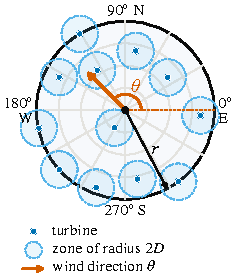
\includegraphics[width=\linewidth]{figures_final/fig_wind_farm.pdf}\\[-2pt]{\small (a)}
\end{minipage}\hfill
\begin{minipage}[b]{0.35\textwidth}\centering
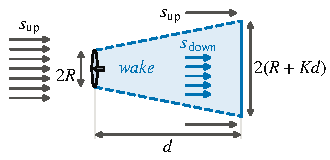
\includegraphics[width=\linewidth]{figures_final/fig_wake_model.pdf}\\[4pt]{\small (b)}
\end{minipage}\hfill
\begin{minipage}[b]{0.35\textwidth}\centering
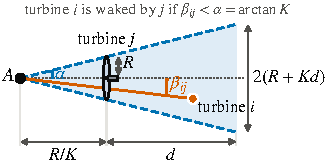
\includegraphics[width=\linewidth]{figures_final/fig_half_cone.pdf}\\[4pt]{\small (c)}
\end{minipage}
\caption{Model geometry. (a) Circular farm of radius $r$ and wind direction $\theta$; the points show, for illustration, a 12-turbine layout ($r=750$~m) of an earlier version of this study; discs of radius $2D$ touch at the spacing $\ell_{\min}=4D$. (b) Jensen top-hat wake behind a rotor of radius $R$: width $2(R+Kd)$ at the downstream distance $d$, uniform speed $s_{\text{down}}<s_{\text{up}}$. (c) Wake half cone of turbine $j$ ($K$ exaggerated): virtual vertex $A$ at $R/K$ upstream of the rotor, half-angle $\alpha=\arctan K$; turbine $i$ is waked by $j$ if $\beta_{ij}<\alpha$.}
\label{fig:model}
\label{fig:S-farm}\label{fig:S-wake}\label{fig:S-halfcone}
\end{figure}

\subsection{Wind Model and Direction Discretization}
\label{sec:wind}
For each direction, the wind speed $s$ has the Weibull density $p_s(s;\zeta,\psi)=(\zeta/\psi)\allowbreak(s/\psi)^{\zeta-1}\allowbreak\exp[-(s/\psi)^{\zeta}]$ with shape $\zeta(\theta)$ and scale $\psi(\theta)$. The benchmark rose is piecewise constant: $N_\theta=24$ direction bins $[15(l-1),15l)^\circ$, $l=1,\ldots,24$, with probability $p_l$, shape $\zeta=2$ and scale $\psi_l$ (Table~\ref{S-tab:S-wind}). Data Set~I is nearly unidirectional ($\psi=13$~m/s in all bins; 80\% of the probability in bins 6 and 7, i.e., wind from 165$^\circ$ to 195$^\circ$), Data Set~II is a broad rose with scales from 2.6 to 10~m/s and its highest probability in bin~13. The Horns Rev~1 block uses a measured 12-sector Weibull rose evaluated in 5$^\circ$ bins, and IEA37 Case Study~1 16 directions at one speed (Section~\ref{sec:setup-beyond}).
% verified: analysis/wflop_model.py (DS1_W, DS1_PSI, DS2_PSI, DS2_W; k = 2); bins 6+7 of DS I: 0.2+0.6 = 0.8, towards 75-105 deg = from 165-195 deg

\emph{Why the direction discretization matters.} The objective evaluates the wake only at the 24 bin centres $\bar\theta_l=15l-7.5^\circ$. A top-hat wake is narrow: by the half-cone geometry (Fig.~\ref{fig:model}c), turbine $j$ wakes a turbine $i$ at the distance $\rho\ge R/K$ only for directions within an interval of width $2[\alpha+\arcsin(R/(\rho\sqrt{1+K^2}))]$ around the direction from $j$ to $i$. With $K=0.075$ and $R=38.5$~m ($\alpha=4.29^\circ$, $R/K=513$~m), this width is below the bin spacing of 15$^\circ$ for $\rho>685$~m and tends to $2\alpha=8.6^\circ$. If no bin centre lies in this interval, the wake of the pair does not enter the objective (with bins of 5$^\circ$ or finer, every such interval contains a centre). Optimized layouts exploit these gaps: with 1$^\circ$ sub-bins that keep the Weibull parameters of their 15$^\circ$ bin, the mean wake loss of PSO-VNS rises from \NFLossPSOVNSFifteen\% to \NFLossPSOVNSOne\%, most for PSO and the VNS-based methods. All results thus hold for the discretized roses; Section~\ref{sec:robustness} reports which conclusions survive a 1$^\circ$ rose.
% verified (numerically with analysis/wflop_model.jensen_deficits on a 0.001-deg grid): waked width of a pair rho apart = 2(alpha + arcsin(R/(rho sqrt(1+K^2)))) exactly for rho >= R/K (rho = 600: 15.915 deg; 1000: 12.979; 2000: 10.779); width = 15 deg at rho = 685.4 m; alpha = arctan 0.075 = 4.289 deg; R/K = 513.3 m; 2 alpha = 8.58 deg > 5 deg. For rho < R/K the non-physical upstream deficit widens the interval further.
% CHECK-DIR [F03]: loss rise of every method, PSO-VNS 1.322 -> 2.335; [F05]: VNS-based methods and PSO rise most

\subsection{Wake Effect Model}
In the Jensen model (Fig.~\ref{fig:model}b,c), the wake of turbine $j$ is a half cone with half-angle $\alpha=\arctan K$ (wake-spreading constant $K$), and its virtual vertex lies $R/K$ upstream of the rotor. With $u_{ij}=(x_i - x_j)\cos\theta + (y_i - y_j)\sin\theta + R/K$ and the lateral offset $v_{ij}=-(x_i - x_j)\sin\theta + (y_i - y_j)\cos\theta$, turbine $i$ lies in the wake if $\beta_{ij}=\cos^{-1}\!\bigl(u_{ij}/\sqrt{u_{ij}^2+v_{ij}^2}\bigr)<\alpha$. Its downstream distance is $d_{ij}=\lvert u_{ij}-R/K\rvert$, and with the thrust coefficient $C_T$ the velocity deficit is
\begin{equation}
    \Delta_{ij} = 1-\frac{s_{\text{down}}}{s_{\text{up}}}=\frac{1 - \sqrt{1 - C_T}}{\left(1 + K d_{ij}/R\right)^2}.
    \label{eq:deficit}
\end{equation}
The numerator is the deficit behind the rotor from actuator-disc momentum theory, and the factor $R^2/(R+Kd_{ij})^2$ spreads it over the growing wake (Fig.~\ref{fig:model}b); with $C_T=0.8$ and $K=0.075$, a turbine $\ell_{\min}=308$~m directly behind another loses 21.6\% of the wind speed, one 770~m ($10D$) behind 8.8\%.
% verified: (1-sqrt(0.2))/(1+0.075*308/38.5)^2 = 0.2159; (1-sqrt(0.2))/(1+0.075*770/38.5)^2 = 0.0884
As in~\cite{Kusiak2010}, this top-hat wake is tested at the hub center only, so the deficit jumps at the cone edge, and it also reaches a turbine less than $R/K$ \emph{upstream} of $j$ near its axis (between $A$ and the rotor in Fig.~\ref{fig:model}c; non-physical, kept for comparability with the published results). The deficits are combined by the root-sum-square rule,
\begin{equation}\label{eq5}
\Delta_i(\theta) = \Bigl( \textstyle\sum_{j \ne i,\ \beta_{ij} < \alpha} \Delta_{ij}^2 \Bigr)^{1/2} .
\end{equation}
As $C_T$ is constant (which overstates the deficits above rated speed), the local wind speed in a direction bin is the free-stream speed times $1-\Delta_i(\theta)$, a Weibull variable with shape $\zeta(\theta)$ and scale $\psi_i(\theta)=\psi(\theta)[1-\Delta_i(\theta)]$. The hub-center test makes the objective jump where a hub crosses a cone edge in an evaluated direction; hence the derivative-free local search of VNS (Section~\ref{sec:vns}), and finite-difference gradients handicap MS-SLSQP.

\subsection{Power Model and Expected Energy}
\label{sec:powermodel}
\label{sec:S-power}
The power curve of the Kusiak--Song benchmark~\cite{Kusiak2010} is $f(s)=0$ for $s<s_{\text{cut-in}}$, $f(s)=\lambda_1 s+\lambda_0$ for $s_{\text{cut-in}}\le s\le s_{\text{rated}}$ and $f(s)=P_{\text{rated}}$ above, with $s_{\text{cut-in}}=3.5$~m/s, $s_{\text{rated}}=14$~m/s, $P_{\text{rated}}=1500$~kW, $\lambda_1=140.86$ and $\lambda_0=-500$. We use it as published: it is slightly negative just above the cut-in speed ($-7.0$~kW at 3.5~m/s, zero at 3.55~m/s), jumps from 1472 to 1500~kW at the rated speed and has no cut-out speed. The expected power of turbine $i$,
\begin{equation}\label{eq8}
E(P_i) = \int_0^{360} p_\theta(\theta) \int_0^{\infty} f(s)\,
       p_s\bigl(s; \zeta(\theta), \psi_i(\theta)\bigr) \, ds \, d\theta ,
\end{equation}
is evaluated, as in~\cite{Kusiak2010}, by a Riemann sum over direction bins $\theta_0 = 0^\circ, \theta_1, \ldots, \theta_{N_\theta} = 360^\circ$ with probabilities $p_l$, and the speed range between $s_{\text{cut-in}}$ and $s_{\text{rated}}$ into $N_s$ bins $s_0 = s_{\text{cut-in}}, s_1, \ldots, s_{N_s} = s_{\text{rated}}$ (benchmark: $N_\theta=24$ bins of 15$^\circ$ and $N_s=21$ bins of 0.5~m/s). With the bin centres $\bar\theta_l=(\theta_{l-1}+\theta_l)/2$ and the Weibull survival function $W_i(s,\theta)=\exp\{-[s/\psi_i(\theta)]^{\zeta(\theta)}\}$ of the local speed,
\begin{equation}
\begin{split}
E(P_i) ={}& \sum_{l=1}^{N_\theta} (\theta_l - \theta_{l-1})\, p_l \Bigg\{ P_{\text{rated}}\, W_i(s_{\text{rated}},\bar\theta_l)
+\lambda_1 \sum_{q=1}^{N_s} \tfrac{s_{q-1} + s_q}{2}\bigl[W_i(s_{q-1},\bar\theta_l)-W_i(s_q,\bar\theta_l)\bigr]\\
&\qquad+ \lambda_0 \bigl[W_i(s_{\text{cut-in}},\bar\theta_l)-W_i(s_{\text{rated}},\bar\theta_l)\bigr] \Bigg\}.
\end{split}
\label{eq:S-power}
\end{equation}
Like the earlier studies, we keep the bin-width factor $(\theta_l-\theta_{l-1})$ in degrees; with 24 bins of $15^\circ$ and $\sum_l p_l=1$, the benchmark objective $\sum_i E(P_i)$ is thus 15 times the expected farm power in kW, and the gross (wake-only) annual energy production is $\mathrm{AEP}\,[\mathrm{MWh}] = (\text{objective}/15)\times 8.76$. The wake-free benchmark objective of one turbine, $E_{\rm ideal}$, is~\eqref{eq:S-power} with $\psi_i=\psi$; for Data Set~I, $E_{\rm ideal}=14{,}045.74$, which corresponds to 936.38~kW (a capacity factor of 62\%, far above real sites) or 8,202.7~MWh/yr.
% verified: 14045.74/15 = 936.38 kW; 936.38/1500 = 0.624; 936.38*8.76 = 8202.7 MWh (R4 reproduced these from wflop_model.py); N_s = (14-3.5)/0.5 = 21 (wflop_model.expected_power_linear); 140.86*3.5-500 = -6.99; 500/140.86 = 3.55; 140.86*14-500 = 1472.0

\subsection{Optimization Problem and Constraint Handling}
\label{sec:constraints}
With the wake loss $L(\mathbf X)=N E_{\rm ideal}-\sum_{i=1}^{N}E(P_i)$, reported in percent of the wake-free value, $100\,L/(NE_{\rm ideal})$, the problem is
\begin{equation}
\min_{\mathbf X\in[-r,r]^{2N}} L(\mathbf X)\quad\text{s.t.}\quad \ell_{ij}\ge\ell_{\min}\ (1\le i<j\le N),\qquad x_i^2+y_i^2\le r^2\ (1\le i\le N),
\label{eq:wflop}
\end{equation}
which is equivalent to maximizing the expected farm power and hence the AEP: a problem in $2N$ variables ($2N\le30$ on the benchmark) with a discontinuous objective and $N(N-1)/2$ nonconvex spacing constraints.
After every position update, each coordinate is clipped to $[-r,r]$ (box repair; the square, not the circle). The constraints are handled by a penalty on the violations $g^{\rm b}_{i}=x_i^2+y_i^2-r^2$ and $g^{\rm s}_{ij}=\ell_{\min}-\ell_{ij}$; all optimizers except MS-SLSQP minimize the penalized wake loss
\begin{equation}
\begin{split}
F_p(\mathbf X)={}&\Bigl(N E_{\rm ideal}-\sum_{i=1}^{N}E(P_i)\Bigr)+\sum_{i:\,g^{\rm b}_i>0}\bigl(1+\mu g^{\rm b}_i\bigr)^2\\
&+\sum_{i<j:\,g^{\rm s}_{ij}>0}\bigl(1+\mu g^{\rm s}_{ij}\bigr)^2,\qquad \mu=10^{10},
\end{split}
\label{eq:penalty}
\end{equation}
whose first term is the wake loss $L(\mathbf X)$ reported in our tables. Any violation above about $4.6\cdot10^{-8}$ (m or m$^2$) makes the penalty exceed any possible wake loss, so comparing $F_p$ values is, up to smaller violations, a feasibility-first rule (feasible before infeasible, then wake loss or total penalty). The scaling ($g^{\rm b}_i$ in m$^2$, $g^{\rm s}_{ij}$ in m) favours infeasible layouts with turbines slightly too close, or with a turbine clipped to the box near a tangent point $(\pm r,y_i)$, where $g^{\rm b}_i=y_i^2$. MS-SLSQP minimizes the wake loss under explicit constraints. A final layout counts as feasible if $\ell_{ij}\ge\ell_{\min}$ and $\sqrt{x_i^2+y_i^2}\le r$ hold within $10^{-6}$~m (Section~\ref{sec:setup}), a looser tolerance than the penalty's.
% verified (R3-11): largest benchmark wake loss < 15 x 14045.74 = 2.107e5 (plus the small negative part of f); (sqrt(2.2e5)-1)/1e10 = 4.6e-8
% CHECK-DIAG [D06]/[D21]: old-setting infeasible finals (1e-6 m rule) mostly spacing-only; boundary violations = turbine with a coordinate on the box bound (tangent-point pinning); numbers in 06_results sec:psosetting
% <<<<< end optA/sw/03_model.tex
% >>>>> begin optA/sw/04_methods.tex
\section{Preliminaries: Phase-1 Methods and Basic VNS}
\label{sec:prelim}
% Proposition environment (neither IEEEtran nor elsarticle defines one); guarded, so a main file may define it in its preamble instead.
\makeatletter\@ifundefined{proposition}{\newtheorem{proposition}{Proposition}}{}\makeatother
A population method keeps $N_p$ candidate vectors $\mathbf X^i\in\mathbb R^{n}$ with components $X^i_m$ and bounds $lb_m=-r$, $ub_m=r$; unless stated otherwise, one iteration costs $N_p$ objective evaluations. This section states the methods exactly as implemented (Algorithms~\ref{alg:pso}--\ref{alg:vns}); Table~\ref{tab:params} collects all settings.

\subsection{PSO and Its Stability Conditions}
\label{sec:pso}
We use the canonical global-best PSO~\cite{Kennedy1995} in the inertia-weight form~\cite{Shi1998} (Algorithm~\ref{alg:pso}). Particle $i$ has a position $\mathbf X^i$, a velocity $\mathbf V^i$ and a personal best $\mathbf P^i$, the swarm keeps the global best $\mathbf G$, and a particle moves by
\begin{align}
\mathbf V^i&\leftarrow w\,\mathbf V^i+c_1\boldsymbol\rho_1\circ\bigl(\mathbf P^i-\mathbf X^i\bigr)+c_2\boldsymbol\rho_2\circ\bigl(\mathbf G-\mathbf X^i\bigr),\label{eq:pso-v}\\
\mathbf X^i&\leftarrow\mathbf X^i+\mathbf V^i,\label{eq:pso-x}
\end{align}
where $\boldsymbol\rho_1,\boldsymbol\rho_2$ are vectors of independent $U(0,1)$ numbers, drawn anew for every move, and $\circ$ is the componentwise product. The constriction PSO of Clerc and Kennedy~\cite{Clerc2002} with their standard choice $\varphi_1=\varphi_2=2.05$ (constriction factor $\kappa=0.7298$) is identical to \eqref{eq:pso-v} with
\begin{equation}
w=0.7298,\qquad c_1=c_2=\kappa\varphi_1=1.49618 .
\label{eq:constriction}
\end{equation}
PSO denotes \eqref{eq:pso-v}, \eqref{eq:pso-x} with these coefficients, fixed a priori from the literature, and the \emph{old setting} the same algorithm with $w=0.7$, $c_1=c_2=2$, i.e., the acceleration coefficients of the original PSO~\cite{Kennedy1995} combined with an inertia weight. Both are run as implemented: velocities start at zero and are not clamped (no $V_{\max}$), a coordinate clipped to the square (Section~\ref{sec:constraints}) keeps its velocity, and $\mathbf P^i$, $\mathbf G$ are updated after each evaluation (asynchronous global best).

\begin{algorithm}[!t]
\caption{PSO as implemented ($N_p(T+1)$ evaluations)}
\label{alg:pso}
\small
\begin{algorithmic}[1]
\State Draw (seeded) and evaluate $N_p$ layouts $\mathbf X^i$; $\mathbf V^i\gets\mathbf 0$, $\mathbf P^i\gets\mathbf X^i$, $\mathbf G\gets\arg\min_i F_p(\mathbf P^i)$
\For{$t=1,\ldots,T$ and $i=1,\ldots,N_p$}
    \State Draw $\boldsymbol\rho_1,\boldsymbol\rho_2\sim U(0,1)^n$; update $\mathbf V^i$ by \eqref{eq:pso-v} \Comment{no velocity clamping}
    \State $\mathbf X^i\gets\operatorname{clip}(\mathbf X^i+\mathbf V^i,-r,r)$ \Comment{box repair; $\mathbf V^i$ is kept}
    \State Evaluate $F_p(\mathbf X^i)$; replace $\mathbf P^i$ and $\mathbf G$ if it is strictly lower than theirs
\EndFor
\State \Return $\mathbf G$
\end{algorithmic}
\end{algorithm}

\emph{Stability under stagnation.} Consider one coordinate $x=X^i_m$ with $v=V^i_m$, $p=P^i_m$ and $g=G_m$, and assume (A1) \emph{stagnation}, $p$ and $g$ fixed, and (A2) \emph{no active bound}, so that $v_t=x_t-x_{t-1}$. With $\varphi_{k,t}=c_k\rho_{k,t}$ and $\varphi_t=\varphi_{1,t}+\varphi_{2,t}$, every coordinate then follows the random linear recursion $x_{t+1}=(1+w-\varphi_t)\,x_t-w\,x_{t-1}+\varphi_{1,t}\,p+\varphi_{2,t}\,g$, whose random coefficient $\varphi_t$ has mean $\mu=(c_1+c_2)/2$ and variance $\sigma^2=(c_1^2+c_2^2)/12$. The update is \emph{order-1} (\emph{order-2}) \emph{stable} if $\mathrm E\,x_t$ (and $\mathrm E\,x_t^2$) converges to a limit independent of $(x_0,x_1)$~\cite{Poli2009}.

\begin{proposition}\label{prop:pso-stability}
Let $c_1,c_2\ge0$, $c_1+c_2>0$, and assume (A1)--(A2).
\begin{enumerate}
\item[(a)] $\mathrm E\,x_t\to x^*=(c_1p+c_2g)/(c_1+c_2)$ for all initial values if and only if $\lvert w\rvert<1$ and $0<c_1+c_2<4(1+w)$.
\item[(b)] The update is order-2 stable if and only if $\lvert w\rvert<1$ and
\begin{equation}
\chi(1):=2\mu(1-w^2)-(1-w)\mu^2-(1+w)\sigma^2>0 .
\label{eq:pso-o2}
\end{equation}
For $c_1=c_2$, \eqref{eq:pso-o2} is Poli's condition~\cite{Poli2009}
\begin{equation}
c_1+c_2<\frac{24\,(1-w^2)}{7-5w};
\label{eq:poli}
\end{equation}
for $c_1\ne c_2$ with the same sum $c_1+c_2$, it is stricter.
\item[(c)] Under (b), $\operatorname{Var}x_t\to V_\infty=(1+w)\,q/\chi(1)$ with $q=c_1^2c_2^2(p-g)^2/[6(c_1+c_2)^2]$, for $c_1=c_2=c$ $V_\infty=c(1+w)(p-g)^2/(4[12(1-w^2)-c(7-5w)])$; $V_\infty=0$ if and only if $p=g$.
\end{enumerate}
\end{proposition}
\begin{proof}[Proof sketch]
(a) $e_t=\mathrm E\,x_t-x^*$ obeys $e_{t+1}=(1+w-\mu)\,e_t-w\,e_{t-1}$; both roots of $\lambda^2-(1+w-\mu)\lambda+w$ lie strictly inside the unit circle if and only if $\lvert w\rvert<1$ and $\lvert 1+w-\mu\rvert<1+w$ (Schur--Cohn), i.e., $0<\mu<2(1+w)$. (b) With $y_t=x_t-x^*$, $z_t=(\mathrm Ey_t^2,\mathrm Ey_ty_{t-1},\mathrm Ey_{t-1}^2)^{\mathsf T}$ obeys $z_{t+1}=Mz_t+b_t$ with a $3\times3$ matrix $M(w,\mu,\sigma^2)$ and $b_t\to(q,0,0)^{\mathsf T}$, so order-2 stability means a spectral radius of $M$ below one; by Jury's criterion for its characteristic polynomial $\chi$, this holds iff $\lvert w\rvert<1$ and $\chi(1)>0$. For $c_1=c_2=c$, $\chi(1)=c\,[12(1-w^2)-c(7-5w)]/6$; for fixed $c_1+c_2$, $\sigma^2$ is smallest at $c_1=c_2$. (c) $V_\infty$ is the first component of the fixed point of $z\mapsto Mz+(q,0,0)^{\mathsf T}$. Full proof: Section~\ref{S-sec:S-th-pso}.
\end{proof}
The order-1 condition involves the \emph{mean} of $\varphi_t$ (with $\varphi=c_1+c_2$, the constant-coefficient condition $\varphi<2(1+w)$ would wrongly call the old setting unstable). For $c_1=c_2$, the region also holds under a weaker, non-stagnant assumption~\cite{Cleghorn2018}. The constriction setting is order-2 stable ($c_1+c_2=2.99<3.35$; spectral radius of $M$ 0.94): in the limit, a coordinate with $P^i_m\ne G_m$ is sampled with mean $(P^i_m+G_m)/2$ and standard deviation $1.04\,\lvert P^i_m-G_m\rvert$, so the swarm keeps sampling around $\mathbf G$ unless $\mathbf P^i=\mathbf G$. The old setting is order-1 stable ($4<6.8$) but beyond the order-2 boundary ($4>3.50$; $c_1=c_2>c^*=\NSBoundC$ at $w=0.7$; spectral radius 1.12), so its second moments grow without bound under stagnation (Fig.~\ref{fig:S-th-stability}; Proposition~\ref{S-prop:S-settings}). Neither condition says how good $\mathbf G$ is, and clipping violates (A2): a clipped coordinate stays at the bound while its kept velocity points outward (Lemma~\ref{S-lem:S-clip}).
\begin{figure}[!t]
\begin{minipage}[c]{0.44\textwidth}\centering
\pipefig{\linewidth}{figures_mpce/theory_stability.pdf}{6cm}
\end{minipage}\hfill
\begin{minipage}[c]{0.53\textwidth}
\caption{Stability regions of the implemented PSO update under stagnation and without active bounds ($c_1=c_2$; Proposition~\ref{prop:pso-stability}). Light: order-1 stable only, $c_1+c_2<4(1+w)$; dark: order-1 and order-2 stable, $c_1+c_2<24(1-w^2)/(7-5w)$. The old setting ($w=0.7$, $c_1=c_2=2$) is order-1 but not order-2 stable; the constriction setting~\eqref{eq:constriction} is order-2 stable.}
\label{fig:S-th-stability}
\end{minipage}
\end{figure}
% CHECK-THEORY [T01]-[T06], [T12]: Proposition prop:pso-stability (full statement of S-prop:S-pso-stability, whose full proof stays in the supplement; order-1 via E[phi]=(c1+c2)/2; Poli's bound exact for c1=c2, analytic region = numerical region, T06); 24(1-0.7^2)/(7-3.5)=3.497; 24(1-0.7298^2)/(7-5*0.7298)=3.348; 4(1+0.7)=6.8; 2*1.49618=2.99; spectral radius of the second-moment matrix 1.124 (old) and 0.944 (constriction) in Table S-th-settings; c* = 3.497/2 = \NSBoundC
% CHECK-THEORY [T05]: SD factor 1.04 = sqrt(V_inf/(p-g)^2) = sqrt(1.0874) (constriction); constant-coefficient misclassification 2(1+0.7) = 3.4 (S-th-pso note); Lemma S-lem:S-clip (b): clipped coordinate stays at the bound while v' >= 0
Section~\ref{sec:psosetting} tests this empirically: in a sweep of $c_1=c_2=c$ at $w=0.7$, feasibility starts to fall near $c^*$ and falls progressively beyond it (to \NSFeasCTwoZero\% at $c=2$), so the boundary marks approximately where this PSO starts to fail, and velocity clamping largely rescues the old setting. DE's $F=0.5$ exceeds Zaharie's critical value (0.14 at $\mathrm{CR}=0.9$)~\cite{Zaharie2002}, so its weak results are not due to premature variance loss.
% verified (Zaharie): critical F = sqrt((1-CR/2)/N_p) = sqrt((1-0.45)/30)=0.135 (N_p = 30, CR = 0.9, F = 0.5: Section setup); F above the critical value = no variance collapse (R3-10, R1-15); Cleghorn2018 cited for c1 = c2 only (R3-14)
% CHECK-CSWEEP [S02]-[S05]: feasibility >= 98 % for c <= 1.7, falls progressively beyond c* = \NSBoundC (\NSFeasCOneEight > \NSFeasCOneNine > \NSFeasCTwoZero at c = 1.8, 1.9, 2.0), onset in the step containing c* ("starts to fall near c*", "marks approximately where ... starts to fail"); [S10]/[S11]: vmax = \NSVmaxFrac (ub-lb) >= 90 % feasible but still worse than constriction ("largely rescues"); details in 06_results
% CHECK-DIAG [D03]/[D06]/[D21]: the diagnostics of the old setting (contraction, spacing-only finals, tangent-point pinning) are stated in 06_results (sec:psosetting), no longer here

\subsection{Salp Swarm Algorithm and Its Laplacian Variant}
\label{sec:ssa}
\label{sec:S-ssa}
The SSA~\cite{Mirjalili2017} (Algorithm~\ref{S-alg:S-ssa}) keeps the best solution found so far as the food source $\mathbf H$ and splits the population, sorted by $F_p$, into leaders and followers. A leader $i\le N_p/2$ updates each coordinate by
\begin{equation}\label{eq:leader}
X_m^i = H_m\pm\xi_1\big((ub_m-lb_m)\xi_2+lb_m\big),
\end{equation}
with either sign with probability $1/2$, $\xi_2\sim U(0,1)$ and $\xi_1=2\exp[-(4t/T)^2]$ decreasing with the iteration $t$ out of $T$: a leader samples $H_m+U(-\xi_1r,\xi_1r)$ in every coordinate, with $\xi_1\le0.037$ for $t\ge T/2$. A follower $i>N_p/2$ moves to the midpoint of its position and the \emph{new} position of the preceding salp. The leaders thus perturb $\mathbf H$ uniformly with a shrinking radius, and the followers only average~\cite{Castelli2022}. LX-SSA~\cite{Solanki2023} gives each follower a second candidate $Y_m^i=X_m^i+\gamma(H_m-X_m^i)$ with one Laplace step~\cite{Deep2007} for all coordinates,
\begin{equation}
\gamma=\phi-\chi\,\mathrm{sgn}\bigl(z-\tfrac12\bigr)\ln\bigl(1-2\lvert z-\tfrac12\rvert\bigr),\quad z\sim U(0,1),
\label{eq:laplace}
\end{equation}
$\phi=0$, $\chi=1$, and keeps the better candidate. As published, it evaluates both candidates of each follower and then re-evaluates the kept ones with the new population, so an iteration costs $2N_p$ evaluations (SSA: $N_p$) and LX-SSA runs half as many iterations as SSA (Table~\ref{tab:params}). Comparing the two tests LX-SSA as published, not the Laplace step alone; both use the code of the previous study.
% CHECK-THEORY [T11]: SSA xi_1(T/2) = 2 exp(-4) = 0.0366 ("xi_1 <= 0.037 for t >= T/2"); leader step xi_1((ub-lb) xi_2 + lb) = xi_1 r (2 xi_2 - 1) (S-th-feas note)
% verified: analysis/authors_optimizers.py SSA/LXSSA: leaders = pop_size // 2 = 15; follower = (pop[i] + new_pop[i-1])/2; LX: one scalar gamma per follower, candidate = pop[i] + gamma (food - pop[i]); both clipped and evaluated, then whole population evaluated (2 N_p per iteration)

% Page budget: the SSA/LX-SSA pseudocode stays in the supplementary material (Algorithm S-alg:S-ssa); main-text version was:
% \begin{algorithm}[!t]
% \caption{SSA and LX-SSA (LX: LX-SSA only; evaluations in brackets)}
% \label{alg:S-ssa}
% \small
% \begin{algorithmic}[1]
% \State Draw and evaluate $N_p$ salps; sort them by $F_p$ and set the best as food source $\mathbf H$. \Comment{[$N_p$]}
% \For{$t=1$ to $T$}
%     \State Update $\xi_1=2\exp[-(4t/T)^2]$.
%     \State Leaders $i\le N_p/2$: new position $\tilde{\mathbf X}^i$ by \eqref{eq:leader}.
%     \For{followers $i=N_p/2+1,\ldots,N_p$}
%         \State $\tilde{\mathbf X}^i\gets\mathbf Z^i=\tfrac{1}{2}(\mathbf X^i+\tilde{\mathbf X}^{i-1})$
%         \State LX: form $\mathbf Y^i$ by \eqref{eq:laplace}, box-repair $\mathbf Y^i$ and $\mathbf Z^i$, evaluate both, $\tilde{\mathbf X}^i\gets$ the better \Comment{[2 per follower]}
%     \EndFor
%     \State Box-repair $\tilde{\mathbf X}$, set $\mathbf X\gets\tilde{\mathbf X}$, evaluate $F_p$ for all salps, sort them, and update $\mathbf H$. \Comment{[$N_p$]}
% \EndFor
% \State \Return $\mathbf H$.
% \end{algorithmic}
% \end{algorithm}

\subsection{Basic Variable Neighborhood Search}
\label{sec:vns}
The basic VNS~\cite{Mladenovic1997,Hansen2001}, in the continuous form of~\cite{Mladenovic2008} (Algorithm~\ref{alg:vns}), improves one incumbent $\mathbf X$ with $k_{\max}=5$ nested $\ell_\infty$ neighborhoods $\mathcal N_k(\mathbf X)=\{\mathbf X':\delta_{k-1}<\lVert \mathbf X'-\mathbf X\rVert_\infty\le\delta_k\}$, $\delta_k=0.1\,k\,r$, of the whole layout: shaking draws a uniform point of $\mathcal N_k(\mathbf X)$, clipped to the box, and a best-improvement local search improves it. As the top-hat wake makes $F_p$ discontinuous, the local search is a compass search: it evaluates all $2n$ moves $\pm h\,\mathbf e_m$ ($\mathbf e_m$ the $m$th unit vector; 60 evaluations for $N=15$), moves to the best one if it strictly improves, and halves $h$ (from $h_0=0.05r$) when none does, until $h<h_{\min}=10^{-3}r$. A completed descent ends at a point that no move $\pm\bar h\,\mathbf e_m$, $\bar h=h_0/2^5=0.0015625\,r$, improves (Proposition~\ref{S-prop:S-ls}), a coordinate-wise optimality at one step length, not a local minimum.
% CHECK-THEORY [T12]: compass search final step h0/2^5 = 0.0015625 r (Proposition S-prop:S-ls); verified: analysis/original_vns.py (k_max = 5, rho_k = 0.1 k r, h0 = 0.05 r, h_min = 1e-3 r; move to the best of the 2 dim moves if it improves the current point, else halve h; shaking by rejection in the l_inf shell, then clip)

\begin{algorithm}[!t]
\caption{Basic VNS from an incumbent $\mathbf X$ (until the budget is used; returns the best layout evaluated)}
\label{alg:vns}
\small
\begin{algorithmic}[1]
\State $\mathbf X\gets\textsc{LocalSearch}(\mathbf X)$; $k\gets1$
\Loop
    \State Draw $\mathbf d\sim U[-\delta_k,\delta_k]^n$ until $\lVert\mathbf d\rVert_\infty>\delta_{k-1}$; evaluate $\mathbf X'=\operatorname{clip}(\mathbf X+\mathbf d)$ \Comment{shaking}
    \State $\mathbf X'\gets\textsc{LocalSearch}(\mathbf X')$; \textbf{if} $F_p(\mathbf X')<F_p(\mathbf X)$ \textbf{then} $\mathbf X\gets\mathbf X'$, $k\gets1$ \textbf{else} $k\gets k\bmod k_{\max}+1$
\EndLoop
\Function{LocalSearch}{$\mathbf y$} \Comment{compass search, best improvement}
    \State $h\gets h_0$; \textbf{while} $h\ge h_{\min}$: evaluate the $2n$ points $\operatorname{clip}(\mathbf y\pm h\,\mathbf e_m)$; if the best, $\mathbf y'$, has $F_p(\mathbf y')<F_p(\mathbf y)$, then $\mathbf y\gets\mathbf y'$, else $h\gets h/2$
    \State \Return $\mathbf y$
\EndFunction
\end{algorithmic}
\end{algorithm}

\section{Two-Phase Swarm--VNS Design and PSO-VNS}
\label{sec:hybrid}

\subsection{Two-Phase Template}
\label{sec:template}
All hybrids follow one sequential (relay) template. For a budget of $B$ evaluations and a split $\omega\in(0,1)$, Phase~1 starts from the seeded initial population, runs a population method for about $\omega B$ evaluations and passes its best layout to Phase~2, the basic VNS (Algorithm~\ref{alg:vns}), which applies the local search to it and then iterates until $B$ evaluations are used. Only Phase~1 differs: PSO in \emph{PSO-VNS}; SSA or LX-SSA in \emph{SSA-VNS} and \emph{LX-SSA-VNS} (with $\xi_1$ compressed to the Phase-1 iterations); and, in the controls, $\operatorname{round}(\omega B)$ layouts: the initial population, then layouts drawn uniformly in the farm disc (\emph{RSD-VNS}) or in its bounding square (\emph{RS-VNS}). VNS alone is the limiting case in which Phase~1 is the initial population. Phase~1 runs for $T_1=\operatorname{round}((\omega B-N_p)/c)$ iterations of $c$ evaluations ($c=N_p$ for PSO and SSA, $2N_p$ for LX-SSA). A swarm phase is useful only if it gives VNS a better start than random sampling with about the same number of evaluations (at $\omega=0.5$, 3,015 for the controls and $N_p(T_1+1)=3{,}030$ for the swarms); the component analysis (Section~\ref{sec:ablation}) tests this for each Phase-1 choice against RSD-VNS, with RS-VNS as a weak minimum bar, as the following result shows.

\begin{proposition}\label{prop:S-box}
Let the $2N$ coordinates be independent and uniform in $[-r,r]$, and let $P_N$ be the probability that the layout is feasible (all turbines in the disc $\mathcal D$ of radius $r$ and all pairwise distances $\ge s$). Then (a) all $N$ turbines lie in $\mathcal D$ with probability $(\pi/4)^N$; (b) $P_N\le(\pi/4)^N\prod_{k=1}^{N-1}\max\bigl\{0,\ 1-\max\{A(s),\,k\,A(s/2)\}/(\pi r^2)\bigr\}$, where $A(\rho)$ is the area of the part of $\mathcal D$ covered by a disc of radius $\rho$ centred on the boundary of $\mathcal D$ (closed form: \eqref{S-eq:S-th-lens}); (c) among $M$ such layouts, the expected number of feasible ones is $MP_N$.
\end{proposition}
\begin{proof}
(a) The turbines are independent and uniform in the square, each in $\mathcal D$ with probability $\pi r^2/(2r)^2$. (b) Given (a), the positions $\mathbf p_1,\ldots,\mathbf p_N$ are independent and uniform in $\mathcal D$. If $\mathbf p_1,\ldots,\mathbf p_k$ are pairwise at least $s$ apart, $\mathbf p_{k+1}$ must avoid $U_k=\mathcal D\cap\bigcup_{j\le k}B(\mathbf p_j,s)$. The area of $B(\mathbf c,\rho)\cap \mathcal D$, $\mathbf c\in \mathcal D$, is nonincreasing in $\lVert\mathbf c\rVert$ (its derivative is minus the length of the common chord), hence $\ge A(\rho)$; so $\lvert U_k\rvert\ge A(s)$, and, as the discs $B(\mathbf p_j,s/2)\subset B(\mathbf p_j,s)$ are disjoint, $\lvert U_k\rvert\ge kA(s/2)$. The chain rule over $k$ gives (b). (c) Linearity of expectation.
\end{proof}
The bound (b) is loose; by Monte Carlo, $P_N<10^{-6}$ for the largest cases ($N=12$, 15; $N=10$: no feasible layout in $10^7$), so the 3,015 samples of RS-VNS contain about $10^{-3}$ or fewer feasible layouts in expectation (Table~\ref{S-tab:S-th-box}), and RS-VNS hands VNS the least-violating sample. The spacing dominates ($P_N\ll(\pi/4)^N$): \NRSRunsNoFeasSample{} RS-VNS runs have no feasible sample, and disc sampling gives one in only \NRsSquareExplains{} of them.
% CHECK-THEORY [T07]-[T10]: Proposition prop:S-box (= S-prop:S-box, restored in the main text with its proof; R1-6 had moved it to the supplement): (pi/4)^N, rigorous spacing bound (lens area nonincreasing, T10), Monte Carlo P_N < 1e-6 for N = 12, 15 (N = 10: 0 of 1e7), expected feasible of 3,015 <= 1.0e-3 (Table S-tab:S-th-box)
% CHECK-DIAG [D17]: RS-VNS Phase-1 replay agrees with the runs and with (pi/4)^N; \NDRsRunsNoFeasSample (= \NRSRunsNoFeasSample) runs without any feasible Phase-1 sample
% CHECK-FINAL [C60]: spacing binding (R3-6): of the \NRSRunsNoFeasSample RS-VNS runs without a feasible sample, disc sampling (RSD-VNS, same runs) rescues \NRsSquareExplains < \NRsSpacingDominates that stay without one ("mainly because of the spacing"); [C61]: controls switch at 3,015, swarms at 3,030; RSD-VNS definition: mpce_experiments.RSDVNS (first 30 = common initial population, then polar-uniform disc samples)

\subsection{PSO-VNS}
PSO-VNS (Algorithm~\ref{alg:hybrid}) is not a new PSO variant: its Phase~1 is the plain PSO of Algorithm~\ref{alg:pso} and, as the coefficients do not depend on the iteration, reproduces exactly, for a given seed, the first $N_p(T_1+1)$ evaluations of a PSO run (Proposition~\ref{S-prop:S-prefix}); comparing PSO-VNS with PSO thus isolates the effect of Phase~2. This does not hold for SSA-VNS and LX-SSA-VNS, whose $\xi_1$ depends on $t/T_1$.

\begin{algorithm}[!t]
\caption{PSO-VNS for a prescribed turbine count $N$}
\label{alg:hybrid}
\small
\begin{algorithmic}[1]
\Require budget $B$, split $\omega$, $N_p$, $w$, $c_1$, $c_2$, radius $r$, $k_{\max}$
\State $\mathbf G\gets$ PSO (Algorithm~\ref{alg:pso}) with $T=T_1=\operatorname{round}((\omega B-N_p)/N_p)$ \Comment{Phase 1}
\State $\mathbf X\gets\textsc{LocalSearch}(\mathbf G)$; $k\gets1$ \Comment{Phase 2 (Algorithm~\ref{alg:vns})}
\While{fewer than $B$ evaluations have been used}
    \State $\mathbf X'\gets\textsc{LocalSearch}(\text{uniform point of }\mathcal N_k(\mathbf X))$; \textbf{if} $F_p(\mathbf X')<F_p(\mathbf X)$ \textbf{then} $\mathbf X\gets \mathbf X'$, $k\gets1$ \textbf{else} $k\gets k\bmod k_{\max}+1$
\EndWhile
\State \Return best layout evaluated
\end{algorithmic}
\end{algorithm}


PSO-VNS adds one parameter to PSO and VNS, the split $\omega$; with $\omega=0.5$ and $B=6{,}030$, PSO runs for $T_1=100$ iterations (99.5 rounded half to even) and VNS receives 3,000 evaluations (Table~\ref{tab:params}). None of these values was tuned; Section~\ref{sec:split} studies $\omega$. At this budget, PSO-VNS is essentially PSO plus one compass-search descent: the first descent is unfinished in \NDDescentUnfinishedLargePSOVNS{} of \NDRunsLargePSOVNS{} runs with $N\ge12$, and shaking-plus-search cycles take \NDCycleEvalsPctPSOVNS\% of the Phase-2 evaluations (pooled; median run \NDCycleEvalsPctMedianPSOVNS\%) for \NDCycleSharePSOVNS\% of the Phase-2 gain (accepted cycles), so the neighborhoods matter only for small $N$.
% CHECK-DIAG [D08]: essentially one compass-search descent (median shaking steps \NDShakesPSOVNS, first descent \NDDescentSharePSOVNS % of the Phase-2 improvement; 12 split cases x 10 seeds; same pattern for SSA-VNS, RS-VNS); [D20]: cycles \NDCycleEvalsPctPSOVNS % of the Phase-2 evaluations pooled (median run \NDCycleEvalsPctMedianPSOVNS %), accepted cycles \NDCycleSharePSOVNS % of the gain (\NDCycleAllSharePSOVNS % incl. the cycle cut off by the budget)
% CHECK-DIAG [D09]: N >= 12: first descent unfinished in \NDDescentUnfinishedLargePSOVNS of \NDRunsLargePSOVNS runs, median run without shaking ("neighborhoods matter only for small N")
% verified (R3-16): Python round(99.5) = 100 (half to even); omega = 0.25/0.75/0.9 give 49/150/180

Table~\ref{tab:params} lists the settings of all methods, the published defaults~\cite{Clerc2002,Mirjalili2017,Solanki2023,Storn1997,Mladenovic2008}; MS-SLSQP (SciPy's SLSQP~\cite{Kraft1988}) minimizes $L$ under the scaled constraints of~\eqref{eq:wflop} (Section~\ref{S-sec:S-slsqp}). At 30,030 and 120,030 evaluations (Section~\ref{sec:budget}), $T$ and $T_1$ follow the same rules.
\begin{table}[!t]
\centering
\caption{Settings of all methods at the benchmark budget $B=6{,}030$ evaluations (including the initial population and, for MS-SLSQP, the finite-difference calls); $N_p=30$; box repair by clipping to $[-r,r]$. A population method uses $N_p(T+1)$ evaluations, LX-SSA $N_p(2T+1)$.}
\label{tab:params}
\scriptsize\setlength{\tabcolsep}{3.5pt}
\begin{tabular}{@{}>{\raggedright\arraybackslash}p{0.14\textwidth}>{\raggedright\arraybackslash}p{0.14\textwidth}>{\raggedright\arraybackslash}p{0.68\textwidth}@{}}
\toprule
Method & Iterations & Coefficients and operators \\
\midrule
PSO & $T=200$ & Algorithm~\ref{alg:pso}; $w=0.7298$, $c_1=c_2=1.49618$ (old setting: $w=0.7$, $c_1=c_2=2$); $\mathbf V^i_0=\mathbf 0$, no $V_{\max}$; clipped coordinate keeps its velocity; asynchronous $\mathbf P^i$, $\mathbf G$ \\
SSA & $T=200$ & Algorithm~\ref{S-alg:S-ssa}; 15 leaders, 15 followers; $\xi_1=2\exp[-(4t/T)^2]$ \\
LX-SSA & $T=100$ & as SSA, plus a Laplace candidate per follower, $\phi=0$, $\chi=1$~\eqref{eq:laplace}; both candidates evaluated \\
DE/rand/1/bin & $T=200$ & $F=0.5$, $\mathrm{CR}=0.9$; mutant clipped before crossover; asynchronous one-to-one replacement \\
VNS & 30 initial, then 6,000 & Algorithm~\ref{alg:vns} from the best initial layout; $k_{\max}=5$, $\delta_k=0.1kr$, $h_0=0.05r$, $h_{\min}=10^{-3}r$ \\
MS-SLSQP & $\le200$ per start & SLSQP, $\mathrm{ftol}=10^{-9}$, forward differences (step 1~m); starts: initial layouts by increasing $F_p$, then random layouts \\
PSO-VNS, SSA-VNS, LX-SSA-VNS & $T_1=100$ / 100 / 50 (3,030), then 3,000 & $\omega=0.5$; Phase~1 PSO / SSA / LX-SSA as above ($\xi_1$ over $T_1$), Phase~2 VNS (Algorithm~\ref{alg:hybrid}) \\
RS-VNS, RSD-VNS & 3,015 samples, then 3,015 & $\omega=0.5$; initial population, then uniform layouts in the square / disc; Phase~2 VNS \\
\bottomrule
\end{tabular}
\end{table}
% verified: analysis/authors_optimizers.py (PSO, DE, SSA, LXSSA), analysis/original_vns.py (BVNS defaults), analysis/hybrid_lxssa_bvns.py (T1 = round((split B - Np)/per_iter)), supplement sec:S-iter and sec:S-slsqp (MS-SLSQP: maxiter 200 per start, ftol 1e-9, eps 1 m, scaled constraints, feasibility threshold -1e-9)
% <<<<< end optA/sw/04_methods.tex
% >>>>> begin optA/sw/05_setup.tex
\section{Evaluation Protocol}
\label{sec:setup}

\subsection{Cases and Methods}
\label{sec:setup-cases}
The 68 cases combine the two Kusiak--Song wind data sets~\cite{Kusiak2010,Bansal2017} (Table~\ref{S-tab:S-wind}) with circular farms of radii $r=500$, 750 and 1000~m and $N=2,\ldots,10$, $2,\ldots,12$ and $2,\ldots,15$ turbines ($R=38.5$~m, $\ell_{\min}=4D=308$~m, $C_T=0.8$, $K=0.075$).

The \emph{main comparison} includes eight methods ($N_p=30$ where applicable): PSO-VNS (Algorithm~\ref{alg:hybrid}, $\omega=0.5$); PSO; SSA-VNS; SSA; LX-SSA; DE/rand/1/bin~\cite{Storn1997} (scale factor 0.5, crossover rate 0.9); VNS; and MS-SLSQP, a multistart sequential least-squares programming method (SciPy's SLSQP~\cite{Kraft1988}, forward-difference gradients) that minimizes the wake loss under explicit constraints, restarting from the initial, then random layouts (Section~\ref{S-sec:S-protocol}); all others minimize $F_p$~\eqref{eq:penalty} over $[-r,r]^{2N}$. The \emph{component analysis} (Section~\ref{sec:ablation}) adds LX-SSA-VNS and two random-sampling controls (Section~\ref{sec:template}; RSD-VNS on the benchmark only): after the common initial population, \emph{RSD-VNS} samples Phase~1 uniformly in the farm disc and \emph{RS-VNS} in the bounding square, 3,015 layouts versus the hybrids' 3,030 Phase-1 evaluations. A split study varies $\omega$ on \NSplitCases{} cases (Section~\ref{sec:split}). Table~\ref{tab:design} lists all studies of the paper with their cases, methods, budgets, seeds and runs; the re-evaluations and diagnostics use stored layouts and runs.
% CHECK-FINAL [C61]: RS-VNS and RSD-VNS switch after round(0.5 x 6,030) = 3,015 Phase-1 evaluations; RSD-VNS = experiment rsdisc (68 cases x 30 seeds only; not in the budget, feasible-start, Horns Rev or IEA37 studies); CHECK-DIAG [D17]: RS-VNS Phase-1 replay

\begin{table}[!htbp]
\centering
\caption{Experimental design. Budget: objective evaluations per run, all counted (initial population, finite-difference evaluations of MS-SLSQP); r: random, f: feasibility-preserving initialization. Runs: new optimization runs (``reused'': taken from another study). Ten methods: the eight of the main comparison, LX-SSA-VNS and RS-VNS. Split cases: middle and largest $N$ per farm and data set; six largest: largest $N$ per farm and data set. In total, 36{,}190 optimization runs.}
\label{tab:design}
\scriptsize
\setlength{\tabcolsep}{3pt}
\begin{tabular}{@{}>{\raggedright\arraybackslash}p{2.0cm}>{\raggedright\arraybackslash}p{1.85cm}>{\raggedright\arraybackslash}p{5.6cm}>{\raggedright\arraybackslash}p{2.15cm}>{\raggedright\arraybackslash}p{1.05cm}>{\raggedright\arraybackslash}p{1.15cm}>{\raggedright\arraybackslash}p{0.55cm}@{}}
\toprule
Study & Cases & Methods & Budget (init.) & Seeds & Runs & Sec. \\
\midrule
Main comparison & 68 benchmark & PSO-VNS, PSO, SSA-VNS, SSA, LX-SSA, DE, VNS, MS-SLSQP & 6,030 (r) & 1--30 & \NRunsMain & \ref{sec:overall} \\
Component analysis & 68 & LX-SSA-VNS, RS-VNS, RSD-VNS (\NDRsDiscRuns{} each); six reused & 6,030 (r) & 1--30 & 6{,}120 & \ref{sec:ablation} \\
Old PSO setting & 68 & PSO, $w=0.7$, $c_1=c_2=2$ & 6,030 (r) & 1--30 & \NDStoredRunsOld & \ref{sec:psosetting} \\
Budget split & \NSCases{} split cases & PSO-VNS, $\omega=0.25$, 0.75, 0.9 (\NDOmegaNinetyRuns{} each); $\omega=0.5$, 1 reused & 6,030 (r) & 1--30 & 1{,}080 & \ref{sec:split} \\
Coefficient sweep & \NSCases{} split cases & PSO, $w=0.7$, $c_1=c_2=c=1.2$, 1.4, 1.6--2.0 (step 0.1); $c=2$ with $v\gets0$ or $\lvert v\rvert\le\NSVmaxFrac\,(u-l)$ (\NSRuns{} each) & 6,030 (r) & 1--30 & 3{,}240 & \ref{sec:psosetting} \\
Budget scaling & six largest & ten methods (6,030 reused) & 30,030; 120,030 (r) & 1--30 & 3{,}600 & \ref{sec:budget} \\
Feasible starts & six largest & ten methods except RS-VNS & 6,030 (f) & 1--30 & 1{,}620 & \ref{sec:feasinit} \\
Horns Rev~1 & 16 turbines & ten methods (f: except RS-VNS) & 6,030 (r, f); 30,030, 120,030 (r) & 1--30; 1--10 at 120,030 & \NFHRNRuns & \ref{sec:hornsrev-site} \\
IEA37 CS~1 & 16, 36 turbines & ten methods & 6,030; 30,030 (r) & 1--30 & 1{,}200 & \ref{sec:iea37} \\
\midrule
Re-evaluation & stored final layouts & cubic power curve, Gaussian wake (main comparison); 5\textdegree{} and 1\textdegree{} bins: \NFNLayouts{} layouts (11 methods), \NFHRNRuns{} Horns Rev~1 runs (also PyWake NOJ) & -- & -- & -- & \ref{sec:robustness} \\
Diagnostics & \NDDynCases; \NDVnsCases; \NDFsCases & instrumented: PSO (both settings); Phase~2 of PSO-VNS, SSA-VNS, RS-VNS; PSO, DE from feasible starts & as stored & \NDDynSeeds; \NDVnsSeeds; \NDFsSeeds & \NDVerRuns{} (reruns) & \ref{S-sec:S-diag} \\
\bottomrule
\end{tabular}
\end{table}
% CHECK (manual, 2026-09-29; run counts derived from the design constants and confirmed by the row counts of the run files in analysis/, no macro unless named):
%   main 8 x 68 x 30 = 16,320 = \NRunsMain; component analysis 3 x 68 x 30 = 6,120 new (LXBV in fresh_bgrid, mpce_rsvns, mpce_rsdisc = \NDRsDiscRuns), \NRunsBenchmark = 16,320 + 6,120 = 11 x 2,040;
%   split: mpce_psosplit 720 rows (omega 0.25 / 0.75) + mpce_omega90 360 rows (\NDOmegaNinetyRuns) = 1,080; csweep: mpce_csweep_s0of1.csv 3,240 rows = 9 settings x \NSRuns;
%   budget: mpce_b30k + b30kp 2,100 rows and mpce_b120k + b120kp 1,900 rows, minus the superseded Horns Rev rows (300 and 100; replaced by hrfix) = 1,800 + 1,800 = 3,600 (10 x 6 x 30 x 2);
%   feasible init.: mpce_feas 1,680 + mpce_feasp 210 = 1,890 rows minus 270 superseded Horns Rev rows = 1,620 (9 x 6 x 30);
%   Horns Rev: mpce_hrfix 970 rows = 10 x 30 (6,030) + 10 x 30 (30,030) + 10 x 10 (120,030) + 9 x 30 (feasible) = \NFHRNRuns;
%   IEA37: mpce_iea16/iea36(+p) 1,200 rows = 10 methods x 2 scenarios x 2 budgets x 30 (Table S-tab:iea37-detail lists all ten; the main-text Table tab:iea37 shows eight);
%   total 22,440 + 2,040 + 1,080 + 3,240 + 3,600 + 1,620 + 970 + 1,200 = 36,190;
%   diagnostics \NDVerRuns = 2 x \NDDynRuns + 3 x \NDVnsRunsPSOVNS + \NDFsRunsPSO + \NDFsRunsDE (120 + 360 + 42); CHECK-DIAG [D01], [D17]

\subsection{Comparison Design and Statistics}
\label{sec:setup-stats}
\emph{Equal budgets and paired seeds.} Unless stated otherwise, a run uses exactly $B=6{,}030$ objective evaluations, including the initial population and MS-SLSQP's gradient evaluations. Each method uses seeds 1--30 and draws its initial population first, so runs with equal seeds share it and are paired.
% verified 2026-09-28: first Curve value identical across fresh_grid/vgrid/bgrid and mpce_psoc/psobv/rsvns/slsqp (13 files) for all 792 case-seed pairs with a feasible initial best (else NaN)

\emph{Feasibility-aware ranking.} Let $f_{a,c}$ be the number of feasible runs of method $a$ in case $c$ (tolerance $10^{-6}$~m; Section~\ref{S-sec:S-tol}) and $\bar L_{a,c}$ the mean wake loss of these runs. Method $a$ is \emph{qualified} in case $c$ if at least half of its runs are feasible (15 of 30, 5 of 10 for 10 seeds). Within a case, the qualified methods are ranked by the mean benchmark objective of their feasible runs (rounded to $10^{-6}$, so that exact ties, e.g., at the wake-free optimum for $N=2$, share their average rank), and the others below them, by their number of feasible runs. This limits, but does not remove, survivorship bias.

\emph{Tests.} All tests are two-sided ($\alpha=0.05$), with Holm's correction~\cite{Holm1979} within each family of comparisons.
1)~\emph{Case ranks}: the Friedman test on the case-by-method rank matrix with the Iman--Davenport $F$ statistic, and post hoc $z$ tests of the average rank $\bar R_a$ of every method against that of PSO-VNS, $z=(\bar R_a-\bar R_{\text{PSO-VNS}})/\sqrt{k(k+1)/(6n)}$ for $k$ methods and $n$ cases~\cite{Demsar2006,Derrac2011,LaTorre2021}.
2)~\emph{Case means} (primary, as mean-rank post hoc tests depend on the pool~\cite{Benavoli2016}): for methods $A$ and $B$, the case-mean difference is $d_c=\bar L_{A,c}-\bar L_{B,c}$ (percentage points, pp; negative: $A$ better), and the Wilcoxon signed-rank test is applied to the $d_c$ of each compared pair (in the main comparison, PSO-VNS against each method); a case in which only one of the two methods is qualified counts as a maximal difference in its favor (larger than every observed difference; cases: \NCmImputedPhrase), and one in which neither is qualified is dropped (\NCmDropped{} cases). The mean $\overline{\Delta L}$ of the $d_c$ over the cases in which both are qualified carries a 95\% percentile bootstrap CI (10{,}000 resamples of the cases, fixed seed). As the estimate that belongs to the Wilcoxon test we also give, for key pairs, the Hodges--Lehmann estimate, the median of the Walsh averages $(d_c+d_{c'})/2$, $c\le c'$, with the 95\% CI from the exact inversion of the test (Table~\ref{S-tab:X-hl}); it can differ from $\overline{\Delta L}$ when a few cases with large differences dominate the mean.
3)~\emph{Runs}: per case, Wilcoxon signed-rank tests on the 30 seed-paired runs, scored feasibility first (infeasible runs below every feasible run and ordered by minimum spacing; differences $\lvert d\rvert\le10^{-9}$ dropped), with the rank-biserial correlation $r_{\rm rb}$ and the counts of cases with a significant win, no significant difference and a significant loss (W/T/L, descriptive tallies).
\emph{Holm families.} A family is the set of comparisons of one table: for the rank post hoc tests, the $k-1$ comparisons with PSO-VNS of one Friedman analysis; for the case means, the comparisons of PSO-VNS with the other seven methods of the main comparison, or the \NAblNContrasts{} contrasts of the component analysis (Table~\ref{tab:ablation}); for the run-level tests, the comparisons of one table within one case. The main-comparison and the component-analysis tables are different families, so the same pair can have slightly different W/T/L tallies in the two; a single family over all \NXMultN{} case-mean tests is examined in the robustness analysis below.
% CHECK (manual, 2026-09-29): constants in analysis/mpce_results.py: BOOT_N = 10000 (fixed seed), wil() drops |d| <= 1e-9, rank_rule rounds to 1e-6 and ranks non-qualified methods by nfeas (average ranks for ties); Holm families: friedman_block (vs focus), case_mean_wilcoxon (per table), paired_vs / ablation contrasts (per case and table)

\emph{Practical equivalence.} A nonsignificant test does not show that two methods are equally good, and a significant difference can be negligible; we therefore test equivalence with two one-sided tests (TOST)~\cite{Lakens2017}.

\begin{definition}[Practical equivalence at three levels of inference]
\label{def:S-equiv}
Let $A$ and $B$ be two methods, $d_c$ their case-mean difference over the $n$ cases in which both are qualified, $\overline{\Delta L}=\frac1n\sum_c d_c$, and $m>0$ a margin. $A$ and $B$ are \emph{practically equivalent at margin $m$} at a given level if both one-sided hypotheses $H_0^-\colon\Delta\le-m$ and $H_0^+\colon\Delta\ge m$ about the estimand $\Delta$ of that level are rejected at $\alpha=0.05$, i.e., if the 90\% interval for $\Delta$ lies inside $(-m,m)$. The three levels are:
\begin{enumerate}
\item[(a)] \emph{Seed level} (the fixed benchmark). Estimand: the benchmark average of the expected case-mean differences of the 68 given cases; only the run-to-run variability is random. Interval: percentile bootstrap that resamples the 30 seed-paired runs within every case (the same seeds for both methods; case means over the feasible resampled runs).
\item[(b)] \emph{Case level} (exchangeable cases). Estimand: the expected case-mean difference over a population of cases like the 68; the cases are treated as independent draws. Interval: percentile bootstrap over the cases.
\item[(c)] \emph{Cluster level} (new farms). Estimand: the expected difference over new (data set, radius) clusters; the 68 cases form \NXClusters{} clusters with nested $N$. Interval: cluster-robust $t$ interval with the bias-reduced CR2 variance and a $t$ distribution with $G-1=5$ degrees of freedom, and a restricted wild-cluster bootstrap-$t$ TOST (CR2-studentized, all $6^6$ draws of Webb's six-point weights enumerated); equivalence at this level requires both.
\end{enumerate}
The \emph{minimal margin} of a level, $m_{\min}=\max(\lvert\ell\rvert,\lvert u\rvert)$ for the 90\% interval $[\ell,u]$, is the smallest margin at which equivalence holds: it holds for every $m>m_{\min}$ and for none smaller.
\end{definition}
TOST has size at most $\alpha$ without a multiplicity correction (intersection--union principle; Section~\ref{S-sec:S-th-equiv}). The estimate $\overline{\Delta L}$ is the same at every level, but the interval widens from the seed to the cluster level, so $m_{\min}$ grows and an equivalence statement must name its level (Table~\ref{tab:X-equiv-levels}, Fig.~\ref{fig:equiv-curve}). ``$A$ gives no gain larger than $m$ over $B$'' (non-superiority) needs only one of the two tests: the lower end of the 90\% interval must lie above $-m$. A result that is neither equivalent nor significantly different is inconclusive and supports no statement of the kind ``as good as''. The margin $m=\NEqMargin$~pp (\NXMarginMWhTurbDsI{} and \NXMarginMWhTurbDsII~MWh/yr per turbine in Data Sets I and II) is a post hoc convention; the minimal margins $m_{\min}$ let readers apply their own.

\emph{Bayesian signed-rank test.} The Bayesian signed-rank test~\cite{Benavoli2017} places a Dirichlet-process prior (strength 0.5, pseudo-observation at 0) on the distribution of the $d_c$ and, for every posterior sample, computes the shares $\theta_A$, $\theta_{\rm rope}$ and $\theta_B$ of the Walsh averages $(d_c+d_{c'})/2$ below $-m$, inside the region of practical equivalence (ROPE) $[-m,m]$ and above $m$. We report the posterior probability that equivalence is the most probable of the three outcomes, the share of the 50{,}000 posterior samples in which $\theta_{\rm rope}$ is the largest (Tables~\ref{tab:equivalence} and~\ref{S-tab:X-bayes}). It is not the probability that $\Delta$ lies within $\pm m$; it concerns the typical pairwise-averaged case difference, so it can disagree with TOST, and it treats the cases as exchangeable.
% CHECK-FINAL [C49]-[C52]: margin_pp == EQ_MARGIN; TOST: 90 % bootstrap CI inside (-m, m); Bayes signed-rank, rope (-m, m); min_margin_pp in tab:equivalence
% CHECK-EXTRA [X38]-[X42]: seed / case / cluster (CR2 t(5), wild-cluster Webb) levels and minimal margins (tab:X-equiv-levels); [X56]: margin = \NXMarginMWhTurbDsI / \NXMarginMWhTurbDsII MWh/yr per turbine; [X48]: Bayes = P(rope most probable); [X49]-[X51]: Hodges-Lehmann (tab:X-hl). Model-shift margin justification (X29/X30) deliberately dropped (D13).
% CHECK (manual, 2026-09-29): analysis/mpce_inference_extra.py: seed level resamples the 30 seed indices within every case (paired), cr2() uses t with G - 1 = 5 d.f., webb_all() enumerates 6^6 = 46,656 Webb draws, cluster-level equivalence = CR2 CI inside +-m and wild p_TOST <= 0.05; mpce_results.py: tost() add-one corrected tail shares, BAYES_S = 0.5, BAYES_Z0 = 0, BAYES_N = 50000. Definition adapted from optA/supp_theory.tex (def:S-equiv moved to the main text, see optA/sw/moved.md)

\emph{Robustness of inference.} The 68 cases form \NXClusters{} (data set, radius) clusters with nested $N$. Six qualification thresholds (\NXThrList{} feasible runs) change no verdict; cluster analyses (sign per cluster, cluster-robust $t$ with CR1 variance and 5 degrees of freedom, cluster bootstrap, leave-one-out) qualify only the significant contrasts of the salp-swarm hybrids with the controls; one Holm family over all \NXMultN{} case-mean tests makes only \NXMultLostHolm{} nonsignificant (Tables~\ref{S-tab:X-threshold}--\ref{S-tab:X-multiplicity}); Section~\ref{sec:robustness} adds a 1\textdegree{} direction resolution. As the cases are not independent, all $p$ values of the case-level tests describe this benchmark, not a population of farms.
% CHECK-EXTRA [X02]-[X09]/[X31]: six thresholds (NXThrList) change no verdict; [X10]: six clusters; [X11]: significant pairs unanimous in 6/6 clusters except \NXClCaseSigNotUnanimous (the significant contrasts of the salp-swarm hybrids with the controls are exactly these two plus SSA-VNS vs RS-VNS; LX-SSA-VNS vs RS-VNS is not significant, [X13]); [X16]/[X17]: cluster-robust t not significant for the two RSD-VNS contrasts and SSA-VNS vs RS-VNS (p \NXClSSAVNSvsRSVNSCRP); [X14]: LOCO changes only \NXLocoChanged; [X18]: one Holm family over the \NXMultN case-mean Wilcoxon tests loses \NXMultLostHolm. CHECK-DIR [F01]: 1-deg sub-bin re-evaluation (one sub-bin reproduces the benchmark objective)
% CHECK (manual, 2026-09-29): tab:X-cluster caption (mpce_supp_inference.tex): CR = cluster-robust t of the case-weighted mean, CR1 variance, 5 d.f.

\subsection{Tests Beyond the Benchmark}
\label{sec:setup-beyond}
\emph{Initialization and budget.} The feasible initialization draws seeded layouts inside the site and separates the turbines with L-BFGS-B on a packing penalty, without objective evaluations (Section~\ref{S-sec:S-protocol}); all methods but RS-VNS use it at 6,030 evaluations. With random starts, all ten run at 6,030, 30,030 and 120,030 evaluations. Both studies use the six largest cases (largest $N$ per farm and data set) and the Horns Rev~1 block, with 30 seeds (10 for Horns Rev~1 at 120,030).

\emph{Other sites and models.} The Horns Rev~1 block is PyWake's 16-turbine example~\cite{PyWake}: V80 turbines ($D=80$~m), the measured 12-sector wind climate, the parallelogram through the corner turbines as boundary (Section~\ref{sec:hornsrev-site}), $\ell_{\min}=4D$ and the Jensen wake with $K=0.04$ and $C_T$ at the free-stream speed.
% CHECK (manual, resolved 2026-09-29): description matches analysis/hornsrev_model.py (V80, 12 sectors, K = 0.04, hub-centre top-hat, C_T at free-stream speed, 5-deg bins after the hrfix) and supplement sec:S-hrmodel; all HR runs are the hrfix reruns
The 16- and 36-turbine scenarios of IEA37 Case Study~1~\cite{Baker2019,IEA37repo} (circular sites, radii 1300 and 2000~m, $\ell_{\min}=2D$, 16 directions at one speed, a simplified Bastankhah Gaussian wake) test optimizers rather than represent a site; the ten methods of the budget study run on them at 6,030 and 30,030 evaluations (30 seeds; Table~\ref{tab:iea37} shows the eight of the main comparison).
% CHECK (manual, 2026-09-29): mpce_iea16/iea36(+p) contain PSOBV, PSOC, SSABV, SSA, LXSSA, DE, BVNS, SLSQP, LXBV, RSVNS (120 runs each); formerly "the eight methods of the main comparison run on them"

\subsection{Verification and Reproducibility}
\label{sec:validation}
\emph{Automated claim checks.} The results quoted in the text and the tables are macros and tables generated by the analysis scripts from the stored per-run results. Statements that depend on an outcome (a sign, a significance or equivalence verdict, an ordering, a count) are tied in the source to conditions that check scripts evaluate on the stored summaries; the build runs these scripts after regenerating the results. There are 62 conditions for the main results, 57 for the statistical robustness analyses, 22 for the diagnostics, 41 for the direction-resolution re-evaluation and 15 for the coefficient sweep, and 57 theory checks recompute every number stated in the propositions and proofs (Section~\ref{S-sec:S-theory}) and confirm that it appears in the text. All pass for the version reported here.
% CHECK (manual, 2026-09-29; typed counts, no macro): analysis/check_final.log "62 PASS, 0 FAIL, 0 PENDING, 0 TAG ERRORS"; check_extra.log "57 PASS / 0 FAIL"; check_diag.log "22 PASS / 0 FAIL / 0 PENDING"; check_dir.log "41/41 checks passed"; check_csweep.log "15 PASS / 0 FAIL / 0 PENDING"; make_theory_figures.py --check "57 PASS, 0 FAIL" (optA/reviews2/R5_claims_audit.md; re-run on a scratch copy 2026-09-29).

\emph{Instrumented diagnostics.} The diagnostics (Table~\ref{tab:design}) rerun stored runs with instrumented copies of the optimizers, which differ from the code of the paper only by logging lines that read the state and draw no random numbers. All instrumented runs reproduce the stored runs, with the same wake loss, coordinates, convergence curve and number of evaluations (\NDVerStoredMatch{} of \NDVerRuns), and seed~1 of every case and method, rerun with the original, uninstrumented code in the same process, is bit-identical (\NDVerBitMatch{} of \NDVerBitRuns{} runs). Likewise, the point $c=2.0$ of the coefficient sweep reproduces the stored runs of the old setting bit for bit, and a replay of the random stream of Phase~1 of RS-VNS agrees with the stored runs (\NDRsReplayAgree{} of \NDRsReplayChecked).
% CHECK-DIAG [D01]: instrumented runs reproduce the stored runs (\NDVerStoredMatch/\NDVerRuns); [D02]: seed-1 reruns with the original classes bit-identical (\NDVerBitMatch/\NDVerBitRuns); [D17]: RS-VNS Phase-1 replay agrees; CHECK-CSWEEP [S01]: c = 2.0 reproduces the 360 stored old-setting runs bit for bit

\emph{Evaluator and code validation.} Our objective matches the original implementation (largest difference $8.7\times10^{-11}$ over 720 archived final objectives) and the official IEA37 calculator (relative difference ${<}10^{-11}$); the Horns Rev~1 model was compared with PyWake's NOJ model at identical bins (Section~\ref{sec:hornsrev-site}). Our reused SSA, LX-SSA, PSO and DE code reproduces the recorded result distributions of the original code (2 of 24 Mann--Whitney tests reject at $\alpha=0.05$; 1.2 expected).
% CHECK (manual, re-run 2026-09-29; no macro): analysis/validate_evaluator.py -> 720 records, max|dObj| 8.73e-11; python3 analysis/iea37_model.py -> rel.err 8.8e-12 / 2.8e-12 / 2.9e-12 (16/36/64); analysis/calibration_vs_recorded.csv (calibrate_authors_code.py) -> 2 of 24 P < 0.05, 0.05 x 24 = 1.2. Lead: move into generated macros + check (R5-U3) if time permits
% CHECK-DIR [F31]: PyWake NOJ comparison at identical bins

\emph{Code, data and environment.} Runs: Linux containers (Intel Xeon; Python~3.11.15, NumPy~2.4.6, SciPy~1.17.1). Each run record gives the method, case, seed, budget, initialization, evaluations, final objective, feasibility, minimum spacing, coordinates and convergence curve; a guide names the command behind every run file, and one build script regenerates all macros, tables and figures and runs the checks. Code, per-run results and scripts are public (see the data availability statement).
% CHECK (manual, resolved 2026-09-29): versions pinned in analysis/requirements.txt ("from the container that produced the results"); clock speed and core count dropped because the analysis container (Xeon 2.1 GHz) and earlier run containers (2.8 GHz, final_prose.py) differ
% CHECK (manual, 2026-09-29): run-file columns Algorithm, Dataset, Radius, Turbines, Seed, Budget, Init, Calls, Objective, Ideal, WakeLoss, Feasible, MinSpacing, Seconds, Coordinates, Curve (mpce_*.csv); analysis/README_reproduce.md (command per run file); analysis/build_swevo.sh / build_mpce_paper.sh (mpce_results.py + check scripts)
% <<<<< end optA/sw/05_setup.tex
% >>>>> begin optA/sw/06_results.tex
\section{Results on the Benchmark}
\label{sec:results}
% SWEVO extension: the coefficient sweep (Fig. fig:S-csweep, Table tab:S-csweep), the PSO-dynamics diagnostic
% (Fig. fig:D-psodyn), the average ranks (Fig. fig:ranks), the wake loss versus N (Fig. fig:wakeloss), the equivalence
% curve (Fig. fig:equiv-curve) and the equivalence and heterogeneity tables (tab:X-equiv-levels, tab:X-heterogeneity)
% were moved here from the supplementary material (log: optA/sw/moved.md).
\makeatletter
% Capture the generated floats of the diagnostics and of the inference robustness checks; figures are stored like the
% tables (by their first \label) and placed with \swResFigure. The capture is global and typesets nothing.
\begingroup
\RenewEnviron{figure}[1][]{\supp@store}\RenewEnviron{figure*}[1][]{\supp@store}%
% [flattened: removed \CaptureSuppTables{analysis/mpce_supp_diag.tex}]
% [flattened: removed \CaptureSuppTables{analysis/mpce_supp_inference.tex}]
\endgroup
\newcommand{\swResFigure}[1]{\@ifundefined{supp@body@#1}{\par\noindent\TBD{generated figure \detokenize{#1} not found}\par}{%
  \@ifundefined{supp@used@#1}{\global\@namedef{supp@used@#1}{}%
    \begin{figure*}[!t]\@nameuse{supp@body@#1}\end{figure*}}{}}}
% Reference to a label that is either in the main text or (prefix S-) in the supplementary material: the generated
% captions use the supplement's label names; a label placed in the main text resolves there, any other one in the
% supplement (\swResRefs makes \ref behave like this inside a group). Aliases: supplement names of main-text labels.
\@namedef{swres@alias@prop:S-pso-stability}{prop:pso-stability}
\protected\def\swResRef#1{\@ifundefined{swres@alias@#1}%
  {\@ifundefined{r@#1}{\swres@origref{S-#1}}{\swres@origref{#1}}}%
  {\swres@origref{\@nameuse{swres@alias@#1}}}}
\let\swres@origref\ref
\newcommand{\swResRefs}{\let\ref\swResRef}
% generated full-width figures (csweep, diag_pso_dynamics) placed at 0.8\textwidth to save space
\newcommand{\swResNarrowGraphics}{\let\swres@ig\includegraphics
  \renewcommand{\includegraphics}[2][]{\swres@ig[width=0.8\textwidth]{##2}}}
% notes of tab:X-heterogeneity: long \multicolumn{8}{l} rows, set as wrapped paragraphs (as in the supplement)
\newcommand{\swResWrapNotes}{\let\swres@mc\multicolumn
  \def\multicolumn##1##2##3{\swres@mc{##1}{p{0.9\textwidth}}{##3}}}
% capture the floats (figures and tables) of a generated file without typesetting them
\newcommand{\swResCaptureFigs}[1]{\begingroup\RenewEnviron{figure}[1][]{\supp@store}\RenewEnviron{figure*}[1][]{\supp@store}%
  \CaptureSuppTables{#1}\endgroup}
\makeatother
This section reports the 68 benchmark cases (\NRunsBenchmark{} runs of 6,030 evaluations, random starts, 15$^\circ$ rose; per case: Tables~\ref{S-tab:res-1-500}--\ref{S-tab:res-2-1000}).

\subsection{Effect of the Baseline Setting}
\label{sec:psosetting}
\label{sec:baseline}
% >>>>> begin analysis/mpce_tab_baseline.tex
%% generated by mpce_results.py -- do not edit by hand
\begin{table}[!t]
\centering
\caption{Effect of the PSO Setting on an Eight-Method Pool (the Methods of Table~\ref{tab:friedman68} with LX-SSA-VNS Instead of PSO-VNS; 68 Cases, 6,030 Evaluations)}
\label{tab:baseline}
\footnotesize\setlength{\tabcolsep}{4pt}
\begin{tabular}{lcc}
\toprule
& \multicolumn{2}{c}{PSO setting} \\
\cmidrule(lr){2-3}
Method & Old & Constriction \\
\midrule
LX-SSA-VNS & 2.65 & 3.41 \\
SSA-VNS & \textbf{1.99} & 2.77 \\
LX-SSA & 5.65 & 6.06 \\
SSA & 4.81 & 5.34 \\
PSO & 5.04 & \textbf{1.53} \\
DE & 6.99 & 7.03 \\
VNS & 3.59 & 4.15 \\
MS-SLSQP & 5.28 & 5.71 \\
\midrule
PSO position & 5 & 1 \\
LX-SSA-VNS vs.\ PSO (W/T/L) & 35/33/0 & 0/21/47 \\
SSA-VNS vs.\ PSO (W/T/L) & 41/27/0 & 0/22/46 \\
\bottomrule
\multicolumn{3}{p{0.95\columnwidth}}{Old: $w=0.7$, $c_1=c_2=2$; constriction: Clerc--Kennedy setting~\cite{Clerc2002}. Average rank: 1 = best, feasibility-aware rule (fewer than 15 of 30 feasible runs in a case = ranked last); bold: best average rank. W/T/L: cases in which the hybrid is significantly better / not different / worse than PSO (two-sided Wilcoxon signed-rank test, 30 seed-paired runs, Holm-adjusted over the seven comparisons of the hybrid in each case, $\alpha=0.05$).}
\end{tabular}
\end{table}
% <<<<< end analysis/mpce_tab_baseline.tex
The old setting lies beyond the order-2 (variance) stability boundary~\eqref{eq:poli}. Run on the same cases, budget and seeds as the constriction setting~\eqref{eq:constriction}, it returns a feasible layout in only \NOldPSOFeas\% of the runs (fewer than 15 feasible runs in \NOldPSOBelowHalf{} cases), is significantly worse in \NOldPSOWorse{} of the 68 cases and never better, and has a mean wake loss \NOldPSODL{}~pp higher over the \NOldPSOCases{} cases in which both settings have at least 15 feasible runs.
% CHECK-FINAL [C12]: pso_setting: constriction_vs_old L == 0, W >= 34 (editor cut C5 applied)

% Page budget: kept in the supplementary material: \swResFigure{fig:D-psodyn}
\emph{What goes wrong.} In instrumented reruns (clipping without velocity reset or clamping; Fig.~\ref{S-fig:D-psodyn} and Table~\ref{S-tab:D-psodyn}), its swarm contracts much less (final spread \NDSpreadRatio{} times, velocity \NDVelRatio{} times that of the constriction setting), \NDClipOld\% of the coordinates are clipped (constriction: \NDClipNew\%), and far fewer particle evaluations in the second half of a run are feasible (\NDFeasPartOld\% vs.\ \NDFeasPartNew\%). With the constriction setting the spread around $\mathbf G$ shrinks steadily, as expected under order-2 stability (limit variance $\propto(P^i_m-G_m)^2$; Proposition~\ref{prop:pso-stability}); with the old setting it stays at a sizeable fraction of the radius, the large steps keep pushing coordinates onto the box, where a clipped coordinate stays while its kept velocity points outward and violates the circular boundary (Lemma~\ref{S-lem:S-clip}), and most infeasible evaluations violate both constraints.
% CHECK-DIAG [D03] spread/|V| ratios ("contracts much less"); [D04] clipped share; [D05] feasible particle evaluations (iterations 101-200); [D07] most infeasible particle evaluations of the old setting violate both constraints; [D01] instrumented runs reproduce the stored runs

The \emph{final} layouts, in contrast, mostly violate only the spacing (\NDStoredSpacingOnlyOld{} of \NDStoredInfeasOld; boundary only \NDStoredBoundOnlyOld, both \NDStoredBothOld; constriction: none), an effect of the penalty scaling in~\eqref{eq:penalty} ($g^{\rm b}_i$ in m$^2$, $g^{\rm s}_{ij}$ in m): the best infeasible layout lies inside the circle with turbines slightly too close, and \NDStoredTangentOld{} of the \NDStoredAnyBoundOld{} boundary violations are turbines pinned at the box near a tangent point, where $g^{\rm b}_i$ is cheap (Section~\ref{sec:constraints}).
% CHECK-DIAG [D06] infeasible finals of the old setting mostly spacing-only (224 of 286), boundary-only < spacing-only, constriction none; [D21] >= 90 % of boundary-violating finals pinned at the box (tangent point)

% Page budget: only the figure of analysis/mpce_supp_csweep.tex is placed; its table stays in the supplementary material
% [flattened: removed \swResCaptureFigs{analysis/mpce_supp_csweep.tex}]
\begingroup\swResRefs\swResNarrowGraphics%
% --- float fig:S-csweep from analysis/mpce_supp_csweep.tex
\begin{figure*}[!t]
\centering
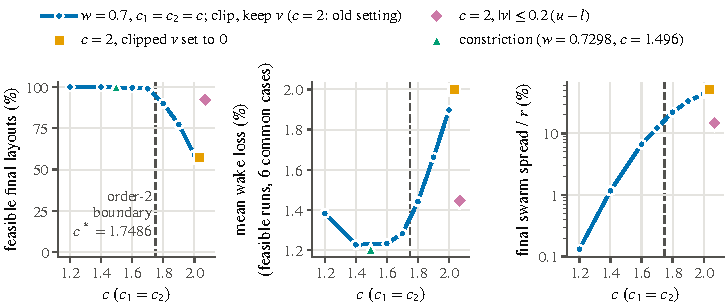
\includegraphics[width=\textwidth]{figures_mpce/csweep.pdf}
\caption{Stand-alone PSO with $w=0.7$ and $c_1=c_2=c$ on the 12 split cases $\times$ 30 seeds (6{,}030 evaluations, random starts; line with circles), the old setting ($c=2$) with two other bound-handling rules (clipped velocity components set to zero; velocity clamping $|v|\le v_{\max}=0.2\,(u-l)$; drawn slightly to the right of $c=2$), and the constriction setting ($w=0.7298$, $c=1.49618$; stored runs of the main comparison, spread not logged). The dashed vertical line is the order-2 stability boundary $c^\ast=12(1-w^2)/(7-5w)=1.7486$ of Proposition~\ref{prop:S-pso-stability} (stagnation, no bounds). Left: feasible final layouts (\% of 360 runs). Middle: mean wake loss of the feasible runs, averaged over the 6 cases in which every setting has at least 15 feasible runs. Right: median final swarm spread (mean over particles of the RMS turbine distance to the global best), relative to the farm radius (log scale). All settings start from the same seeded initial swarm. Values: Table~\ref{tab:S-csweep}.}
\label{fig:S-csweep}
\end{figure*}
\endgroup
\emph{Coefficient sweep.} A sweep of $c_1=c_2=c$ at $w=0.7$ (Fig.~\ref{fig:S-csweep} and Table~\ref{S-tab:S-csweep}; \NSRuns{} runs per setting; $c=2.0$ reproduces the stored old-setting runs bit for bit) shows that the boundary $c^\ast=\NSBoundC$ marks approximately where this PSO starts to fail: at least \NSFeasBelow\% of the runs are feasible for $c\le\NSCBelow$, then feasibility declines progressively (\NSFeasAbove\% at $c=\NSCAbove$, \NSFeasCTwoZero\% at 2.0); velocity clamping raises it to \NSFeasVMax\%, still worse than constriction in all \NSLossCasesVMaxConstr{} cases.
% CHECK-CSWEEP [S01] c = 2.0 reproduces the stored old-setting runs; [S02] c <= 1.7 >= 98 % feasible; [S03] c = 1.8 > 1.9 > 2.0; [S04] decline starts in the step containing c*; [S05] progressive, no jump; [S10] vmax >= 90 %; [S11] vmax worse than constriction in all 12 cases (never "causes")
There is no step at $c^\ast$: the decline begins between 1.7 and 1.8 and accelerates, while the swarm spread grows smoothly with $c$ (by about an order of magnitude from $c=1.4$ to 1.7) and the wake loss rises already on the stable side (lower at $c=1.6$ than at 1.7 in \NSLossBetterSixSeven{} of \NSLossCasesSixSeven{} cases, $p=\NSLossPSixSeven$), then in all \NSLossCasesSevenEight{} cases from 1.7 to 1.8. The boundary marks where the steps become too large for this bounded problem; the sweep does not show that crossing it causes the failure.
% CHECK-CSWEEP [S06] spread grows monotonically, >= 5x from 1.4 to 1.7; [S07] loss degrades on the stable side, c = 1.6 beats 1.7 in >= 10 of 12 (Wilcoxon p < 0.05); [S08] 1.7 -> 1.8 worsens the loss in all 12 cases
Zeroing clipped velocity components does not rescue the old setting (\NSFeasVZero\% feasible), whereas clamping brings it to about the level of $c=1.8$: the deficit comes mainly from the large steps, not from the bound handling.
% CHECK-CSWEEP [S09] zeroing clipped velocities no rescue; [S12] vmax indistinguishable from c = 1.8

Table~\ref{tab:baseline} shows the effect on a comparison. It ranks an eight-method pool, the methods of Table~\ref{tab:friedman68} with LX-SSA-VNS instead of PSO-VNS, once with each PSO setting (all other methods use identical runs): with the old setting, \NBaseOldBest{} ranks first and PSO only in position \NBaseOldPSOPos{}, behind both salp-swarm hybrids; with the constriction setting, \NBaseNewBest{} ranks first, ahead of every salp-swarm method (standard coefficients~\cite{Clerc2002}; none of the methods was tuned on these cases). The reversal holds at 6,030 evaluations; on the six largest cases at 120,030, SSA-VNS ranks ahead of PSO (\NBudRankSSAVNSOneTwentyK{} vs.\ \NBudRankPSOOneTwentyK; Section~\ref{sec:budget}). The old setting thus makes the methods compared with it, including our own LX-SSA, appear stronger than they are.
% CHECK-FINAL [C27]: same pool: old setting SSA-VNS (1.99) and LX-SSA-VNS (2.65) ahead of PSO (5.04, NBaseOldPSOPos); constriction PSO ahead of every salp-swarm method (NBaseNewBest = PSO)
% CHECK-FINAL [C45]: at 120,030 evaluations SSA-VNS ranks ahead of PSO on the six largest cases

\subsection{Overall Comparison}
\label{sec:overall}
% >>>>> begin analysis/mpce_tab_friedman68.tex
%% generated by mpce_results.py -- do not edit by hand
\begin{table}[!t]
\centering
\caption{Case-Level Analysis of the Eight Methods over the 68 Benchmark Cases}
\label{tab:friedman68}
\scriptsize\setlength{\tabcolsep}{2pt}
\begin{tabular}{lcccccc}
\toprule
Method & Avg.\ rank & Best & Feas. & $p_z$ & $p_W$ & $\overline{\Delta L}$ \\
\midrule
PSO-VNS & 1.82 & 29 & 100.0 & -- & -- & -- \\
PSO & 1.97 & 25 & 100.0 & 0.713 & 0.296 & $-0.018$ \\
SSA-VNS & 3.45 & 0 & 99.6 & $2.0\times10^{-4}$ & $5.7\times10^{-11}$ & $-0.330$ \\
VNS & 4.40 & 3 & 100.0 & $2.4\times10^{-9}$ & $1.3\times10^{-10}$ & $-0.465$ \\
SSA & 5.38 & 0 & 97.6 & $8.3\times10^{-17}$ & $4.5\times10^{-11}$ & $-0.611$ \\
MS-SLSQP & 5.88 & 1 & 100.0 & $1.8\times10^{-21}$ & $4.2\times10^{-11}$ & $-0.435$ \\
LX-SSA & 6.06 & 0 & 96.9 & $3.3\times10^{-23}$ & $4.5\times10^{-11}$ & $-0.765$ \\
DE & 7.04 & 0 & 71.4 & $1.0\times10^{-34}$ & $5.6\times10^{-11}$ & $-0.887$ \\
\bottomrule
\end{tabular}
\par\vspace{2pt}\parbox{\columnwidth}{\scriptsize Avg.\ rank: average rank of the mean feasible objective (1 = best; fewer than 15 feasible runs in a case = ranked last); Best: cases in which the method alone ranks first; Feas.: feasible runs (\%); $p_z$: Holm-adjusted $p$ of the average-rank test against PSO-VNS. Because mean-rank tests depend on the pool~\cite{Benavoli2016}, $p_W$ gives the two-sided Wilcoxon signed-rank test on the 68 per-case mean wake losses (Holm-adjusted over the 7 methods) and $\overline{\Delta L}$ the mean wake-loss difference (pp, PSO-VNS minus method; negative = PSO-VNS better) over the cases in which both methods have at least 15 feasible runs (66 for SSA, 66 for LX-SSA, 50 for DE, otherwise 68). Friedman $\chi^2_F=319.3$ (7 d.f.), $p=4.6\times10^{-65}$; Iman--Davenport $F_F=136.5$ (7, 469 d.f.), $p=6.7\times10^{-109}$.}
\end{table}
% <<<<< end analysis/mpce_tab_friedman68.tex
% >>>>> begin analysis/mpce_tab_wtl.tex
%% generated by mpce_results.py -- do not edit by hand
\begin{table}[!t]
\centering
\caption{Run-Level Outcome of PSO-VNS Against Each Method (W/T/L over the 68 Cases)}
\label{tab:wtl}
\scriptsize\setlength{\tabcolsep}{1.6pt}
\begin{tabular}{llcccccccc}
\toprule
DS & $r$ (m) & Cases & PSO & \begin{tabular}{@{}c@{}}SSA-\\VNS\end{tabular} & SSA & \begin{tabular}{@{}c@{}}LX-\\SSA\end{tabular} & DE & VNS & \begin{tabular}{@{}c@{}}MS-\\SLSQP\end{tabular} \\
\midrule
I & 500 & 9 & 0/8/1 & 6/3/0 & 8/1/0 & 8/1/0 & 7/2/0 & 6/3/0 & 7/2/0 \\
I & 750 & 11 & 1/8/2 & 9/2/0 & 10/1/0 & 10/1/0 & 9/2/0 & 8/3/0 & 10/1/0 \\
I & 1000 & 14 & 3/11/0 & 9/5/0 & 12/2/0 & 12/2/0 & 12/2/0 & 12/2/0 & 12/2/0 \\
II & 500 & 9 & 3/5/1 & 7/2/0 & 7/2/0 & 8/1/0 & 7/2/0 & 7/1/1 & 8/1/0 \\
II & 750 & 11 & 2/9/0 & 8/3/0 & 10/1/0 & 10/1/0 & 9/2/0 & 8/3/0 & 9/2/0 \\
II & 1000 & 14 & 5/9/0 & 10/4/0 & 12/2/0 & 12/2/0 & 12/2/0 & 10/4/0 & 13/1/0 \\
\midrule
All & & 68 & 14/50/4 & 49/19/0 & 59/9/0 & 60/8/0 & 56/12/0 & 51/16/1 & 59/9/0 \\
$\tilde r_{\rm rb}$ & & & +0.08 & +0.72 & +0.98 & +0.97 & +1.00 & +0.84 & +0.99 \\
\bottomrule
\end{tabular}
\par\vspace{2pt}\parbox{\columnwidth}{\scriptsize W/T/L: cases in which PSO-VNS is significantly better / not different / worse (two-sided Wilcoxon signed-rank test on 30 seed-paired runs, $\alpha=0.05$, Holm-adjusted over the seven comparisons of PSO-VNS in each case, a different family from Table~\ref{tab:ablation}; an infeasible run ranks below every feasible run). $\tilde r_{\rm rb}$: median rank-biserial correlation (positive = PSO-VNS better; zero differences dropped, $r_{\rm rb}=0$ if all are zero).}
\end{table}
% <<<<< end analysis/mpce_tab_wtl.tex

Over the eight methods (Table~\ref{tab:friedman68}), the Friedman test \NFriedVerb{} the hypothesis of equal performance ($\chi^2_F=\NFriedChi$, $p=\NFriedP$; Iman--Davenport $F_F=\NImanF$, $p=\NImanP$). PSO-VNS has the best average rank (\NRankPSOVNS), alone ranks first in \NSoleBestPSOVNS{} cases, and stays first when the final layouts are re-evaluated with 5$^\circ$ or 1$^\circ$ direction sub-bins (1$^\circ$: \NFRankPSOVNSOne; Section~\ref{sec:robustness}). In the Holm-adjusted post hoc tests ($p_z$ in Table~\ref{tab:friedman68}; tied ranks make them conservative), PSO-VNS ranks significantly better than \NPostHocSigList{}, but not than \NPostHocNonSigList{} ($p_{\rm Holm}=\NPostHocNonSigP$). The rank order and these conclusions are unchanged for thresholds of \NXThrList{} feasible runs; significant comparisons with PSO-VNS favor the same method in each of the \NXClusters{} clusters, and leaving out one cluster changes none of them (Tables~\ref{S-tab:X-threshold}--\ref{S-tab:X-loco}).
% CHECK-FINAL [C01]: main.friedman.best_ranked == PSOBV; [C02]: p < 0.05 (verb generated: \NFriedVerb); [C03]: p_holm_vs_focus: only PSOC >= 0.05
% CHECK-DIR [F06]: PSO-VNS best average rank with 5-deg and 1-deg sub-bins (\NFRankPSOVNSOne)
% CHECK-EXTRA [X02][X03][X05]-[X09] six thresholds 1-30; [X11] clusters 6/6 same direction for comparisons with PSO-VNS; [X14] LOCO changes only \NXLocoChanged (not a PSO-VNS comparison), PSO-VNS always best

% Page budget: the rank chart stays in the supplementary material (Fig. S-fig:S-ranks); the main-text version was:
% \begin{figure}[!t]
% \centering
% \pipefig{0.4\textwidth}{figures_mpce/avg_ranks.pdf}{5cm}
% \caption{Average rank of the eight methods of the main comparison over the 68 benchmark cases (feasibility-aware ranking of Table~\ref{tab:friedman68}; 1 = best).}
% \label{fig:ranks}
% \end{figure}
% CHECK (pipeline): avg_ranks.pdf is drawn from the same ranks as tab:friedman68 (\NRankPSOVNS ... \NRankDE)
In Fig.~\ref{S-fig:S-ranks}, the two PSO-based methods lead with a small gap, far ahead of SSA-VNS; both hybrids rank ahead of their first phase and of VNS, and the last rank of DE also reflects its feasibility (\NFeasDE\% of its runs).
% CHECK (pipeline): rank values from tab:friedman68; [C01] PSO-VNS best; DE feasibility \NFeasDE (CHECK-FINAL [C08])

Against SSA-VNS, PSO-VNS is significantly better in \NWtlSSAVNSW{} cases and never worse ($p_{\rm Holm}=\NPWSSAVNS$). Against SSA, LX-SSA, DE, VNS and MS-SLSQP (untuned DE; finite-difference gradients), it is significantly better in most cases; \NLossesPhrase. PSO-VNS is more reliable in reaching feasibility on the Horns Rev~1 block with random starts (\NHRFeasPSOVNS{} vs.\ \NHRFeasPSO{}, McNemar $p=\NXHRMcNemarP$; Section~\ref{sec:hornsrev-site}) and ranks best on the six largest cases at all three budgets (exploratory; Section~\ref{sec:budget}). The leading methods depend on the conditions: from feasible starts, \NFbFeasBestRank{} ranks first (Section~\ref{sec:feasinit}); under the Gaussian wake, \NBestGauss{} ranks narrowly ahead of PSO-VNS with 15$^\circ$ bins but not with 1$^\circ$ sub-bins (Section~\ref{sec:gaussian}).
% CHECK-FINAL [C06]: wtl.SSABV.L == 0; [C07]: better than SSA, LX-SSA, DE, VNS, MS-SLSQP in most cases; [C08]/[C20]: Horns Rev PSO-VNS 30/30, PSO < 30/30; [C29]: six largest cases best at all budgets; [C28]: feasible-start BVNS best; [C22]: Gauss 15 deg PSOC first, PSOBV second
% CHECK-EXTRA [X52] McNemar (one site, random starts); CHECK-DIR [F06] best rank 15/5/1 deg; [F09] Gaussian: PSO first at 15 deg, PSO-VNS at 1 deg

\begin{figure*}[!t]
\centering
\pipefig{0.72\textwidth}{figures_mpce/wakeloss_vs_n.pdf}{8cm}
\caption{Mean wake loss (\% of the wake-free benchmark objective) of the feasible runs versus the prescribed number of turbines $N$, for each farm and wind data set (30 runs of 6,030 evaluations, random initialization). A point is drawn only when the method has at least 15 feasible runs in that case, so a curve (mostly DE) stops where the method has too few feasible runs.}
\label{fig:wakeloss}
\end{figure*}
The wake loss grows with $N$, falls as the farm becomes larger, and is higher for the broader wind rose of Data Set~II (Fig.~\ref{fig:wakeloss}). PSO-VNS ends feasible in all runs (DE: \NFeasDE\%). In the densest cases (500~m, $N=10$), the global best of the PSO phase is feasible at the switch in only \NDenseSwitchFeas\% of the runs, but all runs are feasible after the VNS phase.
% CHECK-FINAL [C42]: case-mean wake loss grows with N, falls with r, DS II >= DS I; [C08]: feasible_pct.PSOBV == 100; [C24]: dense_500_10 feasible at switch < 100
For the smallest $N$, all methods reach almost no wake loss, so these cases cannot separate the methods; the curves fan out with $N$, most in the small farm and under the broad rose of Data Set~II.
% CHECK-FINAL [C42] (monotone in N, r, data set); curves: wakeloss_vs_n.pdf from the case means of tab:friedman68 runs

\begin{figure*}[!t]
\centering
\pipefig{0.7\textwidth}{figures_mpce/ablation_convergence.pdf}{6.6cm}
\caption{Convergence of the \NAblNVar{} component-analysis variants (Table~\ref{tab:ablation}) for the largest turbine count of each farm: median best feasible wake loss over 30 runs versus evaluations. PSO-VNS and PSO coincide up to 3,030 evaluations (dotted line), where PSO-VNS switches to VNS. Curves of the main comparison: Fig.~\ref{S-fig:S-conv-max} of the supplementary material.}
\label{fig:conv-max}
\label{fig:ablation}
\end{figure*}
% CHECK (pipeline count): \NAblNVar = variants of tab:ablation = curves of ablation_convergence.pdf; [C58] ranks

After the switch, both keep improving (Fig.~\ref{fig:conv-max}): the VNS phase removes on average \NPhTwoMean\% (median \NPhTwoMedian\%) of the wake loss left after the PSO phase and repairs \NPhTwoMadeFeas{} runs infeasible at the switch, whereas continuing PSO for the same 3,000 evaluations removes \NPsoContMean\% (median \NPsoContMedian\%).
% CHECK-FINAL [C10]: phase2 PSOBV.mean >= PSOC_continued.mean > 0 ("both keep improving")

\subsection{PSO-VNS versus PSO}
\label{sec:psovns-pso}
Against PSO, PSO-VNS is significantly better in \NWtlPSOW{} cases, tied in \NWtlPSOT{} and worse in \NWtlPSOL{} (run level, Table~\ref{tab:wtl}). The case means do not differ significantly ($\overline{\Delta L}=\NCmPSOVNSvsPSODL$~pp, $p=\NCmPSOVNSvsPSOP$; Hodges--Lehmann estimate \NXHLPSOVNSvsPSO~pp). Whether the difference is negligible at the post hoc margin $\pm\NEqMargin$~pp depends on the level of inference (Table~\ref{tab:X-equiv-levels}): on this fixed benchmark (seed level), PSO-VNS has a small significant advantage inside the margin (90\% CI \NXEqSeedPSOVNSvsPSOCI); over exchangeable cases the two are equivalent (\NXEqCasePSOVNSvsPSOCI, TOST $p=\NXEqCasePSOVNSvsPSOP$, minimal margin \NXEqCasePSOVNSvsPSOMin); over farm clusters, equivalence is not shown (CR2 \NXEqClustPSOVNSvsPSOCI, minimal margin \NXEqClustPSOVNSvsPSOMin). In the Bayesian signed-rank test, practical equivalence is the most probable outcome (posterior probability \NBayPSOVNSvsPSORope; posterior means \NXBayMeanPSOVNSvsPSOLeft/\NXBayMeanPSOVNSvsPSORope/\NXBayMeanPSOVNSvsPSORight{} for PSO-VNS better by more than the margin/equivalent/PSO better). The margin corresponds to \NXMarginMWhTurbDsI{} (Data Set~I) and \NXMarginMWhTurbDsII~MWh/yr (Data Set~II) per turbine, the mean gain of PSO-VNS to \NXEnPSOVNSvsPSOMWhTurb~MWh/yr per turbine (\NXEnPSOVNSvsPSOPct\% of AEP). Spread and worst run do not differ ($p=\NSdP$, \NWorstP).
% CHECK-FINAL [C04]: PSOC: W >= L, mean loss PSOBV < PSOC, case-mean p >= 0.05; [C49]: case-level 90% CI inside +-m, P(rope most probable) printed via \NBayPSOVNSvsPSORope; [C52]: SD p and worst-run p >= 0.05
% CHECK-EXTRA [X39] seed and case level equivalent, cluster level not; [X40] seed-level CI excludes 0 inside m; [X41] minimal margins seed < case < m < cluster; [X48] Bayesian wording + posterior means; [X50] HL near 0; [X56] margin 4.1/2.1 MWh/yr per turbine, mean gain 0.2; [X25] energy < 0.05 % AEP

\begingroup\swResRefs
%
% --- float tab:X-equiv-levels from analysis/mpce_supp_inference.tex
\begin{table}[!htbp]
\centering
\caption{Practical equivalence (margin $m=0.05$~pp, set after the primary analysis) of the pairs of Table~\ref{tab:equivalence} at three levels of inference. $\overline{\Delta L}$: mean over the $n$ cases of the case-mean wake-loss difference, first minus second method (pp; negative = first better; the same estimate at every level). \emph{Seed level} (fixed benchmark: the 68 cases are fixed and only the run-to-run variability is random): 10{,}000 bootstrap resamples of the 30 seed-paired runs within every case (same seeds for both methods; case means over the feasible resampled runs), percentile 90\% CI. \emph{Case level} (generalization to exchangeable cases, as Table~\ref{tab:equivalence}): percentile bootstrap over the cases; $p_{\rm TOST}$ as there. \emph{Cluster level} (generalization to new farms; 6 (data set, radius) clusters): cluster-robust 90\% CI with the CR2 (bias-reduced) variance and a $t$ distribution with 5 d.f. (Bell--McCaffrey d.f.\ 4.8 for PSO-VNS vs.\ PSO), and a restricted wild-cluster bootstrap-$t$ TOST (CR2-studentized, all 46{,}656 draws of the Webb six-point weights enumerated; $m_{\min}$ by test inversion). $m_{\min}$: smallest margin at which equivalence holds (rounded up). Eq.: equivalent at $\pm m$ (cluster level: CR2 CI inside $\pm m$ and wild $p_{\rm TOST}\le0.05$).}
\label{tab:X-equiv-levels}
\scriptsize\setlength{\tabcolsep}{2pt}
\resizebox{\textwidth}{!}{%
\begin{tabular}{lcccccccccccccc}
\toprule
& & & \multicolumn{3}{c}{Seed level} & \multicolumn{4}{c}{Case level} & \multicolumn{5}{c}{Cluster level} \\
\cmidrule(lr){4-6}\cmidrule(lr){7-10}\cmidrule(lr){11-15}
Pair (first vs.\ second) & $n$ & $\overline{\Delta L}$ & 90\% CI & $m_{\min}$ & Eq. & 90\% CI & $m_{\min}$ & $p_{\rm TOST}$ & Eq. & CR2 90\% CI & $m_{\min}$ & wild $p_{\rm TOST}$ & wild $m_{\min}$ & Eq. \\
\midrule
\multicolumn{15}{l}{\emph{Component-analysis contrasts}} \\
SSA-VNS vs.\ RS-VNS & 68 & $-0.068$ & [$-$0.092, $-$0.044] & 0.093 & no & [$-$0.101, $-$0.039] & 0.102 & 0.839 & no & [$-$0.126, $-$0.011] & 0.126 & 0.716 & 0.130 & no \\
LX-SSA-VNS vs.\ RS-VNS & 68 & $-0.005$ & [$-$0.030, 0.020] & 0.031 & yes & [$-$0.034, 0.021] & 0.035 & 0.008 & yes & [$-$0.061, 0.051] & 0.062 & 0.082 & 0.068 & no \\
PSO-VNS vs.\ RS-VNS & 68 & $-0.399$ & [$-$0.420, $-$0.378] & 0.421 & no & [$-$0.479, $-$0.324] & 0.479 & 1.000 & no & [$-$0.544, $-$0.254] & 0.544 & 0.995 & 0.557 & no \\
SSA-VNS vs.\ LX-SSA-VNS & 68 & $-0.063$ & [$-$0.086, $-$0.040] & 0.086 & no & [$-$0.086, $-$0.042] & 0.087 & 0.841 & no & [$-$0.087, $-$0.039] & 0.088 & 0.843 & 0.087 & no \\
LX-SSA vs.\ SSA & 66 & $+0.153$ & [0.123, 0.185] & 0.185 & no & [0.104, 0.206] & 0.207 & 1.000 & no & [0.109, 0.198] & 0.198 & 0.995 & 0.213 & no \\
SSA-VNS vs.\ SSA & 66 & $-0.294$ & [$-$0.319, $-$0.269] & 0.319 & no & [$-$0.368, $-$0.226] & 0.368 & 1.000 & no & [$-$0.371, $-$0.216] & 0.372 & 0.995 & 0.376 & no \\
LX-SSA-VNS vs.\ LX-SSA & 66 & $-0.394$ & [$-$0.422, $-$0.367] & 0.423 & no & [$-$0.505, $-$0.293] & 0.506 & 1.000 & no & [$-$0.467, $-$0.321] & 0.468 & 0.997 & 0.467 & no \\
PSO-VNS vs.\ PSO & 68 & $-0.018$ & [$-$0.026, $-$0.010] & 0.026 & yes & [$-$0.041, 0.004] & 0.041 & 0.011 & yes & [$-$0.067, 0.031] & 0.067 & 0.105 & 0.067 & no \\
PSO-VNS vs.\ VNS & 68 & $-0.465$ & [$-$0.489, $-$0.442] & 0.489 & no & [$-$0.545, $-$0.386] & 0.546 & 1.000 & no & [$-$0.593, $-$0.338] & 0.593 & 0.996 & 0.575 & no \\
SSA-VNS vs.\ RSD-VNS & 68 & $+0.024$ & [0.002, 0.046] & 0.047 & yes & [$-$0.022, 0.062] & 0.062 & 0.141 & no & [$-$0.051, 0.099] & 0.100 & 0.263 & 0.089 & no \\
LX-SSA-VNS vs.\ RSD-VNS & 68 & $+0.087$ & [0.065, 0.110] & 0.111 & no & [0.047, 0.126] & 0.126 & 0.936 & no & [0.004, 0.170] & 0.171 & 0.788 & 0.165 & no \\
PSO-VNS vs.\ RSD-VNS & 68 & $-0.306$ & [$-$0.325, $-$0.287] & 0.326 & no & [$-$0.380, $-$0.239] & 0.381 & 1.000 & no & [$-$0.442, $-$0.171] & 0.442 & 0.994 & 0.454 & no \\
RSD-VNS vs.\ RS-VNS & 68 & $-0.093$ & [$-$0.115, $-$0.070] & 0.115 & no & [$-$0.127, $-$0.055] & 0.128 & 0.971 & no & [$-$0.131, $-$0.054] & 0.131 & 0.967 & 0.132 & no \\
\midrule
\multicolumn{15}{l}{\emph{Main comparison, PSO-VNS vs.\ each method (PSO and VNS: see above)}} \\
PSO-VNS vs.\ SSA-VNS & 68 & $-0.330$ & [$-$0.350, $-$0.310] & 0.351 & no & [$-$0.397, $-$0.266] & 0.397 & 1.000 & no & [$-$0.434, $-$0.227] & 0.434 & 0.997 & 0.430 & no \\
PSO-VNS vs.\ SSA & 66 & $-0.611$ & [$-$0.633, $-$0.589] & 0.633 & no & [$-$0.735, $-$0.493] & 0.735 & 1.000 & no & [$-$0.770, $-$0.452] & 0.771 & 0.996 & 0.753 & no \\
PSO-VNS vs.\ LX-SSA & 66 & $-0.765$ & [$-$0.791, $-$0.739] & 0.792 & no & [$-$0.930, $-$0.606] & 0.930 & 1.000 & no & [$-$0.946, $-$0.583] & 0.946 & 0.997 & 0.921 & no \\
PSO-VNS vs.\ DE & 50 & $-0.887$ & [$-$0.916, $-$0.858] & 0.917 & no & [$-$1.137, $-$0.648] & 1.137 & 1.000 & no & [$-$1.173, $-$0.600] & 1.174 & 0.994 & 1.169 & no \\
PSO-VNS vs.\ MS-SLSQP & 68 & $-0.435$ & [$-$0.452, $-$0.419] & 0.452 & no & [$-$0.505, $-$0.366] & 0.505 & 1.000 & no & [$-$0.579, $-$0.291] & 0.580 & 0.994 & 0.580 & no \\
\bottomrule
\end{tabular}}
\end{table}

\begin{figure}[!t]
\centering
\pipefig{0.45\textwidth}{figures_mpce/equiv_curve.pdf}{5cm}
\caption{Equivalence curve of PSO-VNS vs.\ PSO: TOST $p$ value versus the equivalence margin $m$ (pp of wake loss) at three levels of inference (Table~\ref{tab:X-equiv-levels}): seed level (fixed benchmark; bootstrap of the seed-paired runs within every case), case level (bootstrap over the 68 cases, as Table~\ref{tab:equivalence}) and cluster level (six farm clusters; CR2 cluster-robust $t$ with 5 d.f., and the restricted wild-cluster bootstrap). Dotted lines: $\alpha=0.05$ and the margin $m=\NEqMargin$~pp. The dots mark the minimal margins $m_{\min}$, at which a curve crosses $\alpha$; equivalence holds at every margin to the right of the dot. The bootstrap curves stop at their resolution limit $1/10{,}001$.}
\label{fig:equiv-curve}
\end{figure}
\endgroup
% CHECK-EXTRA [X57] equiv_curve.pdf generated in the same run; [X41] minimal margins seed < case < m < cluster
The levels ask whether new seeds on this fixed benchmark would reproduce the difference (seed), whether it holds for exchangeable cases like these (case), and whether it carries over to new farms, given six clusters with nested $N$ (cluster; five d.f.). The minimal margin grows with the scope; as the post hoc margin lies just above the case-level value, Fig.~\ref{fig:equiv-curve} gives the whole TOST curve. The seed-level interval excludes zero: the methods differ reproducibly here, but by less than the margin. No pair is equivalent at the cluster level.
% CHECK-EXTRA [X39]-[X41]; [X55] no pair equivalent at the cluster level; main-comparison pairs other than PSO: whole 90% CI beyond -m at all three levels (tab:X-equiv-levels, m_min > m)

\begingroup\swResRefs\swResWrapNotes
% Page budget: kept in the supplementary material: \SuppTable{tab:X-heterogeneity}
\endgroup
The average hides case-level differences in both directions: \NXHetBeyondPSOVNS{} cases favor PSO-VNS by more than the margin (by up to \NXHetMaxPSOVNS~pp) and \NXHetBeyondPSO{} favor PSO (up to \NXHetMaxPSO~pp; Table~\ref{S-tab:X-heterogeneity}). The two are equivalent for $N<10$ (\NXEqSmallN{} cases, 90\% CI \NXEqSmallCI) but not for $N\ge10$ (\NXEqLargeMean~pp, \NXEqLargeCI) or on the \NXEqNontrivialN{} cases with a wake loss of at least \NXTrivialLoss~pp (\NXEqNontrivialCI). They follow a data set $\times$ density crossover (density $\phi=\NXDensDef$; stated after review, exploratory; interaction $p=\NXDensInterP$): as $\phi$ grows, PSO-VNS gains in Data Set~II (slope \NXDensSlopeDsII~pp, $p=\NXDensPDsII$) and PSO in Data Set~I (\NXDensSlopeDsI~pp, $p=\NXDensPDsI$). In the post hoc subgroup Data Set~II, $N\ge10$, PSO-VNS has the lower mean wake loss in \NCmPSOVNSvsPSOdsIILargeWins{} of \NCmPSOVNSvsPSOdsIILargeN{} cases ($p_{\rm Holm}\le\NXHolmPSOVNSvsPSOdsIILargeP$ over all \NXMultN{} case-mean Wilcoxon tests; \NXEnPSOVNSvsPSOdsIILargePct\% of AEP); all \NXHetDsINPSO{} Data Set~I cases beyond the margin favor PSO. With 1$^\circ$ sub-bins, PSO-VNS is slightly but significantly better than PSO ($\overline{\Delta L}=\NFPairMeanOne$~pp, 90\% CI \NFPairCIOne; Table~\ref{S-tab:F-equiv}).
% CHECK-EXTRA [X43] 11/8 beyond +-m, max 0.41/0.27; [X44] N < 10 equivalent, N >= 10 not; [X45] non-trivial cases not equivalent; [X47] data set x density crossover (exploratory, stated after review); [X19] DS II N >= 10 survives all-family Holm ("<=", R5 O13); [X27] DS II N >= 10 ~0.2 % AEP
% CHECK-FINAL [C32]: DS II N >= 10 case-mean wins > losses
% CHECK-DIR [F10]: 1-deg PSO-VNS - PSO CI below 0, not equivalent; [F14]: DS II N >= 10 advantage survives at 1 deg

The average verdict thus depends on the case mix: in the \NXEqTrivialN{} cases with a PSO-VNS wake loss below \NXTrivialLoss~pp, both find almost wake-free layouts and none differs by more than the margin. The differences are structured (\NXHetClBeyond{} of \NXClustersNum{} cluster means beyond the margin, in both directions): in Data Set~II, \NXHetDsIINPSOVNS{} cases beyond the margin, the larger layouts of all three farms, favor PSO-VNS, and in Data Set~I all \NXHetDsINPSO{}, dense layouts in the two smaller farms, favor PSO (Table~\ref{S-tab:X-beyond}). The crossover, found after review with no cause identified, is a hypothesis for designed experiments. PSO-VNS thus does not dominate a well-configured PSO: it is at least as good on average, gains in larger Data Set~II layouts and loses in dense Data Set~I layouts.
% CHECK-EXTRA [X44] N < 10 (48 cases) equivalent; [X45] trivial cases equivalent, every case beyond the margin non-trivial, non-trivial not equivalent; [X46] 3 of 6 cluster means beyond +-m in opposite directions (2 PSO-VNS, 1 PSO; DS I 500 m, DS II 1000 m); [X47] DS I cases beyond the margin all favor PSO and are dense, DS II 11 favor PSO-VNS, 1 favors PSO (exploratory, stated after review)
% <<<<< end optA/sw/06_results.tex
% >>>>> begin optA/sw/07_ablation.tex
\section{Component Analysis of Two-Phase Hybrids}
\label{sec:ablation}
% SWEVO extension: the generated tables tab:D-vns and tab:D-rsreplay are captured from analysis/mpce_supp_diag.tex (its
% figure fig:D-psodyn is discarded here, not placed); tab:switch and tab:equivalence come from the global capture of
% analysis/mpce_supplementary.tex, tab:split from analysis/mpce_tab_split.tex (all logged in optA/sw/moved.md)
\begingroup\RenewEnviron{figure*}[1][]{}\endgroup% [flattened: removed \CaptureSuppTables{analysis/mpce_supp_diag.tex}]
% [flattened: removed \CaptureSuppTables{analysis/mpce_tab_split.tex}]
\makeatletter
% \AblTable[<placement>]{<label>}: like \SuppTable (placed once, TBD box if absent), with a placement of our choice
\newcommand{\AblTable}[2][!t]{\@ifundefined{supp@body@#2}{\SuppTable{#2}}{\@ifundefined{supp@used@#2}{%
  \global\@namedef{supp@used@#2}{}\begin{table}[#1]\@nameuse{supp@body@#2}\end{table}}{}}}
% posterior probabilities in math mode: "= value", or "< 0.01" / "> 0.99" for a bound (rule of \BayEq in the supplement)
\newcommand{\AblBayEq}[1]{\expandafter\abl@bayeq#1\@nil}
\def\abl@bayeq#1#2\@nil{\ifx#1\ensuremath #2\else =#1#2\fi}
\makeatother
% >>>>> begin analysis/mpce_tab_ablation.tex
%% generated by mpce_results.py -- do not edit by hand
\begin{table}[!t]
\centering
\caption{Component Analysis over the 68 Benchmark Cases (6,030 Evaluations, 30 Seed-Paired Runs)}
\label{tab:ablation}
\scriptsize\setlength{\tabcolsep}{2.5pt}
\begin{tabular}{lcccc}
\toprule
Variant & Phase 1 & Phase 2 & Avg.\ rank & Feas.\ (\%) \\
\midrule
PSO-VNS & PSO & VNS & 1.96 & 100.0 \\
SSA-VNS & SSA & VNS & 4.46 & 99.6 \\
LX-SSA-VNS & LX-SSA & VNS & 5.41 & 99.9 \\
RS-VNS & random (square) & VNS & 5.29 & 99.4 \\
RSD-VNS & random (disc) & VNS & 3.77 & 99.8 \\
VNS & -- & VNS & 6.12 & 100.0 \\
PSO & PSO & -- & 2.24 & 100.0 \\
SSA & SSA & -- & 7.50 & 97.6 \\
LX-SSA & LX-SSA & -- & 8.25 & 96.9 \\
\bottomrule
\end{tabular}

\smallskip
\begin{tabular}{l>{\raggedright\arraybackslash}p{1.95cm}ccc}
\toprule
Contrast & Isolates & W/T/L & $p_W$ & $\overline{\Delta L}$ \\
\midrule
PSO-VNS vs.\ PSO & VNS phase (PSO) & 8/58/2 & 0.592 & $-0.018$ \\
SSA-VNS vs.\ SSA & VNS phase (SSA) & 39/29/0 & $5.7\times10^{-10}$ & $-0.294$ \\
LX-SSA-VNS vs.\ LX-SSA & VNS phase (LX-SSA) & 34/34/0 & $1.1\times10^{-10}$ & $-0.394$ \\
PSO-VNS vs.\ VNS & swarm start vs.\ best initial point & 49/18/1 & $5.7\times10^{-10}$ & $-0.465$ \\
PSO-VNS vs.\ RS-VNS & PSO vs.\ random sampling & 47/21/0 & $3.2\times10^{-10}$ & $-0.399$ \\
SSA-VNS vs.\ RS-VNS & SSA vs.\ random sampling & 2/66/0 & 0.002 & $-0.068$ \\
LX-SSA-VNS vs.\ RS-VNS & LX-SSA vs.\ random sampling & 1/67/0 & 0.718 & $-0.005$ \\
PSO-VNS vs.\ RSD-VNS & PSO vs.\ disc sampling & 45/23/0 & $4.0\times10^{-10}$ & $-0.306$ \\
SSA-VNS vs.\ RSD-VNS & SSA vs.\ disc sampling & 0/66/2 & 0.014 & $+0.024$ \\
LX-SSA-VNS vs.\ RSD-VNS & LX-SSA vs.\ disc sampling & 1/62/5 & $8.2\times10^{-6}$ & $+0.087$ \\
RSD-VNS vs.\ RS-VNS & disc vs.\ square sampling & 6/62/0 & $4.2\times10^{-7}$ & $-0.093$ \\
PSO-VNS vs.\ SSA-VNS & PSO vs.\ SSA as Phase~1 & 44/24/0 & $2.5\times10^{-10}$ & $-0.330$ \\
PSO-VNS vs.\ LX-SSA-VNS & PSO vs.\ LX-SSA as Phase~1 & 47/21/0 & $2.3\times10^{-10}$ & $-0.393$ \\
SSA-VNS vs.\ LX-SSA-VNS & LX-SSA as published (hybrid) & 2/66/0 & $2.7\times10^{-5}$ & $-0.063$ \\
LX-SSA vs.\ SSA & LX-SSA as published (alone) & 0/64/4 & $1.3\times10^{-6}$ & $+0.153$ \\
\bottomrule
\end{tabular}
\par\vspace{2pt}\parbox{\columnwidth}{\scriptsize Top: average rank among the nine variants (Friedman $\chi^2_F=374.3$, 8 d.f., $p=5.96\times10^{-76}$) and feasible runs. Bottom: planned contrasts. W/T/L: cases in which the first variant is significantly better / not different / worse (run-level Wilcoxon, $\alpha=0.05$, Holm-adjusted over the fifteen contrasts of each case, a different family from Table~\ref{tab:wtl}); $p_W$: Wilcoxon test on the 68 per-case mean wake losses, Holm-adjusted over the fifteen contrasts; $\overline{\Delta L}$: mean difference of the case-mean wake losses (pp; negative = first variant better) over the cases in which both variants have at least 15 feasible runs (66--68 of 68 per contrast).}
\end{table}
% <<<<< end analysis/mpce_tab_ablation.tex

The variants of Table~\ref{tab:ablation} combine a Phase~1 (PSO, SSA, LX-SSA, random sampling or none) with or without the same VNS phase (6,030 evaluations from random starts, same seeds; convergence: Fig.~\ref{fig:ablation}); their average ranks differ (Friedman $p=\NAblP$). W/T/L, $p$ (Holm-adjusted Wilcoxon test on the 68 case means) and $\overline{\Delta L}$ (mean difference of the case means, pp) are those of Table~\ref{tab:ablation}; a 90\% bootstrap interval of $\overline{\Delta L}$ (in brackets) inside $\pm\NEqMargin$~pp means practical equivalence at the case level.
% CHECK-FINAL [C36]: Friedman rejects equal average ranks (\NAblP); pipeline-generated counts \NAblNContrasts (Holm family of each case), \NAblDf d.f., \NAblNVar variants in the caption. All DL in this section are \NCm...DL = tab:ablation values (R1-7, R5-F1)


\subsection{The VNS Phase}
\label{sec:abl-vns}
The VNS phase improves both salp-swarm methods: SSA-VNS is \NAblSSAVNSvsSSA{} (W/T/L) against SSA and LX-SSA-VNS \NAblLXSSAVNSvsLXSSA{} against LX-SSA ($\overline{\Delta L}=\NCmSSAVNSvsSSADL$ and \NCmLXSSAVNSvsLXSSADL). For PSO, which PSO-VNS repeats for its first 3,030 evaluations (Section~\ref{sec:hybrid}), the difference is small, not significant and practically equivalent to zero ($\overline{\Delta L}=\NCmPSOVNSvsPSODL$ \NEqPSOVNSvsPSOCI, $p=\NCmPSOVNSvsPSOPHolm$). At this budget the VNS phase is essentially one compass-search descent: for PSO-VNS, the shake-and-search cycles take \NDCycleEvalsPctPSOVNS\% of the Phase-2 evaluations (pooled; median run \NDCycleEvalsPctMedianPSOVNS\%) but give \NDCycleSharePSOVNS\% of the Phase-2 gain (\NDCycleAllSharePSOVNS\% with the cycle cut off by the budget), and the median run with $N\ge12$ never shakes (Table~\ref{S-tab:D-vns}). The analysis thus measures the value of a local-search phase.
% CHECK-FINAL [C33]: VNS phase significant for SSA and LX-SSA (W > L, L = 0; case-mean p < 0.05, DL < 0), not for PSO (case-mean p >= 0.05, so also Holm); [C13]: PSOBV-PSOC W > L; [C49]: case-level 90 % CI \NEqPSOVNSvsPSOCI inside +-\NEqMargin
% CHECK-DIAG [D20]: cycles >= 15 % of the Phase-2 evaluations, < 5 % of the gain incl. the cut-off cycle, accepted cycles < 1 % (\NDCycleEvalsPctPSOVNS, median run \NDCycleEvalsPctMedianPSOVNS, \NDCycleSharePSOVNS, \NDCycleAllSharePSOVNS); [D08]: essentially one descent; [D09]: median run has no shaking step for N >= 12

% Page budget: kept in the supplementary material: \AblTable{tab:D-vns}
In Table~\ref{S-tab:D-vns} (\NDVnsCases{} split cases $\times$ \NDVnsSeeds{} seeds), the first descent from the switch point takes a median of \NDDescentEvalsPSOVNS{} evaluations in PSO-VNS and gives \NDDescentSharePSOVNS\% of the Phase-2 improvement (SSA-VNS \NDDescentShareSSAVNS\%, RS-VNS \NDDescentShareRSVNS\%). A shake costs one evaluation, but the new descent after it scans $2n=4N$ moves per step, and \NDNoAcceptedPSOVNS{} of \NDVnsRunsPSOVNS{} runs accept no cycle; accepted cycles use only $k=1$. For $N\ge12$ the first descent is unfinished in \NDDescentUnfinishedLargePSOVNS{} of \NDRunsLargePSOVNS{} runs, so the local-minimality guarantee (Proposition~\ref{S-prop:S-ls}) does not apply there. VNS never makes a feasible incumbent infeasible and starts from the best feasible Phase-1 layout when one exists. The contrasts thus test a truncated compass search after Phase~1; shaking and neighborhood change can matter only for small $N$.
% CHECK-DIAG [D08]: median shaking steps <= 2, >= 85 % of the Phase-2 improvement from the first descent for PSO-VNS, SSA-VNS, RS-VNS (\NDDescentSharePSOVNS, \NDDescentShareSSAVNS, \NDDescentShareRSVNS); no accepted cycle in \NDNoAcceptedPSOVNS of 120 runs; [D10]: accepted cycles only with k = 1; [D09]: N >= 12 first descent unfinished (\NDDescentUnfinishedLargePSOVNS of \NDRunsLargePSOVNS); [D11]: VNS never turns a feasible incumbent infeasible; [D12]: start = best feasible Phase-1 layout whenever Phase 1 evaluated one; [D20]: cycles costly relative to their gain

\subsection{Random-Sampling Controls}
\label{sec:abl-controls}
Random sampling of equal cost replaces Phase~1, uniform in the site disc (RSD-VNS) or in its bounding square (RS-VNS); VNS alone is a third control. RS-VNS is weak: \NRSRunsNoFeasSample{} of its runs draw no feasible sample, although all of them draw samples wholly inside the circle: the spacing constraint is binding, and disc sampling rescues only \NRsSquareExplains{} of these runs. RSD-VNS beats RS-VNS (\NAblRSDVNSvsRSVNS, $\overline{\Delta L}=\NCmRSDVNSvsRSVNSDL$) and ranks third (\NRankRSDVNS).
% CHECK-FINAL [C60]: RS-VNS runs without a feasible sample (\NRSRunsNoFeasSample) = rescued by disc sampling (\NRsSquareExplains) + none either way (\NRsSpacingDominates), rescued < none; LEAD: extend C60 with runs_no_feasible_but_inside_sample == runs_no_feasible_sample (\NRsNoFeasInside = \NRSRunsNoFeasSample, mpce_results.py phase1_replay.RSVNS) for "all of them"
% CHECK-FINAL [C57]: RSDVNS-RSVNS L == 0, W > 0, case-mean p_Holm < 0.05, DL < 0; [C58]: RSD-VNS ranks third of \NAblNVar

% Page budget: kept in the supplementary material: \AblTable{tab:D-rsreplay}
Table~\ref{S-tab:D-rsreplay} replays Phase~1 of RS-VNS from the seeded random streams. The share of square samples wholly inside the circle matches $(\pi/4)^N$ (Proposition~\ref{prop:S-box}), but the feasible share vanishes much sooner, as random positions rarely keep all $N(N-1)/2$ pairs $\ell_{\min}$ apart: for $N=15$ in the 1000-m farm, \NDRsInsideNFifteen\% of the \NDRsSamples{} samples lie inside and none is feasible. The \NRSRunsNoFeasSample{} runs without a feasible sample (all runs of \NDRsCasesNoFeasSample{} cases) start VNS from the least-penalized sample; paired by seed, \NRsSquareExplains{} of them would get a feasible sample in the disc and \NRsSpacingDominates{} none. RS-VNS is thus weak mainly because of the spacing, only in part because of the square, and beating it is only a minimum bar.
% CHECK-DIAG [D17]: replay agrees with the runs; inside rate matches (pi/4)^N; N = 15, 1000 m: \NDRsFeasNFifteen of \NDRsSamples box samples feasible; \NDRsRunsNoFeasSample runs (all runs of \NDRsCasesNoFeasSample cases) without a feasible sample; CHECK-FINAL [C60]: rescued \NRsSquareExplains < none either way \NRsSpacingDominates ("mainly because of the spacing")

% Page budget: kept in the supplementary material: \AblTable{tab:switch}
In the disc, the feasible Phase-1 samples rise from \NRSPctFeasSamples\% to \NRSDPctFeasSamples\% and the runs without one fall from \NRSRunsNoFeasSample{} to \NRSDRunsNoFeasSample. At the switch (Table~\ref{S-tab:switch}; controls read at 3,000 evaluations), the best layout is feasible in \NSwitchFeasRSDVNS\% (RSD-VNS) and \NSwitchFeasRSVNS\% (RS-VNS) of the runs, well below the swarm phases, so VNS must often repair the start; the switch loss covers the feasible runs only.
% CHECK-FINAL [C57]: RSD-VNS feasible at the switch more often, fewer runs without a feasible sample (replay verified); [C61]: controls switch at 3,015, read at the checkpoint 3,000; CHECK-DIAG [D18]: feasible by the switch PSO > SSA > RS (RSD-VNS \NSwitchFeasRSDVNS < SSA-VNS \NSwitchFeasSSAVNS: tab:switch values); [D11]: infeasible switch points repaired by the first descent

\subsection{Swarm First Phases}
\label{sec:abl-swarm}
A PSO phase clearly beats every control: PSO-VNS is \NAblPSOVNSvsRSDVNS{} against RSD-VNS ($\overline{\Delta L}=\NCmPSOVNSvsRSDVNSDL$ \NEqPSOVNSvsRSDVNSCI, wholly below $-\NEqMargin$), \NAblPSOVNSvsRSVNS{} against RS-VNS and \NAblPSOVNSvsVNS{} against VNS. At this budget and from random starts, salp-swarm phases add nothing beyond random sampling in the farm. Against RSD-VNS, SSA-VNS is \NAblSSAVNSvsRSDVNS{} ($\overline{\Delta L}=\NCmSSAVNSvsRSDVNSDL$; Hodges--Lehmann estimate \NXHLSSAVNSvsRSDVNS~pp, 95\% CI \NXHLSSAVNSvsRSDVNSCI; the case means, not the farm clusters, favor RSD-VNS): a gain of the SSA phase larger than the margin is ruled out at the seed and the case level (90\% intervals \NXEqSeedSSAVNSvsRSDVNSCI{} and \NXEqCaseSSAVNSvsRSDVNSCI, both above $-\NEqMargin$), whereas equivalence remains inconclusive. LX-SSA-VNS is \NAblLXSSAVNSvsRSDVNS{} and worse ($\overline{\Delta L}=\NCmLXSSAVNSvsRSDVNSDL$, $p=\NCmLXSSAVNSvsRSDVNSPHolm$). The small SSA gain over RS-VNS (\NAblSSAVNSvsRSVNS, $\overline{\Delta L}=\NCmSSAVNSvsRSVNSDL$) only reflects that control's weakness; LX-SSA-VNS and RS-VNS are practically equivalent (\NEqLXSSAVNSvsRSVNSCI). Re-evaluated with 1$^\circ$ direction bins (Table~\ref{S-tab:F-abl}), SSA-VNS and LX-SSA-VNS again have a higher loss than RSD-VNS (\NFAblSSAVNSvsRSDVNSOne{} and \NFAblLXSSAVNSvsRSDVNSOne~pp) and PSO-VNS beats all three controls; only the SSA gain over RS-VNS is no longer significant.
% CHECK-FINAL [C56]: PSOBV-RSDVNS W >= 40, L == 0, p_Holm < 0.05, whole 90 % CI below -\NEqMargin; [C14]: PSOBV-RSVNS L == 0, PSOBV-BVNS L <= 2 ("clearly beats every control")
% CHECK-FINAL [C53]: SSABV-RSDVNS W == 0, case-mean losses > wins, p_Holm < 0.05 against SSA-VNS; CHECK-EXTRA [X33]: not at cluster level ("not the farm clusters"; never "worse"); [X49]: HL > 0, 95 % CI \NXHLSSAVNSvsRSDVNSCI; [X53]: lower 90 % limits above -m at seed and case level, not at cluster level ("ruled out at the seed and the case level"); CHECK-FINAL [C54]: 90 % case CI not inside +-m (equivalence not shown); CHECK-EXTRA [X54]: seed level equivalent, case/cluster not ("inconclusive")
% CHECK-FINAL [C55]: LXBV-RSDVNS L > W, p_Holm < 0.05, DL > 0; CHECK-EXTRA [X34]: CR p 0.087 ("worse", not "clearly worse"); CHECK-FINAL [C15]/[C51]: SSABV-RSVNS small gain, not equivalent; [C50]: LX-SSA-VNS vs RS-VNS equivalent (\NEqLXSSAVNSvsRSVNSCI)
% CHECK-DIR [F16]: 1-deg: SSABV and LXBV higher case-mean loss than RSDVNS (p < 0.05), PSOBV better than RSDVNS, RSVNS, BVNS (p < 0.05); [F17]: 1-deg SSABV-RSVNS p >= 0.05 (\NFAblSSAVNSvsRSVNSOneP)

\emph{LX-SSA as published.} LX-SSA costs $2N_p$ evaluations per iteration (Section~\ref{sec:ssa}) and so runs half as many iterations as SSA; the contrasts do not separate its Laplace step from this cost. As published, it makes the salp swarm worse: LX-SSA is \NAblLXSSAvsSSA{} against SSA ($\overline{\Delta L}=\NCmLXSSAvsSSADL$, $p=\NCmLXSSAvsSSAPHolm$) and SSA-VNS is \NAblSSAVNSvsLXSSAVNS{} against LX-SSA-VNS ($\overline{\Delta L}=\NCmSSAVNSvsLXSSAVNSDL$, $p=\NCmSSAVNSvsLXSSAVNSPHolm$).
% CHECK-FINAL [C17]: LX-SSA as published worse (never "Laplace step harmful"): LXSSA-SSA W == 0; SSABV-LXBV L == 0; case means favour SSA and SSA-VNS (p < 0.05, so also Holm)

\emph{Choice of Phase~1.} With the same VNS phase, PSO-VNS is \NAblPSOVNSvsSSAVNS{} against SSA-VNS and \NAblPSOVNSvsLXSSAVNS{} against LX-SSA-VNS. At the switch, its global best is feasible more often (\NSwitchFeasPSOVNS\% of the runs vs.\ \NSwitchFeasSSAVNS\% and \NSwitchFeasLXSSAVNS\%) and, when feasible, has a lower wake loss (\NSwitchLossPSOVNS\% vs.\ \NSwitchLossSSAVNS\% and \NSwitchLossLXSSAVNS\%). Whether PSO helps mainly by faster feasibility or by better exploration remains open (cf.\ the feasible starts in Section~\ref{sec:feasinit}).
% CHECK-FINAL [C16]: PSOBV-SSABV, PSOBV-LXBV: L == 0, W >= 34; switch feasibility higher and switch loss lower for PSOBV

%
% --- float tab:equivalence from analysis/mpce_supplementary.tex
\begin{table}[!t]
\centering
\caption{Practical equivalence of the per-case mean wake losses at 6,030 evaluations. $\overline{\Delta L}$: mean difference of the case-mean wake losses, first minus second method (percentage points, pp; negative = first method better), over the $n$ cases in which both methods have at least 15 feasible runs out of 30 (cases excluded: LX-SSA vs.\ SSA 2; SSA-VNS vs.\ SSA 2; LX-SSA-VNS vs.\ LX-SSA 2; PSO-VNS vs.\ SSA 2; PSO-VNS vs.\ LX-SSA 2; PSO-VNS vs.\ DE 18); 95\% and 90\% percentile bootstrap CIs (10{,}000 resamples of the cases, fixed seed). One equivalence margin $m=0.05$~pp is applied to every comparison; it was set after the primary analysis. Two one-sided tests (TOST): the pair is equivalent at $m$ (``Eq.'') if the 90\% CI lies inside $(-m, m)$; $p_{\rm TOST}$: bootstrap TOST $p$ (share of bootstrap means beyond $\mp m$, add-one corrected; $\le$: no bootstrap mean beyond the margin); $m_{\min}$: smallest margin at which equivalence holds, $\max(|{\rm lo}_{90}|, |{\rm hi}_{90}|)$, rounded up. Bayesian signed-rank test \cite{Benavoli2017} on the case-mean differences with region of practical equivalence $(-m, m)$ (Dirichlet-process prior strength $s=0.5$ at $z_0=0$, 50{,}000 Monte Carlo samples, fixed seed): posterior probability that the first method is better ($P_{\rm A}$), that the two are practically equivalent ($P_{\rm rope}$) and that the second is better ($P_{\rm B}$).}
\label{tab:equivalence}
\scriptsize\setlength{\tabcolsep}{2.5pt}
\begin{tabular}{lcccccccccc}
\toprule
Pair (first vs.\ second) & $n$ & $\overline{\Delta L}$ (pp) & 95\% CI & 90\% CI & $p_{\rm TOST}$ & $m_{\min}$ & Eq. & $P_{\rm A}$ & $P_{\rm rope}$ & $P_{\rm B}$ \\
\midrule
\multicolumn{11}{l}{\emph{Component-analysis contrasts}} \\
SSA-VNS vs.\ RS-VNS & 68 & $-0.068$ & [$-$0.108, $-$0.034] & [$-$0.101, $-$0.039] & 0.839 & 0.102 & no & 0.30 & 0.70 & $<$0.01 \\
LX-SSA-VNS vs.\ RS-VNS & 68 & $-0.005$ & [$-$0.041, 0.026] & [$-$0.034, 0.021] & 0.008 & 0.035 & yes & $<$0.01 & $>$0.99 & $<$0.01 \\
PSO-VNS vs.\ RS-VNS & 68 & $-0.399$ & [$-$0.495, $-$0.308] & [$-$0.479, $-$0.324] & 1.000 & 0.479 & no & $>$0.99 & $<$0.01 & $<$0.01 \\
SSA-VNS vs.\ LX-SSA-VNS & 68 & $-0.063$ & [$-$0.091, $-$0.038] & [$-$0.086, $-$0.042] & 0.841 & 0.087 & no & 0.53 & 0.47 & $<$0.01 \\
LX-SSA vs.\ SSA & 66 & $+0.153$ & [0.096, 0.217] & [0.104, 0.206] & 1.000 & 0.207 & no & $<$0.01 & 0.12 & 0.88 \\
SSA-VNS vs.\ SSA & 66 & $-0.294$ & [$-$0.383, $-$0.214] & [$-$0.368, $-$0.226] & 1.000 & 0.368 & no & $>$0.99 & $<$0.01 & $<$0.01 \\
LX-SSA-VNS vs.\ LX-SSA & 66 & $-0.394$ & [$-$0.528, $-$0.276] & [$-$0.505, $-$0.293] & 1.000 & 0.506 & no & $>$0.99 & $<$0.01 & $<$0.01 \\
PSO-VNS vs.\ PSO & 68 & $-0.018$ & [$-$0.045, 0.008] & [$-$0.041, 0.004] & 0.011 & 0.041 & yes & $<$0.01 & $>$0.99 & $<$0.01 \\
PSO-VNS vs.\ VNS & 68 & $-0.465$ & [$-$0.559, $-$0.371] & [$-$0.545, $-$0.386] & 1.000 & 0.546 & no & $>$0.99 & $<$0.01 & $<$0.01 \\
SSA-VNS vs.\ RSD-VNS & 68 & $+0.024$ & [$-$0.033, 0.068] & [$-$0.022, 0.062] & 0.141 & 0.062 & no & $<$0.01 & 0.77 & 0.23 \\
LX-SSA-VNS vs.\ RSD-VNS & 68 & $+0.087$ & [0.039, 0.133] & [0.047, 0.126] & 0.936 & 0.126 & no & $<$0.01 & 0.10 & 0.90 \\
PSO-VNS vs.\ RSD-VNS & 68 & $-0.306$ & [$-$0.396, $-$0.227] & [$-$0.380, $-$0.239] & 1.000 & 0.381 & no & $>$0.99 & $<$0.01 & $<$0.01 \\
RSD-VNS vs.\ RS-VNS & 68 & $-0.093$ & [$-$0.134, $-$0.049] & [$-$0.127, $-$0.055] & 0.971 & 0.128 & no & 0.95 & 0.05 & $<$0.01 \\
\midrule
\multicolumn{11}{l}{\emph{Main comparison, PSO-VNS vs.\ each method (PSO and VNS: see above)}} \\
PSO-VNS vs.\ SSA-VNS & 68 & $-0.330$ & [$-$0.409, $-$0.255] & [$-$0.397, $-$0.266] & 1.000 & 0.397 & no & $>$0.99 & $<$0.01 & $<$0.01 \\
PSO-VNS vs.\ SSA & 66 & $-0.611$ & [$-$0.762, $-$0.471] & [$-$0.735, $-$0.493] & 1.000 & 0.735 & no & $>$0.99 & $<$0.01 & $<$0.01 \\
PSO-VNS vs.\ LX-SSA & 66 & $-0.765$ & [$-$0.964, $-$0.580] & [$-$0.930, $-$0.606] & 1.000 & 0.930 & no & $>$0.99 & $<$0.01 & $<$0.01 \\
PSO-VNS vs.\ DE & 50 & $-0.887$ & [$-$1.191, $-$0.604] & [$-$1.137, $-$0.648] & 1.000 & 1.137 & no & $>$0.99 & $<$0.01 & $<$0.01 \\
PSO-VNS vs.\ MS-SLSQP & 68 & $-0.435$ & [$-$0.519, $-$0.353] & [$-$0.505, $-$0.366] & 1.000 & 0.505 & no & $>$0.99 & $<$0.01 & $<$0.01 \\
\bottomrule
\end{tabular}
\end{table}

\emph{Practical equivalence.} Table~\ref{tab:equivalence} adds the TOST decision~\cite{Lakens2017} at $\pm\NEqMargin$~pp, the minimal margin $m_{\min}$ and the Bayesian signed-rank probabilities~\cite{Benavoli2017} of each contrast. Only the VNS phase after PSO (Section~\ref{sec:overall}) and LX-SSA-VNS vs.\ RS-VNS ($m_{\min}=\NEqLXSSAVNSvsRSVNSMin$~pp) are equivalent, at the case level but, like every pair, not over the farm clusters. PSO-VNS gains more than the margin over every control, as does the VNS phase after SSA and LX-SSA. LX-SSA as published is worse than SSA by more than the margin (whole 90\% interval above $+\NEqMargin$~pp); after VNS, a practical gain of SSA-VNS over LX-SSA-VNS is about as probable as a negligible one ($P_{\rm A}\AblBayEq{\NBaySSAVNSvsLXSSAVNSBetter}$, $P_{\rm rope}\AblBayEq{\NBaySSAVNSvsLXSSAVNSRope}$). Over RS-VNS, a negligible SSA gain is the more probable outcome ($P_{\rm rope}\AblBayEq{\NBaySSAVNSvsRSVNSRope}$), though equivalence is not shown.
% CHECK-FINAL [C49]: PSO-VNS vs PSO equivalent at the case level; [C50]: LX-SSA-VNS vs RS-VNS equivalent; CHECK-EXTRA [X55]: no pair of tab:equivalence equivalent at the cluster level; CHECK-FINAL [C56]/[C14]: PSO-VNS 90 % CIs vs RSD-VNS, RS-VNS ([-0.479, -0.324]) and VNS ([-0.545, -0.386]) below -m; [C33]: VNS phase for SSA / LX-SSA, 90 % CIs [-0.368, -0.226] / [-0.505, -0.293] below -m; [C17]: LX-SSA vs SSA 90 % CI [0.104, 0.206] above +m; [C51]: SSA-VNS vs RS-VNS not equivalent, P(rope) \NBaySSAVNSvsRSVNSRope > P(better) \NBaySSAVNSvsRSVNSBetter; CHECK-EXTRA [X38]: all 18 pairs of tab:equivalence (CIs, TOST, m_min, verdict, Bayes) reproduced from the per-run data
Against RSD-VNS the question is one-sided, whether the SSA phase gives a better start than disc sampling by a relevant amount; the interval rules this out at the seed and the case level (above), equivalence is not shown ($m_{\min}=\NEqSSAVNSvsRSDVNSMin$~pp), and the posterior points against SSA-VNS ($P_{\rm A}\AblBayEq{\NBaySSAVNSvsRSDVNSBetter}$, $P_{\rm B}\AblBayEq{\NBaySSAVNSvsRSDVNSWorse}$). We therefore claim only that an SSA phase gives no gain of practical size over disc sampling, not that it is equivalent or worse; LX-SSA-VNS is worse ($P_{\rm B}\AblBayEq{\NBayLXSSAVNSvsRSDVNSWorse}$).
% CHECK-EXTRA [X53]: lower 90 % limits of SSA-VNS - RSD-VNS above -m at the seed and case levels, not at the cluster level (stated in the swarm paragraph above); [X33]: case-level disadvantage not at cluster level (never "worse"); CHECK-FINAL [C54]: equivalence not shown at the case level, P(SSA-VNS better) < 0.01; [C55]: LX-SSA-VNS worse than RSD-VNS, CI above 0, not equivalent

\subsection{Budget Split}
\label{sec:split}
% Page budget: kept in the supplementary material: \AblTable{tab:split}
Of \NSplitNSettings{} splits tested on \NSplitCases{} cases (from $\omega=0.25$ to plain PSO, $\omega=1$; Table~\ref{S-tab:split}), \NSplitBestSetting{} has the lowest mean wake loss and average rank and $\omega=0.9$ does not beat it, so a split above the preset $\omega=0.5$ used here is a candidate to confirm on the target problem.
% CHECK-FINAL [C47]: 0.75 best of the \NSplitNSettings settings (lowest mean loss and rank); [C59]: omega = 0.9 vs 0.75 W = L = 0, case-mean p >= 0.05 ("does not beat"); CHECK-EXTRA [X36]: 0.9 beats 0.75 at no level. SWEVO: the split table is back in the main text (tab:split; logged in optA/sw/moved.md)
Per case (Table~\ref{S-tab:split-cases}), $\omega=0.75$ has a lower mean loss than $\omega=0.5$ in \NSplitSeventyFiveLower{} cases (significantly in \NSplitSeventyFiveSig) and significantly higher in \NSplitFiftyBetterSeventyFive{} case; $\omega=0.25$ is significantly worse than $\omega=0.5$ in \NSplitTwentyFiveSig{} cases. Plain PSO has a higher mean loss than $\omega=0.75$ (\NSplitLossHundred\% vs.\ \NSplitLossSeventyFive\%; W/T/L \NSplitHundredVsSeventyFive), so the best split is interior; these results hold in all six farm clusters. $\omega=0.9$ differs from $\omega=0.75$ in no case (\NSplitNinetyVsSeventyFive, case means $p=\NSplitCmNinetyP$); its mean loss (\NSplitLossNinety\%) is slightly higher, but below those of $\omega=0.5$ and plain PSO. We keep $\omega=0.5$, which may slightly understate PSO-VNS.
% CHECK-FINAL [C18]: 75 % lower loss than 50 % in >= 10 of 12 cases, 50 % never significantly better than 75 %, 25 % never significantly better than 50 %; [C47]: omega = 1 higher mean loss than 0.75 ("interior"); CHECK-EXTRA [X37]: 0.5 > 0.25, 0.75 > 0.5, 0.75 > 1 in all six clusters; CHECK-FINAL [C59]: 0.9 vs 0.75 W = L = 0, case-mean p >= 0.05, higher loss than 0.75, lower than 0.5 and omega = 1
% <<<<< end optA/sw/07_ablation.tex
% >>>>> begin optA/sw/08_beyond.tex
\section{Tests Beyond the Benchmark}
\label{sec:beyond}
% SWEVO expansion: generated supplementary tables placed in Sections 8 and 9 (\SuppTable{<label>}). The capture is global;
% the figure of mpce_supp_diag.tex (fig:D-psodyn) is discarded here, so only its tables are stored.
\begingroup\RenewEnviron{figure}[1][]{}\RenewEnviron{figure*}[1][]{}%
\endgroup% [flattened: removed \CaptureSuppTables{analysis/mpce_supp_diag.tex}]
% [flattened: removed \CaptureSuppTables{analysis/mpce_supp_direction.tex}]
% Captions of the direction-resolution tables refer to main-text tables as M-<label> (supplement build); in the main
% text these names are aliases of the labels themselves (resolved from the .aux of the previous run).
\makeatletter
\def\sw@mainalias#1{\@ifundefined{r@M-#1}{\@ifundefined{r@#1}{}{%
  \global\expandafter\let\csname r@M-#1\expandafter\endcsname\csname r@#1\endcsname}}{}}
\sw@mainalias{tab:friedman68}\sw@mainalias{tab:hr-site}
\makeatother
\subsection{Budget Scaling}
\label{sec:budget}
% >>>>> begin analysis/mpce_tab_feasbudget.tex
%% generated by mpce_results.py -- do not edit by hand
\begin{table}[!t]
\centering
\caption{Initialization and Budget on the Six Largest Benchmark Cases (30 Seeds)}
\label{tab:feasbudget}
\scriptsize\setlength{\tabcolsep}{2.4pt}
\begin{tabular}{lccccccc}
\toprule
& \multicolumn{2}{c}{Random init.} & \multicolumn{2}{c}{Feasible init.} & \multicolumn{3}{c}{Avg.\ rank} \\
\cmidrule(lr){2-3}\cmidrule(lr){4-5}\cmidrule(lr){6-8}
Method & Loss & Feas. & Loss & Feas. & 6,030 & 30,030 & 120,030 \\
\midrule
PSO-VNS & 4.084 & 100.0 & 3.938 & 100.0 & 1.50 & 1.17 & 2.17 \\
SSA-VNS & 4.678 & 95.0 & 3.955 & 100.0 & 4.33 & 4.17 & 4.17 \\
LX-SSA-VNS & 4.802 & 98.9 & 3.952 & 100.0 & 5.17 & 5.67 & 5.83 \\
RS-VNS & 4.830 & 93.3 & n/r & n/r & 4.67 & 6.33 & 4.67 \\
VNS & 4.950 & 100.0 & 3.810 & 100.0 & 6.50 & 4.83 & 3.17 \\
PSO & 4.181 & 100.0 & 5.549 & 100.0 & 1.83 & 2.50 & 5.83 \\
SSA & 4.828 & 80.0 & 4.947 & 100.0 & 8.33 & 8.67 & 8.83 \\
LX-SSA & 5.379 & 77.8 & 5.048 & 100.0 & 8.67 & 9.83 & 10.00 \\
DE & -- & 1.1 & 5.549 & 100.0 & 10.00 & 5.17 & 3.33 \\
MS-SLSQP & 4.522 & 99.4 & 4.294 & 100.0 & 4.00 & 6.67 & 7.00 \\
\bottomrule
\end{tabular}
\par\vspace{2pt}\parbox{\columnwidth}{\scriptsize Loss: mean wake loss (\%) of the feasible runs; Feas.: feasible runs (\%); both at 6,030 evaluations with random and feasibility-preserving initialization. Avg.\ rank at 6,030, 30,030 and 120,030 evaluations, random initialization. n/r: not run.}
\end{table}
% <<<<< end analysis/mpce_tab_feasbudget.tex

On the six largest benchmark cases (random starts), \NBudgetPhrase{} (6,030, 30,030 and 120,030 evaluations: \NBudRankPSOVNSSixK, \NBudRankPSOVNSThirtyK{} and \NBudRankPSOVNSOneTwentyK; Table~\ref{tab:feasbudget}; Fig.~\ref{fig:budget}) and ranks first in \NBudFirstPSOVNSSixK, \NBudFirstPSOVNSThirtyK{} and \NBudFirstPSOVNSOneTwentyK{} of the six cases (exploratory; rank differences not tested); PSO's mean wake loss minus that of PSO-VNS is \NBudGainPSOSixK, \NBudGainPSOThirtyK{} and \NBudGainPSOOneTwentyK~pp (Table~\ref{S-tab:budget-cases}). The order of the other methods depends on the budget: from 6,030 to 120,030 evaluations, PSO falls back from an average rank of \NBudRankPSOSixK{} to \NBudRankPSOOneTwentyK, behind SSA-VNS (\NBudRankSSAVNSOneTwentyK), and VNS moves up from \NBudRankVNSSixK{} to \NBudRankVNSOneTwentyK; at 120,030, \NBudCloseListOneTwentyK{} come within \NBudCloseGapOneTwentyK~pp of the mean wake loss of PSO-VNS (\NBudLossPSOVNSOneTwentyK\%). The ranking at 6,030 evaluations is thus that of a small budget.
% CHECK-FINAL [C26] [C29] [C34]: PSO-VNS best average rank at all three budgets; first-place counts generated per budget
% CHECK-FINAL [C37]: at 120,030 SSA-VNS ranks ahead of PSO; VNS, SSA-VNS, RS-VNS, LX-SSA-VNS and DE within 0.2 pp (\NBudCloseGapOneTwentyK) of PSO-VNS. PSO and VNS ranks are generated macros (not tested by C37).

\begin{figure}[!htbp]
\centering
\pipefig{0.64\textwidth}{figures_mpce/budget_scaling.pdf}{6cm}
\caption{Budget scaling: mean wake loss of the six largest benchmark cases and mean AEP loss of the Horns Rev~1 block (feasible runs; methods with at least half of their runs feasible) versus the budget (random initialization; 10 seeds for Horns Rev~1 at 120,030 evaluations).}
\label{fig:budget}
\end{figure}

The methods differ mainly in how much they gain from a larger budget (Fig.~\ref{fig:budget}): from 6,030 to 120,030 evaluations, the mean wake loss of VNS falls from \NBudLossVNSSixK\% to \NBudLossVNSOneTwentyK\%, that of PSO only from \NBudLossPSOSixK\% to \NBudLossPSOOneTwentyK\% (PSO-VNS: \NBudLossPSOVNSSixK\% to \NBudLossPSOVNSOneTwentyK\%). On the Horns Rev~1 block (last panel), the mean AEP loss of PSO-VNS also falls (\NHRLossSixKPSOVNS\%, \NHRLossThirtyKPSOVNS\% and \NHRLossOneTwentyKPSOVNS\%), and at 120,030 evaluations \NHRBestHundredTwentyK{} has the lowest.
% verified (manual): budget losses from mpce_numbers.tex (\NBudLoss...): VNS - PSO-VNS mean wake loss 0.87 / 0.40 / 0.03 pp at 6,030 / 30,030 / 120,030 (decreasing); drop 6,030 -> 120,030: VNS 1.78, PSO 0.76, PSO-VNS 0.94 pp; DE feasible share at 6,030 from Table feasbudget (1.1 %); DE plotted only at 30,030 and 120,030 (at least half of the runs feasible)
% CHECK-FINAL [C25]: Horns Rev 16: 30,030 and 120,030 mean AEP loss of PSO-VNS below 6,030; CHECK-DIR [F29]: DE highest mean AEP (lowest loss) at 120,030

\subsection{Feasibility-Preserving Initialization}
\label{sec:feasinit}
With feasibility-preserving initialization, \NFeasInitPhrase. \NFbFeasBestRank{} alone is then best in mean wake loss and average rank, and PSO-VNS ranks second (rank \NFbFeasRankPSOVNS; loss \NFbFeasLossPSOVNS\%, \NFbRandLossPSOVNS\% with random starts; Table~\ref{tab:feasbudget}; per case: Table~\ref{S-tab:feasinit-cases}). PSO and DE never improve on the best initial layout (\NDFsStoredRunsPSO{} runs each): their moves change all or most coordinates at once and, between distinct dense layouts, make turbines collide (median minimum spacing after the first PSO move \NDFsFirstMinSpPSO~m, limit \NDSmin~m), so in our runs no trial is both feasible and better and the global best never moves (Lemma~\ref{lem:feas-improve}, Proposition~\ref{prop:feasible-start}; Table~\ref{S-tab:D-feasstart}). VNS, which moves one coordinate at a time, is not affected. The advantage of PSO-VNS thus depends on the initialization: from random starts, PSO may help mainly by reaching feasibility.
% CHECK-FINAL [C28] [C38]: feasible starts: VNS alone lowest loss and best rank; PSO-VNS second in rank; PSO and DE never move from the best initial layout
% CHECK-DIAG [D13]: PSO and DE never improve on the best initial layout (instrumented and all stored runs)
% CHECK-DIAG [D14]: all PSO candidates except the G re-evaluations and all \NDFsCandDE{} DE trials infeasible, none accepted, no pbest update; first-move median min spacing \NDFsFirstMinSpPSO{} m
% CHECK-DIAG [D16]: the feasible initial layouts are distinct (matched RMS distance to G > 50 m)

What follows from the algorithms can be separated from what is only observed. Let $L(\mathbf X)$ be the wake loss, the first term of~\eqref{eq:penalty}, so that $F_p=L+\mathrm{Pen}$ with $\mathrm{Pen}\ge0$.
\begin{lemma}[Improvement needs a feasible, better trial]
\label{lem:feas-improve}
If the global best $\mathbf G$ is feasible, a trial $\mathbf X$ replaces it only if $L(\mathbf X)<L(\mathbf G)$ and every constraint violation $g$ of $\mathbf X$ satisfies $(1+\mu g)^2<L(\mathbf G)$; in the benchmark cases, $g<4.6\cdot10^{-8}$ (m or m$^2$), far below the reporting tolerance of $10^{-6}$~m.
\end{lemma}
\begin{proof}
Replacement needs $F_p(\mathbf X)<F_p(\mathbf G)=L(\mathbf G)$, and $F_p(\mathbf X)$ is the sum of $L(\mathbf X)\ge0$ and the violation terms $(1+\mu g)^2>0$. In the benchmark cases, $L(\mathbf G)\le NE_{\rm ideal}+\varepsilon$ with $N\le15$, $E_{\rm ideal}\le14{,}045.74$ ($\varepsilon$: the small negative part of the power curve above cut-in), so $\sqrt{L(\mathbf G)}<459.1$ and $g<(\sqrt{L(\mathbf G)}-1)/\mu<4.6\cdot10^{-8}$ for $\mu=10^{10}$.
\end{proof}
% verified: (sqrt(15 x 14045.74) - 1)/1e10 = 4.58e-8 (as optA/supp_theory.tex, Lemma S-feas-improve; the small negative part of the power curve above cut-in, epsilon, does not change the bound)
\begin{proposition}[PSO from feasible starts]
\label{prop:feasible-start}
Let all initial layouts be feasible, let the velocities start at zero with $\mathbf P^i=\mathbf X^i$, and let $i^*$ be the particle with the best initial layout, so that $\mathbf X^{i^*}=\mathbf P^{i^*}=\mathbf G$.
(a)~As long as $\mathbf G$ does not change, particle $i^*$ keeps $\mathbf V^{i^*}=\mathbf 0$ and $\mathbf X^{i^*}=\mathbf G$: it re-evaluates $\mathbf G$ once per iteration and evaluates no other point.
(b)~The first move of every other particle is $\mathbf X^i\leftarrow\mathbf X^i+c_2\boldsymbol\rho_2\circ(\mathbf G-\mathbf X^i)$, clipped to the box: turbine $k$ of layout $i$ moves a random fraction in $[0,c_2]=[0,1.50]$ of the way, per coordinate, toward turbine $k$ of $\mathbf G$, although the numbering of the turbines of two independently generated layouts is arbitrary.
\end{proposition}
\begin{proof}
(a)~By induction: with $\mathbf V^{i^*}=\mathbf 0$ and $\mathbf P^{i^*}=\mathbf X^{i^*}=\mathbf G$, all three terms of~\eqref{eq:pso-v} vanish, the particle stays at $\mathbf G$, and $F_p(\mathbf G)$ is no strict improvement, so neither $\mathbf P^{i^*}$ nor $\mathbf G$ changes. (b)~At the first move, $\mathbf V^i=\mathbf 0$ and $\mathbf P^i=\mathbf X^i$, so only the last term of~\eqref{eq:pso-v} remains.
\end{proof}
A DE trial takes coordinate $j$ from the mutant $\mathbf x_{r_1}+F(\mathbf x_{r_2}-\mathbf x_{r_3})$ if $j=j_{\rm rand}$ or $U_j<\mathrm{CR}$, i.e., $1+\mathrm{Bin}(n-1,\mathrm{CR})$ coordinates, on average 27.1 of $n=30$ for $N=15$, again regardless of the turbine numbering. By Lemma~\ref{lem:feas-improve}, $\mathbf G$ moves only if such a combined layout is feasible and better; that this never happened in our runs is an observation, not a consequence of the proposition.
% CHECK-THEORY [T11]: DE takes most coordinates from the mutant (mean 1+CR(n-1) = 27.1 of 30 for N = 15, CR = 0.9; PSO moves all). Lemma lem:feas-improve = Lemma S-lem:S-feas-improve and Proposition prop:feasible-start = Proposition S-prop:S-frozen (a), (b) (optA/supp_theory.tex, S-th-feas); the stall is observed (D13/D14), not implied.
% Page budget: kept in the supplementary material: \SuppTable{tab:D-feasstart}

In Table~\ref{S-tab:D-feasstart}, which logs every candidate, the only feasible PSO candidates (\NDFsFeasCandPSO\%) are the re-evaluations of $\mathbf G$ of part~(a), no personal best is updated, and no DE trial is feasible. The numbering of part~(b) is not the whole explanation: after relabelling the turbines of each start to their nearest turbines of $\mathbf G$, the first PSO move is feasible in only \NDFsMixMatched\% of the draws, a convex combination of two layouts in \NDFsMixScalar\%. Independent weights per coordinate, with overshoot, place the turbines of two distinct dense layouts (median RMS distance \NDFsInitRms~m) too close together or outside the site.
% CHECK-DIAG [D14]: every feasible PSO candidate is the G-particle (zero velocity) re-evaluating G; no personal best updated; DE no feasible trial, none accepted
% CHECK-DIAG [D15]: after optimal relabelling the first PSO move is feasible in < 1 % of draws; only a common weight (convex combination) more often (\NDFsMixScalar %)
% CHECK-DIAG [D16]: feasible initial layouts distinct (matched RMS distance to G > 50 m; median \NDFsInitRms m)

\subsection{Horns Rev~1 16-Turbine Block}
\label{sec:hornsrev-site}
% >>>>> begin analysis/mpce_tab_hr16.tex
%% generated by mpce_results.py -- do not edit by hand
\begin{table}[!t]
\centering
\caption{Horns Rev~1 16-Turbine Block (5\textdegree{} Direction Bins): AEP, Feasibility and AEP Loss}
\label{tab:hr-site}
\scriptsize\setlength{\tabcolsep}{3pt}
\begin{tabular}{lcccccc}
\toprule
& \multicolumn{2}{c}{6,030 evaluations, R} & \multicolumn{4}{c}{Loss (\%)} \\
\cmidrule(lr){2-3}\cmidrule(lr){4-7}
Layout / method & AEP & Feas. & 6k R & 6k F & 30k & 120k \\
\midrule
Installed layout & 139.82 & -- & 6.04 & -- & -- & -- \\
\midrule
PSO-VNS & 138.29 & 30/30 & 7.07 & 6.97 & 6.52 & 6.40 \\
SSA-VNS & 137.59 & 30/30 & 7.54 & 6.98 & 7.19 & 6.47 \\
LX-SSA-VNS & 137.41 & 30/30 & 7.66 & 7.02 & 7.07 & 6.44 \\
RS-VNS & 137.58 & 28/30 & 7.54$^{28}$ & n/r & 7.04 & 6.25 \\
VNS & 137.35 & 30/30 & 7.70 & 6.91 & 6.85 & 6.23 \\
PSO & 137.79 & 19/30 & 7.40$^{19}$ & 8.35 & 6.78$^{28}$ & 6.63 \\
SSA & 136.25 & 30/30 & 8.44 & 7.83 & 8.17 & 7.62 \\
LX-SSA & 136.00 & 28/30 & 8.61$^{28}$ & 7.89 & 8.50 & 8.28 \\
DE & -- & 0/30 & -- & 8.35 & 7.40$^{8}$ & 6.12 \\
MS-SLSQP & 136.31 & 30/30 & 8.40 & 8.00 & 7.82 & 7.31 \\
\bottomrule
\end{tabular}
\par\vspace{2pt}\parbox{\columnwidth}{\scriptsize Wake-free AEP 148.81 GWh/yr. AEP: mean (GWh/yr) over the feasible runs of 30 seeds at 6,030 evaluations, random initialization (R); Feas.: feasible runs. Loss: mean AEP loss (\%) of the feasible runs at 6,030 evaluations with random (R) and feasibility-preserving (F) initialization and at 30,030 and 120,030 evaluations (R; 10 seeds at 120,030); superscript: feasible runs when not all are feasible; n/r: not run. Run-level tests: supplementary material.}
\end{table}
% <<<<< end analysis/mpce_tab_hr16.tex

The model (Section~\ref{S-sec:S-hrmodel}) uses the Jensen wake with a hub-center in-wake test, the thrust coefficient $C_T$ at the free-stream speed, and 5\textdegree{} direction and 1-m/s speed bins; the boundary violation in~\eqref{eq:penalty} is the distance (m) outside the parallelogram. For the installed 80-turbine farm at identical bins, PyWake~\NFPyWakeVersion's NOJ model~\cite{PyWake} gives \NFPyWakeAEP~GWh/yr and ours \NFPyWakeOurAEP~GWh/yr (\NFPyWakeDiffPct\% more; wake loss \NFPyWakeOurLossPct\% vs \NFPyWakeLossPct\%; Table~\ref{S-tab:F-pywake}); with $C_T$ at the local speed, our model reproduces PyWake's hub-center NOJ (momentum-theory induction) exactly, and rotor averaging does not explain the difference.
% CHECK-DIR [F31] [F32]: PyWake 2.6.20 NOJ(k=0.04) at bins identical to ours (same wake-free AEP): 661.39 vs ours 666.75 GWh/yr (+0.81 %), wake loss 11.11 vs 10.39 %
% CHECK-DIR [F33] [F34]: rotor averaging does not explain the difference; with C_T at the local (waked) speed our model reproduces PyWake's NOJ with hub-centre test (momentum-theory induction) to 1e-6 GWh/yr; the old 662.5 constant (\NHRPyWakeDiff) is dropped [F36]
% CHECK-DIR [F35]: installed 16-turbine block: PyWake NOJ 139.08 vs ours 139.82 GWh/yr (+0.53 %)

The installed layout, a regular $7D$ grid, reaches \NHRInstalled~GWh/yr (wake loss \NHRInstalledLoss\%; Table~\ref{tab:hr-site}). At 6,030 evaluations from random starts, the robust result is feasibility: PSO-VNS is feasible in \NHRFeasPSOVNS{} runs, PSO in only \NHRFeasPSO{} (exact McNemar $p=\NXHRMcNemarP$; \NHRFeasFeasInitPSO{} with feasible starts) and DE in \NHRFeasDE. The best layout of all methods at this budget, a PSO-VNS layout (\NHRBestPSOVNS~GWh/yr; Figs.~\ref{S-fig:S-hr16} and~\ref{S-fig:S-layouts-sites}), stays below the installed block, like every run at this budget.
% CHECK-EXTRA [X52]: HR feasibility PSO-VNS 30/30 vs PSO 19/30, 11 discordant seeds all favour PSO-VNS, exact McNemar p = 9.8e-4
% CHECK-FINAL [C20]: PSO feasible in fewer than 30 of 30 random-start runs ("only"); [C31]: 6,030 PSO-VNS mean AEP below the installed block; no 6,030 random-start run above the installed block with 5-deg bins (Table S-F-hr; 16 runs above at 5 deg over all budgets, 0 at 1 deg: [F21])
% Over the page budget (+0.3 pages in the private build), kept in the supplement (Fig. S-fig:S-layouts-sites):
% \begin{figure}[!htbp]
% \centering
% \pipefig{\textwidth}{figures_mpce/layouts_iea37_hr16.pdf}{5cm}
% \caption{Best layouts. Left and middle: IEA37 Case Study~1, 16 and 36 turbines, best feasible published layout (strict convention) and best PSO-VNS layout at 30,030 evaluations. Right: Horns Rev~1 16-turbine block (5\textdegree{} bins), installed layout ($7D$ grid) and best PSO-VNS layout at 6,030 evaluations (minimum spacing $4D$).}
% \label{fig:layouts-sites}
% \end{figure}
% Over the page budget (+0.35 pages in the private build), kept in the supplement (Fig. S-fig:S-hr16):
% \begin{figure}[!htbp]\centering\pipefig{0.75\textwidth}{figures_mpce/hr16.pdf}{6cm}\caption{...}\label{fig:hr16}\end{figure}

We also re-evaluated every final layout with 1\textdegree{} bins and with PyWake's NOJ at the same bins (Table~\ref{S-tab:F-hr}). The AEP advantage of PSO-VNS over PSO at 6,030 evaluations on the \NFHRPairSixKOneN{} jointly feasible seeds (\NFHRPairSixKFive~GWh/yr, $p=\NFHRPairSixKFiveP$) vanishes with 1\textdegree{} bins (\NFHRPairSixKOne, $p=\NFHRPairSixKOneP$) and under PyWake. At 30,030 evaluations, PSO-VNS has the highest mean AEP under all three evaluations (5\textdegree{} bins: \NHRMeanThirtyKPSOVNS~GWh/yr) and beats PSO on the \NFHRPairThirtyKOneN{} jointly feasible seeds also with 1\textdegree{} bins (\NFHRPairThirtyKOne~GWh/yr, $p=\NFHRPairThirtyKOneP$) and under PyWake; at 120,030 evaluations (10 seeds), \NHRBestHundredTwentyK{} has the highest mean AEP. The finer rose costs the installed block \NFHRInstDrop~GWh/yr and the optimized layouts \NFHRMeanDrop~GWh/yr on average, the VNS-based methods most: like those of the benchmark (Section~\ref{sec:direction}), the optimized layouts exploit the gaps between the coarse direction bins. With 1\textdegree{} bins, \NFHRAboveOneTotal{} of the \NFHRNFeas{} feasible optimized layouts (all methods and budgets) exceed the installed block (\NFHRAboveFiveTotal{} with 5\textdegree{} bins), although the looser spacing $4D$ (installed: $7D$) enlarges their feasible set. The block is evaluated without the other 64 turbines, and cables, foundations, loads and navigation are not modeled: the comparison tests the optimizers, not the installed design.
% CHECK-DIR [F24]: 6,030 PSO-VNS - PSO AEP on 19 jointly feasible seeds: significant only with 5-deg bins; with 1-deg bins and PyWake NOJ PSO has the (n.s.) higher mean
% CHECK-DIR [F26]: 30,030: PSO-VNS highest mean AEP with 5-deg, 1-deg (both phases) and PyWake NOJ; beats PSO on 28 jointly feasible seeds with 1-deg bins and PyWake (p 6.5e-4, 3.8e-4)
% CHECK-DIR [F29]: 120,030: DE highest mean AEP under 5-deg bins, 1-deg bins and PyWake NOJ
% CHECK-DIR [F23]: installed block loses \NFHRInstDrop GWh/yr, optimized layouts \NFHRMeanDrop on average; every VNS-based method loses more than every other method
% CHECK-DIR [F21]: with 1-deg bins 0 of 901 feasible runs exceed the installed block (16 with 5-deg bins). The former "runs exceed the installed layout" (C30) and the 6,030 run-level test / highest mean AEP (C19, C39) are no longer asserted (R4-1, R4-10; D16, D19).
% Over the page budget (+1.0 and +0.6 pages in the private build), kept in the supplement: \SuppTable{tab:F-hr} \SuppTable{tab:F-pywake}

\subsection{IEA37 Case Study~1}
\label{sec:iea37}
% >>>>> begin analysis/mpce_tab_iea37.tex
%% generated by mpce_results.py -- do not edit by hand
\begin{table}[!t]
\centering
\caption{IEA37 Case Study~1: AEP (MWh) of the Best Run of Each Method and of Published Layouts~\cite{Baker2019,IEA37repo}}
\label{tab:iea37}
\scriptsize\setlength{\tabcolsep}{2.5pt}
\begin{tabular}{lcccc}
\toprule
& \multicolumn{2}{c}{16 turbines ($r=1300$~m)} & \multicolumn{2}{c}{36 turbines ($r=2000$~m)} \\
\cmidrule(lr){2-3}\cmidrule(lr){4-5}
Method / source & 6,030 & 30,030 & 6,030 & 30,030 \\
\midrule
Example layout & \multicolumn{2}{c}{366{,}941.6} & \multicolumn{2}{c}{737{,}883.1} \\
Best published, strict$^{a}$ & \multicolumn{2}{c}{418{,}924.4} & \multicolumn{2}{c}{863{,}676.3} \\
Best published, projected$^{b}$ & \multicolumn{2}{c}{421{,}451.1} & \multicolumn{2}{c}{882{,}382.8} \\
\midrule
PSO-VNS & 402{,}782.4 & 413{,}331.9 & 787{,}708.9 & 827{,}385.0 \\
PSO & 403{,}753.1 & 412{,}702.4 & 787{,}988.7 & 830{,}256.4 \\
SSA-VNS & 403{,}251.3 & 406{,}924.6 & 766{,}803.3 & 819{,}930.5 \\
SSA & 395{,}150.2 & 401{,}459.3 & 750{,}707.4 & 802{,}538.2 \\
LX-SSA & 393{,}284.6 & 398{,}770.0 & 746{,}301.3 & 789{,}311.3 \\
DE & 357{,}391.3 & 397{,}402.7 & -- & -- \\
VNS & 400{,}169.3 & 404{,}076.0 & 785{,}791.3 & 824{,}230.2 \\
MS-SLSQP & 405{,}433.8 & 410{,}349.5 & 748{,}571.1 & 833{,}365.0 \\
\bottomrule
\end{tabular}
\par\vspace{2pt}\parbox{\columnwidth}{\scriptsize AEP of the best feasible run of each method (30 seeds; --: no feasible run). $^{a}$Best published layout with every turbine within 1~mm of the boundary (participant~4 in both scenarios). $^{b}$Best published layout after projecting the turbines outside the boundary radially onto it, spacing re-checked (participant~12 in both scenarios; up to 3.5~m and 4.9~mm outside before projection).}
\end{table}
% <<<<< end analysis/mpce_tab_iea37.tex

In IEA37 Case Study~1 the participants chose their own optimizers and budgets~\cite{Baker2019}. None of our methods reaches the best feasible published layouts (Table~\ref{tab:iea37}; layouts: Fig.~\ref{S-fig:S-layouts-sites}). Table~\ref{tab:iea37} counts a published layout as feasible at a tolerance of \NFIEATolStrict{} (ours: $10^{-6}$~m); after radial projection onto the boundary, \NFIEANChanged{} more are feasible, and the best are then those of participant~12. Against these, the best PSO-VNS layout at 30,030 evaluations differs in AEP by \NFIEAGapSixteenThirtyKProj\% (16 turbines) and \NFIEAGapThirtySixThirtyKProj\% (36 turbines; strict: \NFIEAGapSixteenThirtyKStrict\% and \NFIEAGapThirtySixThirtyKStrict\%), in wake loss by \NFIEAGapLossSixteenThirtyKProj{} and \NFIEAGapLossThirtySixThirtyKProj~pp, and would rank \NFIEARankSixteenThirtyKProj{} among \NFIEAPubFeasProjSixteen{} and \NFIEARankThirtySixThirtyKProj{} among \NFIEAPubFeasProjThirtySix{} feasible submissions. With 36 turbines, the best of our layouts comes from \NFIEAOurBestByThirtySixThirtyK{} (\NFIEAOurBestGapThirtySixThirtyKProj\%). At 6,030 evaluations the gaps are larger (best PSO-VNS layout, projected: \NFIEAGapSixteenSixKProj\% and \NFIEAGapThirtySixSixKProj\%; all gaps: Table~\ref{S-tab:F-iea-gap}), so they depend more on the budget than on the feasibility convention. As the participants' budgets are not reported comparably, the size of the gap is indicative only. The 64-turbine scenario was not run, and, like the published layouts, ours are optimized for 16 discrete directions and one wind speed.
% CHECK-DIR [F41] [F42]: 5 published layouts violate only the boundary (all but one by < 1 cm) and are feasible after radial projection; the best feasible published layout is then participant 12 in both scenarios (421,451.1 and 882,382.8 MWh) instead of participant 4
% CHECK-DIR [F43] [F44]: strict gaps reproduce \NIEA... (-1.33 / -4.20 %); projected gaps of the best PSO-VNS layout at 30,030: -1.93 / -6.23 % (wake loss +1.73 / +5.21 pp); rank fourth of 12+1 and ninth of 10+1; 6,030 projected gaps -4.43 / -10.73 % (Table F-iea-gap)
% verified (manual): budget effect on the best PSO-VNS gap (projected, 6,030 -> 30,030) 2.50 / 4.50 pp vs convention effect (30,030, strict -> projected) 0.60 / 2.03 pp
% CHECK-DIR [F45] + CHECK-FINAL [C48]: 36 turbines, 30,030: best of our layouts from MS-SLSQP (-5.56 % projected)
% CHECK-FINAL [C40]: best of all methods below the best feasible published layout (strict) in both scenarios
% Over the page budget (+0.3 pages in the private build), kept in the supplement: \SuppTable{tab:F-iea-gap}

\subsection{Computational Cost and Published Results}
\label{sec:literature}
\label{sec:runtime}
Per evaluation, the metaheuristics need \NMsEvalMin--\NMsEvalMax~ms and MS-SLSQP \NMsEvalSLSQP~ms, about \NSLSQPSlowdown{} times as long as PSO (indicative; Table~\ref{S-tab:cost}); one 6,030-evaluation run of PSO-VNS takes \NSecPerRunMin--\NSecPerRunMax~s, depending on $N$. Published Kusiak--Song results~\cite{Kusiak2010,Eroglu2012,Eroglu2013,Bansal2017} are discussed in Section~\ref{S-sec:S-literature}; they are not compared numerically because budgets, constraint handling and reporting differ.
% CHECK-FINAL [C46]: cost per evaluation (metaheuristics similar, MS-SLSQP slower than every metaheuristic)
% <<<<< end optA/sw/08_beyond.tex
% >>>>> begin optA/sw/09_robust.tex
\section{Sensitivity to the Modeling Assumptions}
\label{sec:robustness}
% SWEVO expansion: tab:robust-final is back in the main text (it was moved to the supplement by editor cut C2 in the
% MPCE version); the full re-evaluation stays in the supplement (Table S-robust). tab:F-bench and tab:F-equiv are
% captured in 08_beyond.tex (\CaptureSuppTables{analysis/mpce_supp_direction.tex}).
The benchmark fixes a power curve, a wake model, a minimum spacing, a boundary rule and a discretization of the wind rose. We re-evaluated every feasible final layout of the main comparison, without re-optimization, under a cubic power curve, a Gaussian wake and finer direction bins (Table~\ref{tab:robust-final}; all methods: Table~\ref{S-tab:robust}); this asks whether the delivered layouts keep their order under another model, not which layouts the methods would find for it.
% >>>>> begin analysis/mpce_tab_robust_final.tex
%% generated by mpce_results.py -- do not edit by hand
\begin{table}[!t]
\centering
\caption{Robustness to the Benchmark Model: Final Layouts Re-Evaluated, Not Re-Optimized}
\label{tab:robust-final}
\scriptsize\setlength{\tabcolsep}{2.4pt}
\begin{tabular}{lcccccc}
\toprule
& \multicolumn{2}{c}{$\Delta$ (\%)} & & & & \\
\cmidrule(lr){2-3}
Model & DS I & DS II & Rank & Best & $\bar\tau$ & Same \\
\midrule
Benchmark & +0.0 & +0.0 & 1.82 & PSO-VNS & -- & -- \\
Cubic curve & -17.7 & -36.9 & 1.82 & PSO-VNS & 0.95 & 94 \\
Cubic, 25 m/s cut-out & -21.5 & -37.0 & 1.80 & PSO-VNS & 0.95 & 93 \\
Gaussian wake & -0.3 & -0.4 & 1.97 & PSO & 0.66 & 54 \\
\bottomrule
\end{tabular}
\par\vspace{2pt}\parbox{\columnwidth}{\scriptsize All feasible final layouts of the 68 cases. $\Delta$: mean relative change of the objective (\%); Rank: average rank of PSO-VNS; Best: best-ranked method; $\bar\tau$: mean Kendall correlation between the benchmark and the alternative ordering within a case; Same: cases (\%) with unchanged best method. Ranks of all methods: supplementary material.}
\end{table}
% <<<<< end analysis/mpce_tab_robust_final.tex

\subsection{Power Curve}
\label{sec:powercurve}
A cubic power curve between cut-in and rated speed~\cite{Carrillo2013} (also with a 25~m/s cut-out) lowers the expected power by \NCubicOverI\% (Data Set~I) and \NCubicOverII\% (Data Set~II), so our energy values are benchmark values, but leaves the ranking intact ($\bar\tau=\NTauCubic$; same best method in \NSameCubic\% of the cases; PSO-VNS first, also with the cut-out).
% CHECK-FINAL [C21]: robustness.Cubic/CubicCutout: tau >= 0.9, PSO-VNS rank position 1

\subsection{Wake Model}
\label{sec:gaussian}
The uncalibrated Gaussian wake of~\cite{Bastankhah2014} ($K_{\rm G}=0.04$; Section~\ref{S-sec:S-gauss}) differs from the Jensen cone ($K=0.075$) in its smooth lateral profile and expansion rate and, unlike the cone test of the benchmark, gives no deficit to turbines upstream of the wake source. The mean objective changes little (Table~\ref{tab:robust-final}), but the wake loss of the same final layouts differs between the two models by \NXModelShiftMean~pp on average (median \NXModelShiftMedian~pp), \NXModelShiftRatio{} times the equivalence margin (Section~\ref{sec:setup-stats}), and by more than the margin for \NXModelShiftAboveMarginPct\% of the \NXModelShiftNLayouts{} layouts, whereas the per-case difference PSO-VNS${}-{}$PSO changes by only \NXModelShiftPairMean~pp on average. The ordering is less stable ($\bar\tau=\NTauGauss$), and PSO is narrowly first (\NFGaussFifteenRankPSO{} vs.\ \NFGaussFifteenRankPSOVNS); with 1\textdegree{} direction bins, PSO-VNS is first under the Gaussian wake as well (Section~\ref{sec:direction}).
% CHECK-EXTRA [X30]: Jensen vs Gaussian wake loss of the same layouts: mean \NXModelShiftMean pp (median \NXModelShiftMedian; \NXModelShiftRatio x margin; > margin for \NXModelShiftAboveMarginPct % of \NXModelShiftNLayouts layouts); per-case PSO-VNS - PSO changes by \NXModelShiftPairMean pp on average (below the margin)
% CHECK-FINAL [C22]: robustness.Gauss (15 deg): tau < 0.8, PSOC first, PSOBV second (1.91 vs 1.97); CHECK-DIR [F09]: PSO-VNS first under the Gaussian wake at 1 deg

\subsection{Minimum Spacing}
\label{sec:spacing}
The optimized layouts often lie on the $4D$ constraint: \NSpFiveAll\% of the feasible final layouts also satisfy $5D$ and \NSpSixAll\% $6D$ (\NSpFiveLarge\% and \NSpSixLarge\% for $N=11$--15, where the fixed site leaves less room), so they do not transfer to larger spacings without re-optimization (site capacity: Table~\ref{S-tab:capacity}). PSO-VNS and PSO were not re-run at larger spacings (archived SSA and LX-SSA runs: Table~\ref{S-tab:spacing-authors}).
% CHECK-FINAL [C23]: spacing_share.n11_15.pct_5d < 10 ("often lie on the 4D constraint")
% verified (manual): shares 49 % / 36 % (all N) vs 4.1 % / 0.1 % (N = 11-15) from mpce_numbers.tex (\NSp...); constructive capacity at 4D/5D/6D: Table S-capacity

\subsection{Boundary Rule}
\label{sec:boundary}
All methods clip the coordinates to the bounding square and leave the circle to the penalty (Section~\ref{sec:constraints}). The rule matters: an SSA that projects turbines radially onto the circle instead attains higher mean objectives than the original SSA in all \NBoundCases{} representative cases ($p\le\NBoundMaxP$), as the projection returns a turbine to the site directly. All methods therefore use the same rule: the comparison is one of search strategies under a common repair.
% CHECK-FINAL [C41]: boundary_rule n_higher == n_cases == 6 and max_p < 0.01

\subsection{Direction Resolution}
\label{sec:direction}
The benchmark evaluates the wake only at the centers of 24 direction bins of 15\textdegree, so a pair of turbines can be placed with no bin center in its narrow wake interval (Section~\ref{sec:model}). We split each bin into 3 (5\textdegree) or \NFSubBins{} (1\textdegree) sub-bins with its Weibull parameters and an equal share of its frequency (wake-free power unchanged) and re-evaluated all \NFNLayouts{} feasible final layouts (Table~\ref{S-tab:F-bench}).
% CHECK-DIR [F01]: one sub-bin reproduces the benchmark objective; wake-free objective identical for 1, 3 and 15 sub-bins
The 1\textdegree{} rose raises the mean wake loss of every method, by \NFLossRiseMin~pp (\NFLossRiseMinBy) to \NFLossRiseMax~pp (\NFLossRiseMaxBy; PSO-VNS: \NFLossPSOVNSFifteen\% to \NFLossPSOVNSOne\%), mostly already with 5\textdegree{} sub-bins: optimized layouts exploit the gaps between the coarse bins, those of PSO and the VNS-based methods most. PSO-VNS still ranks first (\NFRankPSOVNSOne; PSO \NFRankPSOOne, the only method not significantly different), also under the Gaussian wake at 1\textdegree{} (\NFGaussOneRankPSOVNS{} vs.\ \NFGaussOneRankPSO); PSO's narrow lead under the Gaussian wake with 15\textdegree{} bins (\NFGaussFifteenRankPSO{} vs.\ \NFGaussFifteenRankPSOVNS; $\bar\tau=\NTauGauss$) is a property of the coarse rose. Beyond the top two the order changes ($\bar\tau=\NFTauOne$; same best method in \NFSameBestOne\% of the cases): MS-SLSQP moves from sixth to third, and its gap to PSO-VNS shrinks from \NFSLSQPGapFifteen{} to \NFSLSQPGapOne~pp but remains significant.
% CHECK-DIR [F03]: loss rise of every method, PSO-VNS 1.322 -> 2.335; [F04]: most of the change already with 5-deg sub-bins (> 70 % for PSO-VNS); [F05]: VNS-based methods and PSO rise most, DE/MS-SLSQP least ("VNS-based methods most"); [F06]: PSO-VNS first at 5 and 1 deg, PSO the only one not significantly different (Holm); [F09]: Gaussian: PSO first at 15 deg, PSO-VNS first at 1 deg; [F07]: MS-SLSQP 6th -> 3rd, tau 0.52, same best 37 %; [F08]: MS-SLSQP gap shrinks from 0.435 to 0.135 pp, still significant (Holm)
% Page budget: kept in the supplementary material: \SuppTable{tab:F-bench}

For PSO-VNS vs.\ PSO (Table~\ref{S-tab:F-bench}; details: Table~\ref{S-tab:F-equiv}), the case-mean difference becomes \NFPairMeanOne~pp (90\% CI \NFPairCIOne): a small but significant advantage ($p=\NFPairPOne$), not equivalence at $\pm\NEqMargin$~pp (minimal margin \NFPairMinMarginOne~pp); the same holds with 5\textdegree{} sub-bins. The sign of the per-case difference changes in \NFSignChangesOne{} of the \NFSignChangesBase{} cases with a nonzero difference, so the per-case winner often depends on the discretization. On the \NFNonTrivN{} non-trivial cases, equivalence is shown at neither resolution, and the Data Set~II $N\ge10$ advantage remains (\NFDSIINTenWinsOne{} of \NFDSIINTenN{} cases). The component-analysis conclusions hold, but the small SSA gain over RS-VNS is no longer significant (Table~\ref{S-tab:F-abl}). The order beyond the top two and the equivalence verdict are thus properties of the discretized benchmark; the first place of PSO-VNS is not.
% CHECK-DIR [F10]: PSO-VNS - PSO -0.043, CI [-0.062, -0.025], not equivalent, p < 0.05; [F11]: same with 5-deg sub-bins; [F12]: per-case sign changes in 26 of 60 cases; [F13]: non-trivial cases: equivalence at neither resolution; [F14]: DS II N >= 10 10/10; [F16]: component-analysis conclusions hold (SSA-VNS and LX-SSA-VNS worse than RSD-VNS, PSO-VNS better than RSD-VNS, RS-VNS and VNS, PSO-VNS best of nine); [F17]: SSA-VNS vs RS-VNS not significant at 1 deg
% Over the page budget (+0.5 pages in the private build), kept in the supplement: \SuppTable{tab:F-equiv}
% <<<<< end optA/sw/09_robust.tex
% >>>>> begin optA/sw/10_limits_concl.tex
\section{Discussion}
\label{sec:discussion}
In this benchmark, which method appears best depends strongly on the protocol; we discuss why, what follows for hybrid design and layout practice, and condense the protocol into a checklist.

\subsection{What Drives the Conclusions of Metaheuristic Comparisons}
\label{sec:disc-drivers}
\emph{Baseline configuration.} An advantage over PSO is informative only if the PSO baseline is convergent: the old setting lies beyond the order-2 boundary~\eqref{eq:poli}, which marks approximately where this PSO starts to fail, and places PSO at position \NBaseOldPSOPos{} of Table~\ref{tab:baseline} instead of \NBaseNewPSOPos{} (Section~\ref{sec:psosetting}). The $c$-sweep links this to Proposition~\ref{prop:pso-stability} without establishing a cause (feasibility starts to decline in the step containing $c^\ast=\NSBoundC$), and velocity clamping largely restores feasibility (\NSFeasVMax\%), whereas zeroing clipped components does not: the setting fails mainly through large steps. The stability region is thus a cheap screen for settings, not a guarantee.
% CHECK-FINAL [C27]: Table baseline: old setting PSO position 5, constriction position 1; CHECK-CSWEEP [S04]/[S05]: feasibility loss begins in the step containing c* and accelerates ("marks approximately where ... starts to fail"; no causal claim, no jump)
% CHECK-THEORY [T01]/[T04]: order-2 violated (4 > 3.50), constriction order-2 stable; CHECK-CSWEEP [S02]: >= \NSFeasBelow % feasible for c <= \NSCBelow; [S03]-[S05]: progressive decline from the step containing c*; [S09]: zeroing clipped velocity no rescue; [S10]/[S11]: vmax clamping \NSFeasVMax % ("largely"), still worse than constriction -> "mainly through large steps"

\emph{Controls.} An advantage of a hybrid's first phase is informative only if it beats random sampling in the farm at equal cost. Square sampling is too weak a control (\NRSRunsNoFeasSample{} RS-VNS runs draw no feasible sample, mainly because of the spacing), so a salp-swarm phase appears to help against it; against disc sampling only the PSO phase gains, and the small SSA gain over RS-VNS is no longer significant with 1\textdegree{} bins (Section~\ref{sec:ablation}). With essentially one compass-search descent as second phase, this measures the value of a start~\cite{Feng2015}.
% CHECK-DIAG [D17] + CHECK-FINAL [C57]/[C60]: square control weak (spacing binding); [C53]/[C54]: no SSA gain over disc sampling; [C55]: LX-SSA-VNS worse; [C56]: PSO-VNS beats RSD-VNS ("only the PSO phase gains"); CHECK-EXTRA [X53]: SSA gain > margin ruled out (seed, case); CHECK-DIR [F17]: SSA-VNS vs RS-VNS n.s. at 1 deg; CHECK-DIAG [D08]: essentially one descent

\emph{Level of equivalence.} Non-significance is not equivalence, and equivalence depends on the level and the evaluation: PSO-VNS and PSO are equivalent at $\pm\NEqMargin$~pp across seeds and cases but not across farm clusters, nor under a 1\textdegree{} rose, where PSO-VNS has a small significant advantage (Sections~\ref{sec:overall} and~\ref{sec:robustness}). The levels answer different questions (this benchmark, similar cases, new farms), and the minimal margin grows with them (\NXEqSeedPSOVNSvsPSOMin, \NXEqCasePSOVNSvsPSOMin{} and \NXEqClustPSOVNSvsPSOMin~pp); equivalence holds for $N<10$ but not for $N\ge10$, and \NXHetBeyond{} of \NXHetN{} cases differ by more than the margin, in both directions.
% CHECK-EXTRA [X39]/[X41]: equivalent at seed and case level, not at cluster level (CR2), minimal margins seed < case < m < cluster; CHECK-DIR [F10]: 1 deg -0.043 pp, 90% CI below 0, not equivalent; CHECK-EXTRA [X44]: N < 10 equivalent, N >= 10 not; [X43]: \NXHetBeyond of \NXHetN beyond +-m, both directions

\emph{Discretization, initialization and budget.} With 1\textdegree{} sub-bins the wake loss of every method rises (PSO-VNS: \NFLossPSOVNSFifteen\% to \NFLossPSOVNSOne\%), as optimized layouts exploit the gaps between the 15\textdegree{} bins (Section~\ref{sec:robustness}). PSO-VNS and PSO keep the first two places, but MS-SLSQP moves from sixth to third and PSO's lead under the Gaussian wake with 15\textdegree{} bins disappears. From feasible starts, a single local search (VNS alone) ranks first on the six largest cases (Section~\ref{sec:feasinit}), and at 120,030 evaluations the leading methods lie within \NBudCloseGapOneTwentyK~pp (Section~\ref{sec:budget}). A ranking is thus the ranking of a protocol.
% CHECK-DIR [F03]: loss rise of every method (PSO-VNS 1.322 -> 2.335); [F05]: PSO and VNS-based methods rise most; [F06]: PSO-VNS first, PSO second (\NFRankOrderOne); [F07]: MS-SLSQP 6th -> 3rd; [F09]: Gaussian: PSO first at 15 deg only; [F10]: not equivalent at 1 deg
% CHECK-FINAL [C28]: feasible starts, VNS alone first; [C37]/[C45]: 120,030 evaluations, leading methods within \NBudCloseGapOneTwentyK pp of PSO-VNS

\subsection{Implications for the Design of Two-Phase Swarm--Local-Search Hybrids}
\label{sec:disc-hybrids}
\emph{The swarm phase as a feasibility-reaching start.} A first phase need not be a good optimizer, only a cheap source of good starts; in our runs, the PSO phase is valuable largely because it reaches feasibility: at the switch, its global best is feasible in \NSwitchFeasPSOVNS\% of the runs, against \NSwitchFeasSSAVNS\% for SSA and \NSwitchFeasRSDVNS\% for disc sampling, whereas feasible disc samples are not worse (wake loss \NSwitchLossRSDVNS\% vs.\ \NSwitchLossPSOVNS\%, over different runs). From feasible starts, PSO never improves on the best initial layout and VNS alone ranks first (Section~\ref{sec:feasinit}). A swarm phase is thus most useful when random layouts are infeasible; when a feasible start is cheap (our packing initialization costs no objective evaluations), the budget is better spent on the local search.
% CHECK-FINAL [C16]: PSO switch feasibility higher than SSA / LX-SSA; [C57]: RSD-VNS feasible at the switch more often than RS-VNS; CHECK-DIAG [D18]: PSO > SSA > RS at the switch; switch macros generated (ablation.phase2_loss_reduction_pct); the PSO-VNS vs RSD-VNS switch-loss comparison is descriptive (different run subsets)
% CHECK-FINAL [C28]/[C38]: feasible starts, VNS alone first, PSO and DE never move; CHECK-DIAG [D13]/[D14]: first-move collisions; CHECK-THEORY [T11]

\emph{The local-search phase and the split.} At 6,030 evaluations, the first compass-search descent gives \NDDescentSharePSOVNS\% of the Phase-2 gain and is unfinished in \NDDescentUnfinishedLargePSOVNS{} of \NDRunsLargePSOVNS{} runs with $N\ge12$ (Section~\ref{sec:ablation}). At small budgets the cost of the descent ($2n$ evaluations per sweep) thus matters more than the neighborhoods, which act only for small $N$; cheaper descents are obvious candidates, but untested. It also repairs infeasible switch points (densest cases: \NDenseSwitchFeas\% feasible at the switch, all at the end). Of the splits tested, \NSplitBestSetting{} was best and plain PSO ($\omega=1$) had a higher mean loss (Section~\ref{sec:split}): the swarm needs enough evaluations to reach feasibility, and the descent enough to progress.
% CHECK-DIAG [D08]: first descent \NDDescentSharePSOVNS % of the Phase-2 gain; [D09]: N >= 12 unfinished \NDDescentUnfinishedLargePSOVNS of \NDRunsLargePSOVNS; [D10]: accepted cycles only in k = 1; [D11]: infeasible switch points repaired by the first descent; CHECK-FINAL [C24]: dense_500_10 feasible at switch < 100, final 100
% CHECK-FINAL [C47]: 0.75 best (lowest mean loss and rank), omega = 1 higher mean loss than 0.75; [C59]: 0.9 does not beat 0.75 (Section split); CHECK-EXTRA [X36]

\emph{Where PSO-VNS helps and where it does not.} At 6,030 evaluations from random starts, PSO-VNS reaches feasibility more reliably on the Horns Rev~1 block (\NHRFeasPSOVNS{} vs.\ \NHRFeasPSO{} runs, McNemar $p=\NXHRMcNemarP$; on the benchmark PSO is feasible in every run as well), ranks best on the six largest cases at all three budgets (exploratory), and, in the post hoc subgroup of the larger Data Set~II layouts ($N\ge10$), has the lower mean wake loss in \NCmPSOVNSvsPSOdsIILargeWins{} of \NCmPSOVNSvsPSOdsIILargeN{} cases ($p_{\rm Holm}\le\NXHolmPSOVNSvsPSOdsIILargeP$), also with 1\textdegree{} bins. It does not help from feasible starts, in the densest Data Set~I layouts (all \NXHetDsINPSO{} Data Set~I cases beyond the margin favor PSO), on IEA37, or on the benchmark average by more than a few hundredths of a percentage point.
% CHECK-EXTRA [X52]: Horns Rev 30/30 vs 19/30, McNemar p 9.8e-4 (one site, random starts); CHECK-FINAL [C08]/[C20]; generated \NFeasPSO = 100 (R5 O8); [C29]: six largest cases best at all budgets (exploratory)
% CHECK-FINAL [C32] + CHECK-EXTRA [X19]: DS II N >= 10, all-family Holm; CHECK-DIR [F14]: survives 1 deg; CHECK-EXTRA [X43]: all \NXHetDsINPSO DS I cases beyond m favour PSO; [X25]: mean gain < 0.05 % AEP; CHECK-FINAL [C28]/[C40]

\subsection{Implications for Wind Farm Layout Practice}
\label{sec:disc-practice}
The direction discretization is the main caveat for practice: with 1\textdegree{} bins the benchmark wake loss rises by \NFLossRiseMin--\NFLossRiseMax~pp, and none of the \NFHRNFeas{} feasible optimized Horns Rev~1 layouts exceeds the installed block (\NFHRAboveFiveTotal{} with the 5\textdegree{} bins used in optimization). Gains of layouts optimized under a coarse rose should be verified at a fine resolution before they are credited to an optimizer.
% CHECK-DIR [F03]: every method's loss rises by \NFLossRiseMin to \NFLossRiseMax pp; [F21]: 0 of 901 feasible runs above the installed block at 1 deg (16 at 5 deg); CHECK-FINAL [C62]: no \NHR...Above macro used

The Horns Rev~1 block, without the other 64 turbines, with $4D$ instead of $7D$ spacing and without cables, loads or navigation, tests optimizers, not the installed design (Section~\ref{sec:hornsrev-site}). Our model takes $C_T$ at the free-stream speed (wake loss \NFPyWakeLossDiffPP~pp relative to PyWake's NOJ model); with $C_T$ at the local speed it reproduces PyWake's hub-center NOJ exactly, as design studies require. On IEA37, the best PSO-VNS layouts at 30,030 evaluations lie \NFIEAGapSixteenThirtyKProj\% (16 turbines) and \NFIEAGapThirtySixThirtyKProj\% (36 turbines) below the best feasible published layouts in AEP; they came from the participants' own optimizers, some gradient-based, with budgets not reported comparably~\cite{Baker2019,Thomas2023}. The methods compared here, at these budgets, are reference points for comparing optimizers, not design tools.
% CHECK-DIR [F32]/[F34]: PyWake 661.39 vs ours 666.75 GWh/yr, wake loss -0.72 pp, cause C_T at free-stream speed; local C_T reproduces PyWake's hub-centre NOJ; [F44]: projected IEA37 gaps -1.93 / -6.23 % (30,030); CHECK-FINAL [C40]: best published layouts better

\subsection{Recommendations for Benchmarking}
\label{sec:disc-recs}
Table~\ref{tab:recommendations} condenses the protocol into a checklist~\cite{BartzBeielstein2020,LaTorre2021}, with the reason for each item in this study and where the paper implements it.
\begin{table}[!t]
\centering
\caption{Checklist for benchmarking metaheuristics on the WFLOP.}
\label{tab:recommendations}
\footnotesize
\begin{tabular}{@{}>{\raggedright\arraybackslash}p{0.02\textwidth}>{\raggedright\arraybackslash}p{0.36\textwidth}>{\raggedright\arraybackslash}p{0.27\textwidth}>{\raggedright\arraybackslash}p{0.25\textwidth}@{}}
\toprule
& Item & Rationale in this study & What we did (where) \\
\midrule
1 & Convergent baseline settings (PSO: \eqref{eq:poli}); state bound and velocity handling & The old setting reverses PSO and the salp-swarm hybrids & $c$-sweep, bound variants (Sections~\ref{sec:pso}, \ref{sec:psosetting}) \\
2 & Equal budgets in evaluations (incl.\ initial population, gradients); seed-paired runs & Iterations differ in cost (LX-SSA: $2N_p$) & $B=6{,}030$; seeds 1--30 (Section~\ref{sec:setup}) \\
3 & Rank feasibility first; report feasibility rates & Feasible-run means favor unreliable methods & Qualification threshold (Table~\ref{tab:friedman68}) \\
4 & Paired, multiplicity-corrected tests; robustness to thresholds and clusters & Rank post hoc tests depend on the pool; cases share farms & Holm, six thresholds, \NXClusters{} clusters (Section~\ref{sec:setup}) \\
5 & Equivalence at a stated level and margin; report minimal margins & Verdicts change with the level & TOST at three levels (Section~\ref{sec:overall}) \\
6 & Ablate hybrids against the local method alone and an equal-cost in-site random control & A square control flatters salp-swarm phases & VNS, RS-VNS, RSD-VNS (Table~\ref{tab:ablation}) \\
7 & Vary budget and initialization before generalizing a ranking & The leader changes from feasible starts & Three budgets, feasible starts (Table~\ref{tab:feasbudget}) \\
8 & Re-evaluate at a finer rose and other models; publish code and data & Layouts exploit coarse bins & 1\textdegree{} bins, Gaussian, PyWake (Section~\ref{sec:robustness}) \\
\bottomrule
\end{tabular}
\end{table}
% CHECK-DIAG [D01]/[D02]: instrumented runs reproduce the stored runs; CHECK-CSWEEP [S09]/[S10]: bound/velocity handling changes the old setting's feasibility (item 1); CHECK-FINAL [C27] (item 1); CHECK-EXTRA [X02]-[X09], [X11]/[X14], [X18] (item 4); [X41]: minimal margin grows with the level (item 5); CHECK-FINAL [C57]/[C60] (item 6); [C28] (item 7); CHECK-DIR [F03]/[F07] (item 8)

\section{Threats to Validity}
\label{sec:limits}
\emph{Internal validity.} PSO-VNS repeats PSO exactly up to the switch, and the controls differ from the hybrids only in Phase~1 (3,015 versus 3,030 evaluations); the code reproduces the original and stored runs (Section~\ref{sec:validation}). Configuration remains a threat: DE is untuned (its low feasibility, \NFeasDE\%, may reflect penalty-dominated search), MS-SLSQP uses finite differences on a discontinuous objective, and the old PSO setting was run without velocity clamping, which largely restores its feasibility, and with one boundary rule and penalty scaling. The SSA--LX-SSA contrast confounds the Laplace step with the doubled cost per iteration.
% CHECK (manual, see 05_setup): 2 of 24 Mann-Whitney tests reject; CHECK-DIAG [D01]/[D02]: instrumented runs reproduce the stored runs; CHECK-FINAL [C61]: controls switch at 3,015, swarms at 3,030; generated \NFeasDE ("may reflect"); CHECK-CSWEEP [S10]/[S11]: vmax \NSFeasVMax % ("largely restores"); CHECK-FINAL [C17]: LX-SSA as published

\emph{Construct validity.} At 6,030 evaluations the ``VNS'' phase is essentially one truncated compass-search descent, so the component analysis concerns this local search, not VNS in general. The objective, the gross energy of a discretized rose under a hub-center top-hat Jensen wake, is a benchmark value, not farm quality; final quality at a fixed budget is the only measure tested; and the feasibility-first ranking limits, but does not remove, survivorship bias.
% CHECK-DIAG [D08]-[D10]: truncated compass search; CHECK-FINAL [C21]: cubic curve lowers the power, ranking intact

\emph{External validity.} All results are for discretized roses (15\textdegree{} benchmark bins, 5\textdegree{} on Horns Rev~1), which optimized layouts exploit, a top-hat Jensen wake, circular farms, a $4D$ spacing and a prescribed $N$, with random starts and 6,030 evaluations unless stated: rankings of a small budget (Section~\ref{sec:disc-drivers}). The only real site is one 16-turbine block, on which the feasibility advantage of PSO-VNS rests, with the Horns Rev~1 and IEA37 caveats of Section~\ref{sec:disc-practice}; the 64-turbine IEA37 scenario was not run. The pool lacks CMA-ES~\cite{HansenOstermeier2001} and L-SHADE, so ``best of eight'' means best among the methods compared. Turbulence and loads (critical at $4D$), wake steering, blockage, terrain, cables, electrical losses and costs are outside our scope; all AEP values are gross.
% CHECK-DIR [F03]-[F07]: coarse bins exploited; [F21]: 0 of 901 feasible runs above the installed block at 1 deg; [F32]/[F34]: PyWake 661.39 vs ours 666.75 GWh/yr, wake loss -0.72 pp, cause C_T at free-stream speed; [F44]: projected IEA37 gaps -1.93 / -6.23 % (30,030)
% CHECK-FINAL [C45] (budget study; NBudCloseGapOneTwentyK generated); CHECK-EXTRA [X52]: Horns Rev feasibility (one site, random starts)

\emph{Statistical conclusion validity.} The margin, the $N\ge10$ split, the Data Set~II subgroup and the density pattern were stated after the primary analysis; the margin is a convention, and the minimal margins let readers apply their own. The 68 cases form only \NXClusters{} clusters with nested $N$: an exact sign test over clusters cannot fall below $p=\NXClMinP$, cluster-robust intervals have 5 degrees of freedom, and the p-values describe this benchmark, not a population of farms. The budget and feasible-start rankings (six cases) are not tested, and the Horns Rev~1 result rests on one site with 30 seeds.
% CHECK-FINAL [C49] + CHECK-EXTRA [X41]: post hoc margin, minimal margins; [X47]: density pattern (exploratory); [X10]: six clusters; [X11]: exact p = \NXClMinP; [X42]: CR2 5 d.f.; CHECK-FINAL [C29]: rank differences not tested; CHECK-EXTRA [X52]

\section{Conclusions and Future Work}
\label{sec:conclusion}
On the discretized Kusiak--Song benchmark with random starts and 6,030 evaluations, three findings emerge. First, the baseline configuration changes the conclusions: the old PSO setting, which lies beyond the order-2 boundary and rarely samples feasible layouts late in the run, puts PSO behind salp-swarm hybrids, whereas the constriction setting puts it ahead of every salp-swarm method at this budget. Second, salp-swarm first phases add nothing beyond random sampling in the farm (a gain above the margin is ruled out across seeds and cases; LX-SSA as published is worse), whereas a PSO phase gives the second phase, essentially one compass-search descent, a clearly better start. Third, PSO-VNS has the best average rank with 15\textdegree{}, 5\textdegree{} and 1\textdegree{} direction bins, also under a Gaussian wake at 1\textdegree{}, but its average advantage over a well-configured PSO is small: within $\pm\NEqMargin$~pp under the benchmark rose (across seeds and cases, not farm clusters) and \NFPairMeanOne~pp under a 1\textdegree{} rose, with case-level differences in both directions that follow a data set $\times$ density pattern (exploratory). PSO-VNS reaches feasibility more reliably on Horns Rev~1 (\NHRFeasPSOVNS{} vs.\ \NHRFeasPSO{} runs, McNemar $p=\NXHRMcNemarP$); it is a consistent reference method, not a superior optimizer.
% CHECK-FINAL [C12]/[C27]: old setting puts PSO behind salp-swarm hybrids, constriction ahead of every salp-swarm method (6,030); CHECK-DIAG [D05]: few feasible particle evaluations late in the run; CHECK-CSWEEP [S04]
% CHECK-FINAL [C53]/[C54]: no SSA gain over disc sampling = "in the farm"; [C55]: LX-SSA-VNS worse; [C56]/[C14]/[C44]: PSO phase beats both controls; CHECK-EXTRA [X53]: gain > margin ruled out across seeds and cases (one-sided); CHECK-DIAG [D08]: essentially one descent
% CHECK-DIR [F06]/[F09] + CHECK-FINAL [C21]/[C22]: PSO-VNS first at 15/5/1 deg (Jensen), cubic curves, Gaussian 1 deg; PSO first only under Gaussian 15 deg; CHECK-EXTRA [X39]: seed/case equivalent, cluster not; CHECK-DIR [F10]: -0.043 pp at 1 deg; CHECK-EXTRA [X43]: 19/68 beyond margin, both directions; [X47]: data set x density pattern (exploratory); [X52]: Horns Rev 30/30 vs 19/30, McNemar p 9.8e-4; CHECK-FINAL [C08]/[C20]

Future work follows from the threats above. \emph{Expensive wake models:} surrogate-assisted evaluation (graph neural networks mapping a layout and a wind state to turbine powers, or data-driven and Kriging surrogates~\cite{Yang2023,Wang2024,Li2025}) would make equal-budget comparisons at higher fidelity affordable, if the surrogate error is reported next to the method differences. \emph{Larger farms}, such as the IEA37 64-turbine scenario and the full 80-turbine Horns Rev~1. \emph{Exact-gradient baselines} on a smooth wake model~\cite{Thomas2023}, instead of finite differences on a discontinuous objective. \emph{Stronger baselines and controls}: CMA-ES, L-SHADE, tuned DE, a cost-matched ablation of the Laplace step, and random-sampling controls at larger budgets. \emph{Finer roses during optimization}, with loads and economic objectives.
% <<<<< end optA/sw/10_limits_concl.tex
% CRediT, competing interests, data availability, generative-AI declaration, acknowledgments/funding, references
% >>>>> begin optA/swevo_back.tex
% swevo_back.tex -- back matter of the SWEVO (Elsevier, elsarticle) version.
% Built from optA/11_back.tex: Elsevier declarations in Elsevier order, then the same
% thebibliography as 11_back.tex (same keys, same order; numbered style), without IEEE biographies.
% Declarations are unnumbered (\section*), since elsarticle numbers sections.

\section*{CRediT authorship contribution statement}
% Proposed split -- all roles to be confirmed by the authors (CRediT taxonomy, https://credit.niso.org).
\TBD{authors: confirm roles}

\noindent\textbf{Prince Solanki:} Conceptualization, Methodology, Software, Formal analysis, Investigation, Writing -- original draft. \TBD{confirm}

\noindent\textbf{Pulkit Dwivedi:} Validation, Writing -- review \& editing. \TBD{confirm}

\noindent\textbf{Vanita Garg:} Validation, Writing -- review \& editing, Supervision. \TBD{confirm}

\noindent\textbf{Vinay Shukla:} Validation, Writing -- review \& editing, Supervision. \TBD{confirm}

\section*{Declaration of competing interest}
The authors declare that they have no known competing financial interests or personal relationships that could have appeared to influence the work reported in this paper. \TBD{confirm}

\section*{Data availability}
The source code of all methods and of the benchmark evaluator, the per-run results of all studies (including the runs with the old PSO setting) and the analysis scripts are openly available at \TBD{Zenodo DOI}. Each run record gives the method, case, seed, final objective (AEP for Horns Rev~1), feasibility, final turbine coordinates and convergence curve, and the budget and initialization where these vary. The file \texttt{analysis/README\_reproduce.md} lists the script that produces each table, figure and number of this paper and of its supplementary material, and \texttt{analysis/requirements.txt} pins the software versions. The Horns Rev~1 and IEA37 input data are taken from~\cite{PyWake,IEA37repo}. The supplementary material gives the model details, the pseudocode of SSA and LX-SSA, the wind data, the per-case results, the coordinates of the best layouts and further figures.

\section*{Declaration of generative AI and AI-assisted technologies in the manuscript preparation process}
During the preparation of this work the authors used Claude (Anthropic) to assist with code for the analyses, drafting and editing of the text, and consistency checks. After using this tool, the authors reviewed and edited the content as needed and take full responsibility for the content of the published article.
\TBD{authors: confirm or edit this statement}

\section*{Acknowledgments}
% Funding: from the \thanks in optA/01_front.tex; Elsevier requires a funding statement even if there is none.
\TBD{funding statement, e.g., ``This research did not receive any specific grant from funding agencies in the public, commercial, or not-for-profit sectors.''}
\TBD{acknowledgment, or delete this sentence}

{\footnotesize\setlength{\bibsep}{1pt plus 0.3ex}
\begin{thebibliography}{99}

\bibitem{Srikakulapu2018}
R. Srikakulapu and U. Vinatha, ``Optimized design of collector topology for offshore wind farm based on ant colony optimization with multiple travelling salesman problem,'' \textit{J. Mod. Power Syst. Clean Energy}, vol. 6, no. 6, pp. 1181--1192, Nov. 2018, doi: 10.1007/s40565-018-0386-4.

\bibitem{Hou2019}
P. Hou, J. Zhu, K. Ma, G. Yang, W. Hu, and Z. Chen, ``A review of offshore wind farm layout optimization and electrical system design methods,'' \textit{J. Mod. Power Syst. Clean Energy}, vol. 7, no. 5, pp. 975--986, Sep. 2019, doi: 10.1007/s40565-019-0550-5.

\bibitem{Kusiak2010}
A. Kusiak and Z. Song, ``Design of wind farm layout for maximum wind energy capture,'' \textit{Renew. Energy}, vol. 35, no. 3, pp. 685--694, Mar. 2010, doi: 10.1016/j.renene.2009.08.019.

\bibitem{Baker2019}
N. F. Baker, A. P. J. Stanley, J. J. Thomas, A. Ning, and K. Dykes, ``Best practices for wake model and optimization algorithm selection in wind farm layout optimization,'' in \textit{Proc. AIAA SciTech 2019 Forum}, San Diego, CA, USA, Jan. 2019, Paper AIAA 2019-0540, doi: 10.2514/6.2019-0540.

\bibitem{Azlan2021}
% VERIFY-REF (2026-09-28): ScienceDirect record S1364032120303385, Monash research portal, IDEAS/RePEc v135y2021 -- authors, title, Renew. Sustain. Energy Rev. vol. 135, art. 110047, Jan. 2021, DOI confirmed
F. Azlan, J. C. Kurnia, B. T. Tan, and M.-Z. Ismadi, ``Review on optimisation methods of wind farm array under three classical wind condition problems,'' \textit{Renew. Sustain. Energy Rev.}, vol. 135, Art. no. 110047, Jan. 2021, doi: 10.1016/j.rser.2020.110047.

\bibitem{Pookpunt2013}
% VERIFY-REF (2026-09-29): ScienceDirect record S0960148112007604 and citing records -- authors, title, Renew. Energy vol. 55, pp. 266-276, 2013, DOI 10.1016/j.renene.2012.12.005 confirmed
S. Pookpunt and W. Ongsakul, ``Optimal placement of wind turbines within wind farm using binary particle swarm optimization with time-varying acceleration coefficients,'' \textit{Renew. Energy}, vol. 55, pp. 266--276, 2013, doi: 10.1016/j.renene.2012.12.005.

\bibitem{Asaah2021}
P. Asaah, L. Hao, and J. Ji, ``Optimal placement of wind turbines in wind farm layout using particle swarm optimization,'' \textit{J. Mod. Power Syst. Clean Energy}, vol. 9, no. 2, pp. 367--375, Mar. 2021, doi: 10.35833/MPCE.2019.000087.

\bibitem{Mirjalili2017}
S. Mirjalili, A. H. Gandomi, S. Z. Mirjalili, S. Saremi, H. Faris, and S. M. Mirjalili, ``Salp swarm algorithm: A bio-inspired optimizer for engineering design problems,'' \textit{Adv. Eng. Softw.}, vol. 114, pp. 163--191, Dec. 2017, doi: 10.1016/j.advengsoft.2017.07.002.

\bibitem{Rezk2019}
% VERIFY-REF (2026-09-29): MDPI article page mdpi.com/1996-1073/12/22/4335 (as indexed) and citing records -- authors (H. Rezk, A. Fathy, A. A. Z. Diab, M. Al-Dhaifallah), title, Energies vol. 12, no. 22, art. 4335, 2019, DOI 10.3390/en12224335 confirmed; compares WCA with SSA, SBO and GWO
H. Rezk, A. Fathy, A. A. Z. Diab, and M. Al-Dhaifallah, ``The application of water cycle optimization algorithm for optimal placement of wind turbines in wind farms,'' \textit{Energies}, vol. 12, no. 22, Art. no. 4335, 2019, doi: 10.3390/en12224335.

\bibitem{Hooker1995}
% VERIFY-REF (2026-09-28): Springer record 10.1007/BF02430364, CMU KiltHub, ResearchGate ("Journal of Heuristics 1(1): 33-42") -- author, title, vol. 1, no. 1, pp. 33-42, 1995, DOI confirmed
J. N. Hooker, ``Testing heuristics: We have it all wrong,'' \textit{J. Heuristics}, vol. 1, no. 1, pp. 33--42, 1995, doi: 10.1007/BF02430364.

\bibitem{Derrac2011}
% VERIFY-REF (2026-09-28): ScienceDirect record S2210650211000034, author PDF on sci2s.ugr.es ("Swarm and Evolutionary Computation 1 (2011) 3-18"), dblp -- authors, title, vol. 1, no. 1, pp. 3-18, 2011, DOI confirmed
J. Derrac, S. Garc\'{\i}a, D. Molina, and F. Herrera, ``A practical tutorial on the use of nonparametric statistical tests as a methodology for comparing evolutionary and swarm intelligence algorithms,'' \textit{Swarm Evol. Comput.}, vol. 1, no. 1, pp. 3--18, 2011, doi: 10.1016/j.swevo.2011.02.002.

\bibitem{BartzBeielstein2020}
T. Bartz-Beielstein \textit{et al.}, ``Benchmarking in optimization: Best practice and open issues,'' 2020, \textit{arXiv:2007.03488}.

\bibitem{LaTorre2021}
% VERIFY-REF (2026-09-28): ScienceDirect record S2210650221001358, arXiv:2004.09969, UPM and EHU repositories -- authors, title, Swarm Evol. Comput. vol. 67, art. 100973, Dec. 2021, DOI confirmed
A. LaTorre, D. Molina, E. Osaba, J. Poyatos, J. Del Ser, and F. Herrera, ``A prescription of methodological guidelines for comparing bio-inspired optimization algorithms,'' \textit{Swarm Evol. Comput.}, vol. 67, Art. no. 100973, Dec. 2021, doi: 10.1016/j.swevo.2021.100973.

\bibitem{Sorensen2015}
K. S\"orensen, ``Metaheuristics---The metaphor exposed,'' \textit{Int. Trans. Oper. Res.}, vol. 22, no. 1, pp. 3--18, Jan. 2015, doi: 10.1111/itor.12001.

\bibitem{Aranha2022}
% VERIFY-REF (2026-09-29): Springer record 10.1007/s11721-021-00202-9, Aston research portal, HAL hal-03460953 -- authors (C. Aranha, C. L. Camacho-Villalon, F. Campelo, M. Dorigo, R. Ruiz, M. Sevaux et al.), title, Swarm Intell. vol. 16, pp. 1-6, 2022, DOI confirmed (also verified by W5 in optA/drafts/positioning.md)
C. Aranha \textit{et al.}, ``Metaphor-based metaheuristics, a call for action: The elephant in the room,'' \textit{Swarm Intell.}, vol. 16, no. 1, pp. 1--6, 2022, doi: 10.1007/s11721-021-00202-9.

\bibitem{Wilson2018}
% VERIFY-REF (2026-09-28): ScienceDirect record S096014811830363X, OATAO Toulouse 22624, Nottingham and Lancaster repositories -- first author Dennis Wilson, co-authors incl. S. Rodrigues, C. Segura, I. Loshchilov, F. Hutter (more than six authors, hence et al.; full list not retrieved), title, Renew. Energy vol. 126, pp. 681-691, 2018, DOI confirmed (results of the GECCO 2015 WFLO competition)
D. Wilson \textit{et al.}, ``Evolutionary computation for wind farm layout optimization,'' \textit{Renew. Energy}, vol. 126, pp. 681--691, 2018, doi: 10.1016/j.renene.2018.03.052.

\bibitem{Thomas2023}
% VERIFY-REF (2026-09-28): Copernicus article page and PDF header ("Wind Energ. Sci., 8, 865-891, 2023"), OSTI 1975992, NASA ADS 2023WiEnS...8..865T -- 13 authors (J. J. Thomas, N. F. Baker, P. Malisani, E. Quaeghebeur, S. Sanchez Perez-Moreno, J. Jasa, C. Bay, F. Tilli, D. Bieniek, N. Robinson, A. P. J. Stanley, W. Holt, A. Ning), title, vol. 8, pp. 865-891, 2023, DOI confirmed; issue number not confirmed, omitted
J. J. Thomas \textit{et al.}, ``A comparison of eight optimization methods applied to a wind farm layout optimization problem,'' \textit{Wind Energy Sci.}, vol. 8, pp. 865--891, 2023, doi: 10.5194/wes-8-865-2023.

\bibitem{Kennedy1995}
J. Kennedy and R. Eberhart, ``Particle swarm optimization,'' in \textit{Proc. IEEE Int. Conf. Neural Netw. (ICNN)}, Perth, WA, Australia, Nov. 1995, vol. 4, pp. 1942--1948, doi: 10.1109/ICNN.1995.488968.

\bibitem{Poli2009}
R. Poli, ``Mean and variance of the sampling distribution of particle swarm optimizers during stagnation,'' \textit{IEEE Trans. Evol. Comput.}, vol. 13, no. 4, pp. 712--721, Aug. 2009, doi: 10.1109/TEVC.2008.2011744.

\bibitem{Bonyadi2017}
% VERIFY-REF (2026-09-28): MIT Press record direct.mit.edu/evco/article/25/1/1/1040, PubMed 26953883, author PDF cs.adelaide.edu.au -- authors, title, Evol. Comput. vol. 25, no. 1, pp. 1-54, 2017, DOI 10.1162/EVCO_r_00180 confirmed
M. R. Bonyadi and Z. Michalewicz, ``Particle swarm optimization for single objective continuous space problems: A review,'' \textit{Evol. Comput.}, vol. 25, no. 1, pp. 1--54, 2017, doi: 10.1162/EVCO\_r\_00180.

\bibitem{Cleghorn2018}
C. W. Cleghorn and A. P. Engelbrecht, ``Particle swarm stability: A theoretical extension using the non-stagnate distribution assumption,'' \textit{Swarm Intell.}, vol. 12, no. 1, pp. 1--22, 2018, doi: 10.1007/s11721-017-0141-x.

\bibitem{Benavoli2016}
A. Benavoli, G. Corani, and F. Mangili, ``Should we really use post-hoc tests based on mean-ranks?'' \textit{J. Mach. Learn. Res.}, vol. 17, no. 5, pp. 1--10, 2016.

\bibitem{Lakens2017}
% VERIFY-REF (2026-09-28): SAGE record journals.sagepub.com/doi/10.1177/1948550617697177, TU Eindhoven research portal, CRAN TOSTER citation -- author, title, vol. 8, no. 4, pp. 355-362, 2017, DOI confirmed (source of the TOST procedure used for tab:equivalence)
D. Lakens, ``Equivalence tests: A practical primer for $t$ tests, correlations, and meta-analyses,'' \textit{Soc. Psychol. Personal. Sci.}, vol. 8, no. 4, pp. 355--362, 2017, doi: 10.1177/1948550617697177.

\bibitem{Mladenovic1997}
N. Mladenovi\'c and P. Hansen, ``Variable neighborhood search,'' \textit{Comput. Oper. Res.}, vol. 24, no. 11, pp. 1097--1100, Nov. 1997, doi: 10.1016/S0305-0548(97)00031-2.

\bibitem{Hansen2001}
P. Hansen and N. Mladenovi\'c, ``Variable neighborhood search: Principles and applications,'' \textit{Eur. J. Oper. Res.}, vol. 130, no. 3, pp. 449--467, May 2001, doi: 10.1016/S0377-2217(00)00100-4.

\bibitem{Solanki2023}
% VERIFY-REF: authors, title, journal, year and DOI confirmed (web search, 2026-09-28); volume, issue and pages could not be retrieved (publisher site and Crossref blocked) -- first author to supply them
P. Solanki and K. Deep, ``Laplacian salp swarm algorithm for continuous optimization,'' \textit{Int. J. Syst. Assur. Eng. Manage.}, \TBD{vol., no., pp.}, 2023, doi: 10.1007/s13198-023-01935-y.

\bibitem{Neri2012}
% VERIFY-REF (2026-09-29): ScienceDirect record S2210650211000691, Google Scholar lookup by DOI, Semantic Scholar -- authors (F. Neri, C. Cotta), title, Swarm Evol. Comput. vol. 2, pp. 1-14, 2012, DOI 10.1016/j.swevo.2011.11.003 confirmed
F. Neri and C. Cotta, ``Memetic algorithms and memetic computing optimization: A literature review,'' \textit{Swarm Evol. Comput.}, vol. 2, pp. 1--14, 2012, doi: 10.1016/j.swevo.2011.11.003.

\bibitem{Benavoli2017}
% VERIFY-REF (2026-09-28): JMLR abstract page jmlr.org/papers/v18/16-305.html, arXiv:1606.04316, ACM DL 10.5555/3122009.3176821 -- authors, title, vol. 18, paper no. 77, pp. 1-36, 2017 confirmed (JMLR has no DOI)
A. Benavoli, G. Corani, J. Dem\v{s}ar, and M. Zaffalon, ``Time for a change: A tutorial for comparing multiple classifiers through Bayesian analysis,'' \textit{J. Mach. Learn. Res.}, vol. 18, no. 77, pp. 1--36, 2017.

\bibitem{Mosetti1994}
G. Mosetti, C. Poloni, and B. Diviacco, ``Optimization of wind turbine positioning in large windfarms by means of a genetic algorithm,'' \textit{J. Wind Eng. Ind. Aerodyn.}, vol. 51, no. 1, pp. 105--116, Jan. 1994, doi: 10.1016/0167-6105(94)90080-9.

\bibitem{Grady2005}
S. A. Grady, M. Y. Hussaini, and M. M. Abdullah, ``Placement of wind turbines using genetic algorithms,'' \textit{Renew. Energy}, vol. 30, no. 2, pp. 259--270, Feb. 2005, doi: 10.1016/j.renene.2004.05.007.

\bibitem{Jensen1983}
N. O. Jensen, ``A note on wind generator interaction,'' Ris\o\ Nat. Lab., Roskilde, Denmark, Tech. Rep. Ris\o-M-2411, 1983.

\bibitem{Katic1986}
I. Kati\'c, J. H\o jstrup, and N. O. Jensen, ``A simple model for cluster efficiency,'' in \textit{Proc. Eur. Wind Energy Assoc. Conf. Exhib. (EWEC)}, Rome, Italy, Oct. 1986, vol. 1, pp. 407--410.

\bibitem{Bansal2017}
J. C. Bansal and P. Farswan, ``Wind farm layout using biogeography based optimization,'' \textit{Renew. Energy}, vol. 107, pp. 386--402, Jul. 2017, doi: 10.1016/j.renene.2017.01.064.

\bibitem{Eroglu2012}
Y. Ero\u{g}lu and S. U. Se\c{c}kiner, ``Design of wind farm layout using ant colony algorithm,'' \textit{Renew. Energy}, vol. 44, pp. 53--62, Aug. 2012, doi: 10.1016/j.renene.2011.12.013.

\bibitem{Eroglu2013}
Y. Ero\u{g}lu and S. U. Se\c{c}kiner, ``Wind farm layout optimization using particle filtering approach,'' \textit{Renew. Energy}, vol. 58, pp. 95--107, Oct. 2013, doi: 10.1016/j.renene.2013.02.019.

\bibitem{Feng2015}
% VERIFY-REF (2026-09-28): DTU Orbit record, IDEAS/RePEc v78y2015icp182-192 -- authors (Ju Feng, Wen Zhong Shen), title, Renew. Energy vol. 78, pp. 182-192, 2015, DOI confirmed
J. Feng and W. Z. Shen, ``Solving the wind farm layout optimization problem using random search algorithm,'' \textit{Renew. Energy}, vol. 78, pp. 182--192, 2015, doi: 10.1016/j.renene.2015.01.005.

\bibitem{Elkinton2008}
C. N. Elkinton, J. F. Manwell, and J. G. McGowan, ``Algorithms for offshore wind farm layout optimization,'' \textit{Wind Eng.}, vol. 32, no. 1, pp. 67--84, Jan. 2008, doi: 10.1260/030952408784305877.

\bibitem{Ju2019}
X. Ju and F. Liu, ``Wind farm layout optimization using self-informed genetic algorithm with information guided exploitation,'' \textit{Appl. Energy}, vol. 248, pp. 429--445, Aug. 2019, doi: 10.1016/j.apenergy.2019.04.084.

\bibitem{Bai2022}
F. Bai, X. Ju, S. Wang, W. Zhou, and F. Liu, ``Wind farm layout optimization using adaptive evolutionary algorithm with Monte Carlo tree search reinforcement learning,'' \textit{Energy Convers. Manage.}, vol. 252, Art. no. 115047, Jan. 2022, doi: 10.1016/j.enconman.2021.115047.

\bibitem{Nagpal2021}
S. V. Nagpal, M. V. Liu, and C. L. Anderson, ``A comparison of deterministic refinement techniques for wind farm layout optimization,'' \textit{Renew. Energy}, vol. 168, pp. 581--592, May 2021, doi: 10.1016/j.renene.2020.12.043.

\bibitem{Cazzaro2022}
D. Cazzaro and D. Pisinger, ``Variable neighborhood search for large offshore wind farm layout optimization,'' \textit{Comput. Oper. Res.}, vol. 138, Art. no. 105588, Feb. 2022, doi: 10.1016/j.cor.2021.105588.

\bibitem{IEA37repo}
% VERIFY-REF: commit 267f6e5 of 13 Nov. 2020 (latest commit) as used in analysis/iea37_model.py; the repository now redirects to the IEAWindSystems organization (checked 2026-09-28)
N. F. Baker \textit{et al.}, ``IEA Wind Task 37 wind farm layout optimization case studies: Case files and submitted results,'' GitHub repository, commit 267f6e5, 2020. Accessed: Sep. 28, 2026. [Online]. Available: \url{https://github.com/IEAWindSystems/iea37-wflo-casestudies}

\bibitem{Guirguis2016}
% VERIFY-REF (2026-09-29): ScienceDirect/Applied Energy record and citing records -- authors (D. Guirguis, D. A. Romero, C. H. Amon), title, Appl. Energy vol. 179, pp. 110-123, 2016, DOI 10.1016/j.apenergy.2016.06.101 confirmed
D. Guirguis, D. A. Romero, and C. H. Amon, ``Toward efficient optimization of wind farm layouts: Utilizing exact gradient information,'' \textit{Appl. Energy}, vol. 179, pp. 110--123, 2016, doi: 10.1016/j.apenergy.2016.06.101.

\bibitem{Quaeghebeur2021}
E. Quaeghebeur, R. Bos, and M. B. Zaaijer, ``Wind farm layout optimization using pseudo-gradients,'' \textit{Wind Energy Sci.}, vol. 6, no. 3, pp. 815--839, Jun. 2021, doi: 10.5194/wes-6-815-2021.

\bibitem{Stanley2019}
% VERIFY-REF (2026-09-29): Copernicus article page wes.copernicus.org/articles/4/663/2019, Zenodo record 3523383, BYU FLOW Lab publication list -- authors (A. P. J. Stanley, A. Ning), title, Wind Energy Sci. vol. 4, no. 4, pp. 663-676, Dec. 2019, DOI confirmed
A. P. J. Stanley and A. Ning, ``Massive simplification of the wind farm layout optimization problem,'' \textit{Wind Energy Sci.}, vol. 4, no. 4, pp. 663--676, Dec. 2019, doi: 10.5194/wes-4-663-2019.

\bibitem{Bastankhah2014}
M. Bastankhah and F. Port\'e-Agel, ``A new analytical model for wind-turbine wakes,'' \textit{Renew. Energy}, vol. 70, pp. 116--123, Oct. 2014, doi: 10.1016/j.renene.2014.01.029.

\bibitem{Tao2020}
S. Tao, Q. Xu, A. Feij\'oo, G. Zheng, and J. Zhou, ``Wind farm layout optimization with a three-dimensional Gaussian wake model,'' \textit{Renew. Energy}, vol. 159, pp. 553--569, Oct. 2020, doi: 10.1016/j.renene.2020.06.003.

\bibitem{Yang2023}
K. Yang, X. Deng, Z. Ti, S. Yang, S. Huang, and Y. Wang, ``A data-driven layout optimization framework of large-scale wind farms based on machine learning,'' \textit{Renew. Energy}, vol. 218, Art. no. 119240, Dec. 2023, doi: 10.1016/j.renene.2023.119240.

\bibitem{Wang2024}
Z. Wang, Y. Tu, K. Zhang, Z. Han, Y. Cao, and D. Zhou, ``An optimization framework for wind farm layout design using CFD-based Kriging model,'' \textit{Ocean Eng.}, vol. 293, Art. no. 116644, Feb. 2024, doi: 10.1016/j.oceaneng.2023.116644.

\bibitem{Li2025}
P. Li, Y. Che, A. Hua, L. Wang, M. Zheng, and X. Guo, ``A data-physics hybrid-driven layout optimization framework for large-scale wind farms,'' \textit{Appl. Energy}, vol. 392, Art. no. 125908, Aug. 2025, doi: 10.1016/j.apenergy.2025.125908.

\bibitem{Hansen2021}
% VERIFY-REF (2026-09-29): arXiv:1603.08785, coco-platform.org -- authors (N. Hansen, A. Auger, R. Ros, O. Mersmann, T. Tusar, D. Brockhoff), title, Optim. Methods Softw. vol. 36, no. 1, pp. 114-144, 2021, DOI 10.1080/10556788.2020.1808977 confirmed
N. Hansen, A. Auger, R. Ros, O. Mersmann, T. Tu\v{s}ar, and D. Brockhoff, ``COCO: A platform for comparing continuous optimizers in a black-box setting,'' \textit{Optim. Methods Softw.}, vol. 36, no. 1, pp. 114--144, 2021, doi: 10.1080/10556788.2020.1808977.

\bibitem{Demsar2006}
J. Dem\v{s}ar, ``Statistical comparisons of classifiers over multiple data sets,'' \textit{J. Mach. Learn. Res.}, vol. 7, pp. 1--30, Jan. 2006.

\bibitem{Holm1979}
S. Holm, ``A simple sequentially rejective multiple test procedure,'' \textit{Scand. J. Stat.}, vol. 6, no. 2, pp. 65--70, 1979.

\bibitem{Carrasco2020}
% VERIFY-REF (2026-09-29): ScienceDirect record S2210650219302639, arXiv:2002.09227, Univ. Granada repository digibug 10481/68545, dblp CarrascoGRDH20 -- authors (J. Carrasco, S. Garcia, M. M. Rueda, S. Das, F. Herrera), title, Swarm Evol. Comput. vol. 54, art. 100665, 2020, DOI 10.1016/j.swevo.2020.100665 confirmed
J. Carrasco, S. Garc\'{\i}a, M. M. Rueda, S. Das, and F. Herrera, ``Recent trends in the use of statistical tests for comparing swarm and evolutionary computing algorithms: Practical guidelines and a critical review,'' \textit{Swarm Evol. Comput.}, vol. 54, Art. no. 100665, 2020, doi: 10.1016/j.swevo.2020.100665.

\bibitem{Campelo2019}
% VERIFY-REF (2026-09-28/29): Springer record 10.1007/s10732-018-9396-7, arXiv:1808.02997, Aston and Bristol research portals -- authors, title, J. Heuristics vol. 25, no. 2, pp. 305-338, issue date Apr. 2019 (online Oct. 2018), DOI confirmed (entry identical to optA/newrefs/phase6.tex)
F. Campelo and F. Takahashi, ``Sample size estimation for power and accuracy in the experimental comparison of algorithms,'' \textit{J. Heuristics}, vol. 25, no. 2, pp. 305--338, Apr. 2019, doi: 10.1007/s10732-018-9396-7.

\bibitem{CamachoVillalon2023}
% VERIFY-REF (2026-09-28): Wiley Online Library record 10.1111/itor.13176, author page iridia.ulb.ac.be/~ccamacho -- authors, title, Int. Trans. Oper. Res. vol. 30, no. 6, pp. 2945-2971, 2023, DOI confirmed
C. L. Camacho-Villal\'on, M. Dorigo, and T. St\"utzle, ``Exposing the grey wolf, moth-flame, whale, firefly, bat, and antlion algorithms: Six misleading optimization techniques inspired by bestial metaphors,'' \textit{Int. Trans. Oper. Res.}, vol. 30, no. 6, pp. 2945--2971, 2023, doi: 10.1111/itor.13176.

\bibitem{Castelli2022}
M. Castelli, L. Manzoni, L. Mariot, M. S. Nobile, and A. Tangherloni, ``Salp swarm optimization: A critical review,'' \textit{Expert Syst. Appl.}, vol. 189, Art. no. 116029, 2022, doi: 10.1016/j.eswa.2021.116029.

\bibitem{Shi1998}
Y. Shi and R. Eberhart, ``A modified particle swarm optimizer,'' in \textit{Proc. IEEE Int. Conf. Evol. Comput. (ICEC)}, Anchorage, AK, USA, May 1998, pp. 69--73, doi: 10.1109/ICEC.1998.699146.

\bibitem{Clerc2002}
M. Clerc and J. Kennedy, ``The particle swarm---Explosion, stability, and convergence in a multidimensional complex space,'' \textit{IEEE Trans. Evol. Comput.}, vol. 6, no. 1, pp. 58--73, Feb. 2002, doi: 10.1109/4235.985692.

\bibitem{Trelea2003}
% VERIFY-REF (2026-09-29): Information Processing Letters record and citing records (PMC3773995, ResearchGate) -- author (I. C. Trelea), title, Inf. Process. Lett. vol. 85, no. 6, pp. 317-325, 2003, DOI 10.1016/S0020-0190(02)00447-7 confirmed
I. C. Trelea, ``The particle swarm optimization algorithm: Convergence analysis and parameter selection,'' \textit{Inf. Process. Lett.}, vol. 85, no. 6, pp. 317--325, 2003, doi: 10.1016/S0020-0190(02)00447-7.

\bibitem{VandenBergh2006}
% VERIFY-REF (2026-09-29): ACM DL record 10.1016/j.ins.2005.02.003, CSIR research space PDF, Google Scholar lookup -- authors (F. van den Bergh, A. P. Engelbrecht), title, Inf. Sci. vol. 176, no. 8, pp. 937-971, 2006, DOI confirmed
F. van den Bergh and A. P. Engelbrecht, ``A study of particle swarm optimization particle trajectories,'' \textit{Inf. Sci.}, vol. 176, no. 8, pp. 937--971, 2006, doi: 10.1016/j.ins.2005.02.003.

\bibitem{Krasnogor2005}
% VERIFY-REF (2026-09-29): ACM DL record 10.1109/TEVC.2005.850260, dblp TEC vol. 9 table of contents, Semantic Scholar -- authors (N. Krasnogor, J. Smith), title, IEEE Trans. Evol. Comput. vol. 9, no. 5, pp. 474-488, Oct. 2005, DOI confirmed
N. Krasnogor and J. Smith, ``A tutorial for competent memetic algorithms: Model, taxonomy, and design issues,'' \textit{IEEE Trans. Evol. Comput.}, vol. 9, no. 5, pp. 474--488, Oct. 2005, doi: 10.1109/TEVC.2005.850260.

\bibitem{Mladenovic2008}
N. Mladenovi\'c, M. Dra\v{z}i\'c, V. Kova\v{c}evi\'c-Vuj\v{c}i\'c, and M. \v{C}angalovi\'c, ``General variable neighborhood search for the continuous optimization,'' \textit{Eur. J. Oper. Res.}, vol. 191, no. 3, pp. 753--770, Dec. 2008, doi: 10.1016/j.ejor.2006.12.064.

\bibitem{Zaharie2002}
D. Zaharie, ``Critical values for the control parameters of differential evolution algorithms,'' in \textit{Proc. MENDEL 2002, 8th Int. Conf. Soft Comput.}, Brno, Czech Republic, 2002, pp. 62--67.

\bibitem{Deep2007}
K. Deep and M. Thakur, ``A new crossover operator for real coded genetic algorithms,'' \textit{Appl. Math. Comput.}, vol. 188, no. 1, pp. 895--911, May 2007, doi: 10.1016/j.amc.2006.10.047.

\bibitem{Storn1997}
R. Storn and K. Price, ``Differential evolution---A simple and efficient heuristic for global optimization over continuous spaces,'' \textit{J. Global Optim.}, vol. 11, no. 4, pp. 341--359, Dec. 1997, doi: 10.1023/A:1008202821328.

\bibitem{Kraft1988}
D. Kraft, ``A software package for sequential quadratic programming,'' DFVLR, Inst. f\"ur Dynamik der Flugsysteme, Oberpfaffenhofen, Germany, Tech. Rep. DFVLR-FB 88-28, 1988.

\bibitem{PyWake}
% VERIFY-REF: release date of ver. 2.6.20 (30 Mar. 2026) and licence confirmed on PyPI (py-wake), 2026-09-28; access date = first use in analysis/hornsrev_model.py (git, 2026-09-25)
DTU Wind Energy, ``PyWake: Open-source static wake modeling framework,'' Python package \texttt{py\_wake}, ver. 2.6.20 (Horns Rev~1 site data in \texttt{py\_wake/examples/data/hornsrev1.py}), MIT License, 2026. Accessed: Sep. 25, 2026. [Online]. Available: \url{https://gitlab.windenergy.dtu.dk/TOPFARM/PyWake}

\bibitem{Carrillo2013}
C. Carrillo, A. F. Obando Monta\~no, J. Cidr\'as, and E. D\'{\i}az-Dorado, ``Review of power curve modelling for wind turbines,'' \textit{Renew. Sustain. Energy Rev.}, vol. 21, pp. 572--581, May 2013, doi: 10.1016/j.rser.2013.01.012.

\bibitem{HansenOstermeier2001}
N. Hansen and A. Ostermeier, ``Completely derandomized self-adaptation in evolution strategies,'' \textit{Evol. Comput.}, vol. 9, no. 2, pp. 159--195, 2001, doi: 10.1162/106365601750190398.

\end{thebibliography}
}
% <<<<< end optA/swevo_back.tex
\end{document}
